\documentclass[twoside]{book}

% Packages required by doxygen
\usepackage{calc}
\usepackage{doxygen}
\usepackage{graphicx}
\usepackage[utf8]{inputenc}
\usepackage{makeidx}
\usepackage{multicol}
\usepackage{multirow}
\usepackage{textcomp}
\usepackage[table]{xcolor}

% Font selection
\usepackage[T1]{fontenc}
\usepackage{mathptmx}
\usepackage[scaled=.90]{helvet}
\usepackage{courier}
\usepackage{amssymb}
\usepackage{sectsty}
\renewcommand{\familydefault}{\sfdefault}
\allsectionsfont{%
  \fontseries{bc}\selectfont%
  \color{darkgray}%
}
\renewcommand{\DoxyLabelFont}{%
  \fontseries{bc}\selectfont%
  \color{darkgray}%
}

% Page & text layout
\usepackage{geometry}
\geometry{%
  a4paper,%
  top=2.5cm,%
  bottom=2.5cm,%
  left=2.5cm,%
  right=2.5cm%
}
\tolerance=750
\hfuzz=15pt
\hbadness=750
\setlength{\emergencystretch}{15pt}
\setlength{\parindent}{0cm}
\setlength{\parskip}{0.2cm}
\makeatletter
\renewcommand{\paragraph}{%
  \@startsection{paragraph}{4}{0ex}{-1.0ex}{1.0ex}{%
    \normalfont\normalsize\bfseries\SS@parafont%
  }%
}
\renewcommand{\subparagraph}{%
  \@startsection{subparagraph}{5}{0ex}{-1.0ex}{1.0ex}{%
    \normalfont\normalsize\bfseries\SS@subparafont%
  }%
}
\makeatother

% Headers & footers
\usepackage{fancyhdr}
\pagestyle{fancyplain}
\fancyhead[LE]{\fancyplain{}{\bfseries\thepage}}
\fancyhead[CE]{\fancyplain{}{}}
\fancyhead[RE]{\fancyplain{}{\bfseries\leftmark}}
\fancyhead[LO]{\fancyplain{}{\bfseries\rightmark}}
\fancyhead[CO]{\fancyplain{}{}}
\fancyhead[RO]{\fancyplain{}{\bfseries\thepage}}
\fancyfoot[LE]{\fancyplain{}{}}
\fancyfoot[CE]{\fancyplain{}{}}
\fancyfoot[RE]{\fancyplain{}{\bfseries\scriptsize Generated on Wed Jun 26 2013 18:02:09 for baidumapapidoc by Doxygen }}
\fancyfoot[LO]{\fancyplain{}{\bfseries\scriptsize Generated on Wed Jun 26 2013 18:02:09 for baidumapapidoc by Doxygen }}
\fancyfoot[CO]{\fancyplain{}{}}
\fancyfoot[RO]{\fancyplain{}{}}
\renewcommand{\footrulewidth}{0.4pt}
\renewcommand{\chaptermark}[1]{%
  \markboth{#1}{}%
}
\renewcommand{\sectionmark}[1]{%
  \markright{\thesection\ #1}%
}

% Indices & bibliography
\usepackage{natbib}
\usepackage[titles]{tocloft}
\setcounter{tocdepth}{3}
\setcounter{secnumdepth}{5}
\makeindex

% Hyperlinks (required, but should be loaded last)
\usepackage{ifpdf}
\ifpdf
  \usepackage[pdftex,pagebackref=true]{hyperref}
\else
  \usepackage[ps2pdf,pagebackref=true]{hyperref}
\fi
\hypersetup{%
  colorlinks=true,%
  linkcolor=blue,%
  citecolor=blue,%
  unicode%
}

% Custom commands
\newcommand{\clearemptydoublepage}{%
  \newpage{\pagestyle{empty}\cleardoublepage}%
}


%===== C O N T E N T S =====

\begin{document}

% Titlepage & ToC
\hypersetup{pageanchor=false}
\pagenumbering{roman}
\begin{titlepage}
\vspace*{7cm}
\begin{center}%
{\Large baidumapapidoc }\\
\vspace*{1cm}
{\large Generated by Doxygen 1.8.4}\\
\vspace*{0.5cm}
{\small Wed Jun 26 2013 18:02:09}\\
\end{center}
\end{titlepage}
\clearemptydoublepage
\tableofcontents
\clearemptydoublepage
\pagenumbering{arabic}
\hypersetup{pageanchor=true}

%--- Begin generated contents ---
\chapter{Hierarchical Index}
\section{Class Hierarchy}
This inheritance list is sorted roughly, but not completely, alphabetically\-:\begin{DoxyCompactList}
\item \contentsline{section}{B\-M\-K\-Coordinate\-Region}{\pageref{struct_b_m_k_coordinate_region}}{}
\item \contentsline{section}{B\-M\-K\-Coordinate\-Span}{\pageref{struct_b_m_k_coordinate_span}}{}
\item \contentsline{section}{B\-M\-K\-Geo\-Point}{\pageref{struct_b_m_k_geo_point}}{}
\item \contentsline{section}{B\-M\-K\-Map\-Point}{\pageref{struct_b_m_k_map_point}}{}
\item \contentsline{section}{B\-M\-K\-Map\-Rect}{\pageref{struct_b_m_k_map_rect}}{}
\item \contentsline{section}{B\-M\-K\-Map\-Size}{\pageref{struct_b_m_k_map_size}}{}
\item \contentsline{section}{B\-M\-K\-Map\-View(Overlays\-A\-P\-I)}{\pageref{category_b_m_k_map_view_07_overlays_a_p_i_08}}{}
\item N\-S\-Object\begin{DoxyCompactList}
\item \contentsline{section}{B\-M\-K\-Addr\-Info}{\pageref{interface_b_m_k_addr_info}}{}
\item \contentsline{section}{B\-M\-K\-Bus\-Line\-Result}{\pageref{interface_b_m_k_bus_line_result}}{}
\item \contentsline{section}{B\-M\-K\-City\-List\-Info}{\pageref{interface_b_m_k_city_list_info}}{}
\item \contentsline{section}{B\-M\-K\-Geocoder\-Address\-Component}{\pageref{interface_b_m_k_geocoder_address_component}}{}
\item \contentsline{section}{B\-M\-K\-Line}{\pageref{interface_b_m_k_line}}{}
\item \contentsline{section}{B\-M\-K\-Map\-Manager}{\pageref{interface_b_m_k_map_manager}}{}
\item \contentsline{section}{B\-M\-K\-Map\-Poi}{\pageref{interface_b_m_k_map_poi}}{}
\item \contentsline{section}{B\-M\-K\-Offline\-Map}{\pageref{interface_b_m_k_offline_map}}{}
\item \contentsline{section}{B\-M\-K\-O\-L\-Search\-Record}{\pageref{interface_b_m_k_o_l_search_record}}{}
\item \contentsline{section}{B\-M\-K\-O\-L\-Update\-Element}{\pageref{interface_b_m_k_o_l_update_element}}{}
\item \contentsline{section}{B\-M\-K\-Plan\-Node}{\pageref{interface_b_m_k_plan_node}}{}
\item \contentsline{section}{B\-M\-K\-Plan\-Result}{\pageref{interface_b_m_k_plan_result}}{}
\item \contentsline{section}{B\-M\-K\-Poi\-Info}{\pageref{interface_b_m_k_poi_info}}{}
\item \contentsline{section}{B\-M\-K\-Poi\-Result}{\pageref{interface_b_m_k_poi_result}}{}
\item \contentsline{section}{B\-M\-K\-Route}{\pageref{interface_b_m_k_route}}{}
\item \contentsline{section}{B\-M\-K\-Route\-Addr\-Result}{\pageref{interface_b_m_k_route_addr_result}}{}
\item \contentsline{section}{B\-M\-K\-Route\-Plan}{\pageref{interface_b_m_k_route_plan}}{}
\item \contentsline{section}{B\-M\-K\-Search}{\pageref{interface_b_m_k_search}}{}
\item \contentsline{section}{B\-M\-K\-Shape}{\pageref{interface_b_m_k_shape}}{}
\begin{DoxyCompactList}
\item \contentsline{section}{B\-M\-K\-Multi\-Point}{\pageref{interface_b_m_k_multi_point}}{}
\begin{DoxyCompactList}
\item \contentsline{section}{B\-M\-K\-Circle}{\pageref{interface_b_m_k_circle}}{}
\item \contentsline{section}{B\-M\-K\-Polygon}{\pageref{interface_b_m_k_polygon}}{}
\item \contentsline{section}{B\-M\-K\-Polyline}{\pageref{interface_b_m_k_polyline}}{}
\end{DoxyCompactList}
\item \contentsline{section}{B\-M\-K\-Point\-Annotation}{\pageref{interface_b_m_k_point_annotation}}{}
\end{DoxyCompactList}
\item \contentsline{section}{B\-M\-K\-Step}{\pageref{interface_b_m_k_step}}{}
\item \contentsline{section}{B\-M\-K\-Suggestion\-Result}{\pageref{interface_b_m_k_suggestion_result}}{}
\item \contentsline{section}{B\-M\-K\-Transit\-Route\-Plan}{\pageref{interface_b_m_k_transit_route_plan}}{}
\item \contentsline{section}{B\-M\-K\-User\-Location}{\pageref{interface_b_m_k_user_location}}{}
\end{DoxyCompactList}
\item $<$N\-S\-Object$>$\begin{DoxyCompactList}
\item \contentsline{section}{$<$B\-M\-K\-Annotation$>$}{\pageref{protocol_b_m_k_annotation-p}}{}
\begin{DoxyCompactList}
\item \contentsline{section}{$<$B\-M\-K\-Overlay$>$}{\pageref{protocol_b_m_k_overlay-p}}{}
\begin{DoxyCompactList}
\item \contentsline{section}{B\-M\-K\-Circle}{\pageref{interface_b_m_k_circle}}{}
\item \contentsline{section}{B\-M\-K\-Polygon}{\pageref{interface_b_m_k_polygon}}{}
\item \contentsline{section}{B\-M\-K\-Polyline}{\pageref{interface_b_m_k_polyline}}{}
\end{DoxyCompactList}
\item \contentsline{section}{B\-M\-K\-Shape}{\pageref{interface_b_m_k_shape}}{}
\item \contentsline{section}{B\-M\-K\-User\-Location}{\pageref{interface_b_m_k_user_location}}{}
\end{DoxyCompactList}
\item \contentsline{section}{$<$B\-M\-K\-General\-Delegate$>$}{\pageref{protocol_b_m_k_general_delegate-p}}{}
\end{DoxyCompactList}
\item $<$N\-S\-Object\-N\-S\-Object$>$\begin{DoxyCompactList}
\item \contentsline{section}{$<$B\-M\-K\-Offline\-Map\-Delegate$>$}{\pageref{protocol_b_m_k_offline_map_delegate-p}}{}
\item \contentsline{section}{$<$B\-M\-K\-Search\-Delegate$>$}{\pageref{protocol_b_m_k_search_delegate-p}}{}
\end{DoxyCompactList}
\item U\-I\-View\begin{DoxyCompactList}
\item \contentsline{section}{B\-M\-K\-Annotation\-View}{\pageref{interface_b_m_k_annotation_view}}{}
\begin{DoxyCompactList}
\item \contentsline{section}{B\-M\-K\-Pin\-Annotation\-View}{\pageref{interface_b_m_k_pin_annotation_view}}{}
\end{DoxyCompactList}
\item \contentsline{section}{B\-M\-K\-Map\-View}{\pageref{interface_b_m_k_map_view}}{}
\item \contentsline{section}{B\-M\-K\-Overlay\-View}{\pageref{interface_b_m_k_overlay_view}}{}
\begin{DoxyCompactList}
\item \contentsline{section}{B\-M\-K\-Overlay\-Path\-View}{\pageref{interface_b_m_k_overlay_path_view}}{}
\begin{DoxyCompactList}
\item \contentsline{section}{B\-M\-K\-Circle\-View}{\pageref{interface_b_m_k_circle_view}}{}
\item \contentsline{section}{B\-M\-K\-Polygon\-View}{\pageref{interface_b_m_k_polygon_view}}{}
\item \contentsline{section}{B\-M\-K\-Polyline\-View}{\pageref{interface_b_m_k_polyline_view}}{}
\end{DoxyCompactList}
\end{DoxyCompactList}
\end{DoxyCompactList}
\item $<$U\-I\-View\-N\-S\-Object$>$\begin{DoxyCompactList}
\item \contentsline{section}{$<$B\-M\-K\-Map\-View\-Delegate$>$}{\pageref{protocol_b_m_k_map_view_delegate-p}}{}
\end{DoxyCompactList}
\end{DoxyCompactList}

\chapter{Class Index}
\section{Class List}
Here are the classes, structs, unions and interfaces with brief descriptions\-:\begin{DoxyCompactList}
\item\contentsline{section}{\hyperlink{interface_b_m_k_addr_info}{B\-M\-K\-Addr\-Info} \\*地址信息类,用于地理编码和反地理编码 }{\pageref{interface_b_m_k_addr_info}}{}
\item\contentsline{section}{\hyperlink{protocol_b_m_k_annotation-p}{$<$\-B\-M\-K\-Annotation$>$} \\*该类为标注点的protocol,提供了标注类的基本信息函数 }{\pageref{protocol_b_m_k_annotation-p}}{}
\item\contentsline{section}{\hyperlink{interface_b_m_k_annotation_view}{B\-M\-K\-Annotation\-View} \\*标注view }{\pageref{interface_b_m_k_annotation_view}}{}
\item\contentsline{section}{\hyperlink{interface_b_m_k_bus_line_result}{B\-M\-K\-Bus\-Line\-Result} \\*公交详情结果类 }{\pageref{interface_b_m_k_bus_line_result}}{}
\item\contentsline{section}{\hyperlink{interface_b_m_k_circle}{B\-M\-K\-Circle} \\*该类用于定义一个圆 }{\pageref{interface_b_m_k_circle}}{}
\item\contentsline{section}{\hyperlink{interface_b_m_k_circle_view}{B\-M\-K\-Circle\-View} \\*该类用于定义圆对应的\-View }{\pageref{interface_b_m_k_circle_view}}{}
\item\contentsline{section}{\hyperlink{interface_b_m_k_city_list_info}{B\-M\-K\-City\-List\-Info} \\*城市列表信息类 }{\pageref{interface_b_m_k_city_list_info}}{}
\item\contentsline{section}{\hyperlink{struct_b_m_k_coordinate_region}{B\-M\-K\-Coordinate\-Region} \\*表示一个经纬度区域 }{\pageref{struct_b_m_k_coordinate_region}}{}
\item\contentsline{section}{\hyperlink{struct_b_m_k_coordinate_span}{B\-M\-K\-Coordinate\-Span} \\*表示一个经纬度范围 }{\pageref{struct_b_m_k_coordinate_span}}{}
\item\contentsline{section}{\hyperlink{protocol_b_m_k_general_delegate-p}{$<$\-B\-M\-K\-General\-Delegate$>$} \\*通知\-Delegate }{\pageref{protocol_b_m_k_general_delegate-p}}{}
\item\contentsline{section}{\hyperlink{interface_b_m_k_geocoder_address_component}{B\-M\-K\-Geocoder\-Address\-Component} \\*此类表示地址结果的层次化信息 }{\pageref{interface_b_m_k_geocoder_address_component}}{}
\item\contentsline{section}{\hyperlink{struct_b_m_k_geo_point}{B\-M\-K\-Geo\-Point} \\*表示一个经纬度坐标点 }{\pageref{struct_b_m_k_geo_point}}{}
\item\contentsline{section}{\hyperlink{interface_b_m_k_line}{B\-M\-K\-Line} \\*公交路段结果类 }{\pageref{interface_b_m_k_line}}{}
\item\contentsline{section}{\hyperlink{interface_b_m_k_map_manager}{B\-M\-K\-Map\-Manager} \\*主引擎类 }{\pageref{interface_b_m_k_map_manager}}{}
\item\contentsline{section}{\hyperlink{interface_b_m_k_map_poi}{B\-M\-K\-Map\-Poi} \\*点击地图标注返回数据结构 }{\pageref{interface_b_m_k_map_poi}}{}
\item\contentsline{section}{\hyperlink{struct_b_m_k_map_point}{B\-M\-K\-Map\-Point} \\*地理坐标点,用直角地理坐标表示 }{\pageref{struct_b_m_k_map_point}}{}
\item\contentsline{section}{\hyperlink{struct_b_m_k_map_rect}{B\-M\-K\-Map\-Rect} \\*矩形,用直角地理坐标表示 }{\pageref{struct_b_m_k_map_rect}}{}
\item\contentsline{section}{\hyperlink{struct_b_m_k_map_size}{B\-M\-K\-Map\-Size} \\*矩形大小,用直角地理坐标表示 }{\pageref{struct_b_m_k_map_size}}{}
\item\contentsline{section}{\hyperlink{interface_b_m_k_map_view}{B\-M\-K\-Map\-View} \\*地图\-View类,使用此\-View可以显示地图窗口,并且对地图进行相关的操作 }{\pageref{interface_b_m_k_map_view}}{}
\item\contentsline{section}{\hyperlink{category_b_m_k_map_view_07_overlays_a_p_i_08}{B\-M\-K\-Map\-View(\-Overlays\-A\-P\-I)} }{\pageref{category_b_m_k_map_view_07_overlays_a_p_i_08}}{}
\item\contentsline{section}{\hyperlink{protocol_b_m_k_map_view_delegate-p}{$<$\-B\-M\-K\-Map\-View\-Delegate$>$} \\*Map\-View的\-Delegate,map\-View通过此类来通知用户对应的事件 }{\pageref{protocol_b_m_k_map_view_delegate-p}}{}
\item\contentsline{section}{\hyperlink{interface_b_m_k_multi_point}{B\-M\-K\-Multi\-Point} \\*该类定义多个点,是个由多个点组成的虚基类, 不能直接实例化对象, 要使用其子类\-B\-M\-K\-Polyline,B\-M\-K\-Polygon来实例化 }{\pageref{interface_b_m_k_multi_point}}{}
\item\contentsline{section}{\hyperlink{interface_b_m_k_offline_map}{B\-M\-K\-Offline\-Map} \\*离线地图服务 }{\pageref{interface_b_m_k_offline_map}}{}
\item\contentsline{section}{\hyperlink{protocol_b_m_k_offline_map_delegate-p}{$<$\-B\-M\-K\-Offline\-Map\-Delegate$>$} \\*离线地图delegate,用于获取通知 }{\pageref{protocol_b_m_k_offline_map_delegate-p}}{}
\item\contentsline{section}{\hyperlink{interface_b_m_k_o_l_search_record}{B\-M\-K\-O\-L\-Search\-Record} \\*离线地图搜索城市记录结构 }{\pageref{interface_b_m_k_o_l_search_record}}{}
\item\contentsline{section}{\hyperlink{interface_b_m_k_o_l_update_element}{B\-M\-K\-O\-L\-Update\-Element} \\*离线地图更新信息 }{\pageref{interface_b_m_k_o_l_update_element}}{}
\item\contentsline{section}{\hyperlink{protocol_b_m_k_overlay-p}{$<$\-B\-M\-K\-Overlay$>$} \\*该类是地图覆盖物的基类,所有地图的覆盖物需要继承自此类 }{\pageref{protocol_b_m_k_overlay-p}}{}
\item\contentsline{section}{\hyperlink{interface_b_m_k_overlay_path_view}{B\-M\-K\-Overlay\-Path\-View} \\*该类定义了一个基本的\-Overlay\-View,并且在\-B\-Map\-Kit中预置了几个经常使用的\-Overlay\-View }{\pageref{interface_b_m_k_overlay_path_view}}{}
\item\contentsline{section}{\hyperlink{interface_b_m_k_overlay_view}{B\-M\-K\-Overlay\-View} \\*该类是地图覆盖物\-View的基类,提供绘制overlay的接口但本身并无实现,所有地图覆盖物\-View需要继承自此类 }{\pageref{interface_b_m_k_overlay_view}}{}
\item\contentsline{section}{\hyperlink{interface_b_m_k_pin_annotation_view}{B\-M\-K\-Pin\-Annotation\-View} \\*提供类似大头针效果的annotation view }{\pageref{interface_b_m_k_pin_annotation_view}}{}
\item\contentsline{section}{\hyperlink{interface_b_m_k_plan_node}{B\-M\-K\-Plan\-Node} \\*线路节点信息 }{\pageref{interface_b_m_k_plan_node}}{}
\item\contentsline{section}{\hyperlink{interface_b_m_k_plan_result}{B\-M\-K\-Plan\-Result} \\*线路搜索结果类 }{\pageref{interface_b_m_k_plan_result}}{}
\item\contentsline{section}{\hyperlink{interface_b_m_k_poi_info}{B\-M\-K\-Poi\-Info} \\*P\-O\-I信息类 }{\pageref{interface_b_m_k_poi_info}}{}
\item\contentsline{section}{\hyperlink{interface_b_m_k_point_annotation}{B\-M\-K\-Point\-Annotation} \\*表示一个点的annotation }{\pageref{interface_b_m_k_point_annotation}}{}
\item\contentsline{section}{\hyperlink{interface_b_m_k_poi_result}{B\-M\-K\-Poi\-Result} \\*P\-O\-I搜索结果类 }{\pageref{interface_b_m_k_poi_result}}{}
\item\contentsline{section}{\hyperlink{interface_b_m_k_polygon}{B\-M\-K\-Polygon} \\*此类用于定义一个多边形区域 }{\pageref{interface_b_m_k_polygon}}{}
\item\contentsline{section}{\hyperlink{interface_b_m_k_polygon_view}{B\-M\-K\-Polygon\-View} \\*此类用于定义一个多边形\-View }{\pageref{interface_b_m_k_polygon_view}}{}
\item\contentsline{section}{\hyperlink{interface_b_m_k_polyline}{B\-M\-K\-Polyline} \\*此类用于定义一段折线 }{\pageref{interface_b_m_k_polyline}}{}
\item\contentsline{section}{\hyperlink{interface_b_m_k_polyline_view}{B\-M\-K\-Polyline\-View} \\*此类用于定义一个折线\-View }{\pageref{interface_b_m_k_polyline_view}}{}
\item\contentsline{section}{\hyperlink{interface_b_m_k_route}{B\-M\-K\-Route} \\*此类表示一条驾驶或步行线路 }{\pageref{interface_b_m_k_route}}{}
\item\contentsline{section}{\hyperlink{interface_b_m_k_route_addr_result}{B\-M\-K\-Route\-Addr\-Result} \\*路线搜索地址结果类.\-当输入的起点或终点有多个地点选择时,或者选定的城市没有此地点,但其它城市有(驾乘或步行),返回该类的实例 }{\pageref{interface_b_m_k_route_addr_result}}{}
\item\contentsline{section}{\hyperlink{interface_b_m_k_route_plan}{B\-M\-K\-Route\-Plan} \\*此类表示一条驾车或步行方案 }{\pageref{interface_b_m_k_route_plan}}{}
\item\contentsline{section}{\hyperlink{interface_b_m_k_search}{B\-M\-K\-Search} \\*搜索服务 }{\pageref{interface_b_m_k_search}}{}
\item\contentsline{section}{\hyperlink{protocol_b_m_k_search_delegate-p}{$<$\-B\-M\-K\-Search\-Delegate$>$} \\*搜索delegate,用于获取搜索结果 }{\pageref{protocol_b_m_k_search_delegate-p}}{}
\item\contentsline{section}{\hyperlink{interface_b_m_k_shape}{B\-M\-K\-Shape} \\*该类为一个抽象类,定义了基于\-B\-M\-K\-Annotation的\-B\-M\-K\-Shape类的基本属性和行为,不能直接使用,必须子类化之后才能使用 }{\pageref{interface_b_m_k_shape}}{}
\item\contentsline{section}{\hyperlink{interface_b_m_k_step}{B\-M\-K\-Step} \\*此类表示驾车或步行路线中的一个关键点 }{\pageref{interface_b_m_k_step}}{}
\item\contentsline{section}{\hyperlink{interface_b_m_k_suggestion_result}{B\-M\-K\-Suggestion\-Result} \\*Suggestion结果类 }{\pageref{interface_b_m_k_suggestion_result}}{}
\item\contentsline{section}{\hyperlink{interface_b_m_k_transit_route_plan}{B\-M\-K\-Transit\-Route\-Plan} \\*公交方案详情类 }{\pageref{interface_b_m_k_transit_route_plan}}{}
\item\contentsline{section}{\hyperlink{interface_b_m_k_user_location}{B\-M\-K\-User\-Location} \\*定位信息类 }{\pageref{interface_b_m_k_user_location}}{}
\end{DoxyCompactList}

\chapter{File Index}
\section{文件列表}
Here is a list of all documented files with brief descriptions\-:\begin{DoxyCompactList}
\item\contentsline{section}{{\bfseries B\-Map\-Kit.\-h} }{\pageref{_b_map_kit_8h}}{}
\item\contentsline{section}{{\bfseries B\-M\-K\-Annotation.\-h} }{\pageref{_b_m_k_annotation_8h}}{}
\item\contentsline{section}{{\bfseries B\-M\-K\-Annotation\-View.\-h} }{\pageref{_b_m_k_annotation_view_8h}}{}
\item\contentsline{section}{{\bfseries B\-M\-K\-Circle.\-h} }{\pageref{_b_m_k_circle_8h}}{}
\item\contentsline{section}{{\bfseries B\-M\-K\-Circle\-View.\-h} }{\pageref{_b_m_k_circle_view_8h}}{}
\item\contentsline{section}{{\bfseries B\-M\-K\-General\-Delegate.\-h} }{\pageref{_b_m_k_general_delegate_8h}}{}
\item\contentsline{section}{{\bfseries B\-M\-K\-Geocode\-Type.\-h} }{\pageref{_b_m_k_geocode_type_8h}}{}
\item\contentsline{section}{\hyperlink{_b_m_k_geometry_8h}{B\-M\-K\-Geometry.\-h} }{\pageref{_b_m_k_geometry_8h}}{}
\item\contentsline{section}{{\bfseries B\-M\-K\-Map\-Manager.\-h} }{\pageref{_b_m_k_map_manager_8h}}{}
\item\contentsline{section}{{\bfseries B\-M\-K\-Map\-View.\-h} }{\pageref{_b_m_k_map_view_8h}}{}
\item\contentsline{section}{{\bfseries B\-M\-K\-Multi\-Point.\-h} }{\pageref{_b_m_k_multi_point_8h}}{}
\item\contentsline{section}{{\bfseries B\-M\-K\-Offline\-Map.\-h} }{\pageref{_b_m_k_offline_map_8h}}{}
\item\contentsline{section}{{\bfseries B\-M\-K\-Offline\-Map\-Type.\-h} }{\pageref{_b_m_k_offline_map_type_8h}}{}
\item\contentsline{section}{{\bfseries B\-M\-K\-Overlay.\-h} }{\pageref{_b_m_k_overlay_8h}}{}
\item\contentsline{section}{{\bfseries B\-M\-K\-Overlay\-Path\-View.\-h} }{\pageref{_b_m_k_overlay_path_view_8h}}{}
\item\contentsline{section}{{\bfseries B\-M\-K\-Overlay\-View.\-h} }{\pageref{_b_m_k_overlay_view_8h}}{}
\item\contentsline{section}{{\bfseries B\-M\-K\-Pin\-Annotation\-View.\-h} }{\pageref{_b_m_k_pin_annotation_view_8h}}{}
\item\contentsline{section}{{\bfseries B\-M\-K\-Point\-Annotation.\-h} }{\pageref{_b_m_k_point_annotation_8h}}{}
\item\contentsline{section}{{\bfseries B\-M\-K\-Poi\-Search\-Type.\-h} }{\pageref{_b_m_k_poi_search_type_8h}}{}
\item\contentsline{section}{{\bfseries B\-M\-K\-Polygon.\-h} }{\pageref{_b_m_k_polygon_8h}}{}
\item\contentsline{section}{{\bfseries B\-M\-K\-Polygon\-View.\-h} }{\pageref{_b_m_k_polygon_view_8h}}{}
\item\contentsline{section}{{\bfseries B\-M\-K\-Polyline.\-h} }{\pageref{_b_m_k_polyline_8h}}{}
\item\contentsline{section}{{\bfseries B\-M\-K\-Polyline\-View.\-h} }{\pageref{_b_m_k_polyline_view_8h}}{}
\item\contentsline{section}{{\bfseries B\-M\-K\-Route\-Search\-Type.\-h} }{\pageref{_b_m_k_route_search_type_8h}}{}
\item\contentsline{section}{{\bfseries B\-M\-K\-Search.\-h} }{\pageref{_b_m_k_search_8h}}{}
\item\contentsline{section}{{\bfseries B\-M\-K\-Shape.\-h} }{\pageref{_b_m_k_shape_8h}}{}
\item\contentsline{section}{{\bfseries B\-M\-K\-Types.\-h} }{\pageref{_b_m_k_types_8h}}{}
\item\contentsline{section}{{\bfseries B\-M\-K\-User\-Location.\-h} }{\pageref{_b_m_k_user_location_8h}}{}
\item\contentsline{section}{{\bfseries B\-M\-K\-Version.\-h} }{\pageref{_b_m_k_version_8h}}{}
\end{DoxyCompactList}

\chapter{Class Documentation}
\hypertarget{interface_b_m_k_addr_info}{\section{B\-M\-K\-Addr\-Info 类参考}
\label{interface_b_m_k_addr_info}\index{B\-M\-K\-Addr\-Info@{B\-M\-K\-Addr\-Info}}
}


地址信息类,用于地理编码和反地理编码  




{\ttfamily \#import $<$B\-M\-K\-Geocode\-Type.\-h$>$}

继承关系图 B\-M\-K\-Addr\-Info\-:\begin{figure}[H]
\begin{center}
\leavevmode
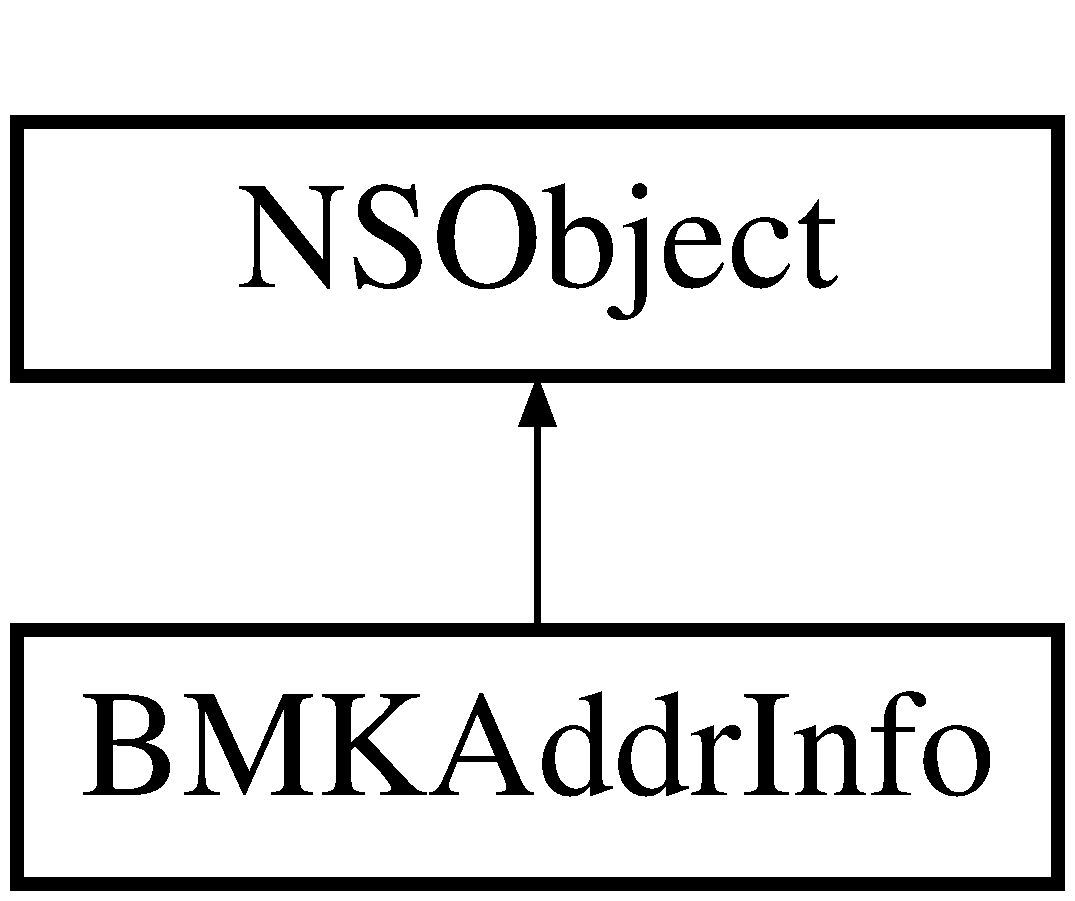
\includegraphics[height=2.000000cm]{interface_b_m_k_addr_info}
\end{center}
\end{figure}
\subsection*{保护成员变量}
\begin{DoxyCompactItemize}
\item 
\hypertarget{interface_b_m_k_addr_info_a82f04809725fe1e8306ef7ab75785454}{N\-S\-String $\ast$ {\bfseries \-\_\-str\-Addr}}\label{interface_b_m_k_addr_info_a82f04809725fe1e8306ef7ab75785454}

\item 
\hypertarget{interface_b_m_k_addr_info_abc03f0262eee50b80180bd79c8800c7c}{C\-L\-Location\-Coordinate2\-D {\bfseries \-\_\-geo\-Pt}}\label{interface_b_m_k_addr_info_abc03f0262eee50b80180bd79c8800c7c}

\item 
\hypertarget{interface_b_m_k_addr_info_a5144c8f6a58780898f56fdc125730fc2}{N\-S\-Array $\ast$ {\bfseries \-\_\-poi\-List}}\label{interface_b_m_k_addr_info_a5144c8f6a58780898f56fdc125730fc2}

\end{DoxyCompactItemize}
\subsection*{Properties}
\begin{DoxyCompactItemize}
\item 
\hypertarget{interface_b_m_k_addr_info_a74172df67446d717c97ae2bde1845c35}{\hyperlink{interface_b_m_k_geocoder_address_component}{B\-M\-K\-Geocoder\-Address\-Component} $\ast$ {\bfseries \-\_\-address\-Component}}\label{interface_b_m_k_addr_info_a74172df67446d717c97ae2bde1845c35}

\item 
\hypertarget{interface_b_m_k_addr_info_a9807441809f9f878c3f31840f9f94874}{\hyperlink{interface_b_m_k_geocoder_address_component}{B\-M\-K\-Geocoder\-Address\-Component} $\ast$ \hyperlink{interface_b_m_k_addr_info_a9807441809f9f878c3f31840f9f94874}{address\-Component}}\label{interface_b_m_k_addr_info_a9807441809f9f878c3f31840f9f94874}

\begin{DoxyCompactList}\small\item\em 层次化地址信息 \end{DoxyCompactList}\item 
\hypertarget{interface_b_m_k_addr_info_a69292c1009e0ffe42cf4763da7d204ef}{N\-S\-String $\ast$ \hyperlink{interface_b_m_k_addr_info_a69292c1009e0ffe42cf4763da7d204ef}{str\-Addr}}\label{interface_b_m_k_addr_info_a69292c1009e0ffe42cf4763da7d204ef}

\begin{DoxyCompactList}\small\item\em 地址名称 \end{DoxyCompactList}\item 
\hypertarget{interface_b_m_k_addr_info_a5722dacf97cdf54a4f56a2ab109156e4}{C\-L\-Location\-Coordinate2\-D \hyperlink{interface_b_m_k_addr_info_a5722dacf97cdf54a4f56a2ab109156e4}{geo\-Pt}}\label{interface_b_m_k_addr_info_a5722dacf97cdf54a4f56a2ab109156e4}

\begin{DoxyCompactList}\small\item\em 地址坐标 \end{DoxyCompactList}\item 
\hypertarget{interface_b_m_k_addr_info_a9a7bbe0c0071e04354e295d006486251}{N\-S\-Array $\ast$ \hyperlink{interface_b_m_k_addr_info_a9a7bbe0c0071e04354e295d006486251}{poi\-List}}\label{interface_b_m_k_addr_info_a9a7bbe0c0071e04354e295d006486251}

\begin{DoxyCompactList}\small\item\em 地址周边\-P\-O\-I信息,成员类型为\-B\-M\-K\-Poi\-Info \end{DoxyCompactList}\end{DoxyCompactItemize}


\subsection{详细描述}
地址信息类,用于地理编码和反地理编码 

The documentation for this class was generated from the following file\-:\begin{DoxyCompactItemize}
\item 
B\-M\-K\-Geocode\-Type.\-h\end{DoxyCompactItemize}

\hypertarget{protocol_b_m_k_annotation-p}{\section{$<$B\-M\-K\-Annotation$>$ 协议参考}
\label{protocol_b_m_k_annotation-p}\index{$<$\-B\-M\-K\-Annotation$>$@{$<$\-B\-M\-K\-Annotation$>$}}
}


该类为标注点的protocol,提供了标注类的基本信息函数  




{\ttfamily \#import $<$B\-M\-K\-Annotation.\-h$>$}

继承关系图 $<$B\-M\-K\-Annotation$>$\-:\begin{figure}[H]
\begin{center}
\leavevmode
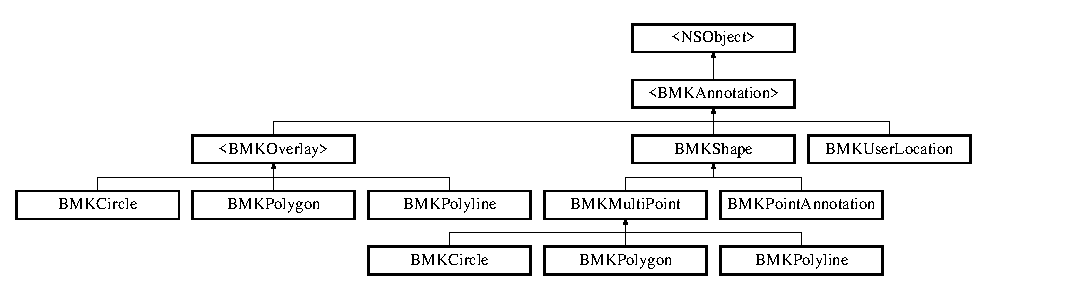
\includegraphics[height=3.456790cm]{protocol_b_m_k_annotation-p}
\end{center}
\end{figure}
\subsection*{实例方法}
\begin{DoxyCompactItemize}
\item 
(N\-S\-String $\ast$) -\/ \hyperlink{protocol_b_m_k_annotation-p_a249e1b880f8ded8541a0fe59ef4abb12}{title}
\item 
(N\-S\-String $\ast$) -\/ \hyperlink{protocol_b_m_k_annotation-p_a62aea71f4631251330e8a6fc3d3bdf11}{subtitle}
\item 
(void) -\/ \hyperlink{protocol_b_m_k_annotation-p_a86db1788af78d273e1e155d3aa3d978f}{set\-Coordinate\-:}
\end{DoxyCompactItemize}
\subsection*{Properties}
\begin{DoxyCompactItemize}
\item 
\hypertarget{protocol_b_m_k_annotation-p_ab7ed7fd80fc518acf82cf0048490f9be}{C\-L\-Location\-Coordinate2\-D \hyperlink{protocol_b_m_k_annotation-p_ab7ed7fd80fc518acf82cf0048490f9be}{coordinate}}\label{protocol_b_m_k_annotation-p_ab7ed7fd80fc518acf82cf0048490f9be}

\begin{DoxyCompactList}\small\item\em 标注view中心坐标. \end{DoxyCompactList}\end{DoxyCompactItemize}


\subsection{详细描述}
该类为标注点的protocol,提供了标注类的基本信息函数 

\subsection{方法文档}
\hypertarget{protocol_b_m_k_annotation-p_a86db1788af78d273e1e155d3aa3d978f}{\index{B\-M\-K\-Annotation-\/p@{B\-M\-K\-Annotation-\/p}!set\-Coordinate\-:@{set\-Coordinate\-:}}
\index{set\-Coordinate\-:@{set\-Coordinate\-:}!BMKAnnotation-p@{B\-M\-K\-Annotation-\/p}}
\subsubsection[{set\-Coordinate\-:}]{\setlength{\rightskip}{0pt plus 5cm}-\/ (void) set\-Coordinate\-: 
\begin{DoxyParamCaption}
\item[{(C\-L\-Location\-Coordinate2\-D)}]{new\-Coordinate}
\end{DoxyParamCaption}
\hspace{0.3cm}{\ttfamily [optional]}}}\label{protocol_b_m_k_annotation-p_a86db1788af78d273e1e155d3aa3d978f}
设置标注的坐标,在拖拽时会被调用. 
\begin{DoxyParams}{参数}
{\em new\-Coordinate} & 新的坐标值 \\
\hline
\end{DoxyParams}
\hypertarget{protocol_b_m_k_annotation-p_a62aea71f4631251330e8a6fc3d3bdf11}{\index{B\-M\-K\-Annotation-\/p@{B\-M\-K\-Annotation-\/p}!subtitle@{subtitle}}
\index{subtitle@{subtitle}!BMKAnnotation-p@{B\-M\-K\-Annotation-\/p}}
\subsubsection[{subtitle}]{\setlength{\rightskip}{0pt plus 5cm}-\/ (N\-S\-String $\ast$) subtitle 
\begin{DoxyParamCaption}
{}
\end{DoxyParamCaption}
\hspace{0.3cm}{\ttfamily [optional]}}}\label{protocol_b_m_k_annotation-p_a62aea71f4631251330e8a6fc3d3bdf11}
获取annotation副标题 \begin{DoxyReturn}{返回}
返回annotation的副标题信息 
\end{DoxyReturn}
\hypertarget{protocol_b_m_k_annotation-p_a249e1b880f8ded8541a0fe59ef4abb12}{\index{B\-M\-K\-Annotation-\/p@{B\-M\-K\-Annotation-\/p}!title@{title}}
\index{title@{title}!BMKAnnotation-p@{B\-M\-K\-Annotation-\/p}}
\subsubsection[{title}]{\setlength{\rightskip}{0pt plus 5cm}-\/ (N\-S\-String $\ast$) title 
\begin{DoxyParamCaption}
{}
\end{DoxyParamCaption}
\hspace{0.3cm}{\ttfamily [optional]}}}\label{protocol_b_m_k_annotation-p_a249e1b880f8ded8541a0fe59ef4abb12}
获取annotation标题 \begin{DoxyReturn}{返回}
返回annotation的标题信息 
\end{DoxyReturn}


The documentation for this protocol was generated from the following file\-:\begin{DoxyCompactItemize}
\item 
B\-M\-K\-Annotation.\-h\end{DoxyCompactItemize}

\hypertarget{interface_b_m_k_annotation_view}{\section{B\-M\-K\-Annotation\-View 类参考}
\label{interface_b_m_k_annotation_view}\index{B\-M\-K\-Annotation\-View@{B\-M\-K\-Annotation\-View}}
}


标注view  




{\ttfamily \#import $<$B\-M\-K\-Annotation\-View.\-h$>$}

继承关系图 B\-M\-K\-Annotation\-View\-:\begin{figure}[H]
\begin{center}
\leavevmode
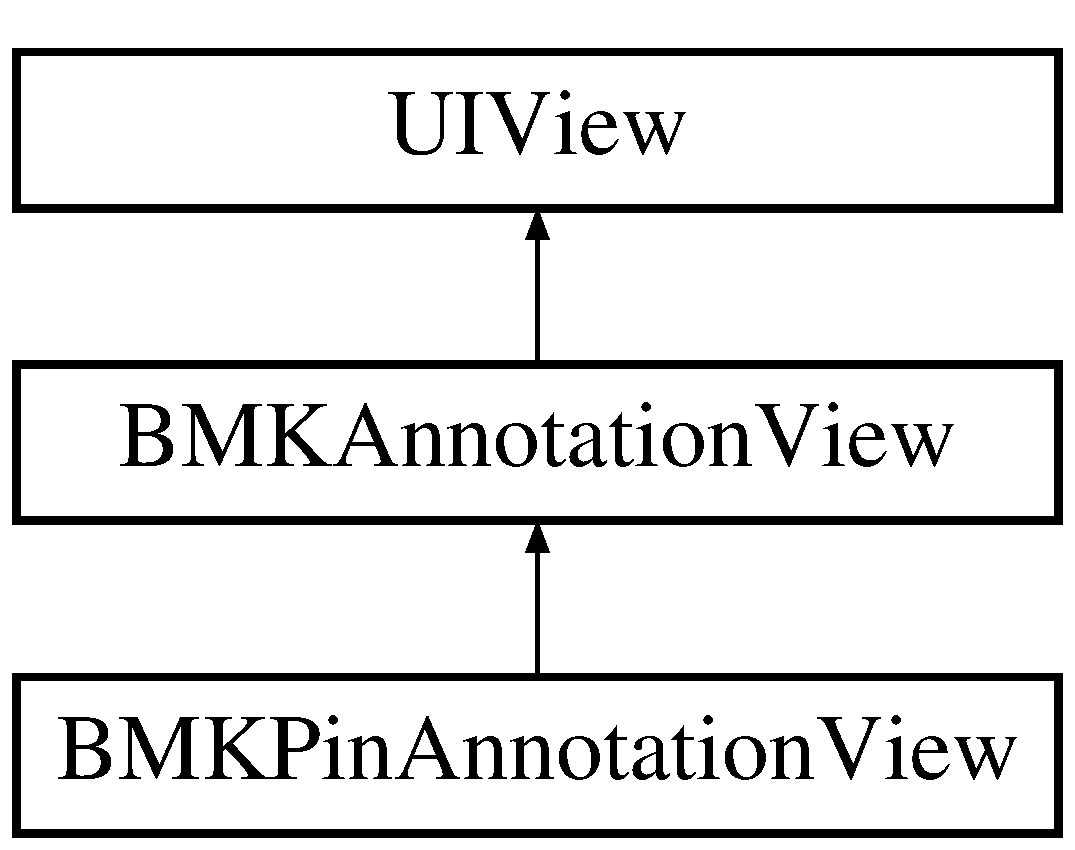
\includegraphics[height=3.000000cm]{interface_b_m_k_annotation_view}
\end{center}
\end{figure}
\subsection*{实例方法}
\begin{DoxyCompactItemize}
\item 
(id) -\/ \hyperlink{interface_b_m_k_annotation_view_ae2b46541ec52b7d8ee0857a9ec369f5f}{init\-With\-Annotation\-:reuse\-Identifier\-:}
\item 
(void) -\/ \hyperlink{interface_b_m_k_annotation_view_ae74849e624ac0cfaa7695b7cc97ddf23}{prepare\-For\-Reuse}
\item 
(void) -\/ \hyperlink{interface_b_m_k_annotation_view_abc0e70812fb7b3bccdbb574ddb578c21}{set\-Selected\-:animated\-:}
\item 
\hypertarget{interface_b_m_k_annotation_view_a54d15e7cc4e89d89d2233ec7fc408ad9}{(B\-O\-O\-L draggable) -\/ \hyperlink{interface_b_m_k_annotation_view_a54d15e7cc4e89d89d2233ec7fc408ad9}{\-\_\-\-\_\-\-O\-S\-X\-\_\-\-A\-V\-A\-I\-L\-A\-B\-L\-E\-\_\-\-S\-T\-A\-R\-T\-I\-N\-G}}\label{interface_b_m_k_annotation_view_a54d15e7cc4e89d89d2233ec7fc408ad9}

\begin{DoxyCompactList}\small\item\em 当设为\-Y\-E\-S并实现了set\-Coordinate\-:方法时,支持将view在地图上拖动, ios 3.\-2以后支持 \end{DoxyCompactList}\item 
\hypertarget{interface_b_m_k_annotation_view_a623e818d48c983176a6553104b21a34c}{(B\-M\-K\-Annotation\-View\-Drag\-State \\*
drag\-State) -\/ \hyperlink{interface_b_m_k_annotation_view_a623e818d48c983176a6553104b21a34c}{\-\_\-\-\_\-\-O\-S\-X\-\_\-\-A\-V\-A\-I\-L\-A\-B\-L\-E\-\_\-\-S\-T\-A\-R\-T\-I\-N\-G}}\label{interface_b_m_k_annotation_view_a623e818d48c983176a6553104b21a34c}

\begin{DoxyCompactList}\small\item\em 当前view的拖动状态, ios 3.\-2以后支持 \end{DoxyCompactList}\end{DoxyCompactItemize}
\subsection*{Properties}
\begin{DoxyCompactItemize}
\item 
\hypertarget{interface_b_m_k_annotation_view_aba3efdbef49c0301af03ce0d47348358}{N\-S\-String $\ast$ \hyperlink{interface_b_m_k_annotation_view_aba3efdbef49c0301af03ce0d47348358}{reuse\-Identifier}}\label{interface_b_m_k_annotation_view_aba3efdbef49c0301af03ce0d47348358}

\begin{DoxyCompactList}\small\item\em 复用标志 \end{DoxyCompactList}\item 
\hypertarget{interface_b_m_k_annotation_view_a45b607eff441e212a1dd7c6d5846f4e3}{U\-I\-View $\ast$ {\bfseries paopao\-View}}\label{interface_b_m_k_annotation_view_a45b607eff441e212a1dd7c6d5846f4e3}

\item 
\hypertarget{interface_b_m_k_annotation_view_a466f040671f2235667a4034aba879bb5}{id$<$ \hyperlink{protocol_b_m_k_annotation-p}{B\-M\-K\-Annotation} $>$ \hyperlink{interface_b_m_k_annotation_view_a466f040671f2235667a4034aba879bb5}{annotation}}\label{interface_b_m_k_annotation_view_a466f040671f2235667a4034aba879bb5}

\begin{DoxyCompactList}\small\item\em 关联的annotation \end{DoxyCompactList}\item 
\hypertarget{interface_b_m_k_annotation_view_a3186f78dcb098002e39fd226cbc1c9b6}{U\-I\-Image $\ast$ \hyperlink{interface_b_m_k_annotation_view_a3186f78dcb098002e39fd226cbc1c9b6}{image}}\label{interface_b_m_k_annotation_view_a3186f78dcb098002e39fd226cbc1c9b6}

\begin{DoxyCompactList}\small\item\em annotation view显示的图像 \end{DoxyCompactList}\item 
\hypertarget{interface_b_m_k_annotation_view_a12a4f32e8adc7732c80d772eb403cd61}{C\-G\-Point \hyperlink{interface_b_m_k_annotation_view_a12a4f32e8adc7732c80d772eb403cd61}{center\-Offset}}\label{interface_b_m_k_annotation_view_a12a4f32e8adc7732c80d772eb403cd61}

\begin{DoxyCompactList}\small\item\em 默认情况下, annotation view的中心位于annotation的坐标位置,可以设置center\-Offset改变view的位置,正的偏移使view朝右下方移动,负的朝左上方,单位是像素 \end{DoxyCompactList}\item 
\hypertarget{interface_b_m_k_annotation_view_aacdcb492cbbc469803ba50def87f44e5}{C\-G\-Point \hyperlink{interface_b_m_k_annotation_view_aacdcb492cbbc469803ba50def87f44e5}{callout\-Offset}}\label{interface_b_m_k_annotation_view_aacdcb492cbbc469803ba50def87f44e5}

\begin{DoxyCompactList}\small\item\em 默认情况下, 弹出的气泡位于view正中上方,可以设置callout\-Offset改变view的位置,正的偏移使view朝右下方移动,负的朝左上方,单位是像素 \end{DoxyCompactList}\item 
\hypertarget{interface_b_m_k_annotation_view_a18cef771d9b9feeb74a4bc4dd7fba526}{B\-O\-O\-L \hyperlink{interface_b_m_k_annotation_view_a18cef771d9b9feeb74a4bc4dd7fba526}{enabled3\-D}}\label{interface_b_m_k_annotation_view_a18cef771d9b9feeb74a4bc4dd7fba526}

\begin{DoxyCompactList}\small\item\em 默认情况下,标注没有3\-D效果,可以设置enabled3\-D改变使用3\-D效果,使得标注在地图旋转和俯视时跟随旋转、俯视 \end{DoxyCompactList}\item 
\hypertarget{interface_b_m_k_annotation_view_ad768885a75146458b4efd168885478fe}{B\-O\-O\-L \hyperlink{interface_b_m_k_annotation_view_ad768885a75146458b4efd168885478fe}{enabled}}\label{interface_b_m_k_annotation_view_ad768885a75146458b4efd168885478fe}

\begin{DoxyCompactList}\small\item\em 默认为\-Y\-E\-S,当为\-N\-O时view忽略触摸事件 \end{DoxyCompactList}\item 
\hypertarget{interface_b_m_k_annotation_view_a09799664ef861651bd7996f0fbab6483}{B\-O\-O\-L \hyperlink{interface_b_m_k_annotation_view_a09799664ef861651bd7996f0fbab6483}{selected}}\label{interface_b_m_k_annotation_view_a09799664ef861651bd7996f0fbab6483}

\begin{DoxyCompactList}\small\item\em 默认为\-N\-O,当view被点中时被设为\-Y\-E\-S,用户不要直接设置这个属性. \end{DoxyCompactList}\item 
\hypertarget{interface_b_m_k_annotation_view_adef94e946f5b152c59be1cdb5eccfb74}{B\-O\-O\-L \hyperlink{interface_b_m_k_annotation_view_adef94e946f5b152c59be1cdb5eccfb74}{can\-Show\-Callout}}\label{interface_b_m_k_annotation_view_adef94e946f5b152c59be1cdb5eccfb74}

\begin{DoxyCompactList}\small\item\em 当为\-Y\-E\-S时,view被选中时会弹出气泡,annotation必须实现了title这个方法 \end{DoxyCompactList}\item 
\hypertarget{interface_b_m_k_annotation_view_ae182c0fb7dc1898c4941a123def7f926}{U\-I\-View $\ast$ \hyperlink{interface_b_m_k_annotation_view_ae182c0fb7dc1898c4941a123def7f926}{left\-Callout\-Accessory\-View}}\label{interface_b_m_k_annotation_view_ae182c0fb7dc1898c4941a123def7f926}

\begin{DoxyCompactList}\small\item\em 显示在气泡左侧的view \end{DoxyCompactList}\item 
\hypertarget{interface_b_m_k_annotation_view_a65793288845c27e23233373b3e6b6216}{U\-I\-View $\ast$ \hyperlink{interface_b_m_k_annotation_view_a65793288845c27e23233373b3e6b6216}{right\-Callout\-Accessory\-View}}\label{interface_b_m_k_annotation_view_a65793288845c27e23233373b3e6b6216}

\begin{DoxyCompactList}\small\item\em 显示在气泡右侧的view \end{DoxyCompactList}\end{DoxyCompactItemize}


\subsection{详细描述}
标注view 

\subsection{方法文档}
\hypertarget{interface_b_m_k_annotation_view_ae2b46541ec52b7d8ee0857a9ec369f5f}{\index{B\-M\-K\-Annotation\-View@{B\-M\-K\-Annotation\-View}!init\-With\-Annotation\-:reuse\-Identifier\-:@{init\-With\-Annotation\-:reuse\-Identifier\-:}}
\index{init\-With\-Annotation\-:reuse\-Identifier\-:@{init\-With\-Annotation\-:reuse\-Identifier\-:}!BMKAnnotationView@{B\-M\-K\-Annotation\-View}}
\subsubsection[{init\-With\-Annotation\-:reuse\-Identifier\-:}]{\setlength{\rightskip}{0pt plus 5cm}-\/ (id) init\-With\-Annotation\-: 
\begin{DoxyParamCaption}
\item[{(id$<$ {\bf B\-M\-K\-Annotation} $>$)}]{annotation}
\item[{reuseIdentifier:(N\-S\-String $\ast$)}]{reuse\-Identifier}
\end{DoxyParamCaption}
}}\label{interface_b_m_k_annotation_view_ae2b46541ec52b7d8ee0857a9ec369f5f}
初始化并返回一个annotation view 
\begin{DoxyParams}{参数}
{\em annotation} & 关联的annotation对象 \\
\hline
{\em reuse\-Identifier} & 如果要重用view,传入一个字符串,否则设为nil,建议重用view \\
\hline
\end{DoxyParams}
\begin{DoxyReturn}{返回}
初始化成功则返回annotation view,否则返回nil 
\end{DoxyReturn}
\hypertarget{interface_b_m_k_annotation_view_ae74849e624ac0cfaa7695b7cc97ddf23}{\index{B\-M\-K\-Annotation\-View@{B\-M\-K\-Annotation\-View}!prepare\-For\-Reuse@{prepare\-For\-Reuse}}
\index{prepare\-For\-Reuse@{prepare\-For\-Reuse}!BMKAnnotationView@{B\-M\-K\-Annotation\-View}}
\subsubsection[{prepare\-For\-Reuse}]{\setlength{\rightskip}{0pt plus 5cm}-\/ (void) prepare\-For\-Reuse 
\begin{DoxyParamCaption}
{}
\end{DoxyParamCaption}
}}\label{interface_b_m_k_annotation_view_ae74849e624ac0cfaa7695b7cc97ddf23}
当view从reuse队列里取出时被调用 默认不做任何事 \hypertarget{interface_b_m_k_annotation_view_abc0e70812fb7b3bccdbb574ddb578c21}{\index{B\-M\-K\-Annotation\-View@{B\-M\-K\-Annotation\-View}!set\-Selected\-:animated\-:@{set\-Selected\-:animated\-:}}
\index{set\-Selected\-:animated\-:@{set\-Selected\-:animated\-:}!BMKAnnotationView@{B\-M\-K\-Annotation\-View}}
\subsubsection[{set\-Selected\-:animated\-:}]{\setlength{\rightskip}{0pt plus 5cm}-\/ (void) set\-Selected\-: 
\begin{DoxyParamCaption}
\item[{(B\-O\-O\-L)}]{selected}
\item[{animated:(B\-O\-O\-L)}]{animated}
\end{DoxyParamCaption}
}}\label{interface_b_m_k_annotation_view_abc0e70812fb7b3bccdbb574ddb578c21}
设定view的选中状态 该方法被\-B\-M\-K\-Map\-View调用 
\begin{DoxyParams}{参数}
{\em selected} & 如果view需要显示为选中状态,该值为\-Y\-E\-S \\
\hline
{\em animated} & 如果需要动画效果,该值为\-Y\-E\-S,暂不支持 \\
\hline
\end{DoxyParams}


The documentation for this class was generated from the following file\-:\begin{DoxyCompactItemize}
\item 
B\-M\-K\-Annotation\-View.\-h\end{DoxyCompactItemize}

\hypertarget{interface_b_m_k_bus_line_result}{\section{B\-M\-K\-Bus\-Line\-Result 类参考}
\label{interface_b_m_k_bus_line_result}\index{B\-M\-K\-Bus\-Line\-Result@{B\-M\-K\-Bus\-Line\-Result}}
}


公交详情结果类.  




{\ttfamily \#import $<$B\-M\-K\-Route\-Search\-Type.\-h$>$}

继承关系图 B\-M\-K\-Bus\-Line\-Result\-:\begin{figure}[H]
\begin{center}
\leavevmode
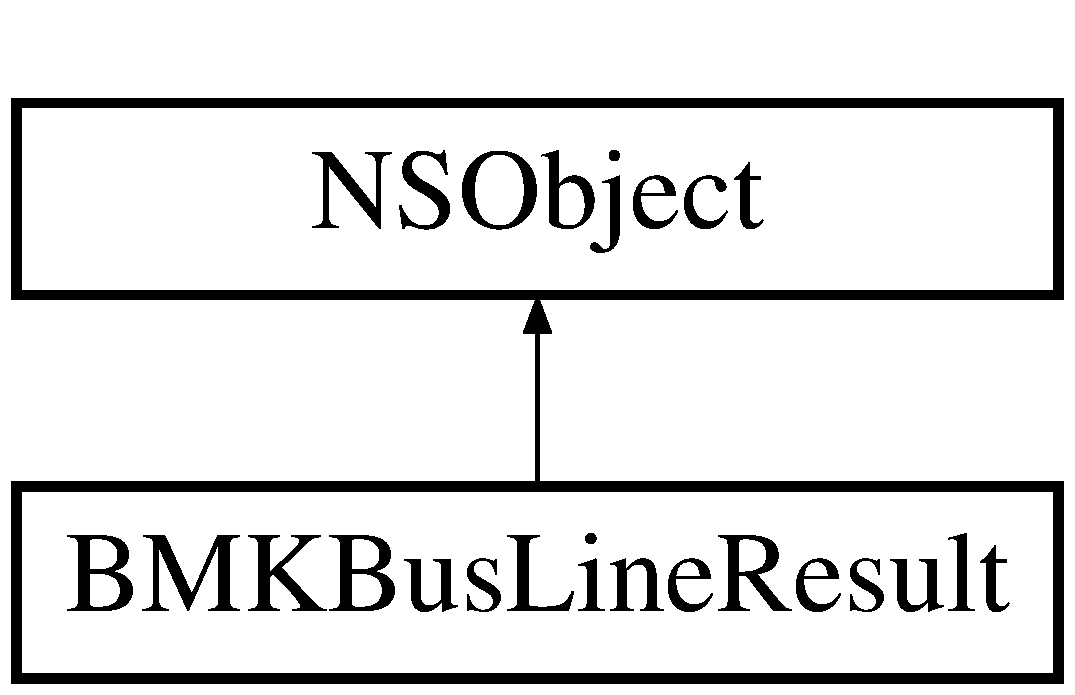
\includegraphics[height=2.000000cm]{interface_b_m_k_bus_line_result}
\end{center}
\end{figure}
\subsection*{保护成员变量}
\begin{DoxyCompactItemize}
\item 
\hypertarget{interface_b_m_k_bus_line_result_abc69157a4b302e25f834d22718f6d0f7}{N\-S\-String $\ast$ {\bfseries \-\_\-m\-Bus\-Name}}\label{interface_b_m_k_bus_line_result_abc69157a4b302e25f834d22718f6d0f7}

\item 
\hypertarget{interface_b_m_k_bus_line_result_a00071f4e6289bf9506f5d9928dfbdaea}{int {\bfseries \-\_\-m\-Is\-Mon\-Ticket}}\label{interface_b_m_k_bus_line_result_a00071f4e6289bf9506f5d9928dfbdaea}

\item 
\hypertarget{interface_b_m_k_bus_line_result_aacca8d8685fbbd9c69b2129104197f14}{N\-S\-String $\ast$ {\bfseries \-\_\-m\-Start\-Time}}\label{interface_b_m_k_bus_line_result_aacca8d8685fbbd9c69b2129104197f14}

\item 
\hypertarget{interface_b_m_k_bus_line_result_add4d8cfb78c543c01f4ec126a81950c7}{N\-S\-String $\ast$ {\bfseries \-\_\-m\-End\-Time}}\label{interface_b_m_k_bus_line_result_add4d8cfb78c543c01f4ec126a81950c7}

\item 
\hypertarget{interface_b_m_k_bus_line_result_aaec01789f4b09de0017b54651c4be14d}{\hyperlink{interface_b_m_k_route}{B\-M\-K\-Route} $\ast$ {\bfseries \-\_\-m\-Bus\-Route}}\label{interface_b_m_k_bus_line_result_aaec01789f4b09de0017b54651c4be14d}

\end{DoxyCompactItemize}
\subsection*{Properties}
\begin{DoxyCompactItemize}
\item 
\hypertarget{interface_b_m_k_bus_line_result_ae220e8f61d63bc810e2fcec3cbba716d}{N\-S\-String $\ast$ {\bfseries \-\_\-m\-Company}}\label{interface_b_m_k_bus_line_result_ae220e8f61d63bc810e2fcec3cbba716d}

\item 
\hypertarget{interface_b_m_k_bus_line_result_ac69981cd28c6d7c5b20d47b3192c5d68}{N\-S\-String $\ast$ {\bfseries m\-Company}}\label{interface_b_m_k_bus_line_result_ac69981cd28c6d7c5b20d47b3192c5d68}

\item 
\hypertarget{interface_b_m_k_bus_line_result_ae33b464d9523ee4f6a02d281d0ba6e13}{N\-S\-String $\ast$ {\bfseries m\-Bus\-Name}}\label{interface_b_m_k_bus_line_result_ae33b464d9523ee4f6a02d281d0ba6e13}

\item 
\hypertarget{interface_b_m_k_bus_line_result_a058b38950a97101d275bcf8a1a2663c7}{int {\bfseries m\-Is\-Mon\-Ticket}}\label{interface_b_m_k_bus_line_result_a058b38950a97101d275bcf8a1a2663c7}

\item 
\hypertarget{interface_b_m_k_bus_line_result_a5627fd4b44b2bb27f899a42d2bc6ba65}{N\-S\-String $\ast$ {\bfseries m\-Start\-Time}}\label{interface_b_m_k_bus_line_result_a5627fd4b44b2bb27f899a42d2bc6ba65}

\item 
\hypertarget{interface_b_m_k_bus_line_result_aa2e675ce53aaa766fabdb0052dc7ba10}{N\-S\-String $\ast$ {\bfseries m\-End\-Time}}\label{interface_b_m_k_bus_line_result_aa2e675ce53aaa766fabdb0052dc7ba10}

\item 
\hypertarget{interface_b_m_k_bus_line_result_ae3befda89bc1866b9ffdca02a6f5a80a}{\hyperlink{interface_b_m_k_route}{B\-M\-K\-Route} $\ast$ {\bfseries m\-Bus\-Route}}\label{interface_b_m_k_bus_line_result_ae3befda89bc1866b9ffdca02a6f5a80a}

\end{DoxyCompactItemize}


\subsection{详细描述}
公交详情结果类. 

The documentation for this class was generated from the following file\-:\begin{DoxyCompactItemize}
\item 
B\-M\-K\-Route\-Search\-Type.\-h\end{DoxyCompactItemize}

\hypertarget{interface_b_m_k_circle}{\section{B\-M\-K\-Circle 类参考}
\label{interface_b_m_k_circle}\index{B\-M\-K\-Circle@{B\-M\-K\-Circle}}
}


该类用于定义一个圆  




{\ttfamily \#import $<$B\-M\-K\-Circle.\-h$>$}

继承关系图 B\-M\-K\-Circle\-:\begin{figure}[H]
\begin{center}
\leavevmode
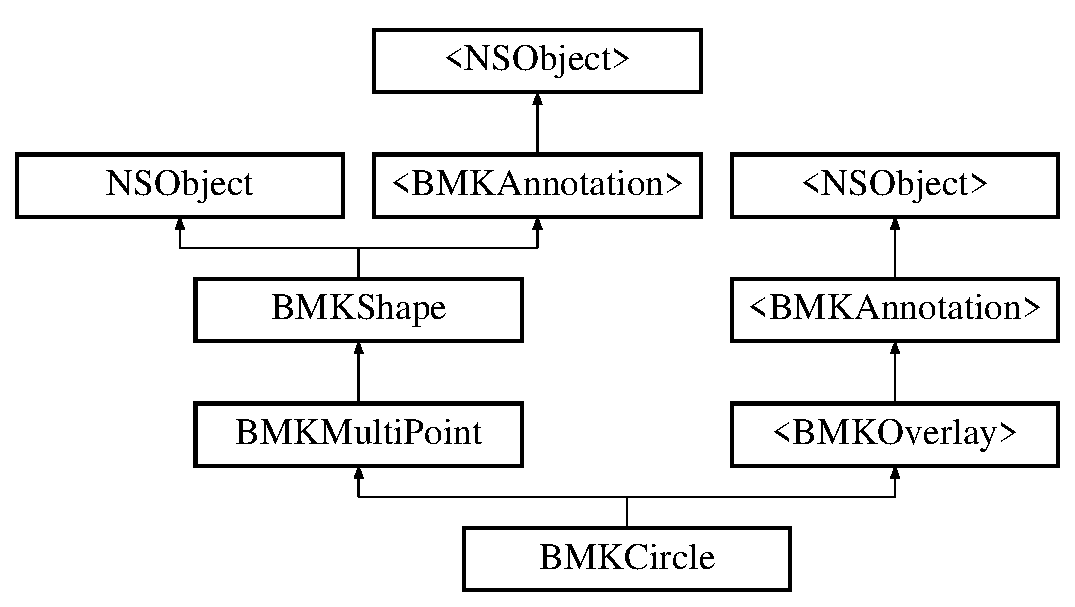
\includegraphics[height=5.000000cm]{interface_b_m_k_circle}
\end{center}
\end{figure}
\subsection*{类方法}
\begin{DoxyCompactItemize}
\item 
(\hyperlink{interface_b_m_k_circle}{B\-M\-K\-Circle} $\ast$) + \hyperlink{interface_b_m_k_circle_a82a7234e92fda719b74d6055ee30d360}{circle\-With\-Center\-Coordinate\-:radius\-:}
\item 
(\hyperlink{interface_b_m_k_circle}{B\-M\-K\-Circle} $\ast$) + \hyperlink{interface_b_m_k_circle_af4109f36f784b80a758a0b48c636e4a7}{circle\-With\-Map\-Rect\-:}
\end{DoxyCompactItemize}
\subsection*{保护成员变量}
\begin{DoxyCompactItemize}
\item 
\hypertarget{interface_b_m_k_circle_a66cd02759b46e5f8eb0370c40642cac1}{package C\-L\-Location\-Coordinate2\-D {\bfseries \-\_\-coordinate}}\label{interface_b_m_k_circle_a66cd02759b46e5f8eb0370c40642cac1}

\item 
\hypertarget{interface_b_m_k_circle_a84860dbbaa96509cfa4c7590908aabe8}{C\-L\-Location\-Distance {\bfseries \-\_\-radius}}\label{interface_b_m_k_circle_a84860dbbaa96509cfa4c7590908aabe8}

\item 
\hypertarget{interface_b_m_k_circle_abfa42e25c856dd426fb74b9531e1061b}{\hyperlink{struct_b_m_k_map_rect}{B\-M\-K\-Map\-Rect} {\bfseries \-\_\-bounding\-Map\-Rect}}\label{interface_b_m_k_circle_abfa42e25c856dd426fb74b9531e1061b}

\end{DoxyCompactItemize}
\subsection*{Properties}
\begin{DoxyCompactItemize}
\item 
\hypertarget{interface_b_m_k_circle_a1c516c10dec1971c686e07f814f333f9}{C\-L\-Location\-Coordinate2\-D \hyperlink{interface_b_m_k_circle_a1c516c10dec1971c686e07f814f333f9}{coordinate}}\label{interface_b_m_k_circle_a1c516c10dec1971c686e07f814f333f9}

\begin{DoxyCompactList}\small\item\em 中心点坐标 \end{DoxyCompactList}\item 
\hypertarget{interface_b_m_k_circle_a42507e4c17b4a1c1309fcbe06e370bf5}{C\-L\-Location\-Distance \hyperlink{interface_b_m_k_circle_a42507e4c17b4a1c1309fcbe06e370bf5}{radius}}\label{interface_b_m_k_circle_a42507e4c17b4a1c1309fcbe06e370bf5}

\begin{DoxyCompactList}\small\item\em 半径,单位:米 \end{DoxyCompactList}\item 
\hypertarget{interface_b_m_k_circle_a462a1696e47b1523dd481b22d43bcf46}{\hyperlink{struct_b_m_k_map_rect}{B\-M\-K\-Map\-Rect} \hyperlink{interface_b_m_k_circle_a462a1696e47b1523dd481b22d43bcf46}{bounding\-Map\-Rect}}\label{interface_b_m_k_circle_a462a1696e47b1523dd481b22d43bcf46}

\begin{DoxyCompactList}\small\item\em 该圆的外接矩形 \end{DoxyCompactList}\end{DoxyCompactItemize}
\subsection*{附加继承成员}


\subsection{详细描述}
该类用于定义一个圆 

\subsection{方法文档}
\hypertarget{interface_b_m_k_circle_a82a7234e92fda719b74d6055ee30d360}{\index{B\-M\-K\-Circle@{B\-M\-K\-Circle}!circle\-With\-Center\-Coordinate\-:radius\-:@{circle\-With\-Center\-Coordinate\-:radius\-:}}
\index{circle\-With\-Center\-Coordinate\-:radius\-:@{circle\-With\-Center\-Coordinate\-:radius\-:}!BMKCircle@{B\-M\-K\-Circle}}
\subsubsection[{circle\-With\-Center\-Coordinate\-:radius\-:}]{\setlength{\rightskip}{0pt plus 5cm}+ ({\bf B\-M\-K\-Circle} $\ast$) circle\-With\-Center\-Coordinate\-: 
\begin{DoxyParamCaption}
\item[{(C\-L\-Location\-Coordinate2\-D)}]{coord}
\item[{radius:(C\-L\-Location\-Distance)}]{radius}
\end{DoxyParamCaption}
}}\label{interface_b_m_k_circle_a82a7234e92fda719b74d6055ee30d360}
根据中心点和半径生成圆 
\begin{DoxyParams}{参数}
{\em coord} & 中心点的经纬度坐标 \\
\hline
{\em radius} & 半径,单位:米 \\
\hline
\end{DoxyParams}
\begin{DoxyReturn}{返回}
新生成的圆 
\end{DoxyReturn}
\hypertarget{interface_b_m_k_circle_af4109f36f784b80a758a0b48c636e4a7}{\index{B\-M\-K\-Circle@{B\-M\-K\-Circle}!circle\-With\-Map\-Rect\-:@{circle\-With\-Map\-Rect\-:}}
\index{circle\-With\-Map\-Rect\-:@{circle\-With\-Map\-Rect\-:}!BMKCircle@{B\-M\-K\-Circle}}
\subsubsection[{circle\-With\-Map\-Rect\-:}]{\setlength{\rightskip}{0pt plus 5cm}+ ({\bf B\-M\-K\-Circle} $\ast$) circle\-With\-Map\-Rect\-: 
\begin{DoxyParamCaption}
\item[{({\bf B\-M\-K\-Map\-Rect})}]{map\-Rect}
\end{DoxyParamCaption}
}}\label{interface_b_m_k_circle_af4109f36f784b80a758a0b48c636e4a7}
根据指定的直角坐标矩形生成圆,半径由较长的那条边决定,radius = M\-A\-X(width, height)/2 
\begin{DoxyParams}{参数}
{\em map\-Rect} & 指定的直角坐标矩形 \\
\hline
\end{DoxyParams}
\begin{DoxyReturn}{返回}
新生成的圆 
\end{DoxyReturn}


The documentation for this class was generated from the following file\-:\begin{DoxyCompactItemize}
\item 
B\-M\-K\-Circle.\-h\end{DoxyCompactItemize}

\hypertarget{interface_b_m_k_circle_view}{\section{B\-M\-K\-Circle\-View 类参考}
\label{interface_b_m_k_circle_view}\index{B\-M\-K\-Circle\-View@{B\-M\-K\-Circle\-View}}
}


该类用于定义圆对应的\-View  




{\ttfamily \#import $<$B\-M\-K\-Circle\-View.\-h$>$}

继承关系图 B\-M\-K\-Circle\-View\-:\begin{figure}[H]
\begin{center}
\leavevmode
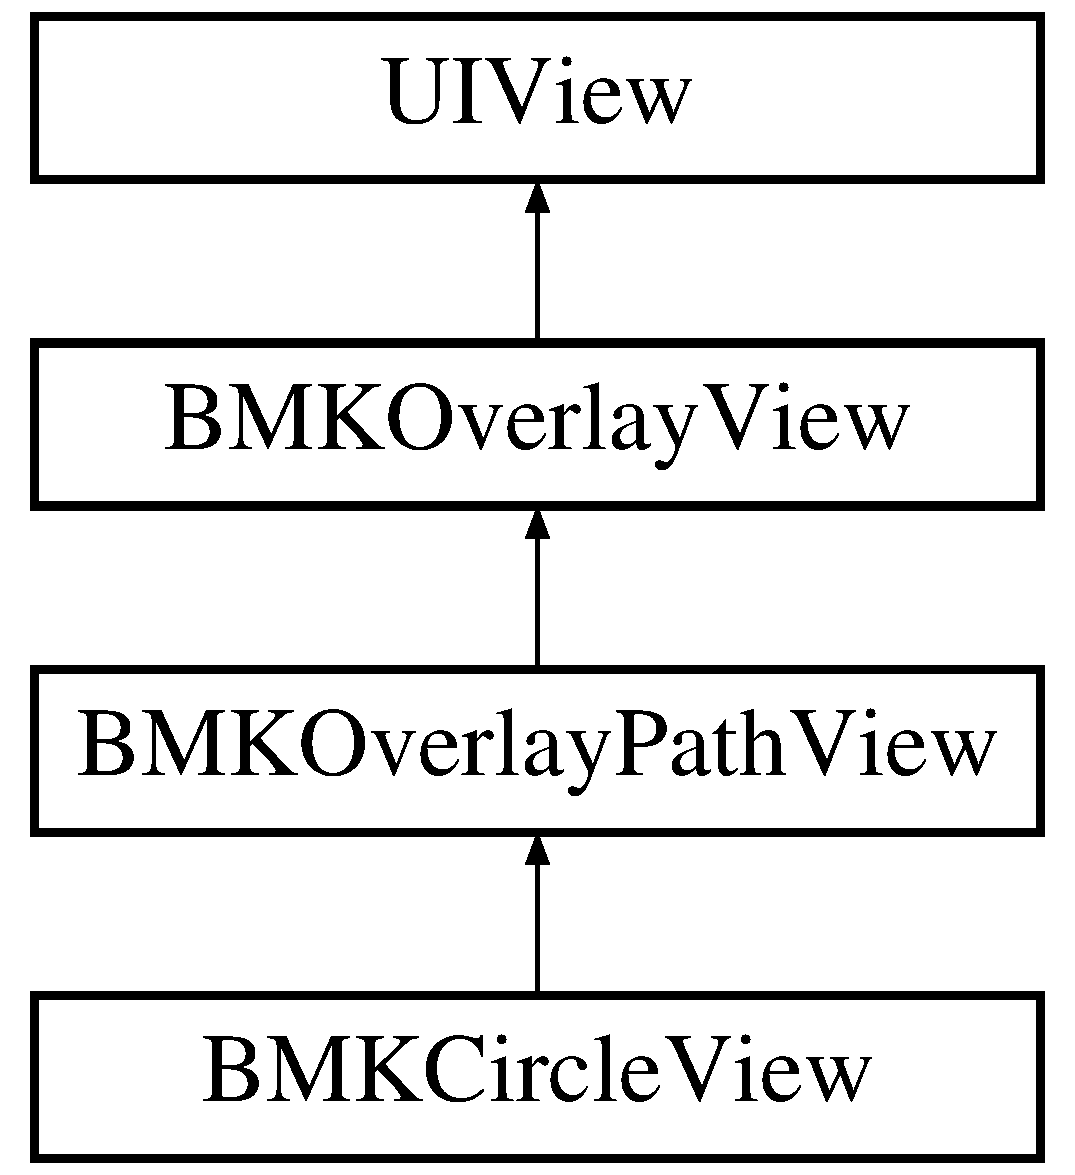
\includegraphics[height=4.000000cm]{interface_b_m_k_circle_view}
\end{center}
\end{figure}
\subsection*{实例方法}
\begin{DoxyCompactItemize}
\item 
(id) -\/ \hyperlink{interface_b_m_k_circle_view_a35f06526cf5423a39d434edc0517d34e}{init\-With\-Circle\-:}
\end{DoxyCompactItemize}
\subsection*{Properties}
\begin{DoxyCompactItemize}
\item 
\hypertarget{interface_b_m_k_circle_view_a07fe8c131d40bb225849dbc9bfb17e18}{\hyperlink{interface_b_m_k_circle}{B\-M\-K\-Circle} $\ast$ \hyperlink{interface_b_m_k_circle_view_a07fe8c131d40bb225849dbc9bfb17e18}{circle}}\label{interface_b_m_k_circle_view_a07fe8c131d40bb225849dbc9bfb17e18}

\begin{DoxyCompactList}\small\item\em 该\-View对应的圆 \end{DoxyCompactList}\end{DoxyCompactItemize}
\subsection*{附加继承成员}


\subsection{详细描述}
该类用于定义圆对应的\-View 

\subsection{方法文档}
\hypertarget{interface_b_m_k_circle_view_a35f06526cf5423a39d434edc0517d34e}{\index{B\-M\-K\-Circle\-View@{B\-M\-K\-Circle\-View}!init\-With\-Circle\-:@{init\-With\-Circle\-:}}
\index{init\-With\-Circle\-:@{init\-With\-Circle\-:}!BMKCircleView@{B\-M\-K\-Circle\-View}}
\subsubsection[{init\-With\-Circle\-:}]{\setlength{\rightskip}{0pt plus 5cm}-\/ (id) init\-With\-Circle\-: 
\begin{DoxyParamCaption}
\item[{({\bf B\-M\-K\-Circle} $\ast$)}]{circle}
\end{DoxyParamCaption}
}}\label{interface_b_m_k_circle_view_a35f06526cf5423a39d434edc0517d34e}
根据指定圆生成对应的\-View 
\begin{DoxyParams}{参数}
{\em circle} & 指定的圆 \\
\hline
\end{DoxyParams}
\begin{DoxyReturn}{返回}
生成的\-View 
\end{DoxyReturn}


The documentation for this class was generated from the following file\-:\begin{DoxyCompactItemize}
\item 
B\-M\-K\-Circle\-View.\-h\end{DoxyCompactItemize}

\hypertarget{interface_b_m_k_city_list_info}{\section{B\-M\-K\-City\-List\-Info 类参考}
\label{interface_b_m_k_city_list_info}\index{B\-M\-K\-City\-List\-Info@{B\-M\-K\-City\-List\-Info}}
}


城市列表信息类  




{\ttfamily \#import $<$B\-M\-K\-Poi\-Search\-Type.\-h$>$}

继承关系图 B\-M\-K\-City\-List\-Info\-:\begin{figure}[H]
\begin{center}
\leavevmode
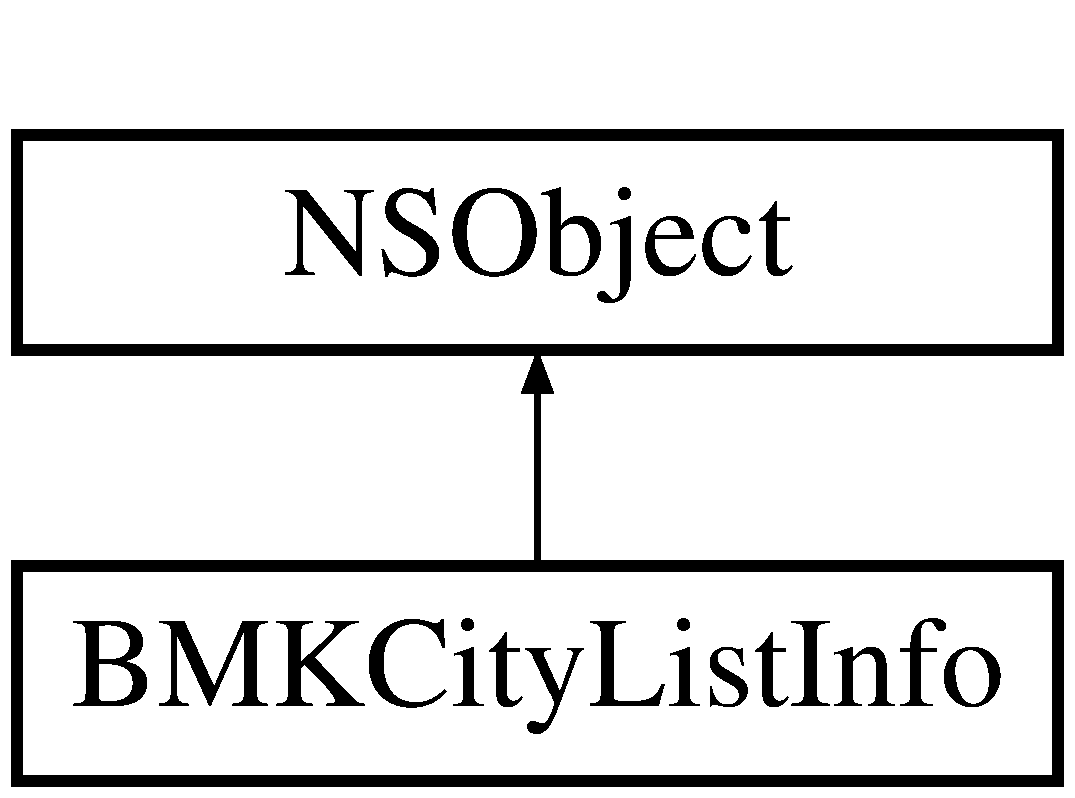
\includegraphics[height=2.000000cm]{interface_b_m_k_city_list_info}
\end{center}
\end{figure}
\subsection*{保护成员变量}
\begin{DoxyCompactItemize}
\item 
\hypertarget{interface_b_m_k_city_list_info_a868f1df35a24867c0957420506703225}{N\-S\-String $\ast$ {\bfseries \-\_\-city}}\label{interface_b_m_k_city_list_info_a868f1df35a24867c0957420506703225}

\item 
\hypertarget{interface_b_m_k_city_list_info_a0cc9abd0bfad17b52c924611f975db77}{int {\bfseries \-\_\-num}}\label{interface_b_m_k_city_list_info_a0cc9abd0bfad17b52c924611f975db77}

\end{DoxyCompactItemize}
\subsection*{Properties}
\begin{DoxyCompactItemize}
\item 
\hypertarget{interface_b_m_k_city_list_info_ad1b2093344ad0524a9bef93c823f8242}{N\-S\-String $\ast$ \hyperlink{interface_b_m_k_city_list_info_ad1b2093344ad0524a9bef93c823f8242}{city}}\label{interface_b_m_k_city_list_info_ad1b2093344ad0524a9bef93c823f8242}

\begin{DoxyCompactList}\small\item\em 城市名称 \end{DoxyCompactList}\item 
\hypertarget{interface_b_m_k_city_list_info_a63163c524339e1687d90541b3a24b54c}{int \hyperlink{interface_b_m_k_city_list_info_a63163c524339e1687d90541b3a24b54c}{num}}\label{interface_b_m_k_city_list_info_a63163c524339e1687d90541b3a24b54c}

\begin{DoxyCompactList}\small\item\em 该城市所含搜索结果数目 \end{DoxyCompactList}\end{DoxyCompactItemize}


\subsection{详细描述}
城市列表信息类 

The documentation for this class was generated from the following file\-:\begin{DoxyCompactItemize}
\item 
B\-M\-K\-Poi\-Search\-Type.\-h\end{DoxyCompactItemize}

\hypertarget{struct_b_m_k_coordinate_region}{\section{B\-M\-K\-Coordinate\-Region Struct Reference}
\label{struct_b_m_k_coordinate_region}\index{B\-M\-K\-Coordinate\-Region@{B\-M\-K\-Coordinate\-Region}}
}


表示一个经纬度区域  




{\ttfamily \#include $<$B\-M\-K\-Geometry.\-h$>$}

\subsection*{公有成员变量}
\begin{DoxyCompactItemize}
\item 
\hypertarget{struct_b_m_k_coordinate_region_a298c069df033a5690fdebc3c63f86903}{C\-L\-Location\-Coordinate2\-D \hyperlink{struct_b_m_k_coordinate_region_a298c069df033a5690fdebc3c63f86903}{center}}\label{struct_b_m_k_coordinate_region_a298c069df033a5690fdebc3c63f86903}

\begin{DoxyCompactList}\small\item\em 中心点经纬度坐标 \end{DoxyCompactList}\item 
\hypertarget{struct_b_m_k_coordinate_region_a75e65758cbbf7cb3ed6007d4ce301292}{\hyperlink{struct_b_m_k_coordinate_span}{B\-M\-K\-Coordinate\-Span} \hyperlink{struct_b_m_k_coordinate_region_a75e65758cbbf7cb3ed6007d4ce301292}{span}}\label{struct_b_m_k_coordinate_region_a75e65758cbbf7cb3ed6007d4ce301292}

\begin{DoxyCompactList}\small\item\em 经纬度范围 \end{DoxyCompactList}\end{DoxyCompactItemize}


\subsection{详细描述}
表示一个经纬度区域 

The documentation for this struct was generated from the following file\-:\begin{DoxyCompactItemize}
\item 
\hyperlink{_b_m_k_geometry_8h}{B\-M\-K\-Geometry.\-h}\end{DoxyCompactItemize}

\hypertarget{struct_b_m_k_coordinate_span}{\section{B\-M\-K\-Coordinate\-Span Struct Reference}
\label{struct_b_m_k_coordinate_span}\index{B\-M\-K\-Coordinate\-Span@{B\-M\-K\-Coordinate\-Span}}
}


表示一个经纬度范围  




{\ttfamily \#include $<$B\-M\-K\-Geometry.\-h$>$}

\subsection*{公有成员变量}
\begin{DoxyCompactItemize}
\item 
\hypertarget{struct_b_m_k_coordinate_span_a759543f626366ce4fe599b8896f352a2}{C\-L\-Location\-Degrees \hyperlink{struct_b_m_k_coordinate_span_a759543f626366ce4fe599b8896f352a2}{latitude\-Delta}}\label{struct_b_m_k_coordinate_span_a759543f626366ce4fe599b8896f352a2}

\begin{DoxyCompactList}\small\item\em 纬度范围 \end{DoxyCompactList}\item 
\hypertarget{struct_b_m_k_coordinate_span_ab3bc7d18bbd0fce7c806c51f0e0df447}{C\-L\-Location\-Degrees \hyperlink{struct_b_m_k_coordinate_span_ab3bc7d18bbd0fce7c806c51f0e0df447}{longitude\-Delta}}\label{struct_b_m_k_coordinate_span_ab3bc7d18bbd0fce7c806c51f0e0df447}

\begin{DoxyCompactList}\small\item\em 经度范围 \end{DoxyCompactList}\end{DoxyCompactItemize}


\subsection{详细描述}
表示一个经纬度范围 

The documentation for this struct was generated from the following file\-:\begin{DoxyCompactItemize}
\item 
\hyperlink{_b_m_k_geometry_8h}{B\-M\-K\-Geometry.\-h}\end{DoxyCompactItemize}

\hypertarget{protocol_b_m_k_general_delegate-p}{\section{$<$B\-M\-K\-General\-Delegate$>$ 协议参考}
\label{protocol_b_m_k_general_delegate-p}\index{$<$\-B\-M\-K\-General\-Delegate$>$@{$<$\-B\-M\-K\-General\-Delegate$>$}}
}


通知\-Delegate  




{\ttfamily \#import $<$B\-M\-K\-General\-Delegate.\-h$>$}

继承关系图 $<$B\-M\-K\-General\-Delegate$>$\-:\begin{figure}[H]
\begin{center}
\leavevmode
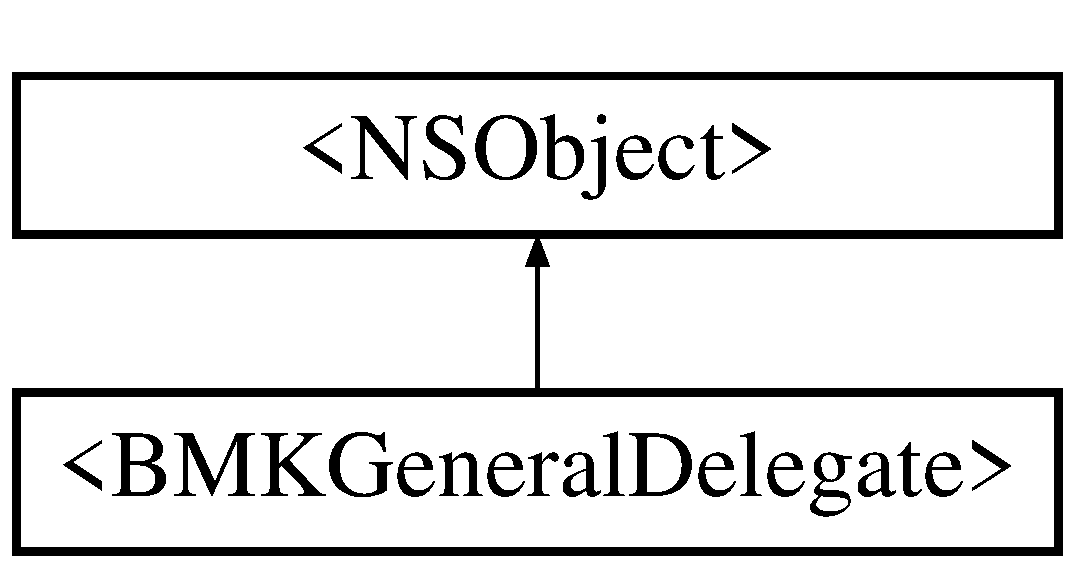
\includegraphics[height=2.000000cm]{protocol_b_m_k_general_delegate-p}
\end{center}
\end{figure}
\subsection*{实例方法}
\begin{DoxyCompactItemize}
\item 
(void) -\/ \hyperlink{protocol_b_m_k_general_delegate-p_ad30d0a4dc9bb54cda10cb892ed769491}{on\-Get\-Network\-State\-:}
\item 
(void) -\/ \hyperlink{protocol_b_m_k_general_delegate-p_ab0c34f007a8be34196fc81f2c7b3cddb}{on\-Get\-Permission\-State\-:}
\end{DoxyCompactItemize}


\subsection{详细描述}
通知\-Delegate 

\subsection{方法文档}
\hypertarget{protocol_b_m_k_general_delegate-p_ad30d0a4dc9bb54cda10cb892ed769491}{\index{B\-M\-K\-General\-Delegate-\/p@{B\-M\-K\-General\-Delegate-\/p}!on\-Get\-Network\-State\-:@{on\-Get\-Network\-State\-:}}
\index{on\-Get\-Network\-State\-:@{on\-Get\-Network\-State\-:}!BMKGeneralDelegate-p@{B\-M\-K\-General\-Delegate-\/p}}
\subsubsection[{on\-Get\-Network\-State\-:}]{\setlength{\rightskip}{0pt plus 5cm}-\/ (void) on\-Get\-Network\-State\-: 
\begin{DoxyParamCaption}
\item[{(int)}]{i\-Error}
\end{DoxyParamCaption}
\hspace{0.3cm}{\ttfamily [optional]}}}\label{protocol_b_m_k_general_delegate-p_ad30d0a4dc9bb54cda10cb892ed769491}
返回网络错误 
\begin{DoxyParams}{参数}
{\em i\-Error} & 错误号 \\
\hline
\end{DoxyParams}
\hypertarget{protocol_b_m_k_general_delegate-p_ab0c34f007a8be34196fc81f2c7b3cddb}{\index{B\-M\-K\-General\-Delegate-\/p@{B\-M\-K\-General\-Delegate-\/p}!on\-Get\-Permission\-State\-:@{on\-Get\-Permission\-State\-:}}
\index{on\-Get\-Permission\-State\-:@{on\-Get\-Permission\-State\-:}!BMKGeneralDelegate-p@{B\-M\-K\-General\-Delegate-\/p}}
\subsubsection[{on\-Get\-Permission\-State\-:}]{\setlength{\rightskip}{0pt plus 5cm}-\/ (void) on\-Get\-Permission\-State\-: 
\begin{DoxyParamCaption}
\item[{(int)}]{i\-Error}
\end{DoxyParamCaption}
\hspace{0.3cm}{\ttfamily [optional]}}}\label{protocol_b_m_k_general_delegate-p_ab0c34f007a8be34196fc81f2c7b3cddb}
返回授权验证错误 
\begin{DoxyParams}{参数}
{\em i\-Error} & 错误号 \-: B\-M\-K\-Error\-Permission\-Check\-Failure 验证失败 \\
\hline
\end{DoxyParams}


The documentation for this protocol was generated from the following file\-:\begin{DoxyCompactItemize}
\item 
B\-M\-K\-General\-Delegate.\-h\end{DoxyCompactItemize}

\hypertarget{interface_b_m_k_geocoder_address_component}{\section{B\-M\-K\-Geocoder\-Address\-Component 类参考}
\label{interface_b_m_k_geocoder_address_component}\index{B\-M\-K\-Geocoder\-Address\-Component@{B\-M\-K\-Geocoder\-Address\-Component}}
}


此类表示地址结果的层次化信息  




{\ttfamily \#import $<$B\-M\-K\-Geocode\-Type.\-h$>$}

继承关系图 B\-M\-K\-Geocoder\-Address\-Component\-:\begin{figure}[H]
\begin{center}
\leavevmode
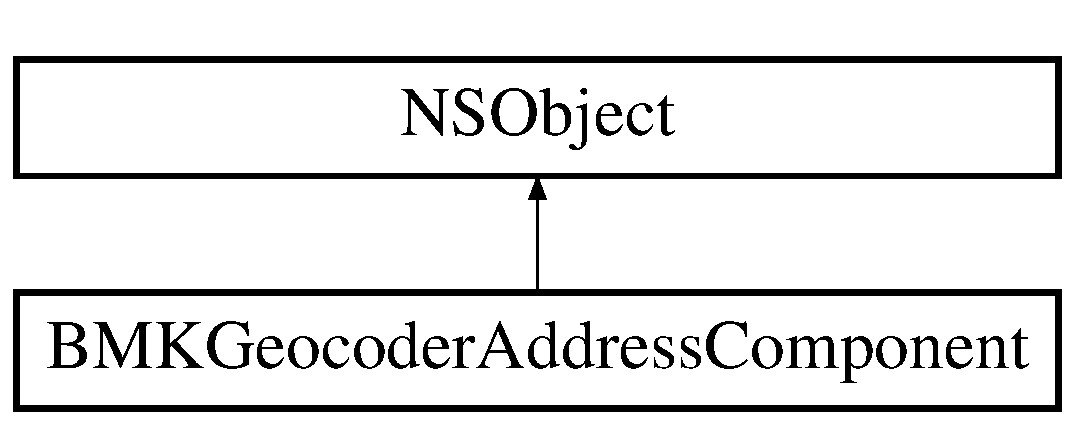
\includegraphics[height=2.000000cm]{interface_b_m_k_geocoder_address_component}
\end{center}
\end{figure}
\subsection*{保护成员变量}
\begin{DoxyCompactItemize}
\item 
\hypertarget{interface_b_m_k_geocoder_address_component_a7fd13ff466169fe05af2258e9f19db9b}{N\-S\-String $\ast$ {\bfseries \-\_\-street\-Number}}\label{interface_b_m_k_geocoder_address_component_a7fd13ff466169fe05af2258e9f19db9b}

\item 
\hypertarget{interface_b_m_k_geocoder_address_component_a971b3bc2bf3025aec31a9cc645ef8114}{N\-S\-String $\ast$ {\bfseries \-\_\-street\-Name}}\label{interface_b_m_k_geocoder_address_component_a971b3bc2bf3025aec31a9cc645ef8114}

\item 
\hypertarget{interface_b_m_k_geocoder_address_component_a66bc066e8337954449951c46c36623a7}{N\-S\-String $\ast$ {\bfseries \-\_\-district}}\label{interface_b_m_k_geocoder_address_component_a66bc066e8337954449951c46c36623a7}

\item 
\hypertarget{interface_b_m_k_geocoder_address_component_a70d4ba6d9ee3fa4ea21b2d7fba95a6fe}{N\-S\-String $\ast$ {\bfseries \-\_\-city}}\label{interface_b_m_k_geocoder_address_component_a70d4ba6d9ee3fa4ea21b2d7fba95a6fe}

\item 
\hypertarget{interface_b_m_k_geocoder_address_component_ad86b02dd1ac57bee274eb70f9421e1d9}{N\-S\-String $\ast$ {\bfseries \-\_\-province}}\label{interface_b_m_k_geocoder_address_component_ad86b02dd1ac57bee274eb70f9421e1d9}

\end{DoxyCompactItemize}
\subsection*{Properties}
\begin{DoxyCompactItemize}
\item 
\hypertarget{interface_b_m_k_geocoder_address_component_a76520d6c518cdab811f8ad7ffe4916bf}{N\-S\-String $\ast$ \hyperlink{interface_b_m_k_geocoder_address_component_a76520d6c518cdab811f8ad7ffe4916bf}{street\-Number}}\label{interface_b_m_k_geocoder_address_component_a76520d6c518cdab811f8ad7ffe4916bf}

\begin{DoxyCompactList}\small\item\em 街道号码 \end{DoxyCompactList}\item 
\hypertarget{interface_b_m_k_geocoder_address_component_a0d15f46f662c4ce8b47f411dab2a2be5}{N\-S\-String $\ast$ \hyperlink{interface_b_m_k_geocoder_address_component_a0d15f46f662c4ce8b47f411dab2a2be5}{street\-Name}}\label{interface_b_m_k_geocoder_address_component_a0d15f46f662c4ce8b47f411dab2a2be5}

\begin{DoxyCompactList}\small\item\em 街道名称 \end{DoxyCompactList}\item 
\hypertarget{interface_b_m_k_geocoder_address_component_a58897de3954b5a222cd76b7c8bbb901b}{N\-S\-String $\ast$ \hyperlink{interface_b_m_k_geocoder_address_component_a58897de3954b5a222cd76b7c8bbb901b}{district}}\label{interface_b_m_k_geocoder_address_component_a58897de3954b5a222cd76b7c8bbb901b}

\begin{DoxyCompactList}\small\item\em 区县名称 \end{DoxyCompactList}\item 
\hypertarget{interface_b_m_k_geocoder_address_component_ab5751bd3b4c34f1bac95a2a7dcba3197}{N\-S\-String $\ast$ \hyperlink{interface_b_m_k_geocoder_address_component_ab5751bd3b4c34f1bac95a2a7dcba3197}{city}}\label{interface_b_m_k_geocoder_address_component_ab5751bd3b4c34f1bac95a2a7dcba3197}

\begin{DoxyCompactList}\small\item\em 城市名称 \end{DoxyCompactList}\item 
\hypertarget{interface_b_m_k_geocoder_address_component_ae8b88f8a22f439069ad53049e5d7be36}{N\-S\-String $\ast$ \hyperlink{interface_b_m_k_geocoder_address_component_ae8b88f8a22f439069ad53049e5d7be36}{province}}\label{interface_b_m_k_geocoder_address_component_ae8b88f8a22f439069ad53049e5d7be36}

\begin{DoxyCompactList}\small\item\em 省份名称 \end{DoxyCompactList}\end{DoxyCompactItemize}


\subsection{详细描述}
此类表示地址结果的层次化信息 

The documentation for this class was generated from the following file\-:\begin{DoxyCompactItemize}
\item 
B\-M\-K\-Geocode\-Type.\-h\end{DoxyCompactItemize}

\hypertarget{struct_b_m_k_geo_point}{\section{B\-M\-K\-Geo\-Point Struct Reference}
\label{struct_b_m_k_geo_point}\index{B\-M\-K\-Geo\-Point@{B\-M\-K\-Geo\-Point}}
}


表示一个经纬度坐标点  




{\ttfamily \#include $<$B\-M\-K\-Geometry.\-h$>$}

\subsection*{公有成员变量}
\begin{DoxyCompactItemize}
\item 
\hypertarget{struct_b_m_k_geo_point_ad6f5b38335cff314e953e9b7eb5c7b39}{int \hyperlink{struct_b_m_k_geo_point_ad6f5b38335cff314e953e9b7eb5c7b39}{latitude\-E6}}\label{struct_b_m_k_geo_point_ad6f5b38335cff314e953e9b7eb5c7b39}

\begin{DoxyCompactList}\small\item\em 纬度,乘以1e6之后的值 \end{DoxyCompactList}\item 
\hypertarget{struct_b_m_k_geo_point_aac3f3dc0ae09785e5b70c319b68d4047}{int \hyperlink{struct_b_m_k_geo_point_aac3f3dc0ae09785e5b70c319b68d4047}{longitude\-E6}}\label{struct_b_m_k_geo_point_aac3f3dc0ae09785e5b70c319b68d4047}

\begin{DoxyCompactList}\small\item\em 经度,乘以1e6之后的值 \end{DoxyCompactList}\end{DoxyCompactItemize}


\subsection{详细描述}
表示一个经纬度坐标点 

The documentation for this struct was generated from the following file\-:\begin{DoxyCompactItemize}
\item 
\hyperlink{_b_m_k_geometry_8h}{B\-M\-K\-Geometry.\-h}\end{DoxyCompactItemize}

\hypertarget{interface_b_m_k_line}{\section{B\-M\-K\-Line 类参考}
\label{interface_b_m_k_line}\index{B\-M\-K\-Line@{B\-M\-K\-Line}}
}


公交路段结果类  




{\ttfamily \#import $<$B\-M\-K\-Route\-Search\-Type.\-h$>$}

继承关系图 B\-M\-K\-Line\-:\begin{figure}[H]
\begin{center}
\leavevmode
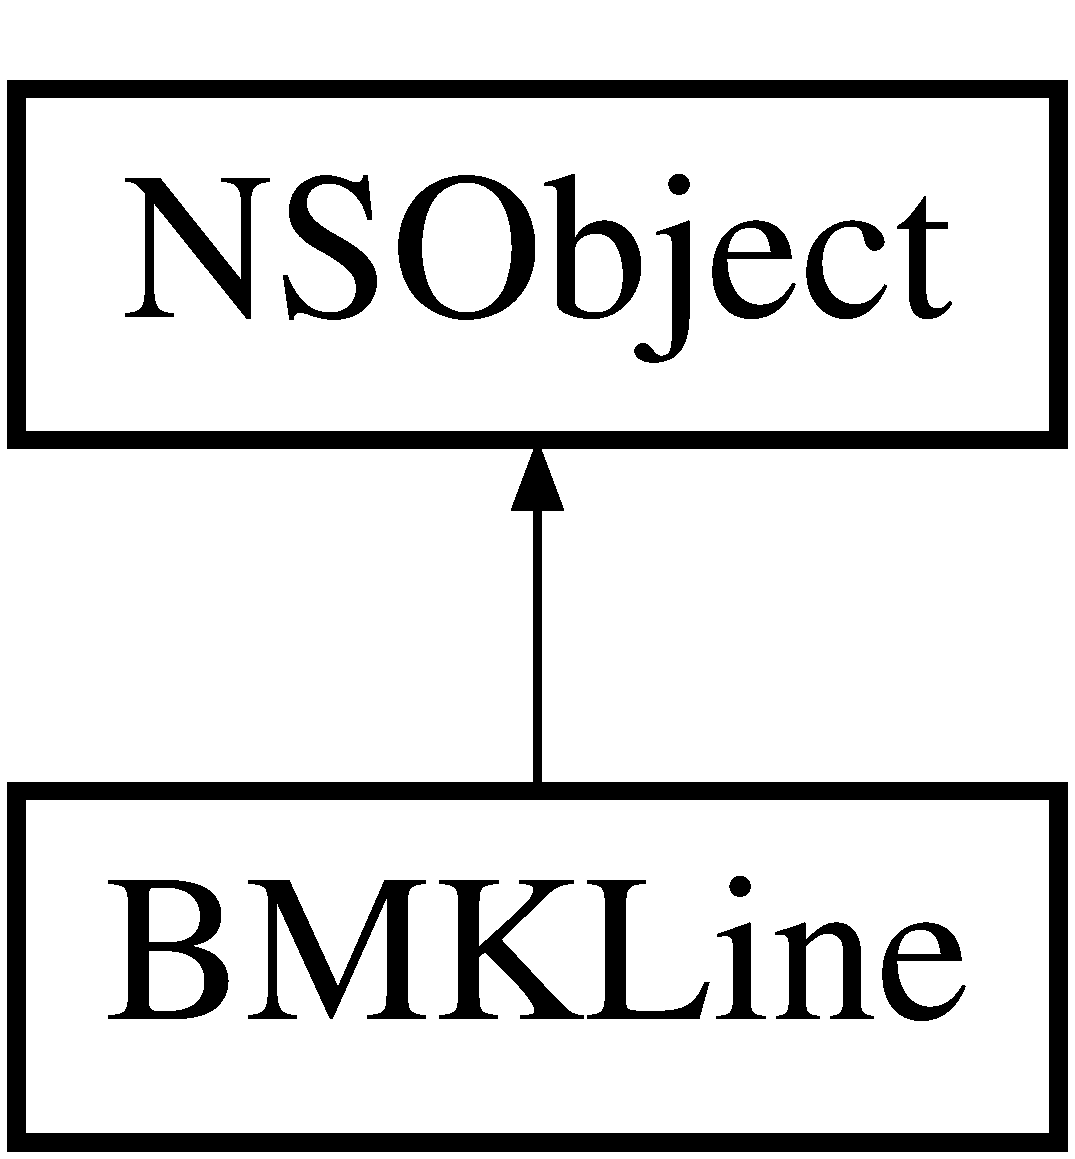
\includegraphics[height=2.000000cm]{interface_b_m_k_line}
\end{center}
\end{figure}
\subsection*{实例方法}
\begin{DoxyCompactItemize}
\item 
\hypertarget{interface_b_m_k_line_a33ce45bbba8d52b02ab9a8d01bcc29cf}{(\hyperlink{struct_b_m_k_map_point}{B\-M\-K\-Map\-Point} $\ast$) -\/ \hyperlink{interface_b_m_k_line_a33ce45bbba8d52b02ab9a8d01bcc29cf}{points}}\label{interface_b_m_k_line_a33ce45bbba8d52b02ab9a8d01bcc29cf}

\begin{DoxyCompactList}\small\item\em 线路坐标数组 \end{DoxyCompactList}\end{DoxyCompactItemize}
\subsection*{保护成员变量}
\begin{DoxyCompactItemize}
\item 
\hypertarget{interface_b_m_k_line_a2e7a14672b675d089fd2901295d25673}{int {\bfseries \-\_\-distance}}\label{interface_b_m_k_line_a2e7a14672b675d089fd2901295d25673}

\item 
\hypertarget{interface_b_m_k_line_a5fcb42fec4bf8715049776029312757c}{int {\bfseries \-\_\-type}}\label{interface_b_m_k_line_a5fcb42fec4bf8715049776029312757c}

\item 
\hypertarget{interface_b_m_k_line_ae029128ffc699ec5b89103a80343cc6c}{N\-S\-String $\ast$ {\bfseries \-\_\-title}}\label{interface_b_m_k_line_ae029128ffc699ec5b89103a80343cc6c}

\item 
\hypertarget{interface_b_m_k_line_ac24f2b082099c8b2cf6d8f4de06047dc}{N\-S\-String $\ast$ {\bfseries \-\_\-tip}}\label{interface_b_m_k_line_ac24f2b082099c8b2cf6d8f4de06047dc}

\item 
\hypertarget{interface_b_m_k_line_a50f2f33f1f170718e3e1e421c83b47cb}{\hyperlink{interface_b_m_k_poi_info}{B\-M\-K\-Poi\-Info} $\ast$ {\bfseries \-\_\-get\-On\-Stop\-Poi\-Info}}\label{interface_b_m_k_line_a50f2f33f1f170718e3e1e421c83b47cb}

\item 
\hypertarget{interface_b_m_k_line_a284c8a3e2d460bb47f53990b2f98fac4}{\hyperlink{interface_b_m_k_poi_info}{B\-M\-K\-Poi\-Info} $\ast$ {\bfseries \-\_\-get\-Off\-Stop\-Poi\-Info}}\label{interface_b_m_k_line_a284c8a3e2d460bb47f53990b2f98fac4}

\item 
\hypertarget{interface_b_m_k_line_a238759e096aa6b7fd31fb800a5baae7e}{\hyperlink{struct_b_m_k_map_point}{B\-M\-K\-Map\-Point} $\ast$ {\bfseries \-\_\-points}}\label{interface_b_m_k_line_a238759e096aa6b7fd31fb800a5baae7e}

\item 
\hypertarget{interface_b_m_k_line_ae85eada76152eedd34b6fb55f81bc21a}{int {\bfseries \-\_\-points\-Count}}\label{interface_b_m_k_line_ae85eada76152eedd34b6fb55f81bc21a}

\end{DoxyCompactItemize}
\subsection*{Properties}
\begin{DoxyCompactItemize}
\item 
\hypertarget{interface_b_m_k_line_a96b7d429c9f8a8b0d29aed3caf956f56}{int {\bfseries \-\_\-via\-Stops\-Num}}\label{interface_b_m_k_line_a96b7d429c9f8a8b0d29aed3caf956f56}

\item 
\hypertarget{interface_b_m_k_line_a0790fa0eb9e8f2d9db0d23e71a0af5d5}{int \hyperlink{interface_b_m_k_line_a0790fa0eb9e8f2d9db0d23e71a0af5d5}{via\-Stops\-Num}}\label{interface_b_m_k_line_a0790fa0eb9e8f2d9db0d23e71a0af5d5}

\begin{DoxyCompactList}\small\item\em 经过的公交站数 \end{DoxyCompactList}\item 
\hypertarget{interface_b_m_k_line_ab9d70d07678c78d4b34676b7b5eefc68}{int \hyperlink{interface_b_m_k_line_ab9d70d07678c78d4b34676b7b5eefc68}{distance}}\label{interface_b_m_k_line_ab9d70d07678c78d4b34676b7b5eefc68}

\begin{DoxyCompactList}\small\item\em 线路距离,单位:米 \end{DoxyCompactList}\item 
\hypertarget{interface_b_m_k_line_ac55c77014aabc4c4ff910246f41cac4d}{int \hyperlink{interface_b_m_k_line_ac55c77014aabc4c4ff910246f41cac4d}{type}}\label{interface_b_m_k_line_ac55c77014aabc4c4ff910246f41cac4d}

\begin{DoxyCompactList}\small\item\em 线路类型,0\-:公交 1\-:地铁 \end{DoxyCompactList}\item 
\hypertarget{interface_b_m_k_line_afb719a0a9ed606adc99a006ddb1daef8}{int \hyperlink{interface_b_m_k_line_afb719a0a9ed606adc99a006ddb1daef8}{points\-Count}}\label{interface_b_m_k_line_afb719a0a9ed606adc99a006ddb1daef8}

\begin{DoxyCompactList}\small\item\em 坐标点数目 \end{DoxyCompactList}\item 
\hypertarget{interface_b_m_k_line_af0af7177b41783fca20ed9d9af567ca0}{N\-S\-String $\ast$ \hyperlink{interface_b_m_k_line_af0af7177b41783fca20ed9d9af567ca0}{title}}\label{interface_b_m_k_line_af0af7177b41783fca20ed9d9af567ca0}

\begin{DoxyCompactList}\small\item\em 公交线路名称 \end{DoxyCompactList}\item 
\hypertarget{interface_b_m_k_line_a80154f88b4a14dcf2c4aedb966666a55}{N\-S\-String $\ast$ \hyperlink{interface_b_m_k_line_a80154f88b4a14dcf2c4aedb966666a55}{tip}}\label{interface_b_m_k_line_a80154f88b4a14dcf2c4aedb966666a55}

\begin{DoxyCompactList}\small\item\em 公交线路提示 \end{DoxyCompactList}\item 
\hypertarget{interface_b_m_k_line_a53866e3b80ad5a960932ca08a669d529}{\hyperlink{interface_b_m_k_poi_info}{B\-M\-K\-Poi\-Info} $\ast$ \hyperlink{interface_b_m_k_line_a53866e3b80ad5a960932ca08a669d529}{get\-On\-Stop\-Poi\-Info}}\label{interface_b_m_k_line_a53866e3b80ad5a960932ca08a669d529}

\begin{DoxyCompactList}\small\item\em 上车站点\-P\-O\-I信息 \end{DoxyCompactList}\item 
\hypertarget{interface_b_m_k_line_abb6b1b3baacc5038a187b0a36925ed50}{\hyperlink{interface_b_m_k_poi_info}{B\-M\-K\-Poi\-Info} $\ast$ \hyperlink{interface_b_m_k_line_abb6b1b3baacc5038a187b0a36925ed50}{get\-Off\-Stop\-Poi\-Info}}\label{interface_b_m_k_line_abb6b1b3baacc5038a187b0a36925ed50}

\begin{DoxyCompactList}\small\item\em 下车站点\-P\-O\-I信息 \end{DoxyCompactList}\end{DoxyCompactItemize}


\subsection{详细描述}
公交路段结果类 

The documentation for this class was generated from the following file\-:\begin{DoxyCompactItemize}
\item 
B\-M\-K\-Route\-Search\-Type.\-h\end{DoxyCompactItemize}

\hypertarget{interface_b_m_k_map_manager}{\section{B\-M\-K\-Map\-Manager 类参考}
\label{interface_b_m_k_map_manager}\index{B\-M\-K\-Map\-Manager@{B\-M\-K\-Map\-Manager}}
}


主引擎类  




{\ttfamily \#import $<$B\-M\-K\-Map\-Manager.\-h$>$}

继承关系图 B\-M\-K\-Map\-Manager\-:\begin{figure}[H]
\begin{center}
\leavevmode
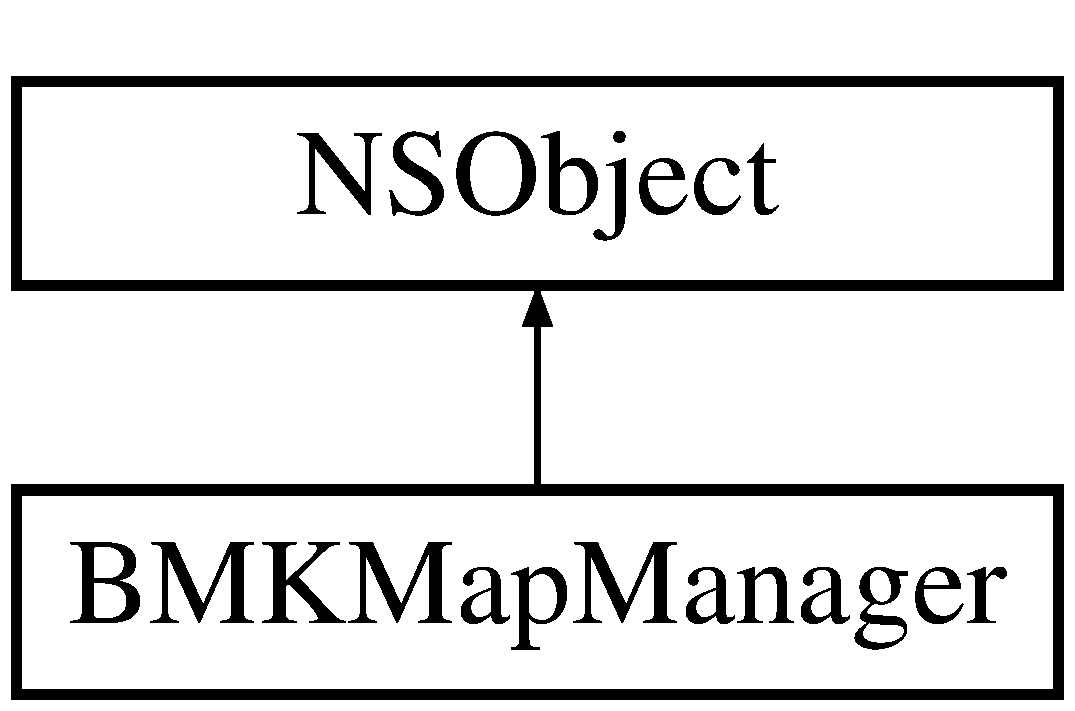
\includegraphics[height=2.000000cm]{interface_b_m_k_map_manager}
\end{center}
\end{figure}
\subsection*{实例方法}
\begin{DoxyCompactItemize}
\item 
(B\-O\-O\-L) -\/ \hyperlink{interface_b_m_k_map_manager_a95edf9c8fea4c61a79098641c4e9a50f}{start\-:general\-Delegate\-:}
\item 
(B\-O\-O\-L) -\/ \hyperlink{interface_b_m_k_map_manager_ac53850202f5017ff35c8933c171be0f1}{stop}
\end{DoxyCompactItemize}


\subsection{详细描述}
主引擎类 

\subsection{方法文档}
\hypertarget{interface_b_m_k_map_manager_a95edf9c8fea4c61a79098641c4e9a50f}{\index{B\-M\-K\-Map\-Manager@{B\-M\-K\-Map\-Manager}!start\-:general\-Delegate\-:@{start\-:general\-Delegate\-:}}
\index{start\-:general\-Delegate\-:@{start\-:general\-Delegate\-:}!BMKMapManager@{B\-M\-K\-Map\-Manager}}
\subsubsection[{start\-:general\-Delegate\-:}]{\setlength{\rightskip}{0pt plus 5cm}-\/ (B\-O\-O\-L) start\-: 
\begin{DoxyParamCaption}
\item[{(N\-S\-String $\ast$)}]{key}
\item[{generalDelegate:(id$<$ {\bf B\-M\-K\-General\-Delegate} $>$)}]{delegate}
\end{DoxyParamCaption}
}}\label{interface_b_m_k_map_manager_a95edf9c8fea4c61a79098641c4e9a50f}
启动引擎 
\begin{DoxyParams}{参数}
{\em key} & 申请的有效key \\
\hline
{\em delegate} & \\
\hline
\end{DoxyParams}
\hypertarget{interface_b_m_k_map_manager_ac53850202f5017ff35c8933c171be0f1}{\index{B\-M\-K\-Map\-Manager@{B\-M\-K\-Map\-Manager}!stop@{stop}}
\index{stop@{stop}!BMKMapManager@{B\-M\-K\-Map\-Manager}}
\subsubsection[{stop}]{\setlength{\rightskip}{0pt plus 5cm}-\/ (B\-O\-O\-L) stop 
\begin{DoxyParamCaption}
{}
\end{DoxyParamCaption}
}}\label{interface_b_m_k_map_manager_ac53850202f5017ff35c8933c171be0f1}
停止引擎 

The documentation for this class was generated from the following file\-:\begin{DoxyCompactItemize}
\item 
B\-M\-K\-Map\-Manager.\-h\end{DoxyCompactItemize}

\hypertarget{interface_b_m_k_map_poi}{\section{B\-M\-K\-Map\-Poi 类参考}
\label{interface_b_m_k_map_poi}\index{B\-M\-K\-Map\-Poi@{B\-M\-K\-Map\-Poi}}
}


点击地图标注返回数据结构  




{\ttfamily \#import $<$B\-M\-K\-Map\-View.\-h$>$}

继承关系图 B\-M\-K\-Map\-Poi\-:\begin{figure}[H]
\begin{center}
\leavevmode
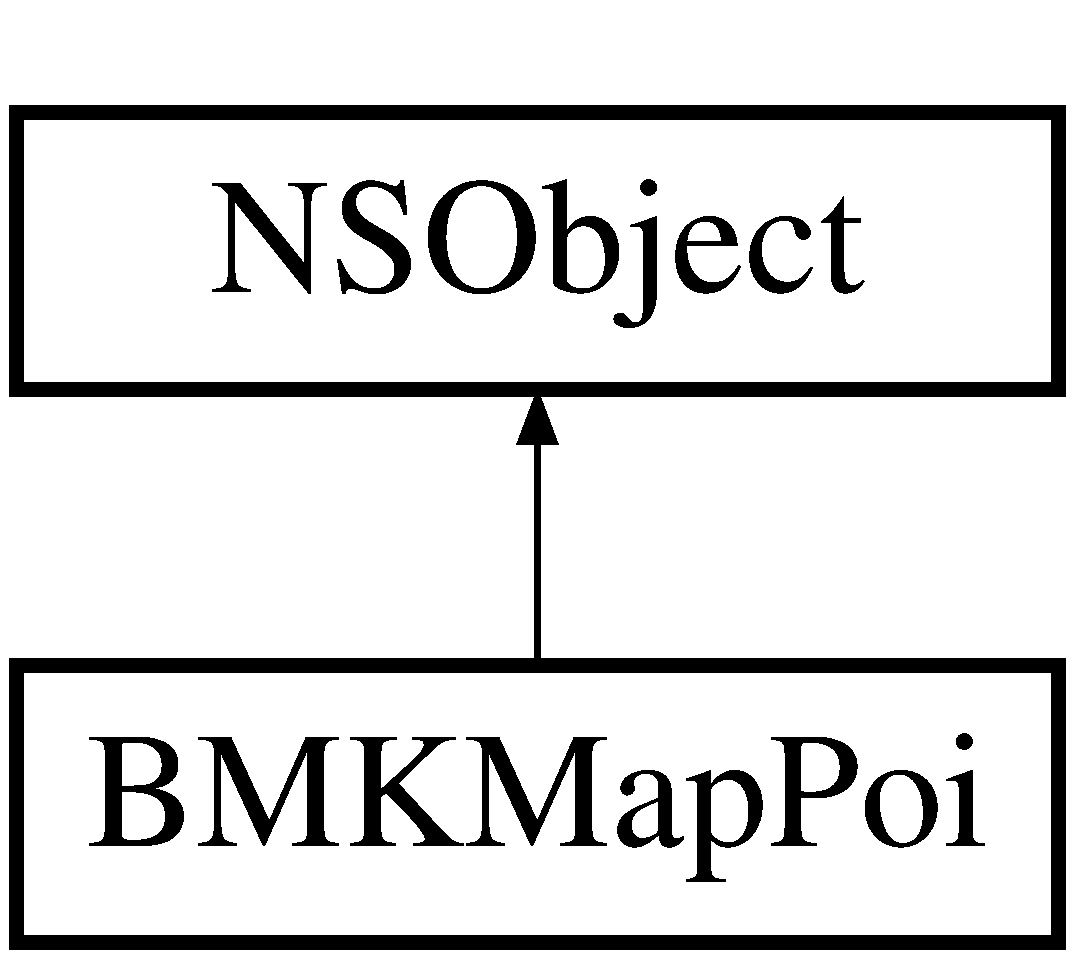
\includegraphics[height=2.000000cm]{interface_b_m_k_map_poi}
\end{center}
\end{figure}
\subsection*{Properties}
\begin{DoxyCompactItemize}
\item 
\hypertarget{interface_b_m_k_map_poi_a5d5c19bd352dcab43167d97aa47ea38d}{N\-S\-String $\ast$ \hyperlink{interface_b_m_k_map_poi_a5d5c19bd352dcab43167d97aa47ea38d}{text}}\label{interface_b_m_k_map_poi_a5d5c19bd352dcab43167d97aa47ea38d}

\begin{DoxyCompactList}\small\item\em 点标注的名称 \end{DoxyCompactList}\item 
\hypertarget{interface_b_m_k_map_poi_a771c0672bbe2dd1dc526003717bbcec1}{C\-L\-Location\-Coordinate2\-D \hyperlink{interface_b_m_k_map_poi_a771c0672bbe2dd1dc526003717bbcec1}{pt}}\label{interface_b_m_k_map_poi_a771c0672bbe2dd1dc526003717bbcec1}

\begin{DoxyCompactList}\small\item\em 点标注的经纬度坐标 \end{DoxyCompactList}\end{DoxyCompactItemize}


\subsection{详细描述}
点击地图标注返回数据结构 

The documentation for this class was generated from the following file\-:\begin{DoxyCompactItemize}
\item 
B\-M\-K\-Map\-View.\-h\end{DoxyCompactItemize}

\hypertarget{struct_b_m_k_map_point}{\section{B\-M\-K\-Map\-Point Struct Reference}
\label{struct_b_m_k_map_point}\index{B\-M\-K\-Map\-Point@{B\-M\-K\-Map\-Point}}
}


地理坐标点,用直角地理坐标表示  




{\ttfamily \#include $<$B\-M\-K\-Geometry.\-h$>$}

\subsection*{公有成员变量}
\begin{DoxyCompactItemize}
\item 
\hypertarget{struct_b_m_k_map_point_a8c0ca1c3f0cbb5fe183ae7745781d8fb}{double \hyperlink{struct_b_m_k_map_point_a8c0ca1c3f0cbb5fe183ae7745781d8fb}{x}}\label{struct_b_m_k_map_point_a8c0ca1c3f0cbb5fe183ae7745781d8fb}

\begin{DoxyCompactList}\small\item\em 横坐标 \end{DoxyCompactList}\item 
\hypertarget{struct_b_m_k_map_point_a9d0aff0bad009459af85d1e51a194341}{double \hyperlink{struct_b_m_k_map_point_a9d0aff0bad009459af85d1e51a194341}{y}}\label{struct_b_m_k_map_point_a9d0aff0bad009459af85d1e51a194341}

\begin{DoxyCompactList}\small\item\em 纵坐标 \end{DoxyCompactList}\end{DoxyCompactItemize}


\subsection{详细描述}
地理坐标点,用直角地理坐标表示 

The documentation for this struct was generated from the following file\-:\begin{DoxyCompactItemize}
\item 
\hyperlink{_b_m_k_geometry_8h}{B\-M\-K\-Geometry.\-h}\end{DoxyCompactItemize}

\hypertarget{struct_b_m_k_map_rect}{\section{B\-M\-K\-Map\-Rect Struct Reference}
\label{struct_b_m_k_map_rect}\index{B\-M\-K\-Map\-Rect@{B\-M\-K\-Map\-Rect}}
}


矩形,用直角地理坐标表示  




{\ttfamily \#include $<$B\-M\-K\-Geometry.\-h$>$}

\subsection*{公有成员变量}
\begin{DoxyCompactItemize}
\item 
\hypertarget{struct_b_m_k_map_rect_aeeee8bcaabf5c65e222f1891009325f1}{\hyperlink{struct_b_m_k_map_point}{B\-M\-K\-Map\-Point} \hyperlink{struct_b_m_k_map_rect_aeeee8bcaabf5c65e222f1891009325f1}{origin}}\label{struct_b_m_k_map_rect_aeeee8bcaabf5c65e222f1891009325f1}

\begin{DoxyCompactList}\small\item\em 屏幕左上点对应的直角地理坐标 \end{DoxyCompactList}\item 
\hypertarget{struct_b_m_k_map_rect_ab83b0fb9e6e63b6ab24bdce9ced1e92e}{\hyperlink{struct_b_m_k_map_size}{B\-M\-K\-Map\-Size} \hyperlink{struct_b_m_k_map_rect_ab83b0fb9e6e63b6ab24bdce9ced1e92e}{size}}\label{struct_b_m_k_map_rect_ab83b0fb9e6e63b6ab24bdce9ced1e92e}

\begin{DoxyCompactList}\small\item\em 坐标范围 \end{DoxyCompactList}\end{DoxyCompactItemize}


\subsection{详细描述}
矩形,用直角地理坐标表示 

The documentation for this struct was generated from the following file\-:\begin{DoxyCompactItemize}
\item 
\hyperlink{_b_m_k_geometry_8h}{B\-M\-K\-Geometry.\-h}\end{DoxyCompactItemize}

\hypertarget{struct_b_m_k_map_size}{\section{B\-M\-K\-Map\-Size Struct Reference}
\label{struct_b_m_k_map_size}\index{B\-M\-K\-Map\-Size@{B\-M\-K\-Map\-Size}}
}


矩形大小,用直角地理坐标表示  




{\ttfamily \#include $<$B\-M\-K\-Geometry.\-h$>$}

\subsection*{公有成员变量}
\begin{DoxyCompactItemize}
\item 
\hypertarget{struct_b_m_k_map_size_a1005d7fd59045a80619c024df3156d6a}{double \hyperlink{struct_b_m_k_map_size_a1005d7fd59045a80619c024df3156d6a}{width}}\label{struct_b_m_k_map_size_a1005d7fd59045a80619c024df3156d6a}

\begin{DoxyCompactList}\small\item\em 宽度 \end{DoxyCompactList}\item 
\hypertarget{struct_b_m_k_map_size_a516baff78187bf8f07ef49f01c7d86fc}{double \hyperlink{struct_b_m_k_map_size_a516baff78187bf8f07ef49f01c7d86fc}{height}}\label{struct_b_m_k_map_size_a516baff78187bf8f07ef49f01c7d86fc}

\begin{DoxyCompactList}\small\item\em 高度 \end{DoxyCompactList}\end{DoxyCompactItemize}


\subsection{详细描述}
矩形大小,用直角地理坐标表示 

The documentation for this struct was generated from the following file\-:\begin{DoxyCompactItemize}
\item 
\hyperlink{_b_m_k_geometry_8h}{B\-M\-K\-Geometry.\-h}\end{DoxyCompactItemize}

\hypertarget{interface_b_m_k_map_view}{\section{B\-M\-K\-Map\-View 类参考}
\label{interface_b_m_k_map_view}\index{B\-M\-K\-Map\-View@{B\-M\-K\-Map\-View}}
}


地图\-View类,使用此\-View可以显示地图窗口,并且对地图进行相关的操作  




{\ttfamily \#import $<$B\-M\-K\-Map\-View.\-h$>$}

继承关系图 B\-M\-K\-Map\-View\-:\begin{figure}[H]
\begin{center}
\leavevmode
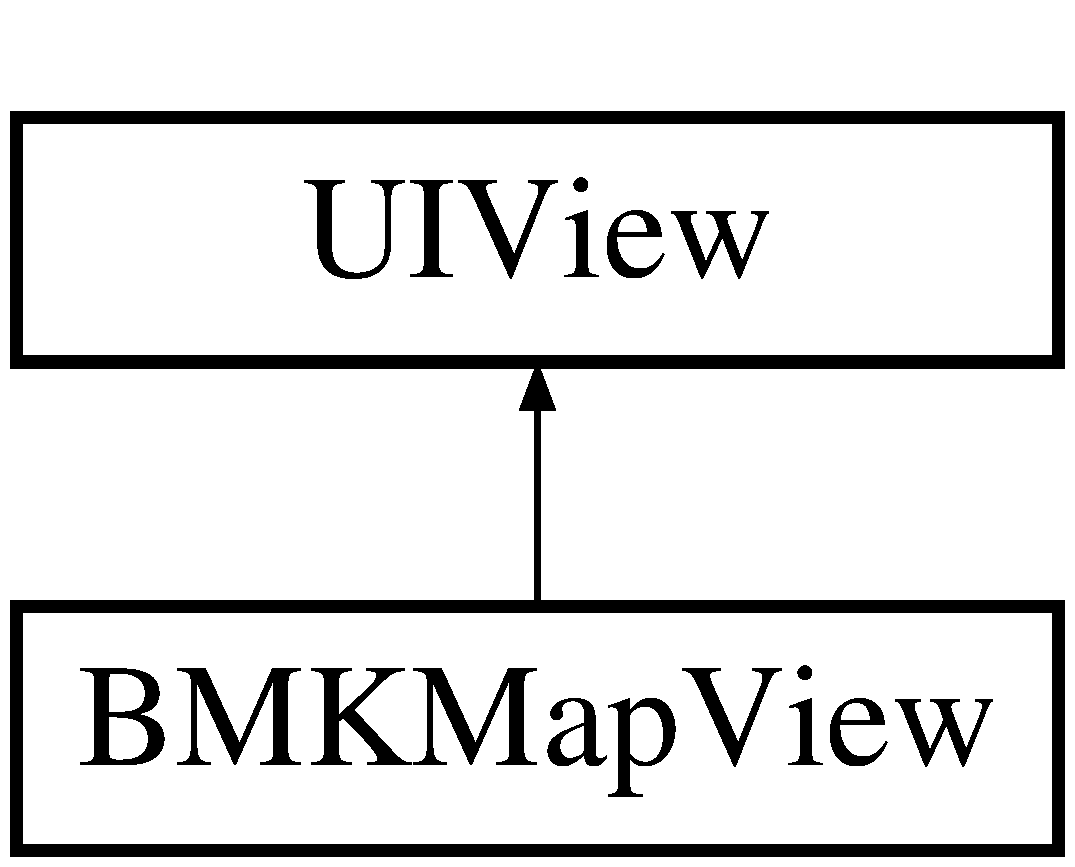
\includegraphics[height=2.000000cm]{interface_b_m_k_map_view}
\end{center}
\end{figure}
\subsection*{实例方法}
\begin{DoxyCompactItemize}
\item 
(void) -\/ \hyperlink{interface_b_m_k_map_view_af182240990fe7ad8ff8b709456200fed}{set\-Region\-:animated\-:}
\item 
(void) -\/ \hyperlink{interface_b_m_k_map_view_a02c0933bb56354f30695a6634e416e26}{set\-Center\-Coordinate\-:animated\-:}
\item 
(void) -\/ \hyperlink{interface_b_m_k_map_view_a6ce8ac560bd901b93b3e15d6996a409a}{view\-Will\-Appear}
\item 
(void) -\/ \hyperlink{interface_b_m_k_map_view_a0cfbfc217062e84de41ddb04dcad7e67}{view\-Will\-Disappear}
\item 
(B\-O\-O\-L) -\/ \hyperlink{interface_b_m_k_map_view_a349f7c74871a389d73955edd7bcd9fdf}{zoom\-In}
\item 
(B\-O\-O\-L) -\/ \hyperlink{interface_b_m_k_map_view_a1806c818757917ef674ebe5ba24fe5a2}{zoom\-Out}
\item 
(\hyperlink{struct_b_m_k_coordinate_region}{B\-M\-K\-Coordinate\-Region}) -\/ \hyperlink{interface_b_m_k_map_view_a5a1387f64868bf341cbf743063a91d28}{region\-That\-Fits\-:}
\item 
(U\-I\-Image $\ast$) -\/ \hyperlink{interface_b_m_k_map_view_af2af641b86f327aa9f2a16050d380db2}{take\-Snapshot}
\item 
(void) -\/ \hyperlink{interface_b_m_k_map_view_ad90d3e9ceabed218dcb90d9fc8247902}{set\-Visible\-Map\-Rect\-:animated\-:}
\item 
(\hyperlink{struct_b_m_k_map_rect}{B\-M\-K\-Map\-Rect}) -\/ \hyperlink{interface_b_m_k_map_view_a58f9c0d783d39cd0d028ae94ca408de8}{map\-Rect\-That\-Fits\-:}
\item 
(void) -\/ \hyperlink{interface_b_m_k_map_view_a1e5a69629b90ac2f571284e2e6c32397}{set\-Visible\-Map\-Rect\-:edge\-Padding\-:animated\-:}
\item 
(\hyperlink{struct_b_m_k_map_rect}{B\-M\-K\-Map\-Rect}) -\/ \hyperlink{interface_b_m_k_map_view_a93e07fbbe602a9a493650158babd2349}{map\-Rect\-That\-Fits\-:edge\-Padding\-:}
\item 
(C\-G\-Point) -\/ \hyperlink{interface_b_m_k_map_view_a46ec1b9f485f41a04ffe76300624f5b4}{convert\-Coordinate\-:to\-Point\-To\-View\-:}
\item 
(C\-L\-Location\-Coordinate2\-D) -\/ \hyperlink{interface_b_m_k_map_view_a6ab0dbfdf28bf2ab29174d9a70ce2e9c}{convert\-Point\-:to\-Coordinate\-From\-View\-:}
\item 
(C\-G\-Rect) -\/ \hyperlink{interface_b_m_k_map_view_a952023c2e24a13c993977d276745f329}{convert\-Region\-:to\-Rect\-To\-View\-:}
\item 
(\hyperlink{struct_b_m_k_coordinate_region}{B\-M\-K\-Coordinate\-Region}) -\/ \hyperlink{interface_b_m_k_map_view_ae99130c0eceabae6c9e202699ba375d1}{convert\-Rect\-:to\-Region\-From\-View\-:}
\item 
(C\-G\-Rect) -\/ \hyperlink{interface_b_m_k_map_view_a4a802244887690c7238bd5c8e18918ae}{convert\-Map\-Rect\-:to\-Rect\-To\-View\-:}
\item 
(\hyperlink{struct_b_m_k_map_rect}{B\-M\-K\-Map\-Rect}) -\/ \hyperlink{interface_b_m_k_map_view_afa77dab84c13620c4ce0dee46df87b46}{convert\-Rect\-:to\-Map\-Rect\-From\-View\-:}
\item 
(void) -\/ \hyperlink{interface_b_m_k_map_view_a1bf0349f0eb4580ca23eac1032345925}{add\-Annotation\-:}
\item 
(void) -\/ \hyperlink{interface_b_m_k_map_view_ad863c0ccb09937907188a408103f8234}{add\-Annotations\-:}
\item 
(void) -\/ \hyperlink{interface_b_m_k_map_view_a5a6efcf38e824c225c8dc3132edb4c02}{remove\-Annotation\-:}
\item 
(void) -\/ \hyperlink{interface_b_m_k_map_view_aa3cccccb36e36704debcdeb0093559f2}{remove\-Annotations\-:}
\item 
(\hyperlink{interface_b_m_k_annotation_view}{B\-M\-K\-Annotation\-View} $\ast$) -\/ \hyperlink{interface_b_m_k_map_view_ac93853efa99f78f20cc2b260bc734511}{view\-For\-Annotation\-:}
\item 
(\hyperlink{interface_b_m_k_annotation_view}{B\-M\-K\-Annotation\-View} $\ast$) -\/ \hyperlink{interface_b_m_k_map_view_a295564a4e2ed533a7ba2fc9f0fe3c008}{dequeue\-Reusable\-Annotation\-View\-With\-Identifier\-:}
\item 
(void) -\/ \hyperlink{interface_b_m_k_map_view_a9b26d1286a51cf260bea06d8ed220316}{select\-Annotation\-:animated\-:}
\item 
(void) -\/ \hyperlink{interface_b_m_k_map_view_a8d2f82aae2c0a536c057239442573fb2}{deselect\-Annotation\-:animated\-:}
\item 
(void) -\/ \hyperlink{interface_b_m_k_map_view_af85ad6091568df29d9e7c3dea82a1a2b}{add\-Overlay\-:}
\item 
(void) -\/ \hyperlink{interface_b_m_k_map_view_ab7d29d948515cc6d947d6aa63f904168}{add\-Overlays\-:}
\item 
(void) -\/ \hyperlink{interface_b_m_k_map_view_a3be1f2a019df3ff971f6a36f142e55be}{remove\-Overlay\-:}
\item 
(void) -\/ \hyperlink{interface_b_m_k_map_view_a3eb7909fb1adce117c1de432fd5d816a}{remove\-Overlays\-:}
\item 
(void) -\/ \hyperlink{interface_b_m_k_map_view_adc0775a2651c1e4099f93d9c1bbffe3d}{insert\-Overlay\-:at\-Index\-:}
\item 
(void) -\/ \hyperlink{interface_b_m_k_map_view_a62c1c29b8e5b408ba0c40411a3c1f50f}{exchange\-Overlay\-At\-Index\-:with\-Overlay\-At\-Index\-:}
\item 
(void) -\/ \hyperlink{interface_b_m_k_map_view_ad94b45c4df7978e3a6095918323496d3}{insert\-Overlay\-:above\-Overlay\-:}
\item 
(void) -\/ \hyperlink{interface_b_m_k_map_view_a73dfe9f74d722b7b1fc477e791f34653}{insert\-Overlay\-:below\-Overlay\-:}
\item 
(\hyperlink{interface_b_m_k_overlay_view}{B\-M\-K\-Overlay\-View} $\ast$) -\/ \hyperlink{interface_b_m_k_map_view_aa88093440ad22f7af9cf9a36051f662d}{view\-For\-Overlay\-:}
\end{DoxyCompactItemize}
\subsection*{Properties}
\begin{DoxyCompactItemize}
\item 
\hypertarget{interface_b_m_k_map_view_a80806d05b9f82dcf5630110b5d20dc2c}{id$<$ \hyperlink{protocol_b_m_k_map_view_delegate-p}{B\-M\-K\-Map\-View\-Delegate} $>$ \hyperlink{interface_b_m_k_map_view_a80806d05b9f82dcf5630110b5d20dc2c}{delegate}}\label{interface_b_m_k_map_view_a80806d05b9f82dcf5630110b5d20dc2c}

\begin{DoxyCompactList}\small\item\em 地图\-View的\-Delegate,此处记得不用的时候需要置nil,否则影响内存的释放 \end{DoxyCompactList}\item 
\hypertarget{interface_b_m_k_map_view_add5778e2d3c080b0ae2ce63538082fea}{B\-M\-K\-Map\-Type \hyperlink{interface_b_m_k_map_view_add5778e2d3c080b0ae2ce63538082fea}{map\-Type}}\label{interface_b_m_k_map_view_add5778e2d3c080b0ae2ce63538082fea}

\begin{DoxyCompactList}\small\item\em 当前地图类型,可设定为标准地图、实时路况、卫星地图、同时打开实时路况和卫星地图模式 \end{DoxyCompactList}\item 
\hypertarget{interface_b_m_k_map_view_ae54e847bb82b4e087ced8dc399a2d020}{\hyperlink{struct_b_m_k_coordinate_region}{B\-M\-K\-Coordinate\-Region} \hyperlink{interface_b_m_k_map_view_ae54e847bb82b4e087ced8dc399a2d020}{region}}\label{interface_b_m_k_map_view_ae54e847bb82b4e087ced8dc399a2d020}

\begin{DoxyCompactList}\small\item\em 当前地图的经纬度范围,设定的该范围可能会被调整为适合地图窗口显示的范围 \end{DoxyCompactList}\item 
\hypertarget{interface_b_m_k_map_view_adad44db2dcfaa2d92e5eabef40f32bd8}{C\-G\-Point \hyperlink{interface_b_m_k_map_view_adad44db2dcfaa2d92e5eabef40f32bd8}{compass\-Position}}\label{interface_b_m_k_map_view_adad44db2dcfaa2d92e5eabef40f32bd8}

\begin{DoxyCompactList}\small\item\em 指南针的位置,设定坐标以\-B\-M\-K\-Map\-View左上角为原点,向右向下增长 \end{DoxyCompactList}\item 
\hypertarget{interface_b_m_k_map_view_aa19c4d034a7861589044326107985632}{C\-L\-Location\-Coordinate2\-D \hyperlink{interface_b_m_k_map_view_aa19c4d034a7861589044326107985632}{center\-Coordinate}}\label{interface_b_m_k_map_view_aa19c4d034a7861589044326107985632}

\begin{DoxyCompactList}\small\item\em 当前地图的中心点,改变该值时,地图的比例尺级别不会发生变化 \end{DoxyCompactList}\item 
\hypertarget{interface_b_m_k_map_view_a5e6c1e21fddd4d6a24194be53f14c27e}{float \hyperlink{interface_b_m_k_map_view_a5e6c1e21fddd4d6a24194be53f14c27e}{zoom\-Level}}\label{interface_b_m_k_map_view_a5e6c1e21fddd4d6a24194be53f14c27e}

\begin{DoxyCompactList}\small\item\em 地图比例尺级别,在手机上当前可使用的级别为3-\/19级 \end{DoxyCompactList}\item 
\hypertarget{interface_b_m_k_map_view_a344d3d4be5d00adfc22feaa2ab6869c4}{int \hyperlink{interface_b_m_k_map_view_a344d3d4be5d00adfc22feaa2ab6869c4}{rotation}}\label{interface_b_m_k_map_view_a344d3d4be5d00adfc22feaa2ab6869c4}

\begin{DoxyCompactList}\small\item\em 地图旋转角度,在手机上当前可使用的范围为-180~180度 \end{DoxyCompactList}\item 
\hypertarget{interface_b_m_k_map_view_a8ae6f6cf221ea4f14923150d8974f997}{int \hyperlink{interface_b_m_k_map_view_a8ae6f6cf221ea4f14923150d8974f997}{overlooking}}\label{interface_b_m_k_map_view_a8ae6f6cf221ea4f14923150d8974f997}

\begin{DoxyCompactList}\small\item\em 地图俯视角度,在手机上当前可使用的范围为-45~0度 \end{DoxyCompactList}\item 
\hypertarget{interface_b_m_k_map_view_af0b1358b03cf2e760d58c96dc50d3ebe}{B\-O\-O\-L \hyperlink{interface_b_m_k_map_view_af0b1358b03cf2e760d58c96dc50d3ebe}{shows\-User\-Location}}\label{interface_b_m_k_map_view_af0b1358b03cf2e760d58c96dc50d3ebe}

\begin{DoxyCompactList}\small\item\em 设定是否显示定位图层 \end{DoxyCompactList}\item 
\hypertarget{interface_b_m_k_map_view_a165690d8952edbf58fd33101d3d169e8}{\hyperlink{interface_b_m_k_user_location}{B\-M\-K\-User\-Location} $\ast$ \hyperlink{interface_b_m_k_map_view_a165690d8952edbf58fd33101d3d169e8}{user\-Location}}\label{interface_b_m_k_map_view_a165690d8952edbf58fd33101d3d169e8}

\begin{DoxyCompactList}\small\item\em 当前用户位置,返回坐标为百度坐标 \end{DoxyCompactList}\item 
\hypertarget{interface_b_m_k_map_view_a8e3facab242ecd1ea2aadea90c158b99}{B\-O\-O\-L \hyperlink{interface_b_m_k_map_view_a8e3facab242ecd1ea2aadea90c158b99}{user\-Location\-Visible}}\label{interface_b_m_k_map_view_a8e3facab242ecd1ea2aadea90c158b99}

\begin{DoxyCompactList}\small\item\em 返回定位坐标点是否在当前地图可视区域内 \end{DoxyCompactList}\item 
\hypertarget{interface_b_m_k_map_view_a35576ab39592ef50d1190c2b672c0923}{\hyperlink{struct_b_m_k_map_rect}{B\-M\-K\-Map\-Rect} \hyperlink{interface_b_m_k_map_view_a35576ab39592ef50d1190c2b672c0923}{visible\-Map\-Rect}}\label{interface_b_m_k_map_view_a35576ab39592ef50d1190c2b672c0923}

\begin{DoxyCompactList}\small\item\em 当前地图范围,采用直角坐标系表示,向右向下增长 \end{DoxyCompactList}\item 
\hypertarget{interface_b_m_k_map_view_acf8472da994b76cef21a40673a41f774}{B\-O\-O\-L \hyperlink{interface_b_m_k_map_view_acf8472da994b76cef21a40673a41f774}{zoom\-Enabled}}\label{interface_b_m_k_map_view_acf8472da994b76cef21a40673a41f774}

\begin{DoxyCompactList}\small\item\em 设定地图\-View能否支持用户多点缩放 \end{DoxyCompactList}\item 
\hypertarget{interface_b_m_k_map_view_adc7ae3120b0edf096ac0eb42f13ed93a}{B\-O\-O\-L \hyperlink{interface_b_m_k_map_view_adc7ae3120b0edf096ac0eb42f13ed93a}{scroll\-Enabled}}\label{interface_b_m_k_map_view_adc7ae3120b0edf096ac0eb42f13ed93a}

\begin{DoxyCompactList}\small\item\em 设定地图\-View能否支持用户移动地图 \end{DoxyCompactList}\item 
\hypertarget{interface_b_m_k_map_view_a4d6a0d91974378d36f8da982e3eb85e8}{N\-S\-Array $\ast$ \hyperlink{interface_b_m_k_map_view_a4d6a0d91974378d36f8da982e3eb85e8}{annotations}}\label{interface_b_m_k_map_view_a4d6a0d91974378d36f8da982e3eb85e8}

\begin{DoxyCompactList}\small\item\em 当前地图\-View的已经添加的标注数组 \end{DoxyCompactList}\item 
\hypertarget{interface_b_m_k_map_view_a6c673c46ad9f146f80e48d82ebcf934b}{N\-S\-Array $\ast$ \hyperlink{interface_b_m_k_map_view_a6c673c46ad9f146f80e48d82ebcf934b}{overlays}}\label{interface_b_m_k_map_view_a6c673c46ad9f146f80e48d82ebcf934b}

\begin{DoxyCompactList}\small\item\em 当前map\-View中已经添加的\-Overlay数组 \end{DoxyCompactList}\end{DoxyCompactItemize}


\subsection{详细描述}
地图\-View类,使用此\-View可以显示地图窗口,并且对地图进行相关的操作 

\subsection{方法文档}
\hypertarget{interface_b_m_k_map_view_a1bf0349f0eb4580ca23eac1032345925}{\index{B\-M\-K\-Map\-View@{B\-M\-K\-Map\-View}!add\-Annotation\-:@{add\-Annotation\-:}}
\index{add\-Annotation\-:@{add\-Annotation\-:}!BMKMapView@{B\-M\-K\-Map\-View}}
\subsubsection[{add\-Annotation\-:}]{\setlength{\rightskip}{0pt plus 5cm}-\/ (void) add\-Annotation\-: 
\begin{DoxyParamCaption}
\item[{(id$<$ {\bf B\-M\-K\-Annotation} $>$)}]{annotation}
\end{DoxyParamCaption}
}}\label{interface_b_m_k_map_view_a1bf0349f0eb4580ca23eac1032345925}
向地图窗口添加标注,需要实现\-B\-M\-K\-Map\-View\-Delegate的-\/map\-View\-:view\-For\-Annotation\-:函数来生成标注对应的\-View 
\begin{DoxyParams}{参数}
{\em annotation} & 要添加的标注 \\
\hline
\end{DoxyParams}
\hypertarget{interface_b_m_k_map_view_ad863c0ccb09937907188a408103f8234}{\index{B\-M\-K\-Map\-View@{B\-M\-K\-Map\-View}!add\-Annotations\-:@{add\-Annotations\-:}}
\index{add\-Annotations\-:@{add\-Annotations\-:}!BMKMapView@{B\-M\-K\-Map\-View}}
\subsubsection[{add\-Annotations\-:}]{\setlength{\rightskip}{0pt plus 5cm}-\/ (void) add\-Annotations\-: 
\begin{DoxyParamCaption}
\item[{(N\-S\-Array $\ast$)}]{annotations}
\end{DoxyParamCaption}
}}\label{interface_b_m_k_map_view_ad863c0ccb09937907188a408103f8234}
向地图窗口添加一组标注,需要实现\-B\-M\-K\-Map\-View\-Delegate的-\/map\-View\-:view\-For\-Annotation\-:函数来生成标注对应的\-View 
\begin{DoxyParams}{参数}
{\em annotations} & 要添加的标注数组 \\
\hline
\end{DoxyParams}
\hypertarget{interface_b_m_k_map_view_af85ad6091568df29d9e7c3dea82a1a2b}{\index{B\-M\-K\-Map\-View@{B\-M\-K\-Map\-View}!add\-Overlay\-:@{add\-Overlay\-:}}
\index{add\-Overlay\-:@{add\-Overlay\-:}!BMKMapView@{B\-M\-K\-Map\-View}}
\subsubsection[{add\-Overlay\-:}]{\setlength{\rightskip}{0pt plus 5cm}-\/ (void) add\-Overlay\-: 
\begin{DoxyParamCaption}
\item[{(id$<$ {\bf B\-M\-K\-Overlay} $>$)}]{overlay}
\end{DoxyParamCaption}
}}\label{interface_b_m_k_map_view_af85ad6091568df29d9e7c3dea82a1a2b}
向地图窗口添加\-Overlay,需要实现\-B\-M\-K\-Map\-View\-Delegate的-\/map\-View\-:view\-For\-Overlay\-:函数来生成标注对应的\-View 
\begin{DoxyParams}{参数}
{\em overlay} & 要添加的overlay \\
\hline
\end{DoxyParams}


Provided by category \hyperlink{category_b_m_k_map_view_07_overlays_a_p_i_08_af85ad6091568df29d9e7c3dea82a1a2b}{B\-M\-K\-Map\-View(\-Overlays\-A\-P\-I)}.

\hypertarget{interface_b_m_k_map_view_ab7d29d948515cc6d947d6aa63f904168}{\index{B\-M\-K\-Map\-View@{B\-M\-K\-Map\-View}!add\-Overlays\-:@{add\-Overlays\-:}}
\index{add\-Overlays\-:@{add\-Overlays\-:}!BMKMapView@{B\-M\-K\-Map\-View}}
\subsubsection[{add\-Overlays\-:}]{\setlength{\rightskip}{0pt plus 5cm}-\/ (void) add\-Overlays\-: 
\begin{DoxyParamCaption}
\item[{(N\-S\-Array $\ast$)}]{overlays}
\end{DoxyParamCaption}
}}\label{interface_b_m_k_map_view_ab7d29d948515cc6d947d6aa63f904168}
向地图窗口添加一组\-Overlay,需要实现\-B\-M\-K\-Map\-View\-Delegate的-\/map\-View\-:view\-For\-Overlay\-:函数来生成标注对应的\-View 
\begin{DoxyParams}{参数}
{\em overlays} & 要添加的overlay数组 \\
\hline
\end{DoxyParams}


Provided by category \hyperlink{category_b_m_k_map_view_07_overlays_a_p_i_08_ab7d29d948515cc6d947d6aa63f904168}{B\-M\-K\-Map\-View(\-Overlays\-A\-P\-I)}.

\hypertarget{interface_b_m_k_map_view_a46ec1b9f485f41a04ffe76300624f5b4}{\index{B\-M\-K\-Map\-View@{B\-M\-K\-Map\-View}!convert\-Coordinate\-:to\-Point\-To\-View\-:@{convert\-Coordinate\-:to\-Point\-To\-View\-:}}
\index{convert\-Coordinate\-:to\-Point\-To\-View\-:@{convert\-Coordinate\-:to\-Point\-To\-View\-:}!BMKMapView@{B\-M\-K\-Map\-View}}
\subsubsection[{convert\-Coordinate\-:to\-Point\-To\-View\-:}]{\setlength{\rightskip}{0pt plus 5cm}-\/ (C\-G\-Point) convert\-Coordinate\-: 
\begin{DoxyParamCaption}
\item[{(C\-L\-Location\-Coordinate2\-D)}]{coordinate}
\item[{toPointToView:(U\-I\-View $\ast$)}]{view}
\end{DoxyParamCaption}
}}\label{interface_b_m_k_map_view_a46ec1b9f485f41a04ffe76300624f5b4}
将经纬度坐标转换为\-View坐标 
\begin{DoxyParams}{参数}
{\em coordinate} & 待转换的经纬度坐标 \\
\hline
{\em view} & 指定相对的\-View \\
\hline
\end{DoxyParams}
\begin{DoxyReturn}{返回}
转换后的\-View坐标 
\end{DoxyReturn}
\hypertarget{interface_b_m_k_map_view_a4a802244887690c7238bd5c8e18918ae}{\index{B\-M\-K\-Map\-View@{B\-M\-K\-Map\-View}!convert\-Map\-Rect\-:to\-Rect\-To\-View\-:@{convert\-Map\-Rect\-:to\-Rect\-To\-View\-:}}
\index{convert\-Map\-Rect\-:to\-Rect\-To\-View\-:@{convert\-Map\-Rect\-:to\-Rect\-To\-View\-:}!BMKMapView@{B\-M\-K\-Map\-View}}
\subsubsection[{convert\-Map\-Rect\-:to\-Rect\-To\-View\-:}]{\setlength{\rightskip}{0pt plus 5cm}-\/ (C\-G\-Rect) convert\-Map\-Rect\-: 
\begin{DoxyParamCaption}
\item[{({\bf B\-M\-K\-Map\-Rect})}]{map\-Rect}
\item[{toRectToView:(U\-I\-View $\ast$)}]{view}
\end{DoxyParamCaption}
}}\label{interface_b_m_k_map_view_a4a802244887690c7238bd5c8e18918ae}
将直角地理坐标矩形区域转换为\-View矩形区域 
\begin{DoxyParams}{参数}
{\em map\-Rect} & 待转换的直角地理坐标矩形 \\
\hline
{\em view} & 指定相对的\-View \\
\hline
\end{DoxyParams}
\begin{DoxyReturn}{返回}
转换后的\-View矩形区域 
\end{DoxyReturn}
\hypertarget{interface_b_m_k_map_view_a6ab0dbfdf28bf2ab29174d9a70ce2e9c}{\index{B\-M\-K\-Map\-View@{B\-M\-K\-Map\-View}!convert\-Point\-:to\-Coordinate\-From\-View\-:@{convert\-Point\-:to\-Coordinate\-From\-View\-:}}
\index{convert\-Point\-:to\-Coordinate\-From\-View\-:@{convert\-Point\-:to\-Coordinate\-From\-View\-:}!BMKMapView@{B\-M\-K\-Map\-View}}
\subsubsection[{convert\-Point\-:to\-Coordinate\-From\-View\-:}]{\setlength{\rightskip}{0pt plus 5cm}-\/ (C\-L\-Location\-Coordinate2\-D) convert\-Point\-: 
\begin{DoxyParamCaption}
\item[{(C\-G\-Point)}]{point}
\item[{toCoordinateFromView:(U\-I\-View $\ast$)}]{view}
\end{DoxyParamCaption}
}}\label{interface_b_m_k_map_view_a6ab0dbfdf28bf2ab29174d9a70ce2e9c}
将\-View坐标转换成经纬度坐标 
\begin{DoxyParams}{参数}
{\em point} & 待转换的\-View坐标 \\
\hline
{\em view} & point坐标所在的view \\
\hline
\end{DoxyParams}
\begin{DoxyReturn}{返回}
转换后的经纬度坐标 
\end{DoxyReturn}
\hypertarget{interface_b_m_k_map_view_afa77dab84c13620c4ce0dee46df87b46}{\index{B\-M\-K\-Map\-View@{B\-M\-K\-Map\-View}!convert\-Rect\-:to\-Map\-Rect\-From\-View\-:@{convert\-Rect\-:to\-Map\-Rect\-From\-View\-:}}
\index{convert\-Rect\-:to\-Map\-Rect\-From\-View\-:@{convert\-Rect\-:to\-Map\-Rect\-From\-View\-:}!BMKMapView@{B\-M\-K\-Map\-View}}
\subsubsection[{convert\-Rect\-:to\-Map\-Rect\-From\-View\-:}]{\setlength{\rightskip}{0pt plus 5cm}-\/ ({\bf B\-M\-K\-Map\-Rect}) convert\-Rect\-: 
\begin{DoxyParamCaption}
\item[{(C\-G\-Rect)}]{rect}
\item[{toMapRectFromView:(U\-I\-View $\ast$)}]{view}
\end{DoxyParamCaption}
}}\label{interface_b_m_k_map_view_afa77dab84c13620c4ce0dee46df87b46}
将\-View矩形区域转换成直角地理坐标矩形区域 
\begin{DoxyParams}{参数}
{\em rect} & 待转换的\-View矩形区域 \\
\hline
{\em view} & rect坐标所在的view \\
\hline
\end{DoxyParams}
\begin{DoxyReturn}{返回}
转换后的直角地理坐标矩形区域 
\end{DoxyReturn}
\hypertarget{interface_b_m_k_map_view_ae99130c0eceabae6c9e202699ba375d1}{\index{B\-M\-K\-Map\-View@{B\-M\-K\-Map\-View}!convert\-Rect\-:to\-Region\-From\-View\-:@{convert\-Rect\-:to\-Region\-From\-View\-:}}
\index{convert\-Rect\-:to\-Region\-From\-View\-:@{convert\-Rect\-:to\-Region\-From\-View\-:}!BMKMapView@{B\-M\-K\-Map\-View}}
\subsubsection[{convert\-Rect\-:to\-Region\-From\-View\-:}]{\setlength{\rightskip}{0pt plus 5cm}-\/ ({\bf B\-M\-K\-Coordinate\-Region}) convert\-Rect\-: 
\begin{DoxyParamCaption}
\item[{(C\-G\-Rect)}]{rect}
\item[{toRegionFromView:(U\-I\-View $\ast$)}]{view}
\end{DoxyParamCaption}
}}\label{interface_b_m_k_map_view_ae99130c0eceabae6c9e202699ba375d1}
将\-View矩形区域转换成经纬度矩形区域 
\begin{DoxyParams}{参数}
{\em rect} & 待转换的\-View矩形区域 \\
\hline
{\em view} & rect坐标所在的view \\
\hline
\end{DoxyParams}
\begin{DoxyReturn}{返回}
转换后的经纬度矩形区域 
\end{DoxyReturn}
\hypertarget{interface_b_m_k_map_view_a952023c2e24a13c993977d276745f329}{\index{B\-M\-K\-Map\-View@{B\-M\-K\-Map\-View}!convert\-Region\-:to\-Rect\-To\-View\-:@{convert\-Region\-:to\-Rect\-To\-View\-:}}
\index{convert\-Region\-:to\-Rect\-To\-View\-:@{convert\-Region\-:to\-Rect\-To\-View\-:}!BMKMapView@{B\-M\-K\-Map\-View}}
\subsubsection[{convert\-Region\-:to\-Rect\-To\-View\-:}]{\setlength{\rightskip}{0pt plus 5cm}-\/ (C\-G\-Rect) convert\-Region\-: 
\begin{DoxyParamCaption}
\item[{({\bf B\-M\-K\-Coordinate\-Region})}]{region}
\item[{toRectToView:(U\-I\-View $\ast$)}]{view}
\end{DoxyParamCaption}
}}\label{interface_b_m_k_map_view_a952023c2e24a13c993977d276745f329}
将经纬度矩形区域转换为\-View矩形区域 
\begin{DoxyParams}{参数}
{\em region} & 待转换的经纬度矩形 \\
\hline
{\em view} & 指定相对的\-View \\
\hline
\end{DoxyParams}
\begin{DoxyReturn}{返回}
转换后的\-View矩形区域 
\end{DoxyReturn}
\hypertarget{interface_b_m_k_map_view_a295564a4e2ed533a7ba2fc9f0fe3c008}{\index{B\-M\-K\-Map\-View@{B\-M\-K\-Map\-View}!dequeue\-Reusable\-Annotation\-View\-With\-Identifier\-:@{dequeue\-Reusable\-Annotation\-View\-With\-Identifier\-:}}
\index{dequeue\-Reusable\-Annotation\-View\-With\-Identifier\-:@{dequeue\-Reusable\-Annotation\-View\-With\-Identifier\-:}!BMKMapView@{B\-M\-K\-Map\-View}}
\subsubsection[{dequeue\-Reusable\-Annotation\-View\-With\-Identifier\-:}]{\setlength{\rightskip}{0pt plus 5cm}-\/ ({\bf B\-M\-K\-Annotation\-View} $\ast$) dequeue\-Reusable\-Annotation\-View\-With\-Identifier\-: 
\begin{DoxyParamCaption}
\item[{(N\-S\-String $\ast$)}]{identifier}
\end{DoxyParamCaption}
}}\label{interface_b_m_k_map_view_a295564a4e2ed533a7ba2fc9f0fe3c008}
根据指定标识查找一个可被复用的标注\-View,一般在delegate中使用,用此函数来代替新申请一个\-View 
\begin{DoxyParams}{参数}
{\em identifier} & 指定标识 \\
\hline
\end{DoxyParams}
\begin{DoxyReturn}{返回}
返回可被复用的标注\-View 
\end{DoxyReturn}
\hypertarget{interface_b_m_k_map_view_a8d2f82aae2c0a536c057239442573fb2}{\index{B\-M\-K\-Map\-View@{B\-M\-K\-Map\-View}!deselect\-Annotation\-:animated\-:@{deselect\-Annotation\-:animated\-:}}
\index{deselect\-Annotation\-:animated\-:@{deselect\-Annotation\-:animated\-:}!BMKMapView@{B\-M\-K\-Map\-View}}
\subsubsection[{deselect\-Annotation\-:animated\-:}]{\setlength{\rightskip}{0pt plus 5cm}-\/ (void) deselect\-Annotation\-: 
\begin{DoxyParamCaption}
\item[{(id$<$ {\bf B\-M\-K\-Annotation} $>$)}]{annotation}
\item[{animated:(B\-O\-O\-L)}]{animated}
\end{DoxyParamCaption}
}}\label{interface_b_m_k_map_view_a8d2f82aae2c0a536c057239442573fb2}
取消指定的标注的选中状态,本版暂不支持animate效果 
\begin{DoxyParams}{参数}
{\em annotation} & 指定的标注 \\
\hline
{\em animated} & 本版暂不支持 \\
\hline
\end{DoxyParams}
\hypertarget{interface_b_m_k_map_view_a62c1c29b8e5b408ba0c40411a3c1f50f}{\index{B\-M\-K\-Map\-View@{B\-M\-K\-Map\-View}!exchange\-Overlay\-At\-Index\-:with\-Overlay\-At\-Index\-:@{exchange\-Overlay\-At\-Index\-:with\-Overlay\-At\-Index\-:}}
\index{exchange\-Overlay\-At\-Index\-:with\-Overlay\-At\-Index\-:@{exchange\-Overlay\-At\-Index\-:with\-Overlay\-At\-Index\-:}!BMKMapView@{B\-M\-K\-Map\-View}}
\subsubsection[{exchange\-Overlay\-At\-Index\-:with\-Overlay\-At\-Index\-:}]{\setlength{\rightskip}{0pt plus 5cm}-\/ (void) exchange\-Overlay\-At\-Index\-: 
\begin{DoxyParamCaption}
\item[{(N\-S\-U\-Integer)}]{index1}
\item[{withOverlayAtIndex:(N\-S\-U\-Integer)}]{index2}
\end{DoxyParamCaption}
}}\label{interface_b_m_k_map_view_a62c1c29b8e5b408ba0c40411a3c1f50f}
在交换指定索引处的\-Overlay 
\begin{DoxyParams}{参数}
{\em index1} & 索引1 \\
\hline
{\em index2} & 索引2 \\
\hline
\end{DoxyParams}


Provided by category \hyperlink{category_b_m_k_map_view_07_overlays_a_p_i_08_a62c1c29b8e5b408ba0c40411a3c1f50f}{B\-M\-K\-Map\-View(\-Overlays\-A\-P\-I)}.

\hypertarget{interface_b_m_k_map_view_ad94b45c4df7978e3a6095918323496d3}{\index{B\-M\-K\-Map\-View@{B\-M\-K\-Map\-View}!insert\-Overlay\-:above\-Overlay\-:@{insert\-Overlay\-:above\-Overlay\-:}}
\index{insert\-Overlay\-:above\-Overlay\-:@{insert\-Overlay\-:above\-Overlay\-:}!BMKMapView@{B\-M\-K\-Map\-View}}
\subsubsection[{insert\-Overlay\-:above\-Overlay\-:}]{\setlength{\rightskip}{0pt plus 5cm}-\/ (void) insert\-Overlay\-: 
\begin{DoxyParamCaption}
\item[{(id$<$ {\bf B\-M\-K\-Overlay} $>$)}]{overlay}
\item[{aboveOverlay:(id$<$ {\bf B\-M\-K\-Overlay} $>$)}]{sibling}
\end{DoxyParamCaption}
}}\label{interface_b_m_k_map_view_ad94b45c4df7978e3a6095918323496d3}
在指定的\-Overlay之上插入一个overlay 
\begin{DoxyParams}{参数}
{\em overlay} & 带添加的\-Overlay \\
\hline
{\em sibling} & 用于指定相对位置的\-Overlay \\
\hline
\end{DoxyParams}


Provided by category \hyperlink{category_b_m_k_map_view_07_overlays_a_p_i_08_ad94b45c4df7978e3a6095918323496d3}{B\-M\-K\-Map\-View(\-Overlays\-A\-P\-I)}.

\hypertarget{interface_b_m_k_map_view_adc0775a2651c1e4099f93d9c1bbffe3d}{\index{B\-M\-K\-Map\-View@{B\-M\-K\-Map\-View}!insert\-Overlay\-:at\-Index\-:@{insert\-Overlay\-:at\-Index\-:}}
\index{insert\-Overlay\-:at\-Index\-:@{insert\-Overlay\-:at\-Index\-:}!BMKMapView@{B\-M\-K\-Map\-View}}
\subsubsection[{insert\-Overlay\-:at\-Index\-:}]{\setlength{\rightskip}{0pt plus 5cm}-\/ (void) insert\-Overlay\-: 
\begin{DoxyParamCaption}
\item[{(id$<$ {\bf B\-M\-K\-Overlay} $>$)}]{overlay}
\item[{atIndex:(N\-S\-U\-Integer)}]{index}
\end{DoxyParamCaption}
}}\label{interface_b_m_k_map_view_adc0775a2651c1e4099f93d9c1bbffe3d}
在指定的索引处添加一个\-Overlay 
\begin{DoxyParams}{参数}
{\em overlay} & 要添加的overlay \\
\hline
{\em index} & 指定的索引 \\
\hline
\end{DoxyParams}


Provided by category \hyperlink{category_b_m_k_map_view_07_overlays_a_p_i_08_adc0775a2651c1e4099f93d9c1bbffe3d}{B\-M\-K\-Map\-View(\-Overlays\-A\-P\-I)}.

\hypertarget{interface_b_m_k_map_view_a73dfe9f74d722b7b1fc477e791f34653}{\index{B\-M\-K\-Map\-View@{B\-M\-K\-Map\-View}!insert\-Overlay\-:below\-Overlay\-:@{insert\-Overlay\-:below\-Overlay\-:}}
\index{insert\-Overlay\-:below\-Overlay\-:@{insert\-Overlay\-:below\-Overlay\-:}!BMKMapView@{B\-M\-K\-Map\-View}}
\subsubsection[{insert\-Overlay\-:below\-Overlay\-:}]{\setlength{\rightskip}{0pt plus 5cm}-\/ (void) insert\-Overlay\-: 
\begin{DoxyParamCaption}
\item[{(id$<$ {\bf B\-M\-K\-Overlay} $>$)}]{overlay}
\item[{belowOverlay:(id$<$ {\bf B\-M\-K\-Overlay} $>$)}]{sibling}
\end{DoxyParamCaption}
}}\label{interface_b_m_k_map_view_a73dfe9f74d722b7b1fc477e791f34653}
在指定的\-Overlay之下插入一个overlay 
\begin{DoxyParams}{参数}
{\em overlay} & 带添加的\-Overlay \\
\hline
{\em sibling} & 用于指定相对位置的\-Overlay \\
\hline
\end{DoxyParams}


Provided by category \hyperlink{category_b_m_k_map_view_07_overlays_a_p_i_08_a73dfe9f74d722b7b1fc477e791f34653}{B\-M\-K\-Map\-View(\-Overlays\-A\-P\-I)}.

\hypertarget{interface_b_m_k_map_view_a58f9c0d783d39cd0d028ae94ca408de8}{\index{B\-M\-K\-Map\-View@{B\-M\-K\-Map\-View}!map\-Rect\-That\-Fits\-:@{map\-Rect\-That\-Fits\-:}}
\index{map\-Rect\-That\-Fits\-:@{map\-Rect\-That\-Fits\-:}!BMKMapView@{B\-M\-K\-Map\-View}}
\subsubsection[{map\-Rect\-That\-Fits\-:}]{\setlength{\rightskip}{0pt plus 5cm}-\/ ({\bf B\-M\-K\-Map\-Rect}) map\-Rect\-That\-Fits\-: 
\begin{DoxyParamCaption}
\item[{({\bf B\-M\-K\-Map\-Rect})}]{map\-Rect}
\end{DoxyParamCaption}
}}\label{interface_b_m_k_map_view_a58f9c0d783d39cd0d028ae94ca408de8}
根据当前地图\-View的窗口大小调整传入的map\-Rect,返回适合当前地图窗口显示的map\-Rect,调整过程会保证中心点不改变 
\begin{DoxyParams}{参数}
{\em map\-Rect} & 待调整的地理范围,采用直角坐标系表示 \\
\hline
\end{DoxyParams}
\begin{DoxyReturn}{返回}
调整后适合当前地图窗口显示的地理范围,采用直角坐标系 
\end{DoxyReturn}
\hypertarget{interface_b_m_k_map_view_a93e07fbbe602a9a493650158babd2349}{\index{B\-M\-K\-Map\-View@{B\-M\-K\-Map\-View}!map\-Rect\-That\-Fits\-:edge\-Padding\-:@{map\-Rect\-That\-Fits\-:edge\-Padding\-:}}
\index{map\-Rect\-That\-Fits\-:edge\-Padding\-:@{map\-Rect\-That\-Fits\-:edge\-Padding\-:}!BMKMapView@{B\-M\-K\-Map\-View}}
\subsubsection[{map\-Rect\-That\-Fits\-:edge\-Padding\-:}]{\setlength{\rightskip}{0pt plus 5cm}-\/ ({\bf B\-M\-K\-Map\-Rect}) {\bf map\-Rect\-That\-Fits\-:} 
\begin{DoxyParamCaption}
\item[{({\bf B\-M\-K\-Map\-Rect})}]{map\-Rect}
\item[{edgePadding:(U\-I\-Edge\-Insets)}]{insets}
\end{DoxyParamCaption}
}}\label{interface_b_m_k_map_view_a93e07fbbe602a9a493650158babd2349}
根据当前地图\-View的窗口大小调整传入的map\-Rect,返回适合当前地图窗口显示的map\-Rect,并且在该map\-Rect四周保留insets指定的边界区域 
\begin{DoxyParams}{参数}
{\em map\-Rect} & 待调整的地理范围,采用直角坐标系表示 ×\\
\hline
{\em insets} & map\-Rect四周要预留的边界大小 \\
\hline
\end{DoxyParams}
\begin{DoxyReturn}{返回}
调整后适合当前地图窗口显示的地理范围,采用直角坐标系 
\end{DoxyReturn}
\hypertarget{interface_b_m_k_map_view_a5a1387f64868bf341cbf743063a91d28}{\index{B\-M\-K\-Map\-View@{B\-M\-K\-Map\-View}!region\-That\-Fits\-:@{region\-That\-Fits\-:}}
\index{region\-That\-Fits\-:@{region\-That\-Fits\-:}!BMKMapView@{B\-M\-K\-Map\-View}}
\subsubsection[{region\-That\-Fits\-:}]{\setlength{\rightskip}{0pt plus 5cm}-\/ ({\bf B\-M\-K\-Coordinate\-Region}) region\-That\-Fits\-: 
\begin{DoxyParamCaption}
\item[{({\bf B\-M\-K\-Coordinate\-Region})}]{region}
\end{DoxyParamCaption}
}}\label{interface_b_m_k_map_view_a5a1387f64868bf341cbf743063a91d28}
根据当前地图\-View的窗口大小调整传入的region,返回适合当前地图窗口显示的region,调整过程会保证中心点不改变 
\begin{DoxyParams}{参数}
{\em region} & 待调整的经纬度范围 \\
\hline
\end{DoxyParams}
\begin{DoxyReturn}{返回}
调整后适合当前地图窗口显示的经纬度范围 
\end{DoxyReturn}
\hypertarget{interface_b_m_k_map_view_a5a6efcf38e824c225c8dc3132edb4c02}{\index{B\-M\-K\-Map\-View@{B\-M\-K\-Map\-View}!remove\-Annotation\-:@{remove\-Annotation\-:}}
\index{remove\-Annotation\-:@{remove\-Annotation\-:}!BMKMapView@{B\-M\-K\-Map\-View}}
\subsubsection[{remove\-Annotation\-:}]{\setlength{\rightskip}{0pt plus 5cm}-\/ (void) remove\-Annotation\-: 
\begin{DoxyParamCaption}
\item[{(id$<$ {\bf B\-M\-K\-Annotation} $>$)}]{annotation}
\end{DoxyParamCaption}
}}\label{interface_b_m_k_map_view_a5a6efcf38e824c225c8dc3132edb4c02}
移除标注 
\begin{DoxyParams}{参数}
{\em annotation} & 要移除的标注 \\
\hline
\end{DoxyParams}
\hypertarget{interface_b_m_k_map_view_aa3cccccb36e36704debcdeb0093559f2}{\index{B\-M\-K\-Map\-View@{B\-M\-K\-Map\-View}!remove\-Annotations\-:@{remove\-Annotations\-:}}
\index{remove\-Annotations\-:@{remove\-Annotations\-:}!BMKMapView@{B\-M\-K\-Map\-View}}
\subsubsection[{remove\-Annotations\-:}]{\setlength{\rightskip}{0pt plus 5cm}-\/ (void) remove\-Annotations\-: 
\begin{DoxyParamCaption}
\item[{(N\-S\-Array $\ast$)}]{annotations}
\end{DoxyParamCaption}
}}\label{interface_b_m_k_map_view_aa3cccccb36e36704debcdeb0093559f2}
移除一组标注 
\begin{DoxyParams}{参数}
{\em annotation} & 要移除的标注数组 \\
\hline
\end{DoxyParams}
\hypertarget{interface_b_m_k_map_view_a3be1f2a019df3ff971f6a36f142e55be}{\index{B\-M\-K\-Map\-View@{B\-M\-K\-Map\-View}!remove\-Overlay\-:@{remove\-Overlay\-:}}
\index{remove\-Overlay\-:@{remove\-Overlay\-:}!BMKMapView@{B\-M\-K\-Map\-View}}
\subsubsection[{remove\-Overlay\-:}]{\setlength{\rightskip}{0pt plus 5cm}-\/ (void) remove\-Overlay\-: 
\begin{DoxyParamCaption}
\item[{(id$<$ {\bf B\-M\-K\-Overlay} $>$)}]{overlay}
\end{DoxyParamCaption}
}}\label{interface_b_m_k_map_view_a3be1f2a019df3ff971f6a36f142e55be}
移除\-Overlay 
\begin{DoxyParams}{参数}
{\em overlay} & 要移除的overlay \\
\hline
\end{DoxyParams}


Provided by category \hyperlink{category_b_m_k_map_view_07_overlays_a_p_i_08_a3be1f2a019df3ff971f6a36f142e55be}{B\-M\-K\-Map\-View(\-Overlays\-A\-P\-I)}.

\hypertarget{interface_b_m_k_map_view_a3eb7909fb1adce117c1de432fd5d816a}{\index{B\-M\-K\-Map\-View@{B\-M\-K\-Map\-View}!remove\-Overlays\-:@{remove\-Overlays\-:}}
\index{remove\-Overlays\-:@{remove\-Overlays\-:}!BMKMapView@{B\-M\-K\-Map\-View}}
\subsubsection[{remove\-Overlays\-:}]{\setlength{\rightskip}{0pt plus 5cm}-\/ (void) remove\-Overlays\-: 
\begin{DoxyParamCaption}
\item[{(N\-S\-Array $\ast$)}]{overlays}
\end{DoxyParamCaption}
}}\label{interface_b_m_k_map_view_a3eb7909fb1adce117c1de432fd5d816a}
移除一组\-Overlay 
\begin{DoxyParams}{参数}
{\em overlays} & 要移除的overlay数组 \\
\hline
\end{DoxyParams}


Provided by category \hyperlink{category_b_m_k_map_view_07_overlays_a_p_i_08_a3eb7909fb1adce117c1de432fd5d816a}{B\-M\-K\-Map\-View(\-Overlays\-A\-P\-I)}.

\hypertarget{interface_b_m_k_map_view_a9b26d1286a51cf260bea06d8ed220316}{\index{B\-M\-K\-Map\-View@{B\-M\-K\-Map\-View}!select\-Annotation\-:animated\-:@{select\-Annotation\-:animated\-:}}
\index{select\-Annotation\-:animated\-:@{select\-Annotation\-:animated\-:}!BMKMapView@{B\-M\-K\-Map\-View}}
\subsubsection[{select\-Annotation\-:animated\-:}]{\setlength{\rightskip}{0pt plus 5cm}-\/ (void) select\-Annotation\-: 
\begin{DoxyParamCaption}
\item[{(id$<$ {\bf B\-M\-K\-Annotation} $>$)}]{annotation}
\item[{animated:(B\-O\-O\-L)}]{animated}
\end{DoxyParamCaption}
}}\label{interface_b_m_k_map_view_a9b26d1286a51cf260bea06d8ed220316}
选中指定的标注,本版暂不支持animate效果 
\begin{DoxyParams}{参数}
{\em annotation} & 指定的标注 \\
\hline
{\em animated} & 本版暂不支持 \\
\hline
\end{DoxyParams}
\hypertarget{interface_b_m_k_map_view_a02c0933bb56354f30695a6634e416e26}{\index{B\-M\-K\-Map\-View@{B\-M\-K\-Map\-View}!set\-Center\-Coordinate\-:animated\-:@{set\-Center\-Coordinate\-:animated\-:}}
\index{set\-Center\-Coordinate\-:animated\-:@{set\-Center\-Coordinate\-:animated\-:}!BMKMapView@{B\-M\-K\-Map\-View}}
\subsubsection[{set\-Center\-Coordinate\-:animated\-:}]{\setlength{\rightskip}{0pt plus 5cm}-\/ (void) set\-Center\-Coordinate\-: 
\begin{DoxyParamCaption}
\item[{(C\-L\-Location\-Coordinate2\-D)}]{coordinate}
\item[{animated:(B\-O\-O\-L)}]{animated}
\end{DoxyParamCaption}
}}\label{interface_b_m_k_map_view_a02c0933bb56354f30695a6634e416e26}
设定地图中心点坐标 
\begin{DoxyParams}{参数}
{\em coordinate} & 要设定的地图中心点坐标,用经纬度表示 \\
\hline
{\em animated} & 是否采用动画效果 \\
\hline
\end{DoxyParams}
\hypertarget{interface_b_m_k_map_view_af182240990fe7ad8ff8b709456200fed}{\index{B\-M\-K\-Map\-View@{B\-M\-K\-Map\-View}!set\-Region\-:animated\-:@{set\-Region\-:animated\-:}}
\index{set\-Region\-:animated\-:@{set\-Region\-:animated\-:}!BMKMapView@{B\-M\-K\-Map\-View}}
\subsubsection[{set\-Region\-:animated\-:}]{\setlength{\rightskip}{0pt plus 5cm}-\/ (void) set\-Region\-: 
\begin{DoxyParamCaption}
\item[{({\bf B\-M\-K\-Coordinate\-Region})}]{region}
\item[{animated:(B\-O\-O\-L)}]{animated}
\end{DoxyParamCaption}
}}\label{interface_b_m_k_map_view_af182240990fe7ad8ff8b709456200fed}
设定当前地图的显示范围 
\begin{DoxyParams}{参数}
{\em region} & 要设定的地图范围,用经纬度的方式表示 \\
\hline
{\em animated} & 是否采用动画效果 \\
\hline
\end{DoxyParams}
\hypertarget{interface_b_m_k_map_view_ad90d3e9ceabed218dcb90d9fc8247902}{\index{B\-M\-K\-Map\-View@{B\-M\-K\-Map\-View}!set\-Visible\-Map\-Rect\-:animated\-:@{set\-Visible\-Map\-Rect\-:animated\-:}}
\index{set\-Visible\-Map\-Rect\-:animated\-:@{set\-Visible\-Map\-Rect\-:animated\-:}!BMKMapView@{B\-M\-K\-Map\-View}}
\subsubsection[{set\-Visible\-Map\-Rect\-:animated\-:}]{\setlength{\rightskip}{0pt plus 5cm}-\/ (void) set\-Visible\-Map\-Rect\-: 
\begin{DoxyParamCaption}
\item[{({\bf B\-M\-K\-Map\-Rect})}]{map\-Rect}
\item[{animated:(B\-O\-O\-L)}]{animate}
\end{DoxyParamCaption}
}}\label{interface_b_m_k_map_view_ad90d3e9ceabed218dcb90d9fc8247902}
设定当前地图的显示范围,采用直角坐标系表示 
\begin{DoxyParams}{参数}
{\em map\-Rect} & 要设定的地图范围,用直角坐标系表示 \\
\hline
{\em animate} & 是否采用动画效果 \\
\hline
\end{DoxyParams}
\hypertarget{interface_b_m_k_map_view_a1e5a69629b90ac2f571284e2e6c32397}{\index{B\-M\-K\-Map\-View@{B\-M\-K\-Map\-View}!set\-Visible\-Map\-Rect\-:edge\-Padding\-:animated\-:@{set\-Visible\-Map\-Rect\-:edge\-Padding\-:animated\-:}}
\index{set\-Visible\-Map\-Rect\-:edge\-Padding\-:animated\-:@{set\-Visible\-Map\-Rect\-:edge\-Padding\-:animated\-:}!BMKMapView@{B\-M\-K\-Map\-View}}
\subsubsection[{set\-Visible\-Map\-Rect\-:edge\-Padding\-:animated\-:}]{\setlength{\rightskip}{0pt plus 5cm}-\/ (void) set\-Visible\-Map\-Rect\-: 
\begin{DoxyParamCaption}
\item[{({\bf B\-M\-K\-Map\-Rect})}]{map\-Rect}
\item[{edgePadding:(U\-I\-Edge\-Insets)}]{insets}
\item[{animated:(B\-O\-O\-L)}]{animate}
\end{DoxyParamCaption}
}}\label{interface_b_m_k_map_view_a1e5a69629b90ac2f571284e2e6c32397}
设定地图的显示范围,并使map\-Rect四周保留insets指定的边界区域 
\begin{DoxyParams}{参数}
{\em map\-Rect} & 要设定的地图范围,用直角坐标系表示 \\
\hline
{\em insets} & 指定的四周边界大小 \\
\hline
{\em animate} & 是否采用动画效果 \\
\hline
\end{DoxyParams}
\hypertarget{interface_b_m_k_map_view_af2af641b86f327aa9f2a16050d380db2}{\index{B\-M\-K\-Map\-View@{B\-M\-K\-Map\-View}!take\-Snapshot@{take\-Snapshot}}
\index{take\-Snapshot@{take\-Snapshot}!BMKMapView@{B\-M\-K\-Map\-View}}
\subsubsection[{take\-Snapshot}]{\setlength{\rightskip}{0pt plus 5cm}-\/ (U\-I\-Image$\ast$) take\-Snapshot 
\begin{DoxyParamCaption}
{}
\end{DoxyParamCaption}
}}\label{interface_b_m_k_map_view_af2af641b86f327aa9f2a16050d380db2}
获得地图当前可视区域截图 \begin{DoxyReturn}{返回}
返回view范围内的截取的\-U\-I\-Image 
\end{DoxyReturn}
\hypertarget{interface_b_m_k_map_view_ac93853efa99f78f20cc2b260bc734511}{\index{B\-M\-K\-Map\-View@{B\-M\-K\-Map\-View}!view\-For\-Annotation\-:@{view\-For\-Annotation\-:}}
\index{view\-For\-Annotation\-:@{view\-For\-Annotation\-:}!BMKMapView@{B\-M\-K\-Map\-View}}
\subsubsection[{view\-For\-Annotation\-:}]{\setlength{\rightskip}{0pt plus 5cm}-\/ ({\bf B\-M\-K\-Annotation\-View} $\ast$) view\-For\-Annotation\-: 
\begin{DoxyParamCaption}
\item[{(id$<$ {\bf B\-M\-K\-Annotation} $>$)}]{annotation}
\end{DoxyParamCaption}
}}\label{interface_b_m_k_map_view_ac93853efa99f78f20cc2b260bc734511}
查找指定标注对应的\-View,如果该标注尚未显示,返回nil 
\begin{DoxyParams}{参数}
{\em annotation} & 指定的标注 \\
\hline
\end{DoxyParams}
\begin{DoxyReturn}{返回}
指定标注对应的\-View 
\end{DoxyReturn}
\hypertarget{interface_b_m_k_map_view_aa88093440ad22f7af9cf9a36051f662d}{\index{B\-M\-K\-Map\-View@{B\-M\-K\-Map\-View}!view\-For\-Overlay\-:@{view\-For\-Overlay\-:}}
\index{view\-For\-Overlay\-:@{view\-For\-Overlay\-:}!BMKMapView@{B\-M\-K\-Map\-View}}
\subsubsection[{view\-For\-Overlay\-:}]{\setlength{\rightskip}{0pt plus 5cm}-\/ ({\bf B\-M\-K\-Overlay\-View} $\ast$) view\-For\-Overlay\-: 
\begin{DoxyParamCaption}
\item[{(id$<$ {\bf B\-M\-K\-Overlay} $>$)}]{overlay}
\end{DoxyParamCaption}
}}\label{interface_b_m_k_map_view_aa88093440ad22f7af9cf9a36051f662d}
查找指定overlay对应的\-View,如果该\-View尚未创建,返回nil 
\begin{DoxyParams}{参数}
{\em overlay} & 指定的overlay \\
\hline
\end{DoxyParams}
\begin{DoxyReturn}{返回}
指定overlay对应的\-View 
\end{DoxyReturn}


Provided by category \hyperlink{category_b_m_k_map_view_07_overlays_a_p_i_08_aa88093440ad22f7af9cf9a36051f662d}{B\-M\-K\-Map\-View(\-Overlays\-A\-P\-I)}.

\hypertarget{interface_b_m_k_map_view_a6ce8ac560bd901b93b3e15d6996a409a}{\index{B\-M\-K\-Map\-View@{B\-M\-K\-Map\-View}!view\-Will\-Appear@{view\-Will\-Appear}}
\index{view\-Will\-Appear@{view\-Will\-Appear}!BMKMapView@{B\-M\-K\-Map\-View}}
\subsubsection[{view\-Will\-Appear}]{\setlength{\rightskip}{0pt plus 5cm}-\/ (void) view\-Will\-Appear 
\begin{DoxyParamCaption}
{}
\end{DoxyParamCaption}
}}\label{interface_b_m_k_map_view_a6ce8ac560bd901b93b3e15d6996a409a}
当mapview即将被显式的时候调用,恢复之前存储的mapview状态。 \hypertarget{interface_b_m_k_map_view_a0cfbfc217062e84de41ddb04dcad7e67}{\index{B\-M\-K\-Map\-View@{B\-M\-K\-Map\-View}!view\-Will\-Disappear@{view\-Will\-Disappear}}
\index{view\-Will\-Disappear@{view\-Will\-Disappear}!BMKMapView@{B\-M\-K\-Map\-View}}
\subsubsection[{view\-Will\-Disappear}]{\setlength{\rightskip}{0pt plus 5cm}-\/ (void) view\-Will\-Disappear 
\begin{DoxyParamCaption}
{}
\end{DoxyParamCaption}
}}\label{interface_b_m_k_map_view_a0cfbfc217062e84de41ddb04dcad7e67}
当mapview即将被隐藏的时候调用,存储当前mapview的状态。 \hypertarget{interface_b_m_k_map_view_a349f7c74871a389d73955edd7bcd9fdf}{\index{B\-M\-K\-Map\-View@{B\-M\-K\-Map\-View}!zoom\-In@{zoom\-In}}
\index{zoom\-In@{zoom\-In}!BMKMapView@{B\-M\-K\-Map\-View}}
\subsubsection[{zoom\-In}]{\setlength{\rightskip}{0pt plus 5cm}-\/ (B\-O\-O\-L) zoom\-In 
\begin{DoxyParamCaption}
{}
\end{DoxyParamCaption}
}}\label{interface_b_m_k_map_view_a349f7c74871a389d73955edd7bcd9fdf}
放大一级比例尺 \begin{DoxyReturn}{返回}
是否成功 
\end{DoxyReturn}
\hypertarget{interface_b_m_k_map_view_a1806c818757917ef674ebe5ba24fe5a2}{\index{B\-M\-K\-Map\-View@{B\-M\-K\-Map\-View}!zoom\-Out@{zoom\-Out}}
\index{zoom\-Out@{zoom\-Out}!BMKMapView@{B\-M\-K\-Map\-View}}
\subsubsection[{zoom\-Out}]{\setlength{\rightskip}{0pt plus 5cm}-\/ (B\-O\-O\-L) zoom\-Out 
\begin{DoxyParamCaption}
{}
\end{DoxyParamCaption}
}}\label{interface_b_m_k_map_view_a1806c818757917ef674ebe5ba24fe5a2}
缩小一级比例尺 \begin{DoxyReturn}{返回}
是否成功 
\end{DoxyReturn}


The documentation for this class was generated from the following file\-:\begin{DoxyCompactItemize}
\item 
B\-M\-K\-Map\-View.\-h\end{DoxyCompactItemize}

\hypertarget{category_b_m_k_map_view_07_overlays_a_p_i_08}{\section{B\-M\-K\-Map\-View(Overlays\-A\-P\-I) Category Reference}
\label{category_b_m_k_map_view_07_overlays_a_p_i_08}\index{B\-M\-K\-Map\-View(\-Overlays\-A\-P\-I)@{B\-M\-K\-Map\-View(\-Overlays\-A\-P\-I)}}
}
\subsection*{实例方法}
\begin{DoxyCompactItemize}
\item 
(void) -\/ \hyperlink{category_b_m_k_map_view_07_overlays_a_p_i_08_af85ad6091568df29d9e7c3dea82a1a2b}{add\-Overlay\-:}
\item 
(void) -\/ \hyperlink{category_b_m_k_map_view_07_overlays_a_p_i_08_ab7d29d948515cc6d947d6aa63f904168}{add\-Overlays\-:}
\item 
(void) -\/ \hyperlink{category_b_m_k_map_view_07_overlays_a_p_i_08_a3be1f2a019df3ff971f6a36f142e55be}{remove\-Overlay\-:}
\item 
(void) -\/ \hyperlink{category_b_m_k_map_view_07_overlays_a_p_i_08_a3eb7909fb1adce117c1de432fd5d816a}{remove\-Overlays\-:}
\item 
(void) -\/ \hyperlink{category_b_m_k_map_view_07_overlays_a_p_i_08_adc0775a2651c1e4099f93d9c1bbffe3d}{insert\-Overlay\-:at\-Index\-:}
\item 
(void) -\/ \hyperlink{category_b_m_k_map_view_07_overlays_a_p_i_08_a62c1c29b8e5b408ba0c40411a3c1f50f}{exchange\-Overlay\-At\-Index\-:with\-Overlay\-At\-Index\-:}
\item 
(void) -\/ \hyperlink{category_b_m_k_map_view_07_overlays_a_p_i_08_ad94b45c4df7978e3a6095918323496d3}{insert\-Overlay\-:above\-Overlay\-:}
\item 
(void) -\/ \hyperlink{category_b_m_k_map_view_07_overlays_a_p_i_08_a73dfe9f74d722b7b1fc477e791f34653}{insert\-Overlay\-:below\-Overlay\-:}
\item 
(\hyperlink{interface_b_m_k_overlay_view}{B\-M\-K\-Overlay\-View} $\ast$) -\/ \hyperlink{category_b_m_k_map_view_07_overlays_a_p_i_08_aa88093440ad22f7af9cf9a36051f662d}{view\-For\-Overlay\-:}
\end{DoxyCompactItemize}
\subsection*{Properties}
\begin{DoxyCompactItemize}
\item 
\hypertarget{category_b_m_k_map_view_07_overlays_a_p_i_08_a6c673c46ad9f146f80e48d82ebcf934b}{N\-S\-Array $\ast$ \hyperlink{category_b_m_k_map_view_07_overlays_a_p_i_08_a6c673c46ad9f146f80e48d82ebcf934b}{overlays}}\label{category_b_m_k_map_view_07_overlays_a_p_i_08_a6c673c46ad9f146f80e48d82ebcf934b}

\begin{DoxyCompactList}\small\item\em 当前map\-View中已经添加的\-Overlay数组 \end{DoxyCompactList}\end{DoxyCompactItemize}


\subsection{方法文档}
\hypertarget{category_b_m_k_map_view_07_overlays_a_p_i_08_af85ad6091568df29d9e7c3dea82a1a2b}{\index{B\-M\-K\-Map\-View(\-Overlays\-A\-P\-I)@{B\-M\-K\-Map\-View(\-Overlays\-A\-P\-I)}!add\-Overlay\-:@{add\-Overlay\-:}}
\index{add\-Overlay\-:@{add\-Overlay\-:}!BMKMapView(OverlaysAPI)@{B\-M\-K\-Map\-View(\-Overlays\-A\-P\-I)}}
\subsubsection[{add\-Overlay\-:}]{\setlength{\rightskip}{0pt plus 5cm}-\/ (void) add\-Overlay\-: 
\begin{DoxyParamCaption}
\item[{(id$<$ {\bf B\-M\-K\-Overlay} $>$)}]{overlay}
\end{DoxyParamCaption}
}}\label{category_b_m_k_map_view_07_overlays_a_p_i_08_af85ad6091568df29d9e7c3dea82a1a2b}
向地图窗口添加\-Overlay,需要实现\-B\-M\-K\-Map\-View\-Delegate的-\/map\-View\-:view\-For\-Overlay\-:函数来生成标注对应的\-View 
\begin{DoxyParams}{参数}
{\em overlay} & 要添加的overlay \\
\hline
\end{DoxyParams}


Extends class \hyperlink{interface_b_m_k_map_view_af85ad6091568df29d9e7c3dea82a1a2b}{B\-M\-K\-Map\-View}.

\hypertarget{category_b_m_k_map_view_07_overlays_a_p_i_08_ab7d29d948515cc6d947d6aa63f904168}{\index{B\-M\-K\-Map\-View(\-Overlays\-A\-P\-I)@{B\-M\-K\-Map\-View(\-Overlays\-A\-P\-I)}!add\-Overlays\-:@{add\-Overlays\-:}}
\index{add\-Overlays\-:@{add\-Overlays\-:}!BMKMapView(OverlaysAPI)@{B\-M\-K\-Map\-View(\-Overlays\-A\-P\-I)}}
\subsubsection[{add\-Overlays\-:}]{\setlength{\rightskip}{0pt plus 5cm}-\/ (void) add\-Overlays\-: 
\begin{DoxyParamCaption}
\item[{(N\-S\-Array $\ast$)}]{overlays}
\end{DoxyParamCaption}
}}\label{category_b_m_k_map_view_07_overlays_a_p_i_08_ab7d29d948515cc6d947d6aa63f904168}
向地图窗口添加一组\-Overlay,需要实现\-B\-M\-K\-Map\-View\-Delegate的-\/map\-View\-:view\-For\-Overlay\-:函数来生成标注对应的\-View 
\begin{DoxyParams}{参数}
{\em overlays} & 要添加的overlay数组 \\
\hline
\end{DoxyParams}


Extends class \hyperlink{interface_b_m_k_map_view_ab7d29d948515cc6d947d6aa63f904168}{B\-M\-K\-Map\-View}.

\hypertarget{category_b_m_k_map_view_07_overlays_a_p_i_08_a62c1c29b8e5b408ba0c40411a3c1f50f}{\index{B\-M\-K\-Map\-View(\-Overlays\-A\-P\-I)@{B\-M\-K\-Map\-View(\-Overlays\-A\-P\-I)}!exchange\-Overlay\-At\-Index\-:with\-Overlay\-At\-Index\-:@{exchange\-Overlay\-At\-Index\-:with\-Overlay\-At\-Index\-:}}
\index{exchange\-Overlay\-At\-Index\-:with\-Overlay\-At\-Index\-:@{exchange\-Overlay\-At\-Index\-:with\-Overlay\-At\-Index\-:}!BMKMapView(OverlaysAPI)@{B\-M\-K\-Map\-View(\-Overlays\-A\-P\-I)}}
\subsubsection[{exchange\-Overlay\-At\-Index\-:with\-Overlay\-At\-Index\-:}]{\setlength{\rightskip}{0pt plus 5cm}-\/ (void) exchange\-Overlay\-At\-Index\-: 
\begin{DoxyParamCaption}
\item[{(N\-S\-U\-Integer)}]{index1}
\item[{withOverlayAtIndex:(N\-S\-U\-Integer)}]{index2}
\end{DoxyParamCaption}
}}\label{category_b_m_k_map_view_07_overlays_a_p_i_08_a62c1c29b8e5b408ba0c40411a3c1f50f}
在交换指定索引处的\-Overlay 
\begin{DoxyParams}{参数}
{\em index1} & 索引1 \\
\hline
{\em index2} & 索引2 \\
\hline
\end{DoxyParams}


Extends class \hyperlink{interface_b_m_k_map_view_a62c1c29b8e5b408ba0c40411a3c1f50f}{B\-M\-K\-Map\-View}.

\hypertarget{category_b_m_k_map_view_07_overlays_a_p_i_08_ad94b45c4df7978e3a6095918323496d3}{\index{B\-M\-K\-Map\-View(\-Overlays\-A\-P\-I)@{B\-M\-K\-Map\-View(\-Overlays\-A\-P\-I)}!insert\-Overlay\-:above\-Overlay\-:@{insert\-Overlay\-:above\-Overlay\-:}}
\index{insert\-Overlay\-:above\-Overlay\-:@{insert\-Overlay\-:above\-Overlay\-:}!BMKMapView(OverlaysAPI)@{B\-M\-K\-Map\-View(\-Overlays\-A\-P\-I)}}
\subsubsection[{insert\-Overlay\-:above\-Overlay\-:}]{\setlength{\rightskip}{0pt plus 5cm}-\/ (void) insert\-Overlay\-: 
\begin{DoxyParamCaption}
\item[{(id$<$ {\bf B\-M\-K\-Overlay} $>$)}]{overlay}
\item[{aboveOverlay:(id$<$ {\bf B\-M\-K\-Overlay} $>$)}]{sibling}
\end{DoxyParamCaption}
}}\label{category_b_m_k_map_view_07_overlays_a_p_i_08_ad94b45c4df7978e3a6095918323496d3}
在指定的\-Overlay之上插入一个overlay 
\begin{DoxyParams}{参数}
{\em overlay} & 带添加的\-Overlay \\
\hline
{\em sibling} & 用于指定相对位置的\-Overlay \\
\hline
\end{DoxyParams}


Extends class \hyperlink{interface_b_m_k_map_view_ad94b45c4df7978e3a6095918323496d3}{B\-M\-K\-Map\-View}.

\hypertarget{category_b_m_k_map_view_07_overlays_a_p_i_08_adc0775a2651c1e4099f93d9c1bbffe3d}{\index{B\-M\-K\-Map\-View(\-Overlays\-A\-P\-I)@{B\-M\-K\-Map\-View(\-Overlays\-A\-P\-I)}!insert\-Overlay\-:at\-Index\-:@{insert\-Overlay\-:at\-Index\-:}}
\index{insert\-Overlay\-:at\-Index\-:@{insert\-Overlay\-:at\-Index\-:}!BMKMapView(OverlaysAPI)@{B\-M\-K\-Map\-View(\-Overlays\-A\-P\-I)}}
\subsubsection[{insert\-Overlay\-:at\-Index\-:}]{\setlength{\rightskip}{0pt plus 5cm}-\/ (void) insert\-Overlay\-: 
\begin{DoxyParamCaption}
\item[{(id$<$ {\bf B\-M\-K\-Overlay} $>$)}]{overlay}
\item[{atIndex:(N\-S\-U\-Integer)}]{index}
\end{DoxyParamCaption}
}}\label{category_b_m_k_map_view_07_overlays_a_p_i_08_adc0775a2651c1e4099f93d9c1bbffe3d}
在指定的索引处添加一个\-Overlay 
\begin{DoxyParams}{参数}
{\em overlay} & 要添加的overlay \\
\hline
{\em index} & 指定的索引 \\
\hline
\end{DoxyParams}


Extends class \hyperlink{interface_b_m_k_map_view_adc0775a2651c1e4099f93d9c1bbffe3d}{B\-M\-K\-Map\-View}.

\hypertarget{category_b_m_k_map_view_07_overlays_a_p_i_08_a73dfe9f74d722b7b1fc477e791f34653}{\index{B\-M\-K\-Map\-View(\-Overlays\-A\-P\-I)@{B\-M\-K\-Map\-View(\-Overlays\-A\-P\-I)}!insert\-Overlay\-:below\-Overlay\-:@{insert\-Overlay\-:below\-Overlay\-:}}
\index{insert\-Overlay\-:below\-Overlay\-:@{insert\-Overlay\-:below\-Overlay\-:}!BMKMapView(OverlaysAPI)@{B\-M\-K\-Map\-View(\-Overlays\-A\-P\-I)}}
\subsubsection[{insert\-Overlay\-:below\-Overlay\-:}]{\setlength{\rightskip}{0pt plus 5cm}-\/ (void) insert\-Overlay\-: 
\begin{DoxyParamCaption}
\item[{(id$<$ {\bf B\-M\-K\-Overlay} $>$)}]{overlay}
\item[{belowOverlay:(id$<$ {\bf B\-M\-K\-Overlay} $>$)}]{sibling}
\end{DoxyParamCaption}
}}\label{category_b_m_k_map_view_07_overlays_a_p_i_08_a73dfe9f74d722b7b1fc477e791f34653}
在指定的\-Overlay之下插入一个overlay 
\begin{DoxyParams}{参数}
{\em overlay} & 带添加的\-Overlay \\
\hline
{\em sibling} & 用于指定相对位置的\-Overlay \\
\hline
\end{DoxyParams}


Extends class \hyperlink{interface_b_m_k_map_view_a73dfe9f74d722b7b1fc477e791f34653}{B\-M\-K\-Map\-View}.

\hypertarget{category_b_m_k_map_view_07_overlays_a_p_i_08_a3be1f2a019df3ff971f6a36f142e55be}{\index{B\-M\-K\-Map\-View(\-Overlays\-A\-P\-I)@{B\-M\-K\-Map\-View(\-Overlays\-A\-P\-I)}!remove\-Overlay\-:@{remove\-Overlay\-:}}
\index{remove\-Overlay\-:@{remove\-Overlay\-:}!BMKMapView(OverlaysAPI)@{B\-M\-K\-Map\-View(\-Overlays\-A\-P\-I)}}
\subsubsection[{remove\-Overlay\-:}]{\setlength{\rightskip}{0pt plus 5cm}-\/ (void) remove\-Overlay\-: 
\begin{DoxyParamCaption}
\item[{(id$<$ {\bf B\-M\-K\-Overlay} $>$)}]{overlay}
\end{DoxyParamCaption}
}}\label{category_b_m_k_map_view_07_overlays_a_p_i_08_a3be1f2a019df3ff971f6a36f142e55be}
移除\-Overlay 
\begin{DoxyParams}{参数}
{\em overlay} & 要移除的overlay \\
\hline
\end{DoxyParams}


Extends class \hyperlink{interface_b_m_k_map_view_a3be1f2a019df3ff971f6a36f142e55be}{B\-M\-K\-Map\-View}.

\hypertarget{category_b_m_k_map_view_07_overlays_a_p_i_08_a3eb7909fb1adce117c1de432fd5d816a}{\index{B\-M\-K\-Map\-View(\-Overlays\-A\-P\-I)@{B\-M\-K\-Map\-View(\-Overlays\-A\-P\-I)}!remove\-Overlays\-:@{remove\-Overlays\-:}}
\index{remove\-Overlays\-:@{remove\-Overlays\-:}!BMKMapView(OverlaysAPI)@{B\-M\-K\-Map\-View(\-Overlays\-A\-P\-I)}}
\subsubsection[{remove\-Overlays\-:}]{\setlength{\rightskip}{0pt plus 5cm}-\/ (void) remove\-Overlays\-: 
\begin{DoxyParamCaption}
\item[{(N\-S\-Array $\ast$)}]{overlays}
\end{DoxyParamCaption}
}}\label{category_b_m_k_map_view_07_overlays_a_p_i_08_a3eb7909fb1adce117c1de432fd5d816a}
移除一组\-Overlay 
\begin{DoxyParams}{参数}
{\em overlays} & 要移除的overlay数组 \\
\hline
\end{DoxyParams}


Extends class \hyperlink{interface_b_m_k_map_view_a3eb7909fb1adce117c1de432fd5d816a}{B\-M\-K\-Map\-View}.

\hypertarget{category_b_m_k_map_view_07_overlays_a_p_i_08_aa88093440ad22f7af9cf9a36051f662d}{\index{B\-M\-K\-Map\-View(\-Overlays\-A\-P\-I)@{B\-M\-K\-Map\-View(\-Overlays\-A\-P\-I)}!view\-For\-Overlay\-:@{view\-For\-Overlay\-:}}
\index{view\-For\-Overlay\-:@{view\-For\-Overlay\-:}!BMKMapView(OverlaysAPI)@{B\-M\-K\-Map\-View(\-Overlays\-A\-P\-I)}}
\subsubsection[{view\-For\-Overlay\-:}]{\setlength{\rightskip}{0pt plus 5cm}-\/ ({\bf B\-M\-K\-Overlay\-View} $\ast$) view\-For\-Overlay\-: 
\begin{DoxyParamCaption}
\item[{(id$<$ {\bf B\-M\-K\-Overlay} $>$)}]{overlay}
\end{DoxyParamCaption}
}}\label{category_b_m_k_map_view_07_overlays_a_p_i_08_aa88093440ad22f7af9cf9a36051f662d}
查找指定overlay对应的\-View,如果该\-View尚未创建,返回nil 
\begin{DoxyParams}{参数}
{\em overlay} & 指定的overlay \\
\hline
\end{DoxyParams}
\begin{DoxyReturn}{返回}
指定overlay对应的\-View 
\end{DoxyReturn}


Extends class \hyperlink{interface_b_m_k_map_view_aa88093440ad22f7af9cf9a36051f662d}{B\-M\-K\-Map\-View}.



The documentation for this category was generated from the following file\-:\begin{DoxyCompactItemize}
\item 
B\-M\-K\-Map\-View.\-h\end{DoxyCompactItemize}

\hypertarget{protocol_b_m_k_map_view_delegate-p}{\section{$<$B\-M\-K\-Map\-View\-Delegate$>$ 协议参考}
\label{protocol_b_m_k_map_view_delegate-p}\index{$<$\-B\-M\-K\-Map\-View\-Delegate$>$@{$<$\-B\-M\-K\-Map\-View\-Delegate$>$}}
}


Map\-View的\-Delegate,map\-View通过此类来通知用户对应的事件  




{\ttfamily \#import $<$B\-M\-K\-Map\-View.\-h$>$}

继承关系图 $<$B\-M\-K\-Map\-View\-Delegate$>$\-:\begin{figure}[H]
\begin{center}
\leavevmode
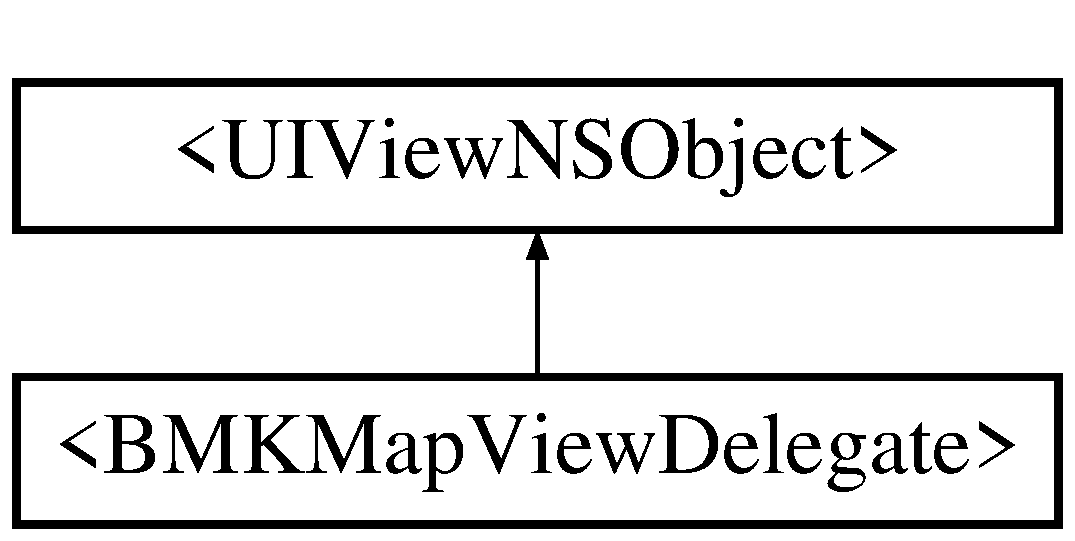
\includegraphics[height=2.000000cm]{protocol_b_m_k_map_view_delegate-p}
\end{center}
\end{figure}
\subsection*{实例方法}
\begin{DoxyCompactItemize}
\item 
(void) -\/ \hyperlink{protocol_b_m_k_map_view_delegate-p_ae87e30d1d70dd4e8dcff06b5e0cf51a7}{map\-View\-:region\-Will\-Change\-Animated\-:}
\item 
(void) -\/ \hyperlink{protocol_b_m_k_map_view_delegate-p_a6639906de681668b08204765528ce825}{map\-View\-:region\-Did\-Change\-Animated\-:}
\item 
(\hyperlink{interface_b_m_k_annotation_view}{B\-M\-K\-Annotation\-View} $\ast$) -\/ \hyperlink{protocol_b_m_k_map_view_delegate-p_a58eb111045e3e124bcf8abba4d1188d5}{map\-View\-:view\-For\-Annotation\-:}
\item 
(void) -\/ \hyperlink{protocol_b_m_k_map_view_delegate-p_ad982960181ac5b4087f4087e06f16603}{map\-View\-:did\-Add\-Annotation\-Views\-:}
\item 
(void) -\/ \hyperlink{protocol_b_m_k_map_view_delegate-p_a825411129229ae80dbd104596c0d788a}{map\-View\-:did\-Select\-Annotation\-View\-:}
\item 
(void) -\/ \hyperlink{protocol_b_m_k_map_view_delegate-p_a8b3c67fbfebc7d7479a1935269d8302d}{map\-View\-:did\-Deselect\-Annotation\-View\-:}
\item 
(void) -\/ \hyperlink{protocol_b_m_k_map_view_delegate-p_add2407adba384f1dd3c0953590e4a60d}{map\-View\-:annotation\-View\-:did\-Change\-Drag\-State\-:from\-Old\-State\-:}
\item 
(void) -\/ \hyperlink{protocol_b_m_k_map_view_delegate-p_adf11fcfbabf17146fd10d24f5b70aaf2}{map\-View\-:annotation\-View\-For\-Bubble\-:}
\item 
(\hyperlink{interface_b_m_k_overlay_view}{B\-M\-K\-Overlay\-View} $\ast$) -\/ \hyperlink{protocol_b_m_k_map_view_delegate-p_a643e260b01350f089451d745574e3d72}{map\-View\-:view\-For\-Overlay\-:}
\item 
(void) -\/ \hyperlink{protocol_b_m_k_map_view_delegate-p_a4eb0201fbe51ecd74d3b678a139435bf}{map\-View\-:did\-Add\-Overlay\-Views\-:}
\item 
(void) -\/ \hyperlink{protocol_b_m_k_map_view_delegate-p_ac3e98436fce2ee14c02837200e57a6fe}{map\-View\-:on\-Clicked\-Map\-Poi\-:}
\item 
(void) -\/ \hyperlink{protocol_b_m_k_map_view_delegate-p_a7e98b75f0edfc05ed93fda98f3fb682e}{map\-View\-:on\-Clicked\-Map\-Blank\-:}
\item 
(void) -\/ \hyperlink{protocol_b_m_k_map_view_delegate-p_a957fb04d2fb88bd0e45ad9d712c1e85f}{mapview\-:on\-Double\-Click\-:}
\item 
(void) -\/ \hyperlink{protocol_b_m_k_map_view_delegate-p_abdef3e78c6a4d51665bc859e16c629a4}{mapview\-:on\-Long\-Click\-:}
\item 
(void) -\/ \hyperlink{protocol_b_m_k_map_view_delegate-p_a2265718129af225330d0d5f350f45dd2}{map\-View\-Will\-Start\-Locating\-User\-:}
\item 
(void) -\/ \hyperlink{protocol_b_m_k_map_view_delegate-p_aac6507cc2dea1a2a7c2df80d08b42102}{map\-View\-Did\-Stop\-Locating\-User\-:}
\item 
(void) -\/ \hyperlink{protocol_b_m_k_map_view_delegate-p_a85fe7a69fc1924412e6a97d259157ab3}{map\-View\-:did\-Update\-User\-Location\-:}
\item 
(void) -\/ \hyperlink{protocol_b_m_k_map_view_delegate-p_a09254d3d99fa4c5777c646725b029966}{map\-View\-:did\-Fail\-To\-Locate\-User\-With\-Error\-:}
\end{DoxyCompactItemize}


\subsection{详细描述}
Map\-View的\-Delegate,map\-View通过此类来通知用户对应的事件 

\subsection{方法文档}
\hypertarget{protocol_b_m_k_map_view_delegate-p_add2407adba384f1dd3c0953590e4a60d}{\index{B\-M\-K\-Map\-View\-Delegate-\/p@{B\-M\-K\-Map\-View\-Delegate-\/p}!map\-View\-:annotation\-View\-:did\-Change\-Drag\-State\-:from\-Old\-State\-:@{map\-View\-:annotation\-View\-:did\-Change\-Drag\-State\-:from\-Old\-State\-:}}
\index{map\-View\-:annotation\-View\-:did\-Change\-Drag\-State\-:from\-Old\-State\-:@{map\-View\-:annotation\-View\-:did\-Change\-Drag\-State\-:from\-Old\-State\-:}!BMKMapViewDelegate-p@{B\-M\-K\-Map\-View\-Delegate-\/p}}
\subsubsection[{map\-View\-:annotation\-View\-:did\-Change\-Drag\-State\-:from\-Old\-State\-:}]{\setlength{\rightskip}{0pt plus 5cm}-\/ (void) map\-View\-: 
\begin{DoxyParamCaption}
\item[{({\bf B\-M\-K\-Map\-View} $\ast$)}]{map\-View}
\item[{annotationView:({\bf B\-M\-K\-Annotation\-View} $\ast$)}]{view}
\item[{didChangeDragState:(B\-M\-K\-Annotation\-View\-Drag\-State)}]{new\-State}
\item[{fromOldState:(B\-M\-K\-Annotation\-View\-Drag\-State)}]{old\-State}
\end{DoxyParamCaption}
\hspace{0.3cm}{\ttfamily [optional]}}}\label{protocol_b_m_k_map_view_delegate-p_add2407adba384f1dd3c0953590e4a60d}
拖动annotation view时,若view的状态发生变化,会调用此函数。ios3.2以后支持 
\begin{DoxyParams}{参数}
{\em map\-View} & 地图\-View \\
\hline
{\em view} & annotation view \\
\hline
{\em new\-State} & 新状态 \\
\hline
{\em old\-State} & 旧状态 \\
\hline
\end{DoxyParams}
\hypertarget{protocol_b_m_k_map_view_delegate-p_adf11fcfbabf17146fd10d24f5b70aaf2}{\index{B\-M\-K\-Map\-View\-Delegate-\/p@{B\-M\-K\-Map\-View\-Delegate-\/p}!map\-View\-:annotation\-View\-For\-Bubble\-:@{map\-View\-:annotation\-View\-For\-Bubble\-:}}
\index{map\-View\-:annotation\-View\-For\-Bubble\-:@{map\-View\-:annotation\-View\-For\-Bubble\-:}!BMKMapViewDelegate-p@{B\-M\-K\-Map\-View\-Delegate-\/p}}
\subsubsection[{map\-View\-:annotation\-View\-For\-Bubble\-:}]{\setlength{\rightskip}{0pt plus 5cm}-\/ (void) map\-View\-: 
\begin{DoxyParamCaption}
\item[{({\bf B\-M\-K\-Map\-View} $\ast$)}]{map\-View}
\item[{annotationViewForBubble:({\bf B\-M\-K\-Annotation\-View} $\ast$)}]{view}
\end{DoxyParamCaption}
\hspace{0.3cm}{\ttfamily [optional]}}}\label{protocol_b_m_k_map_view_delegate-p_adf11fcfbabf17146fd10d24f5b70aaf2}
当点击annotation view弹出的泡泡时,调用此接口 
\begin{DoxyParams}{参数}
{\em map\-View} & 地图\-View \\
\hline
{\em view} & 泡泡所属的annotation view \\
\hline
\end{DoxyParams}
\hypertarget{protocol_b_m_k_map_view_delegate-p_ad982960181ac5b4087f4087e06f16603}{\index{B\-M\-K\-Map\-View\-Delegate-\/p@{B\-M\-K\-Map\-View\-Delegate-\/p}!map\-View\-:did\-Add\-Annotation\-Views\-:@{map\-View\-:did\-Add\-Annotation\-Views\-:}}
\index{map\-View\-:did\-Add\-Annotation\-Views\-:@{map\-View\-:did\-Add\-Annotation\-Views\-:}!BMKMapViewDelegate-p@{B\-M\-K\-Map\-View\-Delegate-\/p}}
\subsubsection[{map\-View\-:did\-Add\-Annotation\-Views\-:}]{\setlength{\rightskip}{0pt plus 5cm}-\/ (void) map\-View\-: 
\begin{DoxyParamCaption}
\item[{({\bf B\-M\-K\-Map\-View} $\ast$)}]{map\-View}
\item[{didAddAnnotationViews:(N\-S\-Array $\ast$)}]{views}
\end{DoxyParamCaption}
\hspace{0.3cm}{\ttfamily [optional]}}}\label{protocol_b_m_k_map_view_delegate-p_ad982960181ac5b4087f4087e06f16603}
当map\-View新添加annotation views时,调用此接口 
\begin{DoxyParams}{参数}
{\em map\-View} & 地图\-View \\
\hline
{\em views} & 新添加的annotation views \\
\hline
\end{DoxyParams}
\hypertarget{protocol_b_m_k_map_view_delegate-p_a4eb0201fbe51ecd74d3b678a139435bf}{\index{B\-M\-K\-Map\-View\-Delegate-\/p@{B\-M\-K\-Map\-View\-Delegate-\/p}!map\-View\-:did\-Add\-Overlay\-Views\-:@{map\-View\-:did\-Add\-Overlay\-Views\-:}}
\index{map\-View\-:did\-Add\-Overlay\-Views\-:@{map\-View\-:did\-Add\-Overlay\-Views\-:}!BMKMapViewDelegate-p@{B\-M\-K\-Map\-View\-Delegate-\/p}}
\subsubsection[{map\-View\-:did\-Add\-Overlay\-Views\-:}]{\setlength{\rightskip}{0pt plus 5cm}-\/ (void) map\-View\-: 
\begin{DoxyParamCaption}
\item[{({\bf B\-M\-K\-Map\-View} $\ast$)}]{map\-View}
\item[{didAddOverlayViews:(N\-S\-Array $\ast$)}]{overlay\-Views}
\end{DoxyParamCaption}
\hspace{0.3cm}{\ttfamily [optional]}}}\label{protocol_b_m_k_map_view_delegate-p_a4eb0201fbe51ecd74d3b678a139435bf}
当map\-View新添加overlay views时,调用此接口 
\begin{DoxyParams}{参数}
{\em map\-View} & 地图\-View \\
\hline
{\em overlay\-Views} & 新添加的overlay views \\
\hline
\end{DoxyParams}
\hypertarget{protocol_b_m_k_map_view_delegate-p_a8b3c67fbfebc7d7479a1935269d8302d}{\index{B\-M\-K\-Map\-View\-Delegate-\/p@{B\-M\-K\-Map\-View\-Delegate-\/p}!map\-View\-:did\-Deselect\-Annotation\-View\-:@{map\-View\-:did\-Deselect\-Annotation\-View\-:}}
\index{map\-View\-:did\-Deselect\-Annotation\-View\-:@{map\-View\-:did\-Deselect\-Annotation\-View\-:}!BMKMapViewDelegate-p@{B\-M\-K\-Map\-View\-Delegate-\/p}}
\subsubsection[{map\-View\-:did\-Deselect\-Annotation\-View\-:}]{\setlength{\rightskip}{0pt plus 5cm}-\/ (void) map\-View\-: 
\begin{DoxyParamCaption}
\item[{({\bf B\-M\-K\-Map\-View} $\ast$)}]{map\-View}
\item[{didDeselectAnnotationView:({\bf B\-M\-K\-Annotation\-View} $\ast$)}]{view}
\end{DoxyParamCaption}
\hspace{0.3cm}{\ttfamily [optional]}}}\label{protocol_b_m_k_map_view_delegate-p_a8b3c67fbfebc7d7479a1935269d8302d}
当取消选中一个annotation views时,调用此接口 
\begin{DoxyParams}{参数}
{\em map\-View} & 地图\-View \\
\hline
{\em views} & 取消选中的annotation views \\
\hline
\end{DoxyParams}
\hypertarget{protocol_b_m_k_map_view_delegate-p_a09254d3d99fa4c5777c646725b029966}{\index{B\-M\-K\-Map\-View\-Delegate-\/p@{B\-M\-K\-Map\-View\-Delegate-\/p}!map\-View\-:did\-Fail\-To\-Locate\-User\-With\-Error\-:@{map\-View\-:did\-Fail\-To\-Locate\-User\-With\-Error\-:}}
\index{map\-View\-:did\-Fail\-To\-Locate\-User\-With\-Error\-:@{map\-View\-:did\-Fail\-To\-Locate\-User\-With\-Error\-:}!BMKMapViewDelegate-p@{B\-M\-K\-Map\-View\-Delegate-\/p}}
\subsubsection[{map\-View\-:did\-Fail\-To\-Locate\-User\-With\-Error\-:}]{\setlength{\rightskip}{0pt plus 5cm}-\/ (void) map\-View\-: 
\begin{DoxyParamCaption}
\item[{({\bf B\-M\-K\-Map\-View} $\ast$)}]{map\-View}
\item[{didFailToLocateUserWithError:(N\-S\-Error $\ast$)}]{error}
\end{DoxyParamCaption}
\hspace{0.3cm}{\ttfamily [optional]}}}\label{protocol_b_m_k_map_view_delegate-p_a09254d3d99fa4c5777c646725b029966}
定位失败后,会调用此函数 
\begin{DoxyParams}{参数}
{\em map\-View} & 地图\-View \\
\hline
{\em error} & 错误号,参考\-C\-L\-Error.\-h中定义的错误号 \\
\hline
\end{DoxyParams}
\hypertarget{protocol_b_m_k_map_view_delegate-p_a825411129229ae80dbd104596c0d788a}{\index{B\-M\-K\-Map\-View\-Delegate-\/p@{B\-M\-K\-Map\-View\-Delegate-\/p}!map\-View\-:did\-Select\-Annotation\-View\-:@{map\-View\-:did\-Select\-Annotation\-View\-:}}
\index{map\-View\-:did\-Select\-Annotation\-View\-:@{map\-View\-:did\-Select\-Annotation\-View\-:}!BMKMapViewDelegate-p@{B\-M\-K\-Map\-View\-Delegate-\/p}}
\subsubsection[{map\-View\-:did\-Select\-Annotation\-View\-:}]{\setlength{\rightskip}{0pt plus 5cm}-\/ (void) map\-View\-: 
\begin{DoxyParamCaption}
\item[{({\bf B\-M\-K\-Map\-View} $\ast$)}]{map\-View}
\item[{didSelectAnnotationView:({\bf B\-M\-K\-Annotation\-View} $\ast$)}]{view}
\end{DoxyParamCaption}
\hspace{0.3cm}{\ttfamily [optional]}}}\label{protocol_b_m_k_map_view_delegate-p_a825411129229ae80dbd104596c0d788a}
当选中一个annotation views时,调用此接口 
\begin{DoxyParams}{参数}
{\em map\-View} & 地图\-View \\
\hline
{\em views} & 选中的annotation views \\
\hline
\end{DoxyParams}
\hypertarget{protocol_b_m_k_map_view_delegate-p_a85fe7a69fc1924412e6a97d259157ab3}{\index{B\-M\-K\-Map\-View\-Delegate-\/p@{B\-M\-K\-Map\-View\-Delegate-\/p}!map\-View\-:did\-Update\-User\-Location\-:@{map\-View\-:did\-Update\-User\-Location\-:}}
\index{map\-View\-:did\-Update\-User\-Location\-:@{map\-View\-:did\-Update\-User\-Location\-:}!BMKMapViewDelegate-p@{B\-M\-K\-Map\-View\-Delegate-\/p}}
\subsubsection[{map\-View\-:did\-Update\-User\-Location\-:}]{\setlength{\rightskip}{0pt plus 5cm}-\/ (void) map\-View\-: 
\begin{DoxyParamCaption}
\item[{({\bf B\-M\-K\-Map\-View} $\ast$)}]{map\-View}
\item[{didUpdateUserLocation:({\bf B\-M\-K\-User\-Location} $\ast$)}]{user\-Location}
\end{DoxyParamCaption}
\hspace{0.3cm}{\ttfamily [optional]}}}\label{protocol_b_m_k_map_view_delegate-p_a85fe7a69fc1924412e6a97d259157ab3}
用户位置更新后,会调用此函数 
\begin{DoxyParams}{参数}
{\em map\-View} & 地图\-View \\
\hline
{\em user\-Location} & 新的用户位置 \\
\hline
\end{DoxyParams}
\hypertarget{protocol_b_m_k_map_view_delegate-p_a7e98b75f0edfc05ed93fda98f3fb682e}{\index{B\-M\-K\-Map\-View\-Delegate-\/p@{B\-M\-K\-Map\-View\-Delegate-\/p}!map\-View\-:on\-Clicked\-Map\-Blank\-:@{map\-View\-:on\-Clicked\-Map\-Blank\-:}}
\index{map\-View\-:on\-Clicked\-Map\-Blank\-:@{map\-View\-:on\-Clicked\-Map\-Blank\-:}!BMKMapViewDelegate-p@{B\-M\-K\-Map\-View\-Delegate-\/p}}
\subsubsection[{map\-View\-:on\-Clicked\-Map\-Blank\-:}]{\setlength{\rightskip}{0pt plus 5cm}-\/ (void) map\-View\-: 
\begin{DoxyParamCaption}
\item[{({\bf B\-M\-K\-Map\-View} $\ast$)}]{map\-View}
\item[{onClickedMapBlank:(C\-L\-Location\-Coordinate2\-D)}]{coordinate}
\end{DoxyParamCaption}
\hspace{0.3cm}{\ttfamily [optional]}}}\label{protocol_b_m_k_map_view_delegate-p_a7e98b75f0edfc05ed93fda98f3fb682e}
点中底图空白处会回调此接口 
\begin{DoxyParams}{参数}
{\em mapview} & 地图\-View \\
\hline
{\em coordinate} & 空白处坐标点的经纬度 \\
\hline
\end{DoxyParams}
\hypertarget{protocol_b_m_k_map_view_delegate-p_ac3e98436fce2ee14c02837200e57a6fe}{\index{B\-M\-K\-Map\-View\-Delegate-\/p@{B\-M\-K\-Map\-View\-Delegate-\/p}!map\-View\-:on\-Clicked\-Map\-Poi\-:@{map\-View\-:on\-Clicked\-Map\-Poi\-:}}
\index{map\-View\-:on\-Clicked\-Map\-Poi\-:@{map\-View\-:on\-Clicked\-Map\-Poi\-:}!BMKMapViewDelegate-p@{B\-M\-K\-Map\-View\-Delegate-\/p}}
\subsubsection[{map\-View\-:on\-Clicked\-Map\-Poi\-:}]{\setlength{\rightskip}{0pt plus 5cm}-\/ (void) map\-View\-: 
\begin{DoxyParamCaption}
\item[{({\bf B\-M\-K\-Map\-View} $\ast$)}]{map\-View}
\item[{onClickedMapPoi:({\bf B\-M\-K\-Map\-Poi} $\ast$)}]{map\-Poi}
\end{DoxyParamCaption}
\hspace{0.3cm}{\ttfamily [optional]}}}\label{protocol_b_m_k_map_view_delegate-p_ac3e98436fce2ee14c02837200e57a6fe}
点中底图标注后会回调此接口 
\begin{DoxyParams}{参数}
{\em mapview} & 地图\-View \\
\hline
{\em map\-Poi} & 标注点信息 \\
\hline
\end{DoxyParams}
\hypertarget{protocol_b_m_k_map_view_delegate-p_a957fb04d2fb88bd0e45ad9d712c1e85f}{\index{B\-M\-K\-Map\-View\-Delegate-\/p@{B\-M\-K\-Map\-View\-Delegate-\/p}!mapview\-:on\-Double\-Click\-:@{mapview\-:on\-Double\-Click\-:}}
\index{mapview\-:on\-Double\-Click\-:@{mapview\-:on\-Double\-Click\-:}!BMKMapViewDelegate-p@{B\-M\-K\-Map\-View\-Delegate-\/p}}
\subsubsection[{mapview\-:on\-Double\-Click\-:}]{\setlength{\rightskip}{0pt plus 5cm}-\/ (void) mapview\-: 
\begin{DoxyParamCaption}
\item[{({\bf B\-M\-K\-Map\-View} $\ast$)}]{map\-View}
\item[{onDoubleClick:(C\-L\-Location\-Coordinate2\-D)}]{coordinate}
\end{DoxyParamCaption}
\hspace{0.3cm}{\ttfamily [optional]}}}\label{protocol_b_m_k_map_view_delegate-p_a957fb04d2fb88bd0e45ad9d712c1e85f}
双击地图时会回调此接口 
\begin{DoxyParams}{参数}
{\em mapview} & 地图\-View \\
\hline
{\em coordinate} & 返回双击处坐标点的经纬度 \\
\hline
\end{DoxyParams}
\hypertarget{protocol_b_m_k_map_view_delegate-p_abdef3e78c6a4d51665bc859e16c629a4}{\index{B\-M\-K\-Map\-View\-Delegate-\/p@{B\-M\-K\-Map\-View\-Delegate-\/p}!mapview\-:on\-Long\-Click\-:@{mapview\-:on\-Long\-Click\-:}}
\index{mapview\-:on\-Long\-Click\-:@{mapview\-:on\-Long\-Click\-:}!BMKMapViewDelegate-p@{B\-M\-K\-Map\-View\-Delegate-\/p}}
\subsubsection[{mapview\-:on\-Long\-Click\-:}]{\setlength{\rightskip}{0pt plus 5cm}-\/ (void) mapview\-: 
\begin{DoxyParamCaption}
\item[{({\bf B\-M\-K\-Map\-View} $\ast$)}]{map\-View}
\item[{onLongClick:(C\-L\-Location\-Coordinate2\-D)}]{coordinate}
\end{DoxyParamCaption}
\hspace{0.3cm}{\ttfamily [optional]}}}\label{protocol_b_m_k_map_view_delegate-p_abdef3e78c6a4d51665bc859e16c629a4}
长按地图时会回调此接口 
\begin{DoxyParams}{参数}
{\em mapview} & 地图\-View \\
\hline
{\em coordinate} & 返回长按事件坐标点的经纬度 \\
\hline
\end{DoxyParams}
\hypertarget{protocol_b_m_k_map_view_delegate-p_a6639906de681668b08204765528ce825}{\index{B\-M\-K\-Map\-View\-Delegate-\/p@{B\-M\-K\-Map\-View\-Delegate-\/p}!map\-View\-:region\-Did\-Change\-Animated\-:@{map\-View\-:region\-Did\-Change\-Animated\-:}}
\index{map\-View\-:region\-Did\-Change\-Animated\-:@{map\-View\-:region\-Did\-Change\-Animated\-:}!BMKMapViewDelegate-p@{B\-M\-K\-Map\-View\-Delegate-\/p}}
\subsubsection[{map\-View\-:region\-Did\-Change\-Animated\-:}]{\setlength{\rightskip}{0pt plus 5cm}-\/ (void) map\-View\-: 
\begin{DoxyParamCaption}
\item[{({\bf B\-M\-K\-Map\-View} $\ast$)}]{map\-View}
\item[{regionDidChangeAnimated:(B\-O\-O\-L)}]{animated}
\end{DoxyParamCaption}
\hspace{0.3cm}{\ttfamily [optional]}}}\label{protocol_b_m_k_map_view_delegate-p_a6639906de681668b08204765528ce825}
地图区域改变完成后会调用此接口 
\begin{DoxyParams}{参数}
{\em mapview} & 地图\-View \\
\hline
{\em animated} & 是否动画 \\
\hline
\end{DoxyParams}
\hypertarget{protocol_b_m_k_map_view_delegate-p_ae87e30d1d70dd4e8dcff06b5e0cf51a7}{\index{B\-M\-K\-Map\-View\-Delegate-\/p@{B\-M\-K\-Map\-View\-Delegate-\/p}!map\-View\-:region\-Will\-Change\-Animated\-:@{map\-View\-:region\-Will\-Change\-Animated\-:}}
\index{map\-View\-:region\-Will\-Change\-Animated\-:@{map\-View\-:region\-Will\-Change\-Animated\-:}!BMKMapViewDelegate-p@{B\-M\-K\-Map\-View\-Delegate-\/p}}
\subsubsection[{map\-View\-:region\-Will\-Change\-Animated\-:}]{\setlength{\rightskip}{0pt plus 5cm}-\/ (void) map\-View\-: 
\begin{DoxyParamCaption}
\item[{({\bf B\-M\-K\-Map\-View} $\ast$)}]{map\-View}
\item[{regionWillChangeAnimated:(B\-O\-O\-L)}]{animated}
\end{DoxyParamCaption}
\hspace{0.3cm}{\ttfamily [optional]}}}\label{protocol_b_m_k_map_view_delegate-p_ae87e30d1d70dd4e8dcff06b5e0cf51a7}
地图区域即将改变时会调用此接口 
\begin{DoxyParams}{参数}
{\em mapview} & 地图\-View \\
\hline
{\em animated} & 是否动画 \\
\hline
\end{DoxyParams}
\hypertarget{protocol_b_m_k_map_view_delegate-p_a58eb111045e3e124bcf8abba4d1188d5}{\index{B\-M\-K\-Map\-View\-Delegate-\/p@{B\-M\-K\-Map\-View\-Delegate-\/p}!map\-View\-:view\-For\-Annotation\-:@{map\-View\-:view\-For\-Annotation\-:}}
\index{map\-View\-:view\-For\-Annotation\-:@{map\-View\-:view\-For\-Annotation\-:}!BMKMapViewDelegate-p@{B\-M\-K\-Map\-View\-Delegate-\/p}}
\subsubsection[{map\-View\-:view\-For\-Annotation\-:}]{\setlength{\rightskip}{0pt plus 5cm}-\/ ({\bf B\-M\-K\-Annotation\-View} $\ast$) map\-View\-: 
\begin{DoxyParamCaption}
\item[{({\bf B\-M\-K\-Map\-View} $\ast$)}]{map\-View}
\item[{viewForAnnotation:(id$<$ {\bf B\-M\-K\-Annotation} $>$)}]{annotation}
\end{DoxyParamCaption}
\hspace{0.3cm}{\ttfamily [optional]}}}\label{protocol_b_m_k_map_view_delegate-p_a58eb111045e3e124bcf8abba4d1188d5}
根据anntation生成对应的\-View 
\begin{DoxyParams}{参数}
{\em map\-View} & 地图\-View \\
\hline
{\em annotation} & 指定的标注 \\
\hline
\end{DoxyParams}
\begin{DoxyReturn}{返回}
生成的标注\-View 
\end{DoxyReturn}
\hypertarget{protocol_b_m_k_map_view_delegate-p_a643e260b01350f089451d745574e3d72}{\index{B\-M\-K\-Map\-View\-Delegate-\/p@{B\-M\-K\-Map\-View\-Delegate-\/p}!map\-View\-:view\-For\-Overlay\-:@{map\-View\-:view\-For\-Overlay\-:}}
\index{map\-View\-:view\-For\-Overlay\-:@{map\-View\-:view\-For\-Overlay\-:}!BMKMapViewDelegate-p@{B\-M\-K\-Map\-View\-Delegate-\/p}}
\subsubsection[{map\-View\-:view\-For\-Overlay\-:}]{\setlength{\rightskip}{0pt plus 5cm}-\/ ({\bf B\-M\-K\-Overlay\-View} $\ast$) map\-View\-: 
\begin{DoxyParamCaption}
\item[{({\bf B\-M\-K\-Map\-View} $\ast$)}]{map\-View}
\item[{viewForOverlay:(id$<$ {\bf B\-M\-K\-Overlay} $>$)}]{overlay}
\end{DoxyParamCaption}
\hspace{0.3cm}{\ttfamily [optional]}}}\label{protocol_b_m_k_map_view_delegate-p_a643e260b01350f089451d745574e3d72}
根据overlay生成对应的\-View 
\begin{DoxyParams}{参数}
{\em map\-View} & 地图\-View \\
\hline
{\em overlay} & 指定的overlay \\
\hline
\end{DoxyParams}
\begin{DoxyReturn}{返回}
生成的覆盖物\-View 
\end{DoxyReturn}
\hypertarget{protocol_b_m_k_map_view_delegate-p_aac6507cc2dea1a2a7c2df80d08b42102}{\index{B\-M\-K\-Map\-View\-Delegate-\/p@{B\-M\-K\-Map\-View\-Delegate-\/p}!map\-View\-Did\-Stop\-Locating\-User\-:@{map\-View\-Did\-Stop\-Locating\-User\-:}}
\index{map\-View\-Did\-Stop\-Locating\-User\-:@{map\-View\-Did\-Stop\-Locating\-User\-:}!BMKMapViewDelegate-p@{B\-M\-K\-Map\-View\-Delegate-\/p}}
\subsubsection[{map\-View\-Did\-Stop\-Locating\-User\-:}]{\setlength{\rightskip}{0pt plus 5cm}-\/ (void) map\-View\-Did\-Stop\-Locating\-User\-: 
\begin{DoxyParamCaption}
\item[{({\bf B\-M\-K\-Map\-View} $\ast$)}]{map\-View}
\end{DoxyParamCaption}
\hspace{0.3cm}{\ttfamily [optional]}}}\label{protocol_b_m_k_map_view_delegate-p_aac6507cc2dea1a2a7c2df80d08b42102}
在地图\-View停止定位后,会调用此函数 
\begin{DoxyParams}{参数}
{\em map\-View} & 地图\-View \\
\hline
\end{DoxyParams}
\hypertarget{protocol_b_m_k_map_view_delegate-p_a2265718129af225330d0d5f350f45dd2}{\index{B\-M\-K\-Map\-View\-Delegate-\/p@{B\-M\-K\-Map\-View\-Delegate-\/p}!map\-View\-Will\-Start\-Locating\-User\-:@{map\-View\-Will\-Start\-Locating\-User\-:}}
\index{map\-View\-Will\-Start\-Locating\-User\-:@{map\-View\-Will\-Start\-Locating\-User\-:}!BMKMapViewDelegate-p@{B\-M\-K\-Map\-View\-Delegate-\/p}}
\subsubsection[{map\-View\-Will\-Start\-Locating\-User\-:}]{\setlength{\rightskip}{0pt plus 5cm}-\/ (void) map\-View\-Will\-Start\-Locating\-User\-: 
\begin{DoxyParamCaption}
\item[{({\bf B\-M\-K\-Map\-View} $\ast$)}]{map\-View}
\end{DoxyParamCaption}
\hspace{0.3cm}{\ttfamily [optional]}}}\label{protocol_b_m_k_map_view_delegate-p_a2265718129af225330d0d5f350f45dd2}
在地图\-View将要启动定位时,会调用此函数 
\begin{DoxyParams}{参数}
{\em map\-View} & 地图\-View \\
\hline
\end{DoxyParams}


The documentation for this protocol was generated from the following file\-:\begin{DoxyCompactItemize}
\item 
B\-M\-K\-Map\-View.\-h\end{DoxyCompactItemize}

\hypertarget{interface_b_m_k_multi_point}{\section{B\-M\-K\-Multi\-Point 类参考}
\label{interface_b_m_k_multi_point}\index{B\-M\-K\-Multi\-Point@{B\-M\-K\-Multi\-Point}}
}


该类定义多个点,是个由多个点组成的虚基类, 不能直接实例化对象, 要使用其子类\-B\-M\-K\-Polyline,B\-M\-K\-Polygon来实例化  




{\ttfamily \#import $<$B\-M\-K\-Multi\-Point.\-h$>$}

继承关系图 B\-M\-K\-Multi\-Point\-:\begin{figure}[H]
\begin{center}
\leavevmode
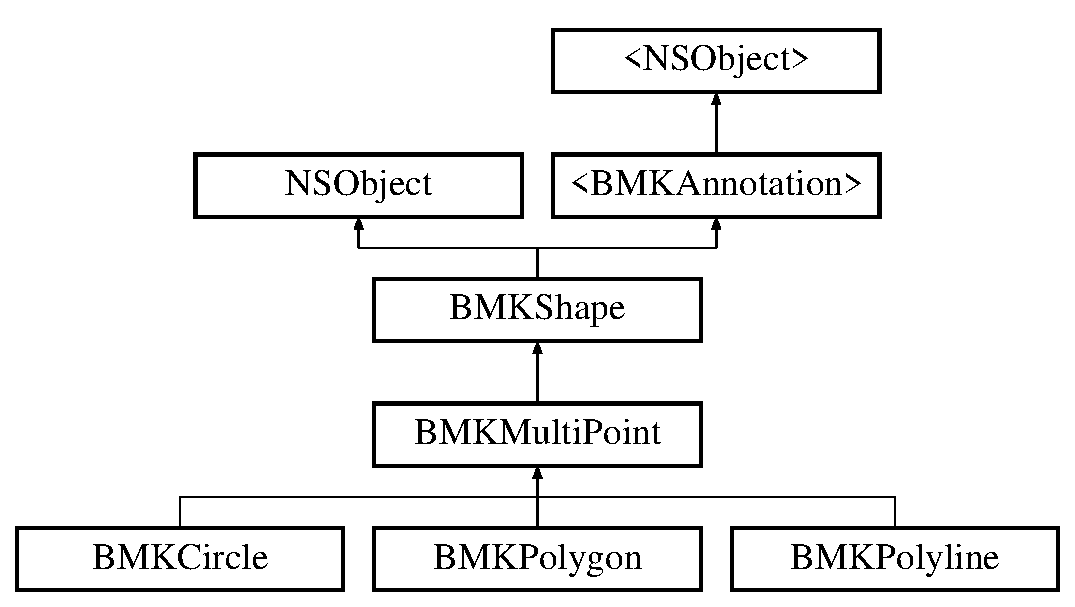
\includegraphics[height=5.000000cm]{interface_b_m_k_multi_point}
\end{center}
\end{figure}
\subsection*{实例方法}
\begin{DoxyCompactItemize}
\item 
(void) -\/ \hyperlink{interface_b_m_k_multi_point_a5d7b000029db5c7efb2230ccb980bc29}{get\-Coordinates\-:range\-:}
\end{DoxyCompactItemize}
\subsection*{保护成员变量}
\begin{DoxyCompactItemize}
\item 
\hypertarget{interface_b_m_k_multi_point_a736d72334fd2ca7ae2108d9692d1107c}{package \hyperlink{struct_b_m_k_map_point}{B\-M\-K\-Map\-Point} $\ast$ {\bfseries \-\_\-points}}\label{interface_b_m_k_multi_point_a736d72334fd2ca7ae2108d9692d1107c}

\item 
\hypertarget{interface_b_m_k_multi_point_a8cc584110411ad5f72fc5068ae123a32}{N\-S\-U\-Integer {\bfseries \-\_\-point\-Count}}\label{interface_b_m_k_multi_point_a8cc584110411ad5f72fc5068ae123a32}

\item 
\hypertarget{interface_b_m_k_multi_point_a25b2435a2c10b3a22f6e7dc5bd064a52}{\hyperlink{struct_b_m_k_map_rect}{B\-M\-K\-Map\-Rect} {\bfseries \-\_\-bounding\-Rect}}\label{interface_b_m_k_multi_point_a25b2435a2c10b3a22f6e7dc5bd064a52}

\end{DoxyCompactItemize}
\subsection*{Properties}
\begin{DoxyCompactItemize}
\item 
\hypertarget{interface_b_m_k_multi_point_aa810056a59644284eb13fca968124e0c}{\hyperlink{struct_b_m_k_map_point}{B\-M\-K\-Map\-Point} $\ast$ \hyperlink{interface_b_m_k_multi_point_aa810056a59644284eb13fca968124e0c}{points}}\label{interface_b_m_k_multi_point_aa810056a59644284eb13fca968124e0c}

\begin{DoxyCompactList}\small\item\em 坐标点数组 \end{DoxyCompactList}\item 
\hypertarget{interface_b_m_k_multi_point_a717b76bf8c1c25ce7ae11c959fb4af9f}{N\-S\-U\-Integer \hyperlink{interface_b_m_k_multi_point_a717b76bf8c1c25ce7ae11c959fb4af9f}{point\-Count}}\label{interface_b_m_k_multi_point_a717b76bf8c1c25ce7ae11c959fb4af9f}

\begin{DoxyCompactList}\small\item\em 坐标点的个数 \end{DoxyCompactList}\end{DoxyCompactItemize}


\subsection{详细描述}
该类定义多个点,是个由多个点组成的虚基类, 不能直接实例化对象, 要使用其子类\-B\-M\-K\-Polyline,B\-M\-K\-Polygon来实例化 

\subsection{方法文档}
\hypertarget{interface_b_m_k_multi_point_a5d7b000029db5c7efb2230ccb980bc29}{\index{B\-M\-K\-Multi\-Point@{B\-M\-K\-Multi\-Point}!get\-Coordinates\-:range\-:@{get\-Coordinates\-:range\-:}}
\index{get\-Coordinates\-:range\-:@{get\-Coordinates\-:range\-:}!BMKMultiPoint@{B\-M\-K\-Multi\-Point}}
\subsubsection[{get\-Coordinates\-:range\-:}]{\setlength{\rightskip}{0pt plus 5cm}-\/ (void) get\-Coordinates\-: 
\begin{DoxyParamCaption}
\item[{(C\-L\-Location\-Coordinate2\-D $\ast$)}]{coords}
\item[{range:(N\-S\-Range)}]{range}
\end{DoxyParamCaption}
}}\label{interface_b_m_k_multi_point_a5d7b000029db5c7efb2230ccb980bc29}
将内部的直角坐标数据转换为经纬度坐标点数据,并拷贝到指定的数组中 
\begin{DoxyParams}{参数}
{\em coords} & 经纬度坐标数组,转换后的坐标将存储到该数组中,该数组长度必须大于等于要拷贝的坐标点的个数(range.\-length) \\
\hline
{\em range} & 指定要拷贝的数据段 \\
\hline
\end{DoxyParams}


The documentation for this class was generated from the following file\-:\begin{DoxyCompactItemize}
\item 
B\-M\-K\-Multi\-Point.\-h\end{DoxyCompactItemize}

\hypertarget{interface_b_m_k_offline_map}{\section{B\-M\-K\-Offline\-Map 类参考}
\label{interface_b_m_k_offline_map}\index{B\-M\-K\-Offline\-Map@{B\-M\-K\-Offline\-Map}}
}


离线地图服务  




{\ttfamily \#import $<$B\-M\-K\-Offline\-Map.\-h$>$}

继承关系图 B\-M\-K\-Offline\-Map\-:\begin{figure}[H]
\begin{center}
\leavevmode
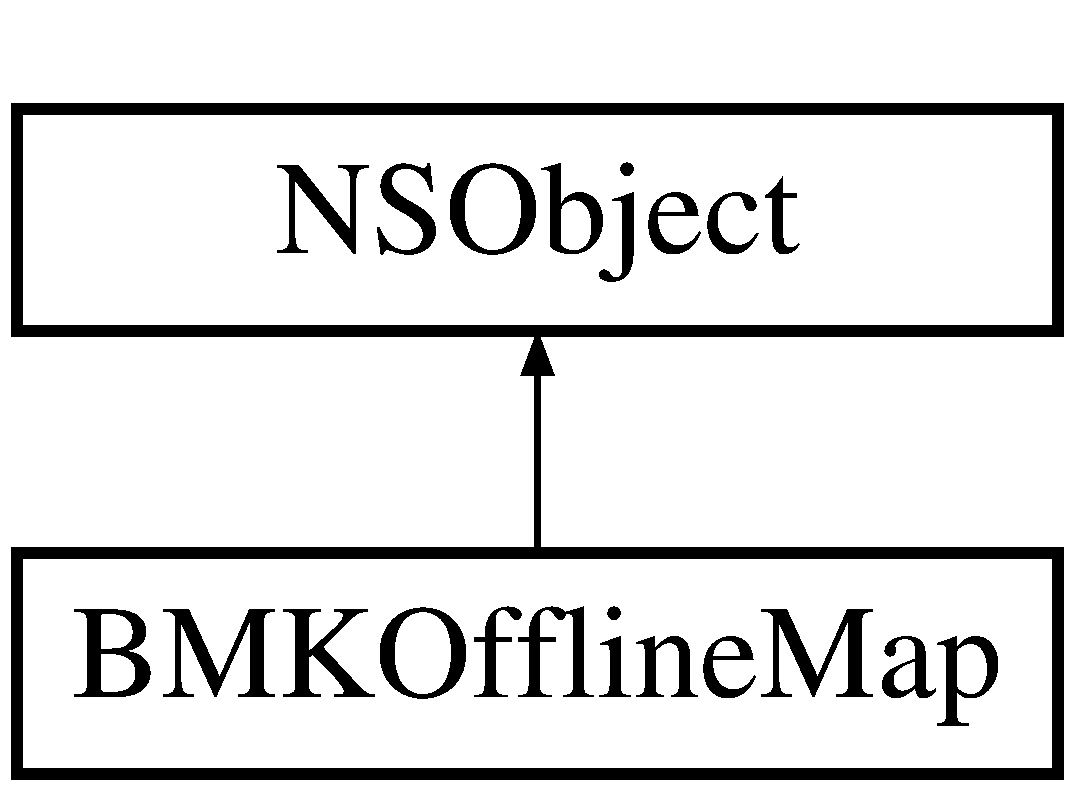
\includegraphics[height=2.000000cm]{interface_b_m_k_offline_map}
\end{center}
\end{figure}
\subsection*{实例方法}
\begin{DoxyCompactItemize}
\item 
(B\-O\-O\-L) -\/ \hyperlink{interface_b_m_k_offline_map_a2074d1fd832b6e5c84ab6b1c438a3b1f}{scan\-:}
\item 
(B\-O\-O\-L) -\/ \hyperlink{interface_b_m_k_offline_map_a40aa794e96677e472bf0d6f2ac18d583}{start\-:}
\item 
(B\-O\-O\-L) -\/ \hyperlink{interface_b_m_k_offline_map_a4c2489e1502d34bd807a1c4418560f88}{update\-:}
\item 
(B\-O\-O\-L) -\/ \hyperlink{interface_b_m_k_offline_map_a9c601d81b148c729342863db92b47831}{pause\-:}
\item 
(B\-O\-O\-L) -\/ \hyperlink{interface_b_m_k_offline_map_ac834ae7e577d2fa4dc864232b30f02df}{remove\-:}
\item 
(N\-S\-Array $\ast$) -\/ \hyperlink{interface_b_m_k_offline_map_a35c1c36472716ec22cacd54c5c710a5e}{get\-Hot\-City\-List}
\item 
(N\-S\-Array $\ast$) -\/ \hyperlink{interface_b_m_k_offline_map_a9a78b1a176ea59abe1b26e237a6e3a2c}{get\-Offline\-City\-List}
\item 
(N\-S\-Array $\ast$) -\/ \hyperlink{interface_b_m_k_offline_map_a9447d5aed62366152b3b6978b9fc1d34}{search\-City\-:}
\item 
(N\-S\-Array $\ast$) -\/ \hyperlink{interface_b_m_k_offline_map_a3152e5d5076958cda782d20565ceea56}{get\-All\-Update\-Info}
\item 
(\hyperlink{interface_b_m_k_o_l_update_element}{B\-M\-K\-O\-L\-Update\-Element} $\ast$) -\/ \hyperlink{interface_b_m_k_offline_map_ab11a98584ffd1f5582a2439a794646cb}{get\-Update\-Info\-:}
\end{DoxyCompactItemize}
\subsection*{Properties}
\begin{DoxyCompactItemize}
\item 
\hypertarget{interface_b_m_k_offline_map_ae25b1af7e710b8dbffd88aad3e081f48}{id$<$ \hyperlink{protocol_b_m_k_offline_map_delegate-p}{B\-M\-K\-Offline\-Map\-Delegate} $>$ {\bfseries delegate}}\label{interface_b_m_k_offline_map_ae25b1af7e710b8dbffd88aad3e081f48}

\end{DoxyCompactItemize}


\subsection{详细描述}
离线地图服务 

\subsection{方法文档}
\hypertarget{interface_b_m_k_offline_map_a3152e5d5076958cda782d20565ceea56}{\index{B\-M\-K\-Offline\-Map@{B\-M\-K\-Offline\-Map}!get\-All\-Update\-Info@{get\-All\-Update\-Info}}
\index{get\-All\-Update\-Info@{get\-All\-Update\-Info}!BMKOfflineMap@{B\-M\-K\-Offline\-Map}}
\subsubsection[{get\-All\-Update\-Info}]{\setlength{\rightskip}{0pt plus 5cm}-\/ (N\-S\-Array$\ast$) get\-All\-Update\-Info 
\begin{DoxyParamCaption}
{}
\end{DoxyParamCaption}
}}\label{interface_b_m_k_offline_map_a3152e5d5076958cda782d20565ceea56}
返回各城市离线地图更新信息 \begin{DoxyReturn}{返回}
各城市离线地图更新信息,用户需要显示释放该数组,数组元素为\-B\-M\-K\-O\-L\-Update\-Element 
\end{DoxyReturn}
\hypertarget{interface_b_m_k_offline_map_a35c1c36472716ec22cacd54c5c710a5e}{\index{B\-M\-K\-Offline\-Map@{B\-M\-K\-Offline\-Map}!get\-Hot\-City\-List@{get\-Hot\-City\-List}}
\index{get\-Hot\-City\-List@{get\-Hot\-City\-List}!BMKOfflineMap@{B\-M\-K\-Offline\-Map}}
\subsubsection[{get\-Hot\-City\-List}]{\setlength{\rightskip}{0pt plus 5cm}-\/ (N\-S\-Array$\ast$) get\-Hot\-City\-List 
\begin{DoxyParamCaption}
{}
\end{DoxyParamCaption}
}}\label{interface_b_m_k_offline_map_a35c1c36472716ec22cacd54c5c710a5e}
返回热门城市列表 \begin{DoxyReturn}{返回}
热门城市列表,用户需要显示释放该数组,数组元素为\-B\-M\-K\-O\-L\-Search\-Record 
\end{DoxyReturn}
\hypertarget{interface_b_m_k_offline_map_a9a78b1a176ea59abe1b26e237a6e3a2c}{\index{B\-M\-K\-Offline\-Map@{B\-M\-K\-Offline\-Map}!get\-Offline\-City\-List@{get\-Offline\-City\-List}}
\index{get\-Offline\-City\-List@{get\-Offline\-City\-List}!BMKOfflineMap@{B\-M\-K\-Offline\-Map}}
\subsubsection[{get\-Offline\-City\-List}]{\setlength{\rightskip}{0pt plus 5cm}-\/ (N\-S\-Array$\ast$) get\-Offline\-City\-List 
\begin{DoxyParamCaption}
{}
\end{DoxyParamCaption}
}}\label{interface_b_m_k_offline_map_a9a78b1a176ea59abe1b26e237a6e3a2c}
返回所有支持离线地图的城市列表 \begin{DoxyReturn}{返回}
支持离线地图的城市列表,用户需要显示释放该数组,数组元素为\-B\-M\-K\-O\-L\-Search\-Record 
\end{DoxyReturn}
\hypertarget{interface_b_m_k_offline_map_ab11a98584ffd1f5582a2439a794646cb}{\index{B\-M\-K\-Offline\-Map@{B\-M\-K\-Offline\-Map}!get\-Update\-Info\-:@{get\-Update\-Info\-:}}
\index{get\-Update\-Info\-:@{get\-Update\-Info\-:}!BMKOfflineMap@{B\-M\-K\-Offline\-Map}}
\subsubsection[{get\-Update\-Info\-:}]{\setlength{\rightskip}{0pt plus 5cm}-\/ ({\bf B\-M\-K\-O\-L\-Update\-Element}$\ast$) get\-Update\-Info\-: 
\begin{DoxyParamCaption}
\item[{(int)}]{city\-I\-D}
\end{DoxyParamCaption}
}}\label{interface_b_m_k_offline_map_ab11a98584ffd1f5582a2439a794646cb}
返回指定城市id离线地图更新信息 
\begin{DoxyParams}{参数}
{\em city\-I\-D} & 指定的城市id \\
\hline
\end{DoxyParams}
\begin{DoxyReturn}{返回}
指定城市id离线地图更新信息,用户需要显示释放该数据 
\end{DoxyReturn}
\hypertarget{interface_b_m_k_offline_map_a9c601d81b148c729342863db92b47831}{\index{B\-M\-K\-Offline\-Map@{B\-M\-K\-Offline\-Map}!pause\-:@{pause\-:}}
\index{pause\-:@{pause\-:}!BMKOfflineMap@{B\-M\-K\-Offline\-Map}}
\subsubsection[{pause\-:}]{\setlength{\rightskip}{0pt plus 5cm}-\/ (B\-O\-O\-L) pause\-: 
\begin{DoxyParamCaption}
\item[{(int)}]{city\-I\-D}
\end{DoxyParamCaption}
}}\label{interface_b_m_k_offline_map_a9c601d81b148c729342863db92b47831}
暂停下载指定城市id的离线地图 
\begin{DoxyParams}{参数}
{\em city\-I\-D} & 指定的城市id \\
\hline
\end{DoxyParams}
\begin{DoxyReturn}{返回}
成功返回\-Y\-E\-S,否则返回\-N\-O 
\end{DoxyReturn}
\hypertarget{interface_b_m_k_offline_map_ac834ae7e577d2fa4dc864232b30f02df}{\index{B\-M\-K\-Offline\-Map@{B\-M\-K\-Offline\-Map}!remove\-:@{remove\-:}}
\index{remove\-:@{remove\-:}!BMKOfflineMap@{B\-M\-K\-Offline\-Map}}
\subsubsection[{remove\-:}]{\setlength{\rightskip}{0pt plus 5cm}-\/ (B\-O\-O\-L) remove\-: 
\begin{DoxyParamCaption}
\item[{(int)}]{city\-I\-D}
\end{DoxyParamCaption}
}}\label{interface_b_m_k_offline_map_ac834ae7e577d2fa4dc864232b30f02df}
删除下载指定城市id的离线地图 
\begin{DoxyParams}{参数}
{\em city\-I\-D} & 指定的城市id \\
\hline
\end{DoxyParams}
\begin{DoxyReturn}{返回}
成功返回\-Y\-E\-S,否则返回\-N\-O 
\end{DoxyReturn}
\hypertarget{interface_b_m_k_offline_map_a2074d1fd832b6e5c84ab6b1c438a3b1f}{\index{B\-M\-K\-Offline\-Map@{B\-M\-K\-Offline\-Map}!scan\-:@{scan\-:}}
\index{scan\-:@{scan\-:}!BMKOfflineMap@{B\-M\-K\-Offline\-Map}}
\subsubsection[{scan\-:}]{\setlength{\rightskip}{0pt plus 5cm}-\/ (B\-O\-O\-L) scan\-: 
\begin{DoxyParamCaption}
\item[{(B\-O\-O\-L)}]{delete\-Failed}
\end{DoxyParamCaption}
}}\label{interface_b_m_k_offline_map_a2074d1fd832b6e5c84ab6b1c438a3b1f}
扫描离线地图压缩包,异步函数 \begin{DoxyReturn}{返回}
成功返回\-Y\-E\-S,否则返回\-N\-O 
\end{DoxyReturn}
\hypertarget{interface_b_m_k_offline_map_a9447d5aed62366152b3b6978b9fc1d34}{\index{B\-M\-K\-Offline\-Map@{B\-M\-K\-Offline\-Map}!search\-City\-:@{search\-City\-:}}
\index{search\-City\-:@{search\-City\-:}!BMKOfflineMap@{B\-M\-K\-Offline\-Map}}
\subsubsection[{search\-City\-:}]{\setlength{\rightskip}{0pt plus 5cm}-\/ (N\-S\-Array$\ast$) search\-City\-: 
\begin{DoxyParamCaption}
\item[{(N\-S\-String $\ast$)}]{city\-Name}
\end{DoxyParamCaption}
}}\label{interface_b_m_k_offline_map_a9447d5aed62366152b3b6978b9fc1d34}
根据城市名搜索该城市离线地图记录 
\begin{DoxyParams}{参数}
{\em city\-Name} & 城市名 \\
\hline
\end{DoxyParams}
\begin{DoxyReturn}{返回}
该城市离线地图记录,用户需要显示释放该数组,数组元素为\-B\-M\-K\-O\-L\-Search\-Record 
\end{DoxyReturn}
\hypertarget{interface_b_m_k_offline_map_a40aa794e96677e472bf0d6f2ac18d583}{\index{B\-M\-K\-Offline\-Map@{B\-M\-K\-Offline\-Map}!start\-:@{start\-:}}
\index{start\-:@{start\-:}!BMKOfflineMap@{B\-M\-K\-Offline\-Map}}
\subsubsection[{start\-:}]{\setlength{\rightskip}{0pt plus 5cm}-\/ (B\-O\-O\-L) start\-: 
\begin{DoxyParamCaption}
\item[{(int)}]{city\-I\-D}
\end{DoxyParamCaption}
}}\label{interface_b_m_k_offline_map_a40aa794e96677e472bf0d6f2ac18d583}
启动下载指定城市id的离线地图 
\begin{DoxyParams}{参数}
{\em city\-I\-D} & 指定的城市id \\
\hline
\end{DoxyParams}
\begin{DoxyReturn}{返回}
成功返回\-Y\-E\-S,否则返回\-N\-O 
\end{DoxyReturn}
\hypertarget{interface_b_m_k_offline_map_a4c2489e1502d34bd807a1c4418560f88}{\index{B\-M\-K\-Offline\-Map@{B\-M\-K\-Offline\-Map}!update\-:@{update\-:}}
\index{update\-:@{update\-:}!BMKOfflineMap@{B\-M\-K\-Offline\-Map}}
\subsubsection[{update\-:}]{\setlength{\rightskip}{0pt plus 5cm}-\/ (B\-O\-O\-L) update\-: 
\begin{DoxyParamCaption}
\item[{(int)}]{city\-I\-D}
\end{DoxyParamCaption}
}}\label{interface_b_m_k_offline_map_a4c2489e1502d34bd807a1c4418560f88}
启动更新指定城市id的离线地图 
\begin{DoxyParams}{参数}
{\em city\-I\-D} & 指定的城市id \\
\hline
\end{DoxyParams}
\begin{DoxyReturn}{返回}
成功返回\-Y\-E\-S,否则返回\-N\-O 
\end{DoxyReturn}


The documentation for this class was generated from the following file\-:\begin{DoxyCompactItemize}
\item 
B\-M\-K\-Offline\-Map.\-h\end{DoxyCompactItemize}

\hypertarget{protocol_b_m_k_offline_map_delegate-p}{\section{$<$B\-M\-K\-Offline\-Map\-Delegate$>$ 协议参考}
\label{protocol_b_m_k_offline_map_delegate-p}\index{$<$\-B\-M\-K\-Offline\-Map\-Delegate$>$@{$<$\-B\-M\-K\-Offline\-Map\-Delegate$>$}}
}


离线地图delegate,用于获取通知  




{\ttfamily \#import $<$B\-M\-K\-Offline\-Map.\-h$>$}

继承关系图 $<$B\-M\-K\-Offline\-Map\-Delegate$>$\-:\begin{figure}[H]
\begin{center}
\leavevmode
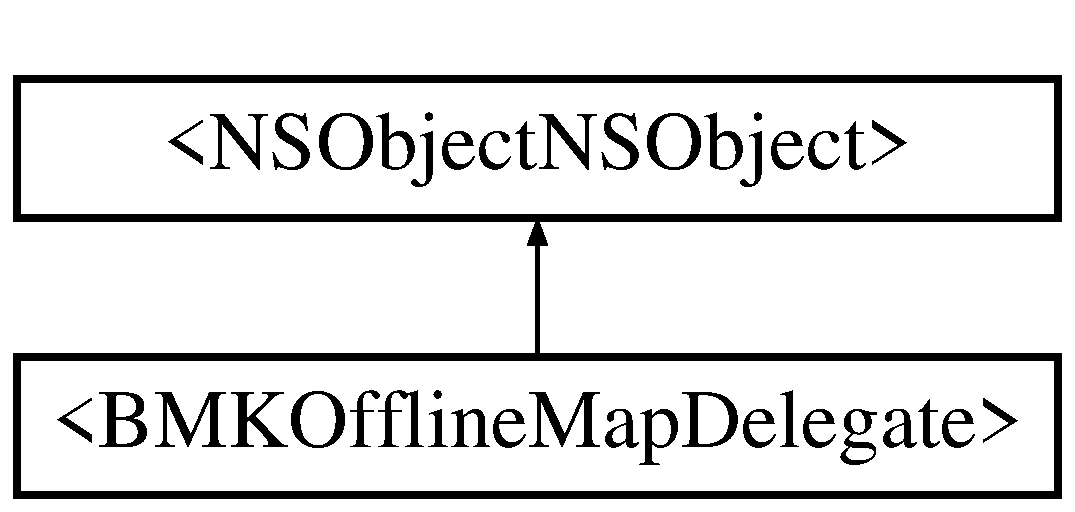
\includegraphics[height=2.000000cm]{protocol_b_m_k_offline_map_delegate-p}
\end{center}
\end{figure}
\subsection*{实例方法}
\begin{DoxyCompactItemize}
\item 
(void) -\/ \hyperlink{protocol_b_m_k_offline_map_delegate-p_abe1dd90ae5ffd9612423c547ab9b1970}{on\-Get\-Offline\-Map\-State\-:with\-State\-:}
\end{DoxyCompactItemize}


\subsection{详细描述}
离线地图delegate,用于获取通知 

\subsection{方法文档}
\hypertarget{protocol_b_m_k_offline_map_delegate-p_abe1dd90ae5ffd9612423c547ab9b1970}{\index{B\-M\-K\-Offline\-Map\-Delegate-\/p@{B\-M\-K\-Offline\-Map\-Delegate-\/p}!on\-Get\-Offline\-Map\-State\-:with\-State\-:@{on\-Get\-Offline\-Map\-State\-:with\-State\-:}}
\index{on\-Get\-Offline\-Map\-State\-:with\-State\-:@{on\-Get\-Offline\-Map\-State\-:with\-State\-:}!BMKOfflineMapDelegate-p@{B\-M\-K\-Offline\-Map\-Delegate-\/p}}
\subsubsection[{on\-Get\-Offline\-Map\-State\-:with\-State\-:}]{\setlength{\rightskip}{0pt plus 5cm}-\/ (void) on\-Get\-Offline\-Map\-State\-: 
\begin{DoxyParamCaption}
\item[{(int)}]{type}
\item[{withState:(int)}]{state}
\end{DoxyParamCaption}
}}\label{protocol_b_m_k_offline_map_delegate-p_abe1dd90ae5ffd9612423c547ab9b1970}
返回通知结果 
\begin{DoxyParams}{参数}
{\em type} & 事件类型: T\-Y\-P\-E\-\_\-\-O\-F\-F\-L\-I\-N\-E\-\_\-\-U\-P\-D\-A\-T\-E,T\-Y\-P\-E\-\_\-\-O\-F\-F\-L\-I\-N\-E\-\_\-\-Z\-I\-P\-C\-N\-T,T\-Y\-P\-E\-\_\-\-O\-F\-F\-L\-I\-N\-E\-\_\-\-U\-N\-Z\-I\-P, T\-Y\-P\-E\-\_\-\-O\-F\-F\-L\-I\-N\-E\-\_\-\-E\-R\-R\-Z\-I\-P, T\-Y\-P\-E\-\_\-\-V\-E\-R\-\_\-\-U\-P\-D\-A\-T\-E, T\-Y\-P\-E\-\_\-\-O\-F\-F\-L\-I\-N\-E\-\_\-\-U\-N\-Z\-I\-P\-F\-I\-N\-I\-S\-H, T\-Y\-P\-E\-\_\-\-O\-F\-F\-L\-I\-N\-E\-\_\-\-A\-D\-D \\
\hline
{\em state} & 事件状态,当type为\-T\-Y\-P\-E\-\_\-\-O\-F\-F\-L\-I\-N\-E\-\_\-\-U\-P\-D\-A\-T\-E时,表示正在下载或更新城市id为state的离线包,当type为\-T\-Y\-P\-E\-\_\-\-O\-F\-F\-L\-I\-N\-E\-\_\-\-Z\-I\-P\-C\-N\-T时,表示检测到state个离线压缩包,当type为\-T\-Y\-P\-E\-\_\-\-O\-F\-F\-L\-I\-N\-E\-\_\-\-A\-D\-D时,表示新安装的离线地图数目,当type为\-T\-Y\-P\-E\-\_\-\-O\-F\-F\-L\-I\-N\-E\-\_\-\-U\-N\-Z\-I\-P时,表示正在解压第state个离线包,当type为\-T\-Y\-P\-E\-\_\-\-O\-F\-F\-L\-I\-N\-E\-\_\-\-E\-R\-R\-Z\-I\-P时,表示有state个错误包,当type为\-T\-Y\-P\-E\-\_\-\-V\-E\-R\-\_\-\-U\-P\-D\-A\-T\-E时,表示id为state的城市离线包有更新,当type为\-T\-Y\-P\-E\-\_\-\-O\-F\-F\-L\-I\-N\-E\-\_\-\-U\-N\-Z\-I\-P\-F\-I\-N\-I\-S\-H时,表示扫瞄完成,成功导入state个离线包 \\
\hline
\end{DoxyParams}


The documentation for this protocol was generated from the following file\-:\begin{DoxyCompactItemize}
\item 
B\-M\-K\-Offline\-Map.\-h\end{DoxyCompactItemize}

\hypertarget{interface_b_m_k_o_l_search_record}{\section{B\-M\-K\-O\-L\-Search\-Record 类参考}
\label{interface_b_m_k_o_l_search_record}\index{B\-M\-K\-O\-L\-Search\-Record@{B\-M\-K\-O\-L\-Search\-Record}}
}


离线地图搜索城市记录结构  




{\ttfamily \#import $<$B\-M\-K\-Offline\-Map\-Type.\-h$>$}

继承关系图 B\-M\-K\-O\-L\-Search\-Record\-:\begin{figure}[H]
\begin{center}
\leavevmode
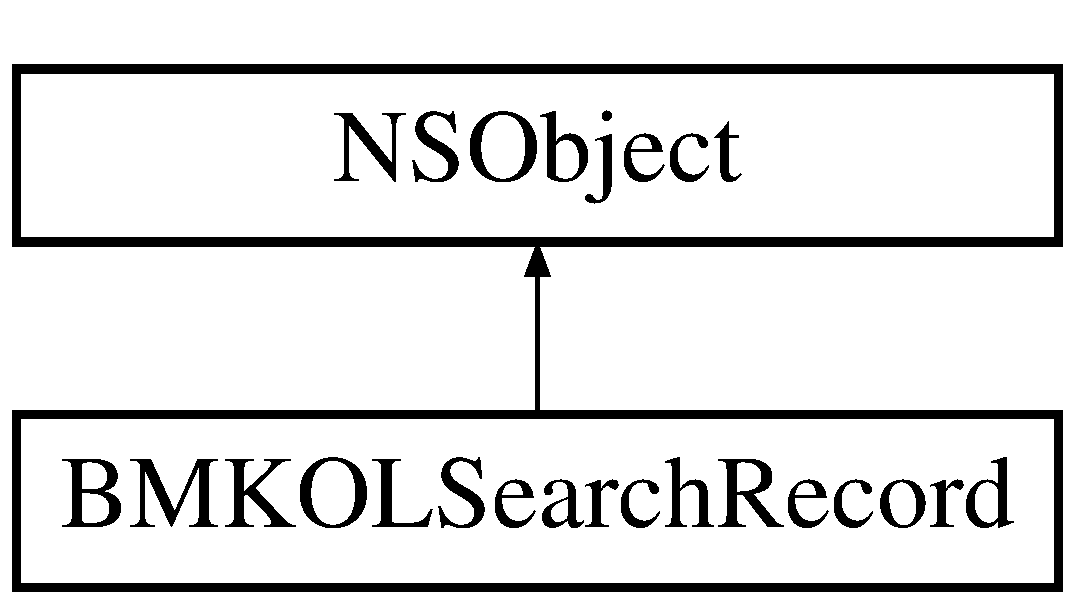
\includegraphics[height=2.000000cm]{interface_b_m_k_o_l_search_record}
\end{center}
\end{figure}
\subsection*{保护成员变量}
\begin{DoxyCompactItemize}
\item 
\hypertarget{interface_b_m_k_o_l_search_record_abb283493e35764e63a41766d40f9f016}{N\-S\-String $\ast$ {\bfseries \-\_\-city\-Name}}\label{interface_b_m_k_o_l_search_record_abb283493e35764e63a41766d40f9f016}

\item 
\hypertarget{interface_b_m_k_o_l_search_record_a16e88995e8c282f3aa7a1dc72cdc9580}{int {\bfseries \-\_\-size}}\label{interface_b_m_k_o_l_search_record_a16e88995e8c282f3aa7a1dc72cdc9580}

\item 
\hypertarget{interface_b_m_k_o_l_search_record_a9ed9011244b41c5360e7d9bd010d7e53}{int {\bfseries \-\_\-city\-I\-D}}\label{interface_b_m_k_o_l_search_record_a9ed9011244b41c5360e7d9bd010d7e53}

\item 
\hypertarget{interface_b_m_k_o_l_search_record_abda23ccbf5aa6fe33911d76a268f013d}{int {\bfseries \-\_\-city\-Type}}\label{interface_b_m_k_o_l_search_record_abda23ccbf5aa6fe33911d76a268f013d}

\item 
\hypertarget{interface_b_m_k_o_l_search_record_a0e6d2797e93de33955702cf362f6ab08}{N\-S\-Array $\ast$ {\bfseries \-\_\-child\-Cities}}\label{interface_b_m_k_o_l_search_record_a0e6d2797e93de33955702cf362f6ab08}

\end{DoxyCompactItemize}
\subsection*{Properties}
\begin{DoxyCompactItemize}
\item 
\hypertarget{interface_b_m_k_o_l_search_record_a9b511c21c21f4b67eef345b11c0e9826}{N\-S\-String $\ast$ \hyperlink{interface_b_m_k_o_l_search_record_a9b511c21c21f4b67eef345b11c0e9826}{city\-Name}}\label{interface_b_m_k_o_l_search_record_a9b511c21c21f4b67eef345b11c0e9826}

\begin{DoxyCompactList}\small\item\em 城市名称 \end{DoxyCompactList}\item 
\hypertarget{interface_b_m_k_o_l_search_record_a65d925120ac45eec0047bad23225f67f}{int \hyperlink{interface_b_m_k_o_l_search_record_a65d925120ac45eec0047bad23225f67f}{size}}\label{interface_b_m_k_o_l_search_record_a65d925120ac45eec0047bad23225f67f}

\begin{DoxyCompactList}\small\item\em 数据包总大小 \end{DoxyCompactList}\item 
\hypertarget{interface_b_m_k_o_l_search_record_a45d36f0768cca26895c7078900ad8d7b}{int \hyperlink{interface_b_m_k_o_l_search_record_a45d36f0768cca26895c7078900ad8d7b}{city\-I\-D}}\label{interface_b_m_k_o_l_search_record_a45d36f0768cca26895c7078900ad8d7b}

\begin{DoxyCompactList}\small\item\em 城市\-I\-D \end{DoxyCompactList}\item 
\hypertarget{interface_b_m_k_o_l_search_record_a74c11b249d3d97503c4a4efa880cc99a}{int \hyperlink{interface_b_m_k_o_l_search_record_a74c11b249d3d97503c4a4efa880cc99a}{city\-Type}}\label{interface_b_m_k_o_l_search_record_a74c11b249d3d97503c4a4efa880cc99a}

\begin{DoxyCompactList}\small\item\em 城市类型 0:全国;1:省份;2:城市;如果是省份,可以通过child\-Cities得到子城市列表 \end{DoxyCompactList}\item 
\hypertarget{interface_b_m_k_o_l_search_record_a883fcb06413f7da8b4e8a50e038a3e78}{N\-S\-Array $\ast$ \hyperlink{interface_b_m_k_o_l_search_record_a883fcb06413f7da8b4e8a50e038a3e78}{child\-Cities}}\label{interface_b_m_k_o_l_search_record_a883fcb06413f7da8b4e8a50e038a3e78}

\begin{DoxyCompactList}\small\item\em 子城市列表 \end{DoxyCompactList}\end{DoxyCompactItemize}


\subsection{详细描述}
离线地图搜索城市记录结构 

The documentation for this class was generated from the following file\-:\begin{DoxyCompactItemize}
\item 
B\-M\-K\-Offline\-Map\-Type.\-h\end{DoxyCompactItemize}

\hypertarget{interface_b_m_k_o_l_update_element}{\section{B\-M\-K\-O\-L\-Update\-Element 类参考}
\label{interface_b_m_k_o_l_update_element}\index{B\-M\-K\-O\-L\-Update\-Element@{B\-M\-K\-O\-L\-Update\-Element}}
}


离线地图更新信息  




{\ttfamily \#import $<$B\-M\-K\-Offline\-Map\-Type.\-h$>$}

继承关系图 B\-M\-K\-O\-L\-Update\-Element\-:\begin{figure}[H]
\begin{center}
\leavevmode
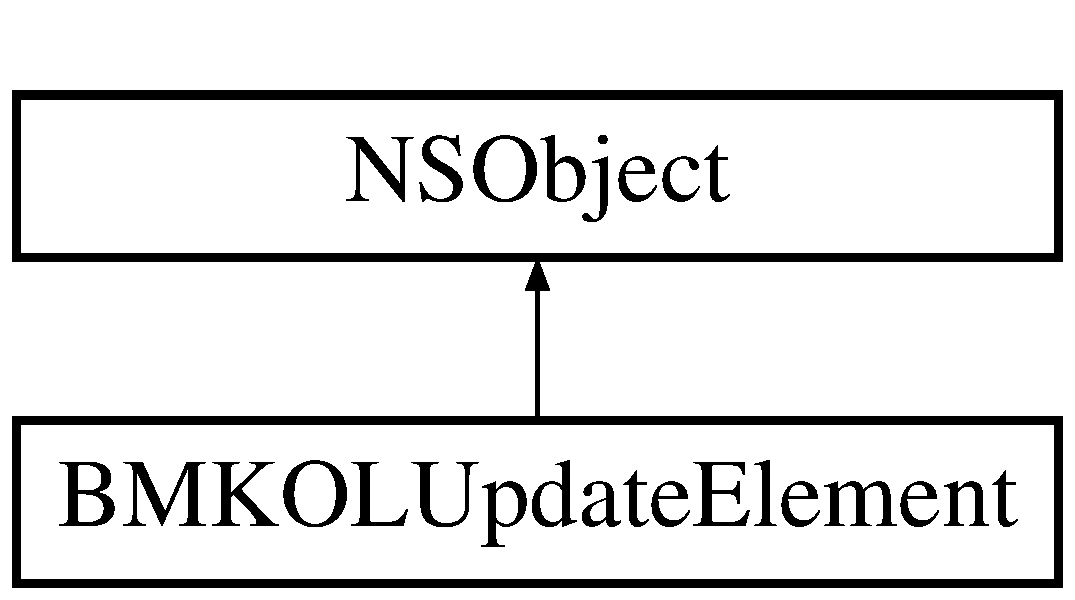
\includegraphics[height=2.000000cm]{interface_b_m_k_o_l_update_element}
\end{center}
\end{figure}
\subsection*{保护成员变量}
\begin{DoxyCompactItemize}
\item 
\hypertarget{interface_b_m_k_o_l_update_element_aa136416d4cc93c840d971046171358f3}{int {\bfseries \-\_\-city\-I\-D}}\label{interface_b_m_k_o_l_update_element_aa136416d4cc93c840d971046171358f3}

\item 
\hypertarget{interface_b_m_k_o_l_update_element_a9b77aeb4ed08740f3dab046fb48cf4f9}{int {\bfseries \-\_\-size}}\label{interface_b_m_k_o_l_update_element_a9b77aeb4ed08740f3dab046fb48cf4f9}

\item 
\hypertarget{interface_b_m_k_o_l_update_element_acf85b01f08fccf6e7ab5d1bbce6485b6}{int {\bfseries \-\_\-serversize}}\label{interface_b_m_k_o_l_update_element_acf85b01f08fccf6e7ab5d1bbce6485b6}

\item 
\hypertarget{interface_b_m_k_o_l_update_element_a2ce86cc25a0ce594be9dee2ed7ed6d7b}{B\-O\-O\-L {\bfseries \-\_\-update}}\label{interface_b_m_k_o_l_update_element_a2ce86cc25a0ce594be9dee2ed7ed6d7b}

\item 
\hypertarget{interface_b_m_k_o_l_update_element_a7d22cf3754355f93fb119984121d25be}{int {\bfseries \-\_\-ratio}}\label{interface_b_m_k_o_l_update_element_a7d22cf3754355f93fb119984121d25be}

\item 
\hypertarget{interface_b_m_k_o_l_update_element_afac492949ec4ce5f4f229de43f9a6836}{int {\bfseries \-\_\-status}}\label{interface_b_m_k_o_l_update_element_afac492949ec4ce5f4f229de43f9a6836}

\item 
\hypertarget{interface_b_m_k_o_l_update_element_a21210d50957c6b1ebddd9f5bdfed5e7f}{C\-L\-Location\-Coordinate2\-D {\bfseries \-\_\-pt}}\label{interface_b_m_k_o_l_update_element_a21210d50957c6b1ebddd9f5bdfed5e7f}

\end{DoxyCompactItemize}
\subsection*{Properties}
\begin{DoxyCompactItemize}
\item 
\hypertarget{interface_b_m_k_o_l_update_element_aa27dfbfc8e801d04ea9a55c43793fe24}{N\-S\-String $\ast$ {\bfseries \-\_\-city\-Name}}\label{interface_b_m_k_o_l_update_element_aa27dfbfc8e801d04ea9a55c43793fe24}

\item 
\hypertarget{interface_b_m_k_o_l_update_element_acf8998f896d5eee3bf25b5efaf316ffa}{N\-S\-String $\ast$ \hyperlink{interface_b_m_k_o_l_update_element_acf8998f896d5eee3bf25b5efaf316ffa}{city\-Name}}\label{interface_b_m_k_o_l_update_element_acf8998f896d5eee3bf25b5efaf316ffa}

\begin{DoxyCompactList}\small\item\em 城市名称 \end{DoxyCompactList}\item 
\hypertarget{interface_b_m_k_o_l_update_element_a0fc2ac335466b2fb891d1c3c430e14db}{int \hyperlink{interface_b_m_k_o_l_update_element_a0fc2ac335466b2fb891d1c3c430e14db}{city\-I\-D}}\label{interface_b_m_k_o_l_update_element_a0fc2ac335466b2fb891d1c3c430e14db}

\begin{DoxyCompactList}\small\item\em 城市\-I\-D \end{DoxyCompactList}\item 
\hypertarget{interface_b_m_k_o_l_update_element_a64207ce9d00c3127b02fbeaeb2dfc49c}{int \hyperlink{interface_b_m_k_o_l_update_element_a64207ce9d00c3127b02fbeaeb2dfc49c}{size}}\label{interface_b_m_k_o_l_update_element_a64207ce9d00c3127b02fbeaeb2dfc49c}

\begin{DoxyCompactList}\small\item\em 已下载数据大小,单位:字节 \end{DoxyCompactList}\item 
\hypertarget{interface_b_m_k_o_l_update_element_ad61b9f37f09ee7c2c2c41570c1329d1e}{int \hyperlink{interface_b_m_k_o_l_update_element_ad61b9f37f09ee7c2c2c41570c1329d1e}{serversize}}\label{interface_b_m_k_o_l_update_element_ad61b9f37f09ee7c2c2c41570c1329d1e}

\begin{DoxyCompactList}\small\item\em 服务端数据大小,当update为\-Y\-E\-S时有效,单位:字节 \end{DoxyCompactList}\item 
\hypertarget{interface_b_m_k_o_l_update_element_a8f26b0d8b91573b17f2314fe5795dcd4}{int \hyperlink{interface_b_m_k_o_l_update_element_a8f26b0d8b91573b17f2314fe5795dcd4}{ratio}}\label{interface_b_m_k_o_l_update_element_a8f26b0d8b91573b17f2314fe5795dcd4}

\begin{DoxyCompactList}\small\item\em 下载比率,100为下载完成 \end{DoxyCompactList}\item 
\hypertarget{interface_b_m_k_o_l_update_element_a1e980d13929fc0dc732edddf1ae13bf2}{int \hyperlink{interface_b_m_k_o_l_update_element_a1e980d13929fc0dc732edddf1ae13bf2}{status}}\label{interface_b_m_k_o_l_update_element_a1e980d13929fc0dc732edddf1ae13bf2}

\begin{DoxyCompactList}\small\item\em 下载状态, 1\-:正在下载 2\-:等待下载 3\-:已暂停 4\-:完成 \end{DoxyCompactList}\item 
\hypertarget{interface_b_m_k_o_l_update_element_a1adc137eba11d9ae142310d3556bc446}{B\-O\-O\-L \hyperlink{interface_b_m_k_o_l_update_element_a1adc137eba11d9ae142310d3556bc446}{update}}\label{interface_b_m_k_o_l_update_element_a1adc137eba11d9ae142310d3556bc446}

\begin{DoxyCompactList}\small\item\em 更新状态 \end{DoxyCompactList}\item 
\hypertarget{interface_b_m_k_o_l_update_element_a9e229b507ced476146db8f80c71ea5bd}{C\-L\-Location\-Coordinate2\-D \hyperlink{interface_b_m_k_o_l_update_element_a9e229b507ced476146db8f80c71ea5bd}{pt}}\label{interface_b_m_k_o_l_update_element_a9e229b507ced476146db8f80c71ea5bd}

\begin{DoxyCompactList}\small\item\em 城市中心点 \end{DoxyCompactList}\end{DoxyCompactItemize}


\subsection{详细描述}
离线地图更新信息 

The documentation for this class was generated from the following file\-:\begin{DoxyCompactItemize}
\item 
B\-M\-K\-Offline\-Map\-Type.\-h\end{DoxyCompactItemize}

\hypertarget{protocol_b_m_k_overlay-p}{\section{$<$B\-M\-K\-Overlay$>$ 协议参考}
\label{protocol_b_m_k_overlay-p}\index{$<$\-B\-M\-K\-Overlay$>$@{$<$\-B\-M\-K\-Overlay$>$}}
}


该类是地图覆盖物的基类,所有地图的覆盖物需要继承自此类  




{\ttfamily \#import $<$B\-M\-K\-Overlay.\-h$>$}

继承关系图 $<$B\-M\-K\-Overlay$>$\-:\begin{figure}[H]
\begin{center}
\leavevmode
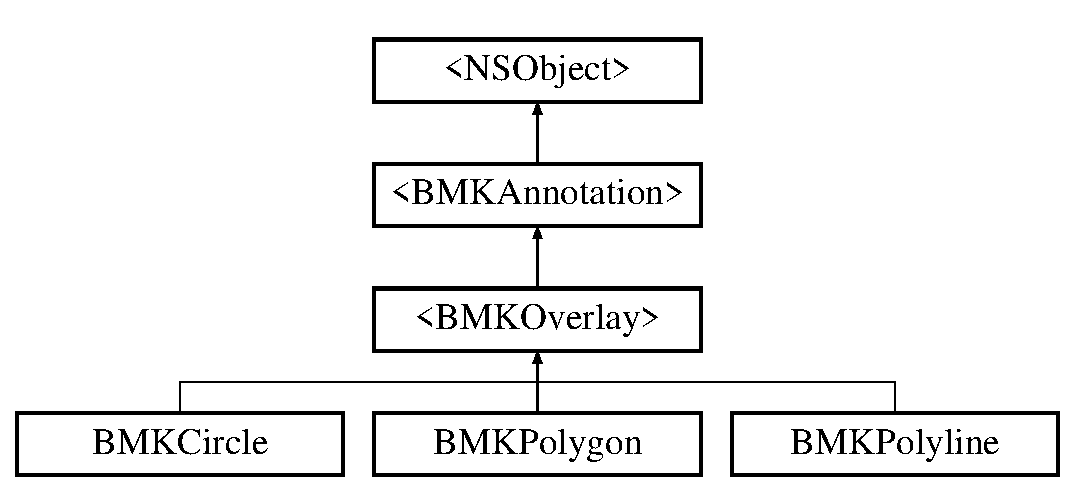
\includegraphics[height=4.000000cm]{protocol_b_m_k_overlay-p}
\end{center}
\end{figure}
\subsection*{实例方法}
\begin{DoxyCompactItemize}
\item 
(B\-O\-O\-L) -\/ \hyperlink{protocol_b_m_k_overlay-p_ad89c522da656c2a977b87bdc1cc4bf21}{intersects\-Map\-Rect\-:}
\end{DoxyCompactItemize}
\subsection*{Properties}
\begin{DoxyCompactItemize}
\item 
\hypertarget{protocol_b_m_k_overlay-p_a7a10d9dde65c9611e3b5279179a9d480}{C\-L\-Location\-Coordinate2\-D \hyperlink{protocol_b_m_k_overlay-p_a7a10d9dde65c9611e3b5279179a9d480}{coordinate}}\label{protocol_b_m_k_overlay-p_a7a10d9dde65c9611e3b5279179a9d480}

\begin{DoxyCompactList}\small\item\em 返回区域中心坐标. \end{DoxyCompactList}\item 
\hypertarget{protocol_b_m_k_overlay-p_a77465daa9e52be51cc5aa15591ab74f0}{\hyperlink{struct_b_m_k_map_rect}{B\-M\-K\-Map\-Rect} \hyperlink{protocol_b_m_k_overlay-p_a77465daa9e52be51cc5aa15591ab74f0}{bounding\-Map\-Rect}}\label{protocol_b_m_k_overlay-p_a77465daa9e52be51cc5aa15591ab74f0}

\begin{DoxyCompactList}\small\item\em 返回区域外接矩形 \end{DoxyCompactList}\end{DoxyCompactItemize}


\subsection{详细描述}
该类是地图覆盖物的基类,所有地图的覆盖物需要继承自此类 

\subsection{方法文档}
\hypertarget{protocol_b_m_k_overlay-p_ad89c522da656c2a977b87bdc1cc4bf21}{\index{B\-M\-K\-Overlay-\/p@{B\-M\-K\-Overlay-\/p}!intersects\-Map\-Rect\-:@{intersects\-Map\-Rect\-:}}
\index{intersects\-Map\-Rect\-:@{intersects\-Map\-Rect\-:}!BMKOverlay-p@{B\-M\-K\-Overlay-\/p}}
\subsubsection[{intersects\-Map\-Rect\-:}]{\setlength{\rightskip}{0pt plus 5cm}-\/ (B\-O\-O\-L) intersects\-Map\-Rect\-: 
\begin{DoxyParamCaption}
\item[{({\bf B\-M\-K\-Map\-Rect})}]{map\-Rect}
\end{DoxyParamCaption}
\hspace{0.3cm}{\ttfamily [optional]}}}\label{protocol_b_m_k_overlay-p_ad89c522da656c2a977b87bdc1cc4bf21}
判断指定的矩形是否与本\-Overlay相交,用于更精确的控制overlay view的显示. 默认使用\-B\-M\-K\-Map\-Rect\-Intersects\-Rect(\mbox{[}overlay bounding\-Rect\mbox{]}, map\-Rect)代替. 
\begin{DoxyParams}{参数}
{\em map\-Rect} & 指定的\-B\-M\-K\-Map\-Rect \\
\hline
\end{DoxyParams}
\begin{DoxyReturn}{返回}
如果相交返回\-Y\-E\-S,否则返回\-N\-O 
\end{DoxyReturn}


The documentation for this protocol was generated from the following file\-:\begin{DoxyCompactItemize}
\item 
B\-M\-K\-Overlay.\-h\end{DoxyCompactItemize}

\hypertarget{interface_b_m_k_overlay_path_view}{\section{B\-M\-K\-Overlay\-Path\-View 类参考}
\label{interface_b_m_k_overlay_path_view}\index{B\-M\-K\-Overlay\-Path\-View@{B\-M\-K\-Overlay\-Path\-View}}
}


该类定义了一个基本的\-Overlay\-View,并且在\-B\-Map\-Kit中预置了几个经常使用的\-Overlay\-View  




{\ttfamily \#import $<$B\-M\-K\-Overlay\-Path\-View.\-h$>$}

继承关系图 B\-M\-K\-Overlay\-Path\-View\-:\begin{figure}[H]
\begin{center}
\leavevmode
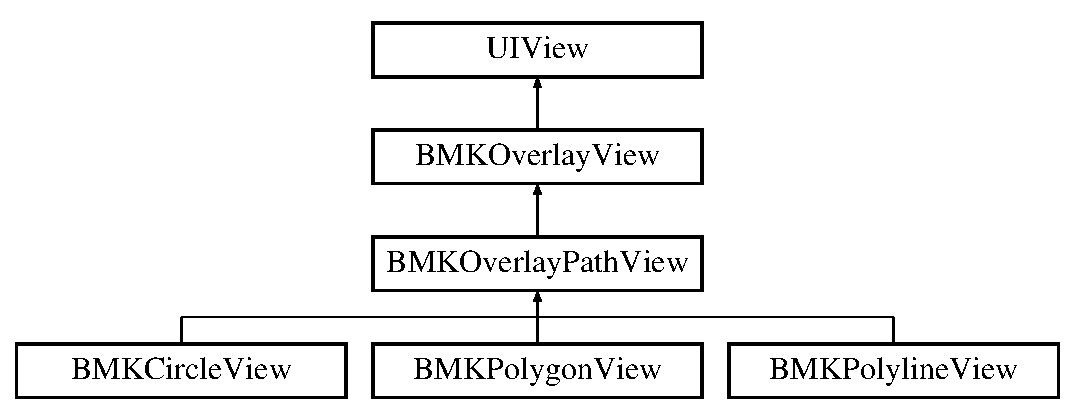
\includegraphics[height=4.000000cm]{interface_b_m_k_overlay_path_view}
\end{center}
\end{figure}
\subsection*{实例方法}
\begin{DoxyCompactItemize}
\item 
(void) -\/ \hyperlink{interface_b_m_k_overlay_path_view_a4e76c3b9524b555c2118ae18f6057605}{create\-Path}
\item 
(void) -\/ \hyperlink{interface_b_m_k_overlay_path_view_ac773bae0823405dcf5b78a3361fa2d56}{invalidate\-Path}
\item 
(void) -\/ \hyperlink{interface_b_m_k_overlay_path_view_a2acbf6bd9401c2904148b7b6cf85c6e9}{apply\-Stroke\-Properties\-To\-Context\-:at\-Zoom\-Scale\-:}
\item 
(void) -\/ \hyperlink{interface_b_m_k_overlay_path_view_af549bea37a94164a088826f9a962e08c}{apply\-Fill\-Properties\-To\-Context\-:at\-Zoom\-Scale\-:}
\item 
(void) -\/ \hyperlink{interface_b_m_k_overlay_path_view_a482e5fe24f04335d090b32d449ef6dc4}{stroke\-Path\-:in\-Context\-:}
\item 
(void) -\/ \hyperlink{interface_b_m_k_overlay_path_view_a036abde24b9ae921f209cde884dad49b}{fill\-Path\-:in\-Context\-:}
\end{DoxyCompactItemize}
\subsection*{保护成员变量}
\begin{DoxyCompactItemize}
\item 
\hypertarget{interface_b_m_k_overlay_path_view_acc3564ea23047d84cc7656ce15c8d393}{package U\-I\-Color $\ast$ {\bfseries \-\_\-fill\-Color}}\label{interface_b_m_k_overlay_path_view_acc3564ea23047d84cc7656ce15c8d393}

\item 
\hypertarget{interface_b_m_k_overlay_path_view_a3e288997d3aa85a36d35a437cc6f9198}{U\-I\-Color $\ast$ {\bfseries \-\_\-stroke\-Color}}\label{interface_b_m_k_overlay_path_view_a3e288997d3aa85a36d35a437cc6f9198}

\item 
\hypertarget{interface_b_m_k_overlay_path_view_a09255527f57e864e0bd2a908f87789de}{C\-G\-Float {\bfseries \-\_\-line\-Width}}\label{interface_b_m_k_overlay_path_view_a09255527f57e864e0bd2a908f87789de}

\item 
\hypertarget{interface_b_m_k_overlay_path_view_a46d7a15cc3e746c7e318d38525dc15ee}{C\-G\-Line\-Join {\bfseries \-\_\-line\-Join}}\label{interface_b_m_k_overlay_path_view_a46d7a15cc3e746c7e318d38525dc15ee}

\item 
\hypertarget{interface_b_m_k_overlay_path_view_a69ebe48069dfc67a636d6ec39eed87d7}{C\-G\-Line\-Cap {\bfseries \-\_\-line\-Cap}}\label{interface_b_m_k_overlay_path_view_a69ebe48069dfc67a636d6ec39eed87d7}

\item 
\hypertarget{interface_b_m_k_overlay_path_view_a26c31e09cfce21dd87bb1a838fee6d93}{C\-G\-Float {\bfseries \-\_\-miter\-Limit}}\label{interface_b_m_k_overlay_path_view_a26c31e09cfce21dd87bb1a838fee6d93}

\item 
\hypertarget{interface_b_m_k_overlay_path_view_afc1d60d9090890522425fe8e66295c43}{C\-G\-Float {\bfseries \-\_\-line\-Dash\-Phase}}\label{interface_b_m_k_overlay_path_view_afc1d60d9090890522425fe8e66295c43}

\item 
\hypertarget{interface_b_m_k_overlay_path_view_a272a0cd6bdb5b7a693f7169d0b5168e7}{N\-S\-Array $\ast$ {\bfseries \-\_\-line\-Dash\-Pattern}}\label{interface_b_m_k_overlay_path_view_a272a0cd6bdb5b7a693f7169d0b5168e7}

\item 
\hypertarget{interface_b_m_k_overlay_path_view_a803f7a80f30080739fe2d853819374dd}{C\-G\-Path\-Ref {\bfseries \-\_\-path}}\label{interface_b_m_k_overlay_path_view_a803f7a80f30080739fe2d853819374dd}

\end{DoxyCompactItemize}
\subsection*{Properties}
\begin{DoxyCompactItemize}
\item 
\hypertarget{interface_b_m_k_overlay_path_view_a955c1cfe9de3338eccbde829a6651d07}{U\-I\-Color $\ast$ \hyperlink{interface_b_m_k_overlay_path_view_a955c1cfe9de3338eccbde829a6651d07}{fill\-Color}}\label{interface_b_m_k_overlay_path_view_a955c1cfe9de3338eccbde829a6651d07}

\begin{DoxyCompactList}\small\item\em 填充颜色 \end{DoxyCompactList}\item 
\hypertarget{interface_b_m_k_overlay_path_view_a5fe2c3236a16a520f9f867bd34dac08e}{U\-I\-Color $\ast$ \hyperlink{interface_b_m_k_overlay_path_view_a5fe2c3236a16a520f9f867bd34dac08e}{stroke\-Color}}\label{interface_b_m_k_overlay_path_view_a5fe2c3236a16a520f9f867bd34dac08e}

\begin{DoxyCompactList}\small\item\em 画笔颜色 \end{DoxyCompactList}\item 
\hypertarget{interface_b_m_k_overlay_path_view_a037ec8a5e6c8ee0f9b6459c8dbe280bb}{C\-G\-Float \hyperlink{interface_b_m_k_overlay_path_view_a037ec8a5e6c8ee0f9b6459c8dbe280bb}{line\-Width}}\label{interface_b_m_k_overlay_path_view_a037ec8a5e6c8ee0f9b6459c8dbe280bb}

\begin{DoxyCompactList}\small\item\em 画笔宽度,默认为0 \end{DoxyCompactList}\item 
\hypertarget{interface_b_m_k_overlay_path_view_aa57813af69de6d1852f47cdc198393fc}{C\-G\-Line\-Join \hyperlink{interface_b_m_k_overlay_path_view_aa57813af69de6d1852f47cdc198393fc}{line\-Join}}\label{interface_b_m_k_overlay_path_view_aa57813af69de6d1852f47cdc198393fc}

\begin{DoxyCompactList}\small\item\em Line\-Join,默认为k\-C\-G\-Line\-Join\-Round. \end{DoxyCompactList}\item 
\hypertarget{interface_b_m_k_overlay_path_view_a3b52405ce16992ffd75e98cf7f8392a1}{C\-G\-Line\-Cap \hyperlink{interface_b_m_k_overlay_path_view_a3b52405ce16992ffd75e98cf7f8392a1}{line\-Cap}}\label{interface_b_m_k_overlay_path_view_a3b52405ce16992ffd75e98cf7f8392a1}

\begin{DoxyCompactList}\small\item\em Line\-Cap,默认为k\-C\-G\-Line\-Cap\-Round. \end{DoxyCompactList}\item 
\hypertarget{interface_b_m_k_overlay_path_view_a097b8a404bc074f802b7dcba593bdd40}{C\-G\-Float \hyperlink{interface_b_m_k_overlay_path_view_a097b8a404bc074f802b7dcba593bdd40}{miter\-Limit}}\label{interface_b_m_k_overlay_path_view_a097b8a404bc074f802b7dcba593bdd40}

\begin{DoxyCompactList}\small\item\em miter\-Limit,在样式为k\-C\-G\-Line\-Join\-Miter时有效,默认为10 \end{DoxyCompactList}\item 
\hypertarget{interface_b_m_k_overlay_path_view_ab1b6a4d757514e534fa76c92faf5270f}{C\-G\-Float \hyperlink{interface_b_m_k_overlay_path_view_ab1b6a4d757514e534fa76c92faf5270f}{line\-Dash\-Phase}}\label{interface_b_m_k_overlay_path_view_ab1b6a4d757514e534fa76c92faf5270f}

\begin{DoxyCompactList}\small\item\em line\-Dash\-Phase, 默认为0 \end{DoxyCompactList}\item 
\hypertarget{interface_b_m_k_overlay_path_view_aa8064f10fe64961b37efb2dadeb83b8d}{N\-S\-Array $\ast$ \hyperlink{interface_b_m_k_overlay_path_view_aa8064f10fe64961b37efb2dadeb83b8d}{line\-Dash\-Pattern}}\label{interface_b_m_k_overlay_path_view_aa8064f10fe64961b37efb2dadeb83b8d}

\begin{DoxyCompactList}\small\item\em line\-Dash\-Pattern,一个\-N\-S\-Numbers的数组,默认为nil \end{DoxyCompactList}\item 
\hypertarget{interface_b_m_k_overlay_path_view_a0e1316ba1283dcc2a772a9489efac73b}{C\-G\-Path\-Ref \hyperlink{interface_b_m_k_overlay_path_view_a0e1316ba1283dcc2a772a9489efac73b}{path}}\label{interface_b_m_k_overlay_path_view_a0e1316ba1283dcc2a772a9489efac73b}

\begin{DoxyCompactList}\small\item\em path对象 \end{DoxyCompactList}\end{DoxyCompactItemize}


\subsection{详细描述}
该类定义了一个基本的\-Overlay\-View,并且在\-B\-Map\-Kit中预置了几个经常使用的\-Overlay\-View 

\subsection{方法文档}
\hypertarget{interface_b_m_k_overlay_path_view_af549bea37a94164a088826f9a962e08c}{\index{B\-M\-K\-Overlay\-Path\-View@{B\-M\-K\-Overlay\-Path\-View}!apply\-Fill\-Properties\-To\-Context\-:at\-Zoom\-Scale\-:@{apply\-Fill\-Properties\-To\-Context\-:at\-Zoom\-Scale\-:}}
\index{apply\-Fill\-Properties\-To\-Context\-:at\-Zoom\-Scale\-:@{apply\-Fill\-Properties\-To\-Context\-:at\-Zoom\-Scale\-:}!BMKOverlayPathView@{B\-M\-K\-Overlay\-Path\-View}}
\subsubsection[{apply\-Fill\-Properties\-To\-Context\-:at\-Zoom\-Scale\-:}]{\setlength{\rightskip}{0pt plus 5cm}-\/ (void) apply\-Fill\-Properties\-To\-Context\-: 
\begin{DoxyParamCaption}
\item[{(C\-G\-Context\-Ref)}]{context}
\item[{atZoomScale:({\bf B\-M\-K\-Zoom\-Scale})}]{zoom\-Scale}
\end{DoxyParamCaption}
}}\label{interface_b_m_k_overlay_path_view_af549bea37a94164a088826f9a962e08c}
应用画刷属性 
\begin{DoxyParams}{参数}
{\em context} & C\-G\-Context对象 \\
\hline
{\em zoom\-Scale} & 当前的zoom\-Scale \\
\hline
\end{DoxyParams}
\hypertarget{interface_b_m_k_overlay_path_view_a2acbf6bd9401c2904148b7b6cf85c6e9}{\index{B\-M\-K\-Overlay\-Path\-View@{B\-M\-K\-Overlay\-Path\-View}!apply\-Stroke\-Properties\-To\-Context\-:at\-Zoom\-Scale\-:@{apply\-Stroke\-Properties\-To\-Context\-:at\-Zoom\-Scale\-:}}
\index{apply\-Stroke\-Properties\-To\-Context\-:at\-Zoom\-Scale\-:@{apply\-Stroke\-Properties\-To\-Context\-:at\-Zoom\-Scale\-:}!BMKOverlayPathView@{B\-M\-K\-Overlay\-Path\-View}}
\subsubsection[{apply\-Stroke\-Properties\-To\-Context\-:at\-Zoom\-Scale\-:}]{\setlength{\rightskip}{0pt plus 5cm}-\/ (void) apply\-Stroke\-Properties\-To\-Context\-: 
\begin{DoxyParamCaption}
\item[{(C\-G\-Context\-Ref)}]{context}
\item[{atZoomScale:({\bf B\-M\-K\-Zoom\-Scale})}]{zoom\-Scale}
\end{DoxyParamCaption}
}}\label{interface_b_m_k_overlay_path_view_a2acbf6bd9401c2904148b7b6cf85c6e9}
应用画笔属性 
\begin{DoxyParams}{参数}
{\em context} & C\-G\-Context对象 \\
\hline
{\em zoom\-Scale} & 当前的zoom\-Scale \\
\hline
\end{DoxyParams}
\hypertarget{interface_b_m_k_overlay_path_view_a4e76c3b9524b555c2118ae18f6057605}{\index{B\-M\-K\-Overlay\-Path\-View@{B\-M\-K\-Overlay\-Path\-View}!create\-Path@{create\-Path}}
\index{create\-Path@{create\-Path}!BMKOverlayPathView@{B\-M\-K\-Overlay\-Path\-View}}
\subsubsection[{create\-Path}]{\setlength{\rightskip}{0pt plus 5cm}-\/ (void) create\-Path 
\begin{DoxyParamCaption}
{}
\end{DoxyParamCaption}
}}\label{interface_b_m_k_overlay_path_view_a4e76c3b9524b555c2118ae18f6057605}
生成要绘制的path,子类需要重写此函数,并且对path属性赋值:self.\-path = new\-Path; \hypertarget{interface_b_m_k_overlay_path_view_a036abde24b9ae921f209cde884dad49b}{\index{B\-M\-K\-Overlay\-Path\-View@{B\-M\-K\-Overlay\-Path\-View}!fill\-Path\-:in\-Context\-:@{fill\-Path\-:in\-Context\-:}}
\index{fill\-Path\-:in\-Context\-:@{fill\-Path\-:in\-Context\-:}!BMKOverlayPathView@{B\-M\-K\-Overlay\-Path\-View}}
\subsubsection[{fill\-Path\-:in\-Context\-:}]{\setlength{\rightskip}{0pt plus 5cm}-\/ (void) fill\-Path\-: 
\begin{DoxyParamCaption}
\item[{(C\-G\-Path\-Ref)}]{path}
\item[{inContext:(C\-G\-Context\-Ref)}]{context}
\end{DoxyParamCaption}
}}\label{interface_b_m_k_overlay_path_view_a036abde24b9ae921f209cde884dad49b}
填充path 
\begin{DoxyParams}{参数}
{\em path} & 要绘制的\-C\-G\-Path \\
\hline
{\em context} & C\-G\-Context对象 \\
\hline
\end{DoxyParams}
\hypertarget{interface_b_m_k_overlay_path_view_ac773bae0823405dcf5b78a3361fa2d56}{\index{B\-M\-K\-Overlay\-Path\-View@{B\-M\-K\-Overlay\-Path\-View}!invalidate\-Path@{invalidate\-Path}}
\index{invalidate\-Path@{invalidate\-Path}!BMKOverlayPathView@{B\-M\-K\-Overlay\-Path\-View}}
\subsubsection[{invalidate\-Path}]{\setlength{\rightskip}{0pt plus 5cm}-\/ (void) invalidate\-Path 
\begin{DoxyParamCaption}
{}
\end{DoxyParamCaption}
}}\label{interface_b_m_k_overlay_path_view_ac773bae0823405dcf5b78a3361fa2d56}
刷新path,调用该函数将会使已经缓存的path失效,将会重新调用create\-Path来生成新的path对象 \hypertarget{interface_b_m_k_overlay_path_view_a482e5fe24f04335d090b32d449ef6dc4}{\index{B\-M\-K\-Overlay\-Path\-View@{B\-M\-K\-Overlay\-Path\-View}!stroke\-Path\-:in\-Context\-:@{stroke\-Path\-:in\-Context\-:}}
\index{stroke\-Path\-:in\-Context\-:@{stroke\-Path\-:in\-Context\-:}!BMKOverlayPathView@{B\-M\-K\-Overlay\-Path\-View}}
\subsubsection[{stroke\-Path\-:in\-Context\-:}]{\setlength{\rightskip}{0pt plus 5cm}-\/ (void) stroke\-Path\-: 
\begin{DoxyParamCaption}
\item[{(C\-G\-Path\-Ref)}]{path}
\item[{inContext:(C\-G\-Context\-Ref)}]{context}
\end{DoxyParamCaption}
}}\label{interface_b_m_k_overlay_path_view_a482e5fe24f04335d090b32d449ef6dc4}
绘制path 
\begin{DoxyParams}{参数}
{\em path} & 要绘制的\-C\-G\-Path \\
\hline
{\em context} & C\-G\-Context对象 \\
\hline
\end{DoxyParams}


The documentation for this class was generated from the following file\-:\begin{DoxyCompactItemize}
\item 
B\-M\-K\-Overlay\-Path\-View.\-h\end{DoxyCompactItemize}

\hypertarget{interface_b_m_k_overlay_view}{\section{B\-M\-K\-Overlay\-View 类参考}
\label{interface_b_m_k_overlay_view}\index{B\-M\-K\-Overlay\-View@{B\-M\-K\-Overlay\-View}}
}


该类是地图覆盖物\-View的基类,提供绘制overlay的接口但本身并无实现,所有地图覆盖物\-View需要继承自此类  




{\ttfamily \#import $<$B\-M\-K\-Overlay\-View.\-h$>$}

继承关系图 B\-M\-K\-Overlay\-View\-:\begin{figure}[H]
\begin{center}
\leavevmode
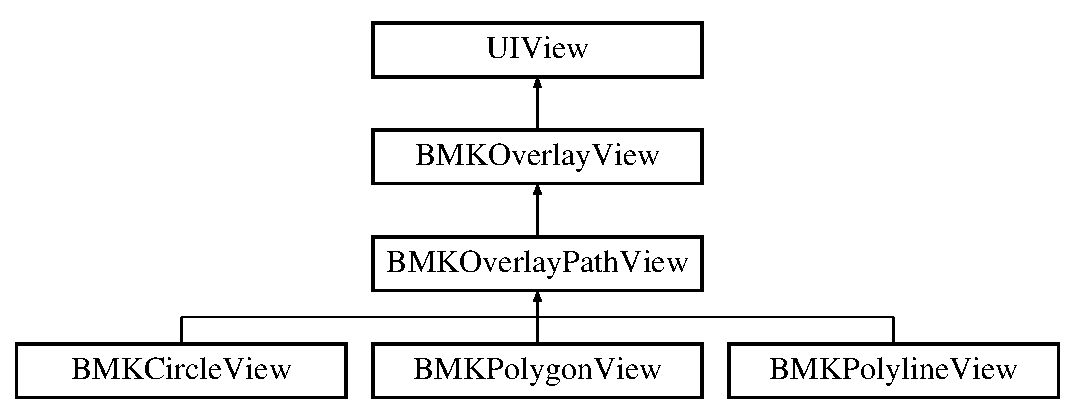
\includegraphics[height=4.000000cm]{interface_b_m_k_overlay_view}
\end{center}
\end{figure}
\subsection*{实例方法}
\begin{DoxyCompactItemize}
\item 
(id) -\/ \hyperlink{interface_b_m_k_overlay_view_a93cdba852e915d6a417b95edabe4af4c}{init\-With\-Overlay\-:}
\item 
(C\-G\-Point) -\/ \hyperlink{interface_b_m_k_overlay_view_a211d0d55b1c10b0abca45e83f4fcf05c}{point\-For\-Map\-Point\-:}
\item 
(\hyperlink{struct_b_m_k_map_point}{B\-M\-K\-Map\-Point}) -\/ \hyperlink{interface_b_m_k_overlay_view_ab0270107a383cf49fd46d9b624604d53}{map\-Point\-For\-Point\-:}
\item 
(C\-G\-Rect) -\/ \hyperlink{interface_b_m_k_overlay_view_a4eb52fd9951bcfc898e9a026ee40e99e}{rect\-For\-Map\-Rect\-:}
\item 
(\hyperlink{struct_b_m_k_map_rect}{B\-M\-K\-Map\-Rect}) -\/ \hyperlink{interface_b_m_k_overlay_view_ae8c0f0415357f281451eaa602b3f388b}{map\-Rect\-For\-Rect\-:}
\item 
(B\-O\-O\-L) -\/ \hyperlink{interface_b_m_k_overlay_view_ad5c0685243ded79bc6657ebb7df08f87}{can\-Draw\-Map\-Rect\-:zoom\-Scale\-:}
\item 
(void) -\/ \hyperlink{interface_b_m_k_overlay_view_aad771b4c325461d99b142e79287188dc}{draw\-Map\-Rect\-:zoom\-Scale\-:in\-Context\-:}
\item 
(void) -\/ \hyperlink{interface_b_m_k_overlay_view_aca005b8bf49d57b404da473fd6f0d534}{set\-Needs\-Display\-In\-Map\-Rect\-:}
\item 
(void) -\/ \hyperlink{interface_b_m_k_overlay_view_a67fcc048446dfa1725aa4a86b241b282}{render\-Lines\-With\-Points\-:point\-Count\-:stroke\-Color\-:line\-Width\-:looped\-:}
\item 
(void) -\/ \hyperlink{interface_b_m_k_overlay_view_a85a054df49b09373b036e22771138ba2}{render\-Region\-With\-Points\-:point\-Count\-:fill\-Color\-:using\-Triangle\-Fan\-:}
\item 
(void) -\/ \hyperlink{interface_b_m_k_overlay_view_a0a851a886a4bb7268ea595d3892ab59f}{gl\-Render}
\end{DoxyCompactItemize}
\subsection*{保护成员变量}
\begin{DoxyCompactItemize}
\item 
\hypertarget{interface_b_m_k_overlay_view_a1221418aafb1e98ab9caf88bb5fea5d7}{package id$<$ \hyperlink{protocol_b_m_k_overlay-p}{B\-M\-K\-Overlay} $>$ {\bfseries \-\_\-overlay}}\label{interface_b_m_k_overlay_view_a1221418aafb1e98ab9caf88bb5fea5d7}

\item 
\hypertarget{interface_b_m_k_overlay_view_a9c358f158a9d30b23ff8dddce028be61}{\hyperlink{struct_b_m_k_map_rect}{B\-M\-K\-Map\-Rect} {\bfseries \-\_\-bounding\-Map\-Rect}}\label{interface_b_m_k_overlay_view_a9c358f158a9d30b23ff8dddce028be61}

\item 
\hypertarget{interface_b_m_k_overlay_view_a33718c9269f4aad056f2360a368d65bb}{C\-G\-Affine\-Transform {\bfseries \-\_\-map\-Transform}}\label{interface_b_m_k_overlay_view_a33718c9269f4aad056f2360a368d65bb}

\item 
\hypertarget{interface_b_m_k_overlay_view_a811bdb8cdb5c83a3e91674eeb35db281}{id {\bfseries \-\_\-geometry\-Delegate}}\label{interface_b_m_k_overlay_view_a811bdb8cdb5c83a3e91674eeb35db281}

\item 
\hypertarget{interface_b_m_k_overlay_view_af3de42334db2d56dfe7b9c2674fcd6a2}{id {\bfseries \-\_\-can\-Draw\-Cache}}\label{interface_b_m_k_overlay_view_af3de42334db2d56dfe7b9c2674fcd6a2}

\item 
\hypertarget{interface_b_m_k_overlay_view_ae28114032fc8056e491f11c6e41d9bda}{C\-F\-Time\-Interval {\bfseries \-\_\-last\-Tile}}\label{interface_b_m_k_overlay_view_ae28114032fc8056e491f11c6e41d9bda}

\item 
\hypertarget{interface_b_m_k_overlay_view_ae9feb5df6871e3e2cbc3ddd3fcfcefdc}{C\-F\-Run\-Loop\-Timer\-Ref {\bfseries \-\_\-scheduled\-Scale\-Timer}}\label{interface_b_m_k_overlay_view_ae9feb5df6871e3e2cbc3ddd3fcfcefdc}

\item 
\hypertarget{interface_b_m_k_overlay_view_a1b29250fea696a6c7317fe55b0ffe0f5}{\begin{tabbing}
xx\=xx\=xx\=xx\=xx\=xx\=xx\=xx\=xx\=\kill
struct \{\\
\>unsigned int {\bfseries keepAlive}:1\\
\>unsigned int {\bfseries levelCrossFade}:1\\
\>unsigned int {\bfseries drawingDisabled}:1\\
\>unsigned int {\bfseries usesTiledLayer}:1\\
\} {\bfseries \_flags}}\label{interface_b_m_k_overlay_view_a1b29250fea696a6c7317fe55b0ffe0f5}
\\

\end{tabbing}\end{DoxyCompactItemize}
\subsection*{Properties}
\begin{DoxyCompactItemize}
\item 
\hypertarget{interface_b_m_k_overlay_view_a0824b78460b0c199376680c7c335d562}{id$<$ \hyperlink{protocol_b_m_k_overlay-p}{B\-M\-K\-Overlay} $>$ \hyperlink{interface_b_m_k_overlay_view_a0824b78460b0c199376680c7c335d562}{overlay}}\label{interface_b_m_k_overlay_view_a0824b78460b0c199376680c7c335d562}

\begin{DoxyCompactList}\small\item\em 关联的overlay对象 \end{DoxyCompactList}\end{DoxyCompactItemize}


\subsection{详细描述}
该类是地图覆盖物\-View的基类,提供绘制overlay的接口但本身并无实现,所有地图覆盖物\-View需要继承自此类 

\subsection{方法文档}
\hypertarget{interface_b_m_k_overlay_view_ad5c0685243ded79bc6657ebb7df08f87}{\index{B\-M\-K\-Overlay\-View@{B\-M\-K\-Overlay\-View}!can\-Draw\-Map\-Rect\-:zoom\-Scale\-:@{can\-Draw\-Map\-Rect\-:zoom\-Scale\-:}}
\index{can\-Draw\-Map\-Rect\-:zoom\-Scale\-:@{can\-Draw\-Map\-Rect\-:zoom\-Scale\-:}!BMKOverlayView@{B\-M\-K\-Overlay\-View}}
\subsubsection[{can\-Draw\-Map\-Rect\-:zoom\-Scale\-:}]{\setlength{\rightskip}{0pt plus 5cm}-\/ (B\-O\-O\-L) can\-Draw\-Map\-Rect\-: 
\begin{DoxyParamCaption}
\item[{({\bf B\-M\-K\-Map\-Rect})}]{map\-Rect}
\item[{zoomScale:({\bf B\-M\-K\-Zoom\-Scale})}]{zoom\-Scale}
\end{DoxyParamCaption}
}}\label{interface_b_m_k_overlay_view_ad5c0685243ded79bc6657ebb7df08f87}
判断ovlerlay view是否准备绘制内容 默认返回\-Y\-E\-S,如果用户设为\-N\-O,当需要绘制内容时要显示调用set\-Needs\-Display\-In\-Map\-Rect\-:zoom\-Scale\-:方法 
\begin{DoxyParams}{参数}
{\em map\-Rect} & 需要更新的地图矩形区域 \\
\hline
{\em zoom\-Scale} & 当前的缩放因子 \\
\hline
\end{DoxyParams}
\begin{DoxyReturn}{返回}
如果view准备好绘制内容,返回\-Y\-E\-S,否则返回\-N\-O 
\end{DoxyReturn}
\hypertarget{interface_b_m_k_overlay_view_aad771b4c325461d99b142e79287188dc}{\index{B\-M\-K\-Overlay\-View@{B\-M\-K\-Overlay\-View}!draw\-Map\-Rect\-:zoom\-Scale\-:in\-Context\-:@{draw\-Map\-Rect\-:zoom\-Scale\-:in\-Context\-:}}
\index{draw\-Map\-Rect\-:zoom\-Scale\-:in\-Context\-:@{draw\-Map\-Rect\-:zoom\-Scale\-:in\-Context\-:}!BMKOverlayView@{B\-M\-K\-Overlay\-View}}
\subsubsection[{draw\-Map\-Rect\-:zoom\-Scale\-:in\-Context\-:}]{\setlength{\rightskip}{0pt plus 5cm}-\/ (void) draw\-Map\-Rect\-: 
\begin{DoxyParamCaption}
\item[{({\bf B\-M\-K\-Map\-Rect})}]{map\-Rect}
\item[{zoomScale:({\bf B\-M\-K\-Zoom\-Scale})}]{zoom\-Scale}
\item[{inContext:(C\-G\-Context\-Ref)}]{context}
\end{DoxyParamCaption}
}}\label{interface_b_m_k_overlay_view_aad771b4c325461d99b142e79287188dc}
绘制overlay view内容 该方法默认不做任何事,子类需要重载该方法来绘制view的内容 
\begin{DoxyParams}{参数}
{\em map\-Rect} & 需要更新的地图矩形区域 \\
\hline
{\em zoom\-Scale} & 当前的缩放因子 \\
\hline
{\em context} & 使用的graphics context \\
\hline
\end{DoxyParams}
\hypertarget{interface_b_m_k_overlay_view_a0a851a886a4bb7268ea595d3892ab59f}{\index{B\-M\-K\-Overlay\-View@{B\-M\-K\-Overlay\-View}!gl\-Render@{gl\-Render}}
\index{gl\-Render@{gl\-Render}!BMKOverlayView@{B\-M\-K\-Overlay\-View}}
\subsubsection[{gl\-Render}]{\setlength{\rightskip}{0pt plus 5cm}-\/ (void) gl\-Render 
\begin{DoxyParamCaption}
{}
\end{DoxyParamCaption}
}}\label{interface_b_m_k_overlay_view_a0a851a886a4bb7268ea595d3892ab59f}
绘制函数(子类需要重载来实现) \hypertarget{interface_b_m_k_overlay_view_a93cdba852e915d6a417b95edabe4af4c}{\index{B\-M\-K\-Overlay\-View@{B\-M\-K\-Overlay\-View}!init\-With\-Overlay\-:@{init\-With\-Overlay\-:}}
\index{init\-With\-Overlay\-:@{init\-With\-Overlay\-:}!BMKOverlayView@{B\-M\-K\-Overlay\-View}}
\subsubsection[{init\-With\-Overlay\-:}]{\setlength{\rightskip}{0pt plus 5cm}-\/ (id) init\-With\-Overlay\-: 
\begin{DoxyParamCaption}
\item[{(id$<$ {\bf B\-M\-K\-Overlay} $>$)}]{overlay}
\end{DoxyParamCaption}
}}\label{interface_b_m_k_overlay_view_a93cdba852e915d6a417b95edabe4af4c}
初始化并返回一个overlay view 
\begin{DoxyParams}{参数}
{\em overlay} & 关联的overlay对象 \\
\hline
\end{DoxyParams}
\begin{DoxyReturn}{返回}
初始化成功则返回overlay view,否则返回nil 
\end{DoxyReturn}
\hypertarget{interface_b_m_k_overlay_view_ab0270107a383cf49fd46d9b624604d53}{\index{B\-M\-K\-Overlay\-View@{B\-M\-K\-Overlay\-View}!map\-Point\-For\-Point\-:@{map\-Point\-For\-Point\-:}}
\index{map\-Point\-For\-Point\-:@{map\-Point\-For\-Point\-:}!BMKOverlayView@{B\-M\-K\-Overlay\-View}}
\subsubsection[{map\-Point\-For\-Point\-:}]{\setlength{\rightskip}{0pt plus 5cm}-\/ ({\bf B\-M\-K\-Map\-Point}) map\-Point\-For\-Point\-: 
\begin{DoxyParamCaption}
\item[{(C\-G\-Point)}]{point}
\end{DoxyParamCaption}
}}\label{interface_b_m_k_overlay_view_ab0270107a383cf49fd46d9b624604d53}
将overlay view坐标转为直角坐标 
\begin{DoxyParams}{参数}
{\em point} & view坐标 \\
\hline
\end{DoxyParams}
\begin{DoxyReturn}{返回}
对应的直角坐标 
\end{DoxyReturn}
\hypertarget{interface_b_m_k_overlay_view_ae8c0f0415357f281451eaa602b3f388b}{\index{B\-M\-K\-Overlay\-View@{B\-M\-K\-Overlay\-View}!map\-Rect\-For\-Rect\-:@{map\-Rect\-For\-Rect\-:}}
\index{map\-Rect\-For\-Rect\-:@{map\-Rect\-For\-Rect\-:}!BMKOverlayView@{B\-M\-K\-Overlay\-View}}
\subsubsection[{map\-Rect\-For\-Rect\-:}]{\setlength{\rightskip}{0pt plus 5cm}-\/ ({\bf B\-M\-K\-Map\-Rect}) map\-Rect\-For\-Rect\-: 
\begin{DoxyParamCaption}
\item[{(C\-G\-Rect)}]{rect}
\end{DoxyParamCaption}
}}\label{interface_b_m_k_overlay_view_ae8c0f0415357f281451eaa602b3f388b}
将overlay view区域转为二维地图投影区域 
\begin{DoxyParams}{参数}
{\em rect} & 指定的view矩形 \\
\hline
\end{DoxyParams}
\begin{DoxyReturn}{返回}
对应的二维地图投影矩形 
\end{DoxyReturn}
\hypertarget{interface_b_m_k_overlay_view_a211d0d55b1c10b0abca45e83f4fcf05c}{\index{B\-M\-K\-Overlay\-View@{B\-M\-K\-Overlay\-View}!point\-For\-Map\-Point\-:@{point\-For\-Map\-Point\-:}}
\index{point\-For\-Map\-Point\-:@{point\-For\-Map\-Point\-:}!BMKOverlayView@{B\-M\-K\-Overlay\-View}}
\subsubsection[{point\-For\-Map\-Point\-:}]{\setlength{\rightskip}{0pt plus 5cm}-\/ (C\-G\-Point) point\-For\-Map\-Point\-: 
\begin{DoxyParamCaption}
\item[{({\bf B\-M\-K\-Map\-Point})}]{map\-Point}
\end{DoxyParamCaption}
}}\label{interface_b_m_k_overlay_view_a211d0d55b1c10b0abca45e83f4fcf05c}
将直角坐标转为overlay view坐标 
\begin{DoxyParams}{参数}
{\em map\-Point} & 直角坐标 \\
\hline
\end{DoxyParams}
\begin{DoxyReturn}{返回}
对应的view坐标 
\end{DoxyReturn}
\hypertarget{interface_b_m_k_overlay_view_a4eb52fd9951bcfc898e9a026ee40e99e}{\index{B\-M\-K\-Overlay\-View@{B\-M\-K\-Overlay\-View}!rect\-For\-Map\-Rect\-:@{rect\-For\-Map\-Rect\-:}}
\index{rect\-For\-Map\-Rect\-:@{rect\-For\-Map\-Rect\-:}!BMKOverlayView@{B\-M\-K\-Overlay\-View}}
\subsubsection[{rect\-For\-Map\-Rect\-:}]{\setlength{\rightskip}{0pt plus 5cm}-\/ (C\-G\-Rect) rect\-For\-Map\-Rect\-: 
\begin{DoxyParamCaption}
\item[{({\bf B\-M\-K\-Map\-Rect})}]{map\-Rect}
\end{DoxyParamCaption}
}}\label{interface_b_m_k_overlay_view_a4eb52fd9951bcfc898e9a026ee40e99e}
将二维地图投影矩形转为overlay view矩形 
\begin{DoxyParams}{参数}
{\em map\-Rect} & 二维地图投影矩形 \\
\hline
\end{DoxyParams}
\begin{DoxyReturn}{返回}
对应的view矩形 
\end{DoxyReturn}
\hypertarget{interface_b_m_k_overlay_view_a67fcc048446dfa1725aa4a86b241b282}{\index{B\-M\-K\-Overlay\-View@{B\-M\-K\-Overlay\-View}!render\-Lines\-With\-Points\-:point\-Count\-:stroke\-Color\-:line\-Width\-:looped\-:@{render\-Lines\-With\-Points\-:point\-Count\-:stroke\-Color\-:line\-Width\-:looped\-:}}
\index{render\-Lines\-With\-Points\-:point\-Count\-:stroke\-Color\-:line\-Width\-:looped\-:@{render\-Lines\-With\-Points\-:point\-Count\-:stroke\-Color\-:line\-Width\-:looped\-:}!BMKOverlayView@{B\-M\-K\-Overlay\-View}}
\subsubsection[{render\-Lines\-With\-Points\-:point\-Count\-:stroke\-Color\-:line\-Width\-:looped\-:}]{\setlength{\rightskip}{0pt plus 5cm}-\/ (void) render\-Lines\-With\-Points\-: 
\begin{DoxyParamCaption}
\item[{({\bf B\-M\-K\-Map\-Point} $\ast$)}]{points}
\item[{pointCount:(N\-S\-U\-Integer)}]{point\-Count}
\item[{strokeColor:(U\-I\-Color $\ast$)}]{stroke\-Color}
\item[{lineWidth:(C\-G\-Float)}]{line\-Width}
\item[{looped:(B\-O\-O\-L)}]{looped}
\end{DoxyParamCaption}
}}\label{interface_b_m_k_overlay_view_a67fcc048446dfa1725aa4a86b241b282}
使用\-Open\-G\-L\-E\-S 绘制线 
\begin{DoxyParams}{参数}
{\em points} & 直角坐标点 \\
\hline
{\em point\-Count} & 点个数 \\
\hline
{\em stroke\-Color} & 线颜色 \\
\hline
{\em line\-Width} & Open\-G\-L\-E\-S支持线宽尺寸 \\
\hline
{\em looped} & 是否闭合, 如polyline会设置\-N\-O, polygon会设置\-Y\-E\-S. \\
\hline
\end{DoxyParams}
\hypertarget{interface_b_m_k_overlay_view_a85a054df49b09373b036e22771138ba2}{\index{B\-M\-K\-Overlay\-View@{B\-M\-K\-Overlay\-View}!render\-Region\-With\-Points\-:point\-Count\-:fill\-Color\-:using\-Triangle\-Fan\-:@{render\-Region\-With\-Points\-:point\-Count\-:fill\-Color\-:using\-Triangle\-Fan\-:}}
\index{render\-Region\-With\-Points\-:point\-Count\-:fill\-Color\-:using\-Triangle\-Fan\-:@{render\-Region\-With\-Points\-:point\-Count\-:fill\-Color\-:using\-Triangle\-Fan\-:}!BMKOverlayView@{B\-M\-K\-Overlay\-View}}
\subsubsection[{render\-Region\-With\-Points\-:point\-Count\-:fill\-Color\-:using\-Triangle\-Fan\-:}]{\setlength{\rightskip}{0pt plus 5cm}-\/ (void) render\-Region\-With\-Points\-: 
\begin{DoxyParamCaption}
\item[{({\bf B\-M\-K\-Map\-Point} $\ast$)}]{points}
\item[{pointCount:(N\-S\-U\-Integer)}]{point\-Count}
\item[{fillColor:(U\-I\-Color $\ast$)}]{fill\-Color}
\item[{usingTriangleFan:(B\-O\-O\-L)}]{using\-Triangle\-Fan}
\end{DoxyParamCaption}
}}\label{interface_b_m_k_overlay_view_a85a054df49b09373b036e22771138ba2}
使用\-Open\-G\-L\-E\-S 绘制区域 
\begin{DoxyParams}{参数}
{\em points} & 直角坐标点 \\
\hline
{\em point\-Count} & 点个数 \\
\hline
{\em fill\-Color} & 填充颜色 \\
\hline
{\em using\-Triangle\-Fan} & Y\-E\-S对应\-G\-L\-\_\-\-T\-R\-I\-A\-N\-G\-L\-E\-\_\-\-F\-A\-N, N\-O对应\-G\-L\-\_\-\-T\-R\-I\-A\-N\-G\-L\-E\-S \\
\hline
\end{DoxyParams}
\hypertarget{interface_b_m_k_overlay_view_aca005b8bf49d57b404da473fd6f0d534}{\index{B\-M\-K\-Overlay\-View@{B\-M\-K\-Overlay\-View}!set\-Needs\-Display\-In\-Map\-Rect\-:@{set\-Needs\-Display\-In\-Map\-Rect\-:}}
\index{set\-Needs\-Display\-In\-Map\-Rect\-:@{set\-Needs\-Display\-In\-Map\-Rect\-:}!BMKOverlayView@{B\-M\-K\-Overlay\-View}}
\subsubsection[{set\-Needs\-Display\-In\-Map\-Rect\-:}]{\setlength{\rightskip}{0pt plus 5cm}-\/ (void) set\-Needs\-Display\-In\-Map\-Rect\-: 
\begin{DoxyParamCaption}
\item[{({\bf B\-M\-K\-Map\-Rect})}]{map\-Rect}
\end{DoxyParamCaption}
}}\label{interface_b_m_k_overlay_view_aca005b8bf49d57b404da473fd6f0d534}
使view在给定矩形的区域无效,系统将重绘该区域 
\begin{DoxyParams}{参数}
{\em map\-Rect} & 需要更新的区域 \\
\hline
\end{DoxyParams}


The documentation for this class was generated from the following file\-:\begin{DoxyCompactItemize}
\item 
B\-M\-K\-Overlay\-View.\-h\end{DoxyCompactItemize}

\hypertarget{interface_b_m_k_pin_annotation_view}{\section{B\-M\-K\-Pin\-Annotation\-View 类参考}
\label{interface_b_m_k_pin_annotation_view}\index{B\-M\-K\-Pin\-Annotation\-View@{B\-M\-K\-Pin\-Annotation\-View}}
}


提供类似大头针效果的annotation view  




{\ttfamily \#import $<$B\-M\-K\-Pin\-Annotation\-View.\-h$>$}

继承关系图 B\-M\-K\-Pin\-Annotation\-View\-:\begin{figure}[H]
\begin{center}
\leavevmode
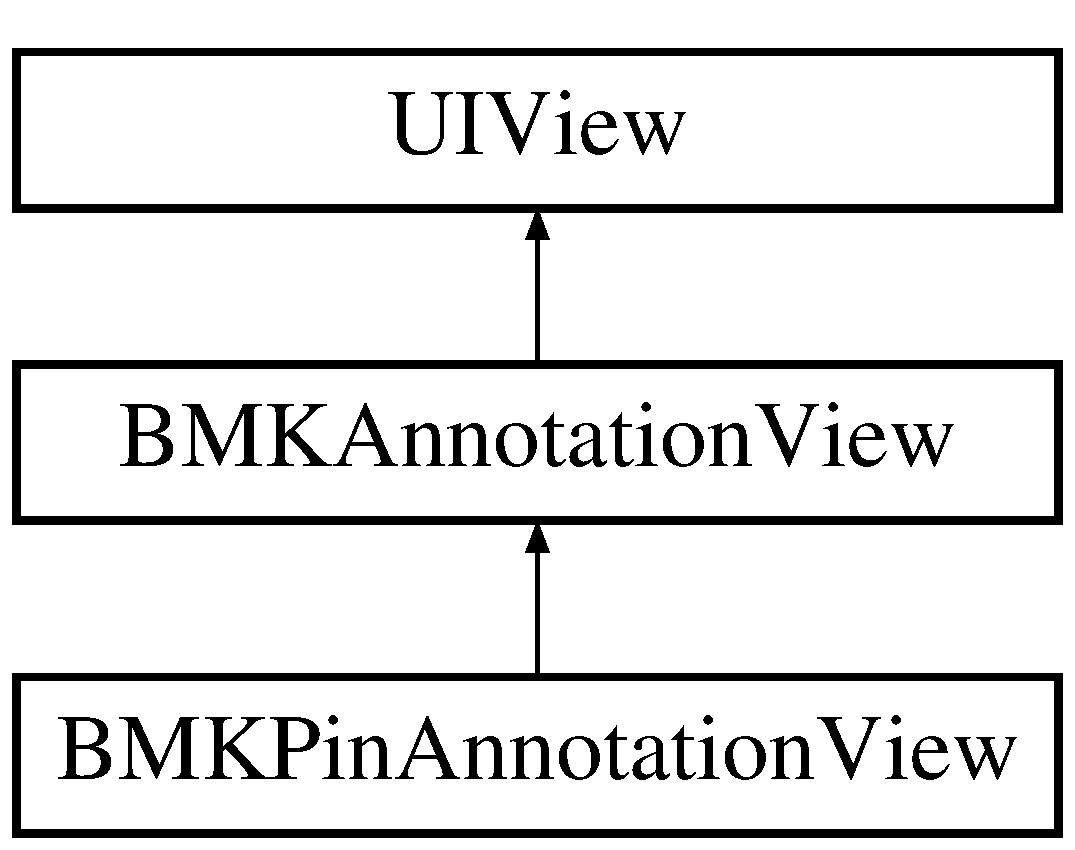
\includegraphics[height=3.000000cm]{interface_b_m_k_pin_annotation_view}
\end{center}
\end{figure}
\subsection*{Properties}
\begin{DoxyCompactItemize}
\item 
\hypertarget{interface_b_m_k_pin_annotation_view_a84f4c8db4dfa8d1d5a8ff6af8db7826d}{B\-M\-K\-Pin\-Annotation\-Color \hyperlink{interface_b_m_k_pin_annotation_view_a84f4c8db4dfa8d1d5a8ff6af8db7826d}{pin\-Color}}\label{interface_b_m_k_pin_annotation_view_a84f4c8db4dfa8d1d5a8ff6af8db7826d}

\begin{DoxyCompactList}\small\item\em 大头针的颜色,有\-B\-M\-K\-Pin\-Annotation\-Color\-Red, B\-M\-K\-Pin\-Annotation\-Color\-Green, B\-M\-K\-Pin\-Annotation\-Color\-Purple三种 \end{DoxyCompactList}\item 
\hypertarget{interface_b_m_k_pin_annotation_view_a0ea18aa3b2d71e06564bf11199d05625}{B\-O\-O\-L \hyperlink{interface_b_m_k_pin_annotation_view_a0ea18aa3b2d71e06564bf11199d05625}{animates\-Drop}}\label{interface_b_m_k_pin_annotation_view_a0ea18aa3b2d71e06564bf11199d05625}

\begin{DoxyCompactList}\small\item\em 动画效果 \end{DoxyCompactList}\end{DoxyCompactItemize}
\subsection*{附加继承成员}


\subsection{详细描述}
提供类似大头针效果的annotation view 

The documentation for this class was generated from the following file\-:\begin{DoxyCompactItemize}
\item 
B\-M\-K\-Pin\-Annotation\-View.\-h\end{DoxyCompactItemize}

\hypertarget{interface_b_m_k_plan_node}{\section{B\-M\-K\-Plan\-Node 类参考}
\label{interface_b_m_k_plan_node}\index{B\-M\-K\-Plan\-Node@{B\-M\-K\-Plan\-Node}}
}


线路节点信息  




{\ttfamily \#import $<$B\-M\-K\-Route\-Search\-Type.\-h$>$}

继承关系图 B\-M\-K\-Plan\-Node\-:\begin{figure}[H]
\begin{center}
\leavevmode
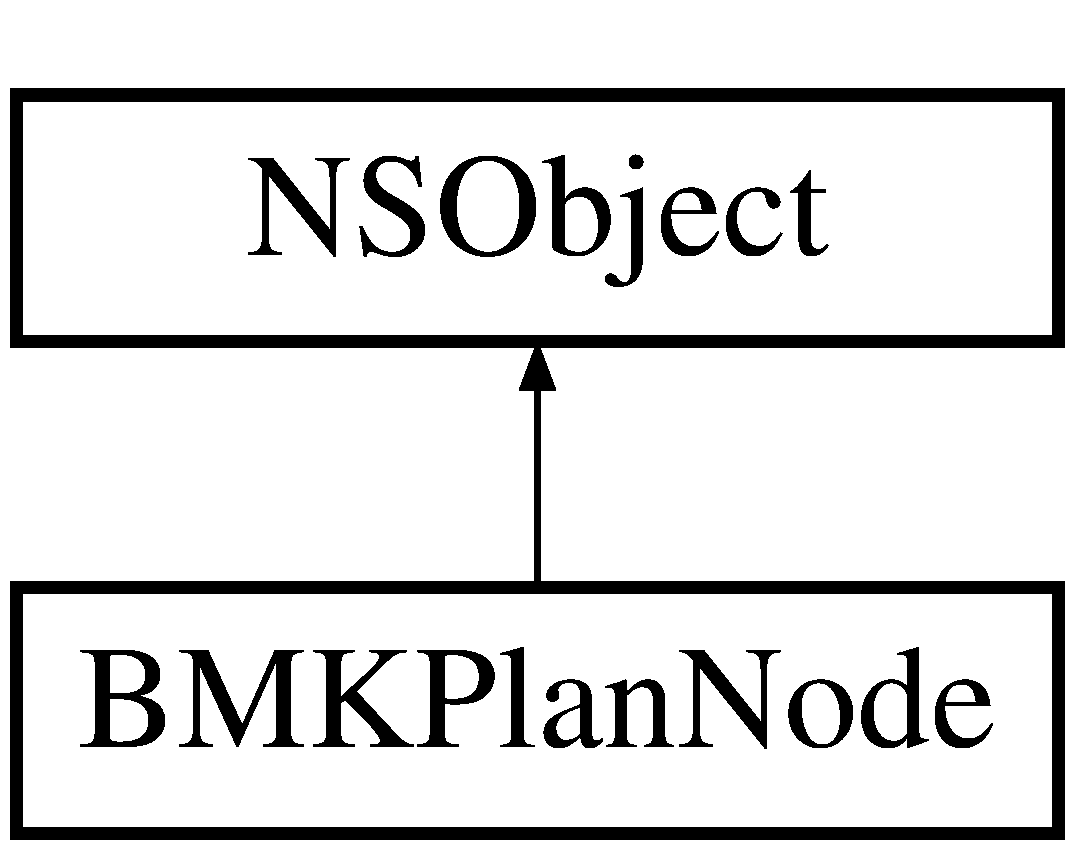
\includegraphics[height=2.000000cm]{interface_b_m_k_plan_node}
\end{center}
\end{figure}
\subsection*{保护成员变量}
\begin{DoxyCompactItemize}
\item 
\hypertarget{interface_b_m_k_plan_node_a1536db105328adee8a9e0c44804d8755}{N\-S\-String $\ast$ {\bfseries \-\_\-city\-Name}}\label{interface_b_m_k_plan_node_a1536db105328adee8a9e0c44804d8755}

\item 
\hypertarget{interface_b_m_k_plan_node_a6eeeeb61aa4389cea7e8ebb1d03a4d61}{N\-S\-String $\ast$ {\bfseries \-\_\-name}}\label{interface_b_m_k_plan_node_a6eeeeb61aa4389cea7e8ebb1d03a4d61}

\item 
\hypertarget{interface_b_m_k_plan_node_a503dbc9a4e2e07e81c3a701b64fcd3c3}{C\-L\-Location\-Coordinate2\-D {\bfseries \-\_\-pt}}\label{interface_b_m_k_plan_node_a503dbc9a4e2e07e81c3a701b64fcd3c3}

\end{DoxyCompactItemize}
\subsection*{Properties}
\begin{DoxyCompactItemize}
\item 
\hypertarget{interface_b_m_k_plan_node_ae6181a2e46740e8422a0b0820eedd0bb}{N\-S\-String $\ast$ \hyperlink{interface_b_m_k_plan_node_ae6181a2e46740e8422a0b0820eedd0bb}{city\-Name}}\label{interface_b_m_k_plan_node_ae6181a2e46740e8422a0b0820eedd0bb}

\begin{DoxyCompactList}\small\item\em 节点所在城市 \end{DoxyCompactList}\item 
\hypertarget{interface_b_m_k_plan_node_afe487565841e6361610e53d77af75f65}{N\-S\-String $\ast$ \hyperlink{interface_b_m_k_plan_node_afe487565841e6361610e53d77af75f65}{name}}\label{interface_b_m_k_plan_node_afe487565841e6361610e53d77af75f65}

\begin{DoxyCompactList}\small\item\em 节点名称 \end{DoxyCompactList}\item 
\hypertarget{interface_b_m_k_plan_node_a1fa1ff65e104926cc145168df5261136}{C\-L\-Location\-Coordinate2\-D \hyperlink{interface_b_m_k_plan_node_a1fa1ff65e104926cc145168df5261136}{pt}}\label{interface_b_m_k_plan_node_a1fa1ff65e104926cc145168df5261136}

\begin{DoxyCompactList}\small\item\em 节点坐标 \end{DoxyCompactList}\end{DoxyCompactItemize}


\subsection{详细描述}
线路节点信息 

The documentation for this class was generated from the following file\-:\begin{DoxyCompactItemize}
\item 
B\-M\-K\-Route\-Search\-Type.\-h\end{DoxyCompactItemize}

\hypertarget{interface_b_m_k_plan_result}{\section{B\-M\-K\-Plan\-Result 类参考}
\label{interface_b_m_k_plan_result}\index{B\-M\-K\-Plan\-Result@{B\-M\-K\-Plan\-Result}}
}


线路搜索结果类  




{\ttfamily \#import $<$B\-M\-K\-Route\-Search\-Type.\-h$>$}

继承关系图 B\-M\-K\-Plan\-Result\-:\begin{figure}[H]
\begin{center}
\leavevmode
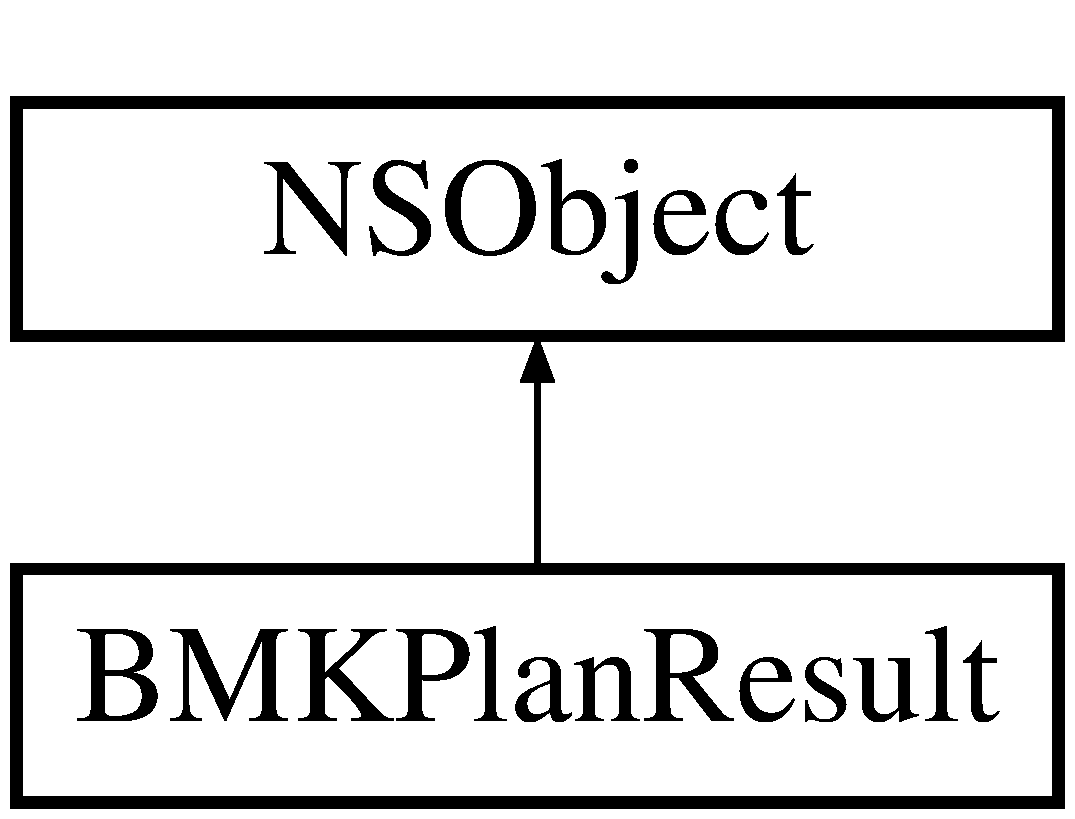
\includegraphics[height=2.000000cm]{interface_b_m_k_plan_result}
\end{center}
\end{figure}
\subsection*{保护成员变量}
\begin{DoxyCompactItemize}
\item 
\hypertarget{interface_b_m_k_plan_result_ad029efb37721d67673dee83e894a1660}{\hyperlink{interface_b_m_k_plan_node}{B\-M\-K\-Plan\-Node} $\ast$ {\bfseries \-\_\-end\-Node}}\label{interface_b_m_k_plan_result_ad029efb37721d67673dee83e894a1660}

\item 
\hypertarget{interface_b_m_k_plan_result_adb7a3aef50ec81cdb1fc5fa65dba5307}{N\-S\-Mutable\-Array $\ast$ {\bfseries \-\_\-way\-Nodes}}\label{interface_b_m_k_plan_result_adb7a3aef50ec81cdb1fc5fa65dba5307}

\item 
\hypertarget{interface_b_m_k_plan_result_a19418a00649c6af7e825887e3c394ac5}{N\-S\-Array $\ast$ {\bfseries \-\_\-plans}}\label{interface_b_m_k_plan_result_a19418a00649c6af7e825887e3c394ac5}

\item 
\hypertarget{interface_b_m_k_plan_result_aeb12dd0ff148a881e268bbf90dc8c4e5}{\hyperlink{interface_b_m_k_route_addr_result}{B\-M\-K\-Route\-Addr\-Result} $\ast$ {\bfseries \-\_\-route\-Addr\-Result}}\label{interface_b_m_k_plan_result_aeb12dd0ff148a881e268bbf90dc8c4e5}

\end{DoxyCompactItemize}
\subsection*{Properties}
\begin{DoxyCompactItemize}
\item 
\hypertarget{interface_b_m_k_plan_result_aa530b079304cbdb5a90d8d8e6eac86bc}{\hyperlink{interface_b_m_k_plan_node}{B\-M\-K\-Plan\-Node} $\ast$ {\bfseries \-\_\-start\-Node}}\label{interface_b_m_k_plan_result_aa530b079304cbdb5a90d8d8e6eac86bc}

\item 
\hypertarget{interface_b_m_k_plan_result_aa5e9caa3f38b8e60524848cd55440037}{\hyperlink{interface_b_m_k_plan_node}{B\-M\-K\-Plan\-Node} $\ast$ \hyperlink{interface_b_m_k_plan_result_aa5e9caa3f38b8e60524848cd55440037}{start\-Node}}\label{interface_b_m_k_plan_result_aa5e9caa3f38b8e60524848cd55440037}

\begin{DoxyCompactList}\small\item\em 线路起点 \end{DoxyCompactList}\item 
\hypertarget{interface_b_m_k_plan_result_a1fc0259719623cea6d79f7f5d1b03c78}{\hyperlink{interface_b_m_k_plan_node}{B\-M\-K\-Plan\-Node} $\ast$ \hyperlink{interface_b_m_k_plan_result_a1fc0259719623cea6d79f7f5d1b03c78}{end\-Node}}\label{interface_b_m_k_plan_result_a1fc0259719623cea6d79f7f5d1b03c78}

\begin{DoxyCompactList}\small\item\em 线路终点 \end{DoxyCompactList}\item 
\hypertarget{interface_b_m_k_plan_result_ac466beab9bb1db4ddb1375d588eee45a}{N\-S\-Array $\ast$ \hyperlink{interface_b_m_k_plan_result_ac466beab9bb1db4ddb1375d588eee45a}{way\-Nodes}}\label{interface_b_m_k_plan_result_ac466beab9bb1db4ddb1375d588eee45a}

\begin{DoxyCompactList}\small\item\em 路线途经点数组,包含的类型为(\-B\-M\-K\-Plan\-Node$\ast$) \end{DoxyCompactList}\item 
\hypertarget{interface_b_m_k_plan_result_a7200e21cfce75d49d825722fc42074e1}{N\-S\-Array $\ast$ \hyperlink{interface_b_m_k_plan_result_a7200e21cfce75d49d825722fc42074e1}{plans}}\label{interface_b_m_k_plan_result_a7200e21cfce75d49d825722fc42074e1}

\begin{DoxyCompactList}\small\item\em 方案数组 公交搜索返回\-B\-M\-K\-Transit\-Route\-Plan类型,驾车和步行返回\-B\-M\-K\-Route\-Plan类型 \end{DoxyCompactList}\item 
\hypertarget{interface_b_m_k_plan_result_a331a15353adf3028fa747083e95f6c77}{\hyperlink{interface_b_m_k_route_addr_result}{B\-M\-K\-Route\-Addr\-Result} $\ast$ \hyperlink{interface_b_m_k_plan_result_a331a15353adf3028fa747083e95f6c77}{route\-Addr\-Result}}\label{interface_b_m_k_plan_result_a331a15353adf3028fa747083e95f6c77}

\begin{DoxyCompactList}\small\item\em 返回起点或终点的地址信息结果 \end{DoxyCompactList}\end{DoxyCompactItemize}


\subsection{详细描述}
线路搜索结果类 

The documentation for this class was generated from the following file\-:\begin{DoxyCompactItemize}
\item 
B\-M\-K\-Route\-Search\-Type.\-h\end{DoxyCompactItemize}

\hypertarget{interface_b_m_k_poi_info}{\section{B\-M\-K\-Poi\-Info 类参考}
\label{interface_b_m_k_poi_info}\index{B\-M\-K\-Poi\-Info@{B\-M\-K\-Poi\-Info}}
}


P\-O\-I信息类  




{\ttfamily \#import $<$B\-M\-K\-Poi\-Search\-Type.\-h$>$}

继承关系图 B\-M\-K\-Poi\-Info\-:\begin{figure}[H]
\begin{center}
\leavevmode
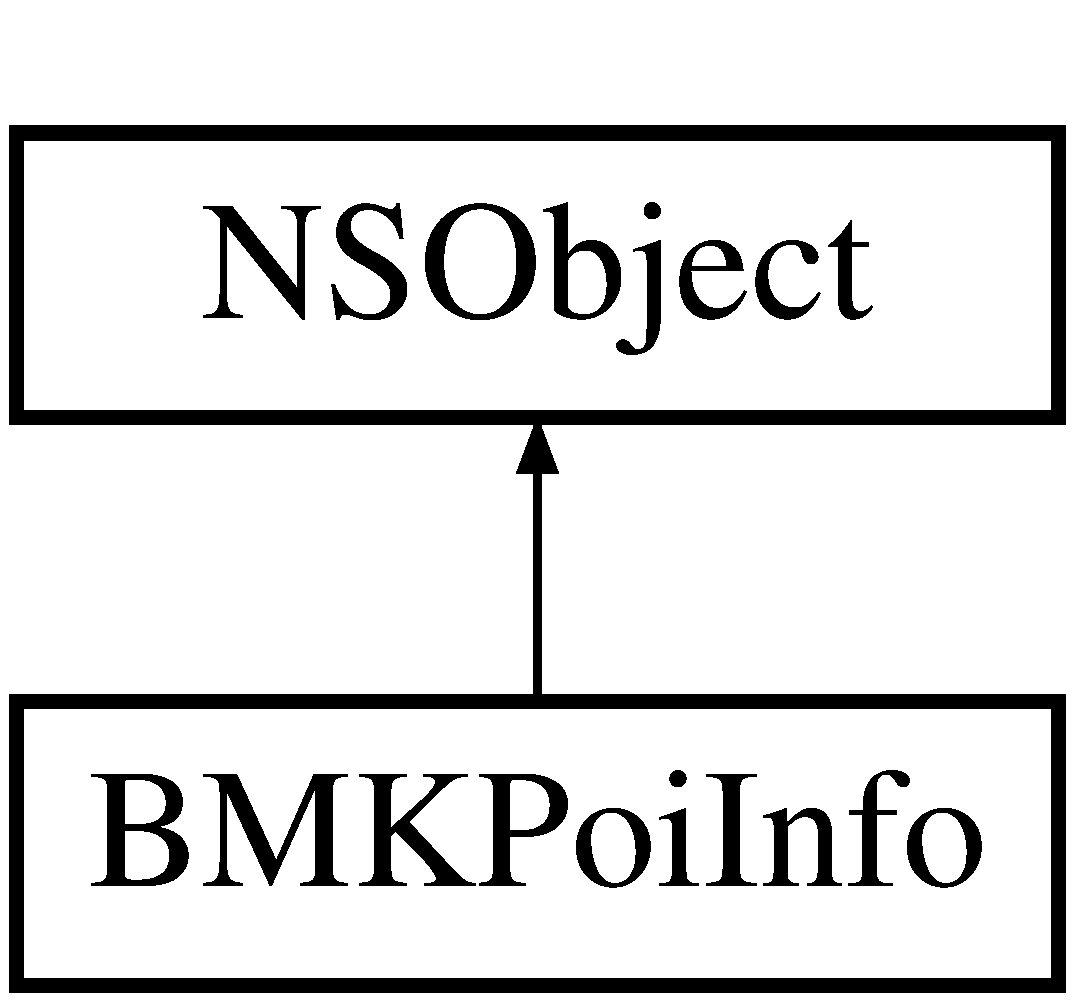
\includegraphics[height=2.000000cm]{interface_b_m_k_poi_info}
\end{center}
\end{figure}
\subsection*{保护成员变量}
\begin{DoxyCompactItemize}
\item 
\hypertarget{interface_b_m_k_poi_info_a5b4ebb41e4042d681b8f7b7720df84d1}{N\-S\-String $\ast$ {\bfseries \-\_\-uid}}\label{interface_b_m_k_poi_info_a5b4ebb41e4042d681b8f7b7720df84d1}

\item 
\hypertarget{interface_b_m_k_poi_info_a270dc7228aa502be45367e4d023ab238}{N\-S\-String $\ast$ \hyperlink{interface_b_m_k_poi_info_a270dc7228aa502be45367e4d023ab238}{\-\_\-address}}\label{interface_b_m_k_poi_info_a270dc7228aa502be45367e4d023ab238}

\begin{DoxyCompactList}\small\item\em P\-O\-I地址 \end{DoxyCompactList}\item 
\hypertarget{interface_b_m_k_poi_info_ad3239a4e452fe04daebee082134aa971}{N\-S\-String $\ast$ \hyperlink{interface_b_m_k_poi_info_ad3239a4e452fe04daebee082134aa971}{\-\_\-city}}\label{interface_b_m_k_poi_info_ad3239a4e452fe04daebee082134aa971}

\begin{DoxyCompactList}\small\item\em P\-O\-I所在城市 \end{DoxyCompactList}\item 
\hypertarget{interface_b_m_k_poi_info_a09b2b48d006e98069e1c11d020ee2eec}{N\-S\-String $\ast$ \hyperlink{interface_b_m_k_poi_info_a09b2b48d006e98069e1c11d020ee2eec}{\-\_\-phone}}\label{interface_b_m_k_poi_info_a09b2b48d006e98069e1c11d020ee2eec}

\begin{DoxyCompactList}\small\item\em P\-O\-I电话号码 \end{DoxyCompactList}\item 
\hypertarget{interface_b_m_k_poi_info_a4ef0d56b5d7ec9effd13c74fa2ecefe9}{N\-S\-String $\ast$ \hyperlink{interface_b_m_k_poi_info_a4ef0d56b5d7ec9effd13c74fa2ecefe9}{\-\_\-postcode}}\label{interface_b_m_k_poi_info_a4ef0d56b5d7ec9effd13c74fa2ecefe9}

\begin{DoxyCompactList}\small\item\em P\-O\-I邮编 \end{DoxyCompactList}\item 
\hypertarget{interface_b_m_k_poi_info_a5c00c72364b946887e29f42208cfa944}{int \hyperlink{interface_b_m_k_poi_info_a5c00c72364b946887e29f42208cfa944}{\-\_\-epoitype}}\label{interface_b_m_k_poi_info_a5c00c72364b946887e29f42208cfa944}

\begin{DoxyCompactList}\small\item\em P\-O\-I类型,0\-:普通点 1\-:公交站 2\-:公交线路 3\-:地铁站 4\-:地铁线路 \end{DoxyCompactList}\item 
\hypertarget{interface_b_m_k_poi_info_afe07d662e1b6c47a64cfa2bd8a70780b}{C\-L\-Location\-Coordinate2\-D \hyperlink{interface_b_m_k_poi_info_afe07d662e1b6c47a64cfa2bd8a70780b}{\-\_\-pt}}\label{interface_b_m_k_poi_info_afe07d662e1b6c47a64cfa2bd8a70780b}

\begin{DoxyCompactList}\small\item\em P\-O\-I坐标 \end{DoxyCompactList}\end{DoxyCompactItemize}
\subsection*{Properties}
\begin{DoxyCompactItemize}
\item 
\hypertarget{interface_b_m_k_poi_info_ab34c02df04b959fa0d2cfa141cd50c1e}{N\-S\-String $\ast$ \hyperlink{interface_b_m_k_poi_info_ab34c02df04b959fa0d2cfa141cd50c1e}{\-\_\-name}}\label{interface_b_m_k_poi_info_ab34c02df04b959fa0d2cfa141cd50c1e}

\begin{DoxyCompactList}\small\item\em P\-O\-I名称 \end{DoxyCompactList}\item 
\hypertarget{interface_b_m_k_poi_info_a58ff98eb46756c14f82a550974cf65b0}{N\-S\-String $\ast$ \hyperlink{interface_b_m_k_poi_info_a58ff98eb46756c14f82a550974cf65b0}{name}}\label{interface_b_m_k_poi_info_a58ff98eb46756c14f82a550974cf65b0}

\begin{DoxyCompactList}\small\item\em P\-O\-I名称 \end{DoxyCompactList}\item 
\hypertarget{interface_b_m_k_poi_info_a83caa34c026af8cc265d3b36c06f4c6b}{N\-S\-String $\ast$ \hyperlink{interface_b_m_k_poi_info_a83caa34c026af8cc265d3b36c06f4c6b}{uid}}\label{interface_b_m_k_poi_info_a83caa34c026af8cc265d3b36c06f4c6b}

\begin{DoxyCompactList}\small\item\em P\-O\-Iuid. \end{DoxyCompactList}\item 
\hypertarget{interface_b_m_k_poi_info_aa4bc4a2db1f2fa26fe77a8dad77fed21}{N\-S\-String $\ast$ \hyperlink{interface_b_m_k_poi_info_aa4bc4a2db1f2fa26fe77a8dad77fed21}{address}}\label{interface_b_m_k_poi_info_aa4bc4a2db1f2fa26fe77a8dad77fed21}

\begin{DoxyCompactList}\small\item\em P\-O\-I地址 \end{DoxyCompactList}\item 
\hypertarget{interface_b_m_k_poi_info_a4e4b4609a4fa81b653d642ed21d93e41}{N\-S\-String $\ast$ \hyperlink{interface_b_m_k_poi_info_a4e4b4609a4fa81b653d642ed21d93e41}{city}}\label{interface_b_m_k_poi_info_a4e4b4609a4fa81b653d642ed21d93e41}

\begin{DoxyCompactList}\small\item\em P\-O\-I所在城市 \end{DoxyCompactList}\item 
\hypertarget{interface_b_m_k_poi_info_a12400456544f0542682c09b8e443553d}{N\-S\-String $\ast$ \hyperlink{interface_b_m_k_poi_info_a12400456544f0542682c09b8e443553d}{phone}}\label{interface_b_m_k_poi_info_a12400456544f0542682c09b8e443553d}

\begin{DoxyCompactList}\small\item\em P\-O\-I电话号码 \end{DoxyCompactList}\item 
\hypertarget{interface_b_m_k_poi_info_a696c50cfef411e4c8aa4a53693c26dc5}{N\-S\-String $\ast$ \hyperlink{interface_b_m_k_poi_info_a696c50cfef411e4c8aa4a53693c26dc5}{postcode}}\label{interface_b_m_k_poi_info_a696c50cfef411e4c8aa4a53693c26dc5}

\begin{DoxyCompactList}\small\item\em P\-O\-I邮编 \end{DoxyCompactList}\item 
\hypertarget{interface_b_m_k_poi_info_ada3ccb40708069fe5d82414af8de1ab5}{int \hyperlink{interface_b_m_k_poi_info_ada3ccb40708069fe5d82414af8de1ab5}{epoitype}}\label{interface_b_m_k_poi_info_ada3ccb40708069fe5d82414af8de1ab5}

\begin{DoxyCompactList}\small\item\em P\-O\-I类型,0\-:普通点 1\-:公交站 2\-:公交线路 3\-:地铁站 4\-:地铁线路 \end{DoxyCompactList}\item 
\hypertarget{interface_b_m_k_poi_info_a6ace0b9f9462c1695317654d92c3795a}{C\-L\-Location\-Coordinate2\-D \hyperlink{interface_b_m_k_poi_info_a6ace0b9f9462c1695317654d92c3795a}{pt}}\label{interface_b_m_k_poi_info_a6ace0b9f9462c1695317654d92c3795a}

\begin{DoxyCompactList}\small\item\em P\-O\-I坐标 \end{DoxyCompactList}\end{DoxyCompactItemize}


\subsection{详细描述}
P\-O\-I信息类 

The documentation for this class was generated from the following file\-:\begin{DoxyCompactItemize}
\item 
B\-M\-K\-Poi\-Search\-Type.\-h\end{DoxyCompactItemize}

\hypertarget{interface_b_m_k_point_annotation}{\section{B\-M\-K\-Point\-Annotation 类参考}
\label{interface_b_m_k_point_annotation}\index{B\-M\-K\-Point\-Annotation@{B\-M\-K\-Point\-Annotation}}
}


表示一个点的annotation  




{\ttfamily \#import $<$B\-M\-K\-Point\-Annotation.\-h$>$}

继承关系图 B\-M\-K\-Point\-Annotation\-:\begin{figure}[H]
\begin{center}
\leavevmode
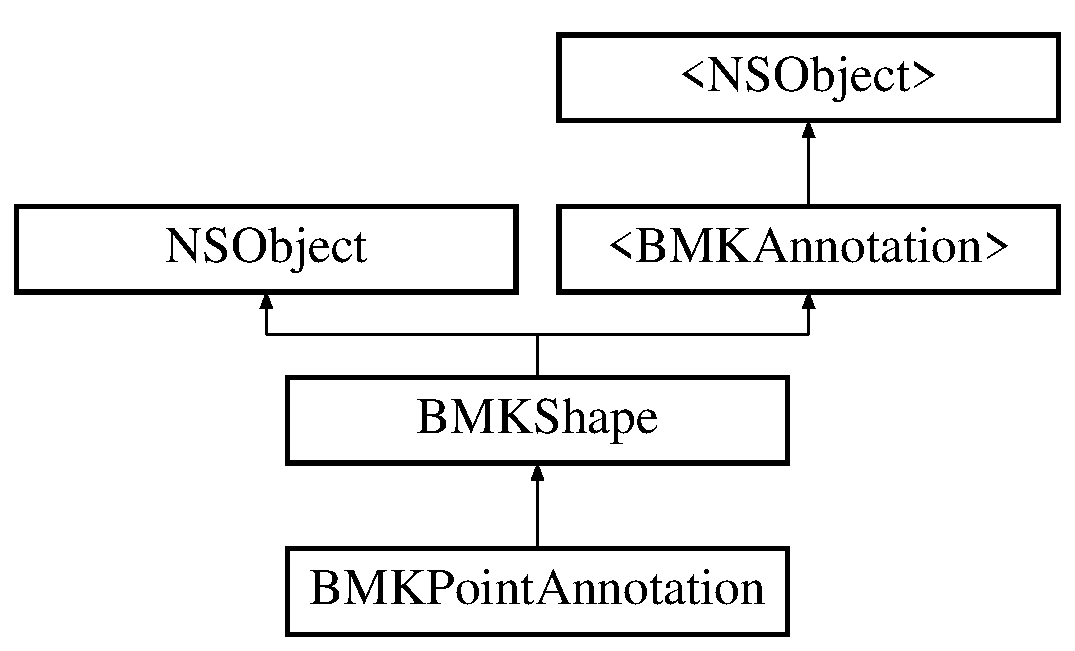
\includegraphics[height=4.000000cm]{interface_b_m_k_point_annotation}
\end{center}
\end{figure}
\subsection*{保护成员变量}
\begin{DoxyCompactItemize}
\item 
\hypertarget{interface_b_m_k_point_annotation_affd501bbf19fb485a6bd7e0e49c9a144}{package C\-L\-Location\-Coordinate2\-D {\bfseries \-\_\-coordinate}}\label{interface_b_m_k_point_annotation_affd501bbf19fb485a6bd7e0e49c9a144}

\end{DoxyCompactItemize}
\subsection*{Properties}
\begin{DoxyCompactItemize}
\item 
\hypertarget{interface_b_m_k_point_annotation_a4434c998ea13f0c029eb944312611091}{C\-L\-Location\-Coordinate2\-D \hyperlink{interface_b_m_k_point_annotation_a4434c998ea13f0c029eb944312611091}{coordinate}}\label{interface_b_m_k_point_annotation_a4434c998ea13f0c029eb944312611091}

\begin{DoxyCompactList}\small\item\em 该点的坐标 \end{DoxyCompactList}\end{DoxyCompactItemize}
\subsection*{附加继承成员}


\subsection{详细描述}
表示一个点的annotation 

The documentation for this class was generated from the following file\-:\begin{DoxyCompactItemize}
\item 
B\-M\-K\-Point\-Annotation.\-h\end{DoxyCompactItemize}

\hypertarget{interface_b_m_k_poi_result}{\section{B\-M\-K\-Poi\-Result 类参考}
\label{interface_b_m_k_poi_result}\index{B\-M\-K\-Poi\-Result@{B\-M\-K\-Poi\-Result}}
}


P\-O\-I搜索结果类  




{\ttfamily \#import $<$B\-M\-K\-Poi\-Search\-Type.\-h$>$}

继承关系图 B\-M\-K\-Poi\-Result\-:\begin{figure}[H]
\begin{center}
\leavevmode
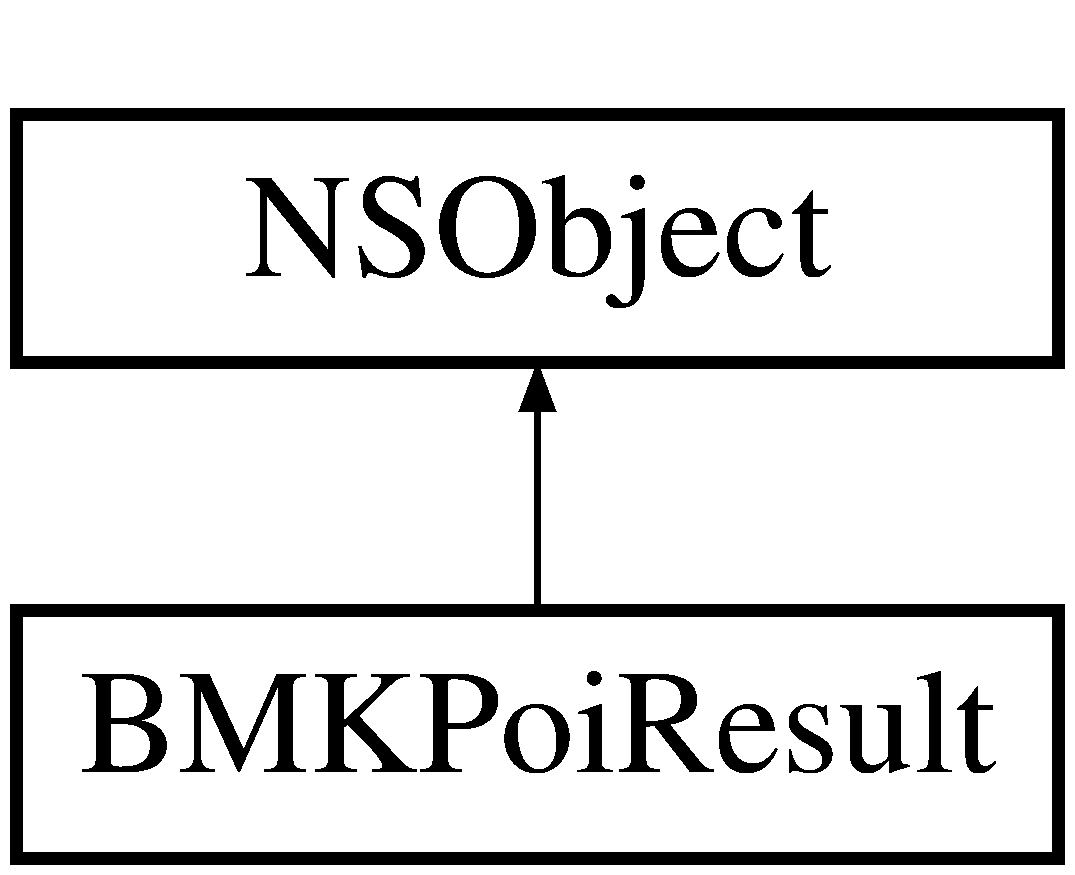
\includegraphics[height=2.000000cm]{interface_b_m_k_poi_result}
\end{center}
\end{figure}
\subsection*{保护成员变量}
\begin{DoxyCompactItemize}
\item 
\hypertarget{interface_b_m_k_poi_result_a734c9424931aaa457069c0179c22d307}{int \hyperlink{interface_b_m_k_poi_result_a734c9424931aaa457069c0179c22d307}{\-\_\-curr\-Poi\-Num}}\label{interface_b_m_k_poi_result_a734c9424931aaa457069c0179c22d307}

\begin{DoxyCompactList}\small\item\em 当前页的\-P\-O\-I结果数 \end{DoxyCompactList}\item 
\hypertarget{interface_b_m_k_poi_result_a5831f7fc7e978e04e58fe9f3a1da0fd7}{int \hyperlink{interface_b_m_k_poi_result_a5831f7fc7e978e04e58fe9f3a1da0fd7}{\-\_\-page\-Num}}\label{interface_b_m_k_poi_result_a5831f7fc7e978e04e58fe9f3a1da0fd7}

\begin{DoxyCompactList}\small\item\em 本次\-P\-O\-I搜索的总页数 \end{DoxyCompactList}\item 
\hypertarget{interface_b_m_k_poi_result_a0b75833625c93cd9c4d4fc225324cee1}{int \hyperlink{interface_b_m_k_poi_result_a0b75833625c93cd9c4d4fc225324cee1}{\-\_\-page\-Index}}\label{interface_b_m_k_poi_result_a0b75833625c93cd9c4d4fc225324cee1}

\begin{DoxyCompactList}\small\item\em 当前页的索引 \end{DoxyCompactList}\item 
\hypertarget{interface_b_m_k_poi_result_a25244becb10392bdb2d9d781d357208d}{N\-S\-Array $\ast$ \hyperlink{interface_b_m_k_poi_result_a25244becb10392bdb2d9d781d357208d}{\-\_\-poi\-Info\-List}}\label{interface_b_m_k_poi_result_a25244becb10392bdb2d9d781d357208d}

\begin{DoxyCompactList}\small\item\em P\-O\-I列表,成员是\-B\-M\-K\-Poi\-Info. \end{DoxyCompactList}\item 
\hypertarget{interface_b_m_k_poi_result_acf4e2c4c0040c79368d2da36bfd7c092}{N\-S\-Array $\ast$ \hyperlink{interface_b_m_k_poi_result_acf4e2c4c0040c79368d2da36bfd7c092}{\-\_\-city\-List}}\label{interface_b_m_k_poi_result_acf4e2c4c0040c79368d2da36bfd7c092}

\begin{DoxyCompactList}\small\item\em 城市列表,成员是\-B\-M\-K\-City\-List\-Info \end{DoxyCompactList}\end{DoxyCompactItemize}
\subsection*{Properties}
\begin{DoxyCompactItemize}
\item 
\hypertarget{interface_b_m_k_poi_result_a4a48255798b55903c7ffc1f4a5fd20aa}{int \hyperlink{interface_b_m_k_poi_result_a4a48255798b55903c7ffc1f4a5fd20aa}{\-\_\-total\-Poi\-Num}}\label{interface_b_m_k_poi_result_a4a48255798b55903c7ffc1f4a5fd20aa}

\begin{DoxyCompactList}\small\item\em 本次\-P\-O\-I搜索的总结果数 \end{DoxyCompactList}\item 
\hypertarget{interface_b_m_k_poi_result_aa4c147655cc6c787a10794c91cf6d525}{int \hyperlink{interface_b_m_k_poi_result_aa4c147655cc6c787a10794c91cf6d525}{total\-Poi\-Num}}\label{interface_b_m_k_poi_result_aa4c147655cc6c787a10794c91cf6d525}

\begin{DoxyCompactList}\small\item\em 本次\-P\-O\-I搜索的总结果数 \end{DoxyCompactList}\item 
\hypertarget{interface_b_m_k_poi_result_aafa2dcb8b8faf851b011ac268a37dc8e}{int \hyperlink{interface_b_m_k_poi_result_aafa2dcb8b8faf851b011ac268a37dc8e}{curr\-Poi\-Num}}\label{interface_b_m_k_poi_result_aafa2dcb8b8faf851b011ac268a37dc8e}

\begin{DoxyCompactList}\small\item\em 当前页的\-P\-O\-I结果数 \end{DoxyCompactList}\item 
\hypertarget{interface_b_m_k_poi_result_aa5985334edff4ec10dacf4bcdbf7c5f8}{int \hyperlink{interface_b_m_k_poi_result_aa5985334edff4ec10dacf4bcdbf7c5f8}{page\-Num}}\label{interface_b_m_k_poi_result_aa5985334edff4ec10dacf4bcdbf7c5f8}

\begin{DoxyCompactList}\small\item\em 本次\-P\-O\-I搜索的总页数 \end{DoxyCompactList}\item 
\hypertarget{interface_b_m_k_poi_result_a7f4e48d20ae32404d0113f4224e8bad3}{int \hyperlink{interface_b_m_k_poi_result_a7f4e48d20ae32404d0113f4224e8bad3}{page\-Index}}\label{interface_b_m_k_poi_result_a7f4e48d20ae32404d0113f4224e8bad3}

\begin{DoxyCompactList}\small\item\em 当前页的索引 \end{DoxyCompactList}\item 
\hypertarget{interface_b_m_k_poi_result_a4f5475068a92bab6e67f47654e8c6256}{N\-S\-Array $\ast$ \hyperlink{interface_b_m_k_poi_result_a4f5475068a92bab6e67f47654e8c6256}{poi\-Info\-List}}\label{interface_b_m_k_poi_result_a4f5475068a92bab6e67f47654e8c6256}

\begin{DoxyCompactList}\small\item\em P\-O\-I列表,成员是\-B\-M\-K\-Poi\-Info. \end{DoxyCompactList}\item 
\hypertarget{interface_b_m_k_poi_result_a8315d8ec2e803b8dd3af74b197b4aa80}{N\-S\-Array $\ast$ \hyperlink{interface_b_m_k_poi_result_a8315d8ec2e803b8dd3af74b197b4aa80}{city\-List}}\label{interface_b_m_k_poi_result_a8315d8ec2e803b8dd3af74b197b4aa80}

\begin{DoxyCompactList}\small\item\em 城市列表,成员是\-B\-M\-K\-City\-List\-Info \end{DoxyCompactList}\end{DoxyCompactItemize}


\subsection{详细描述}
P\-O\-I搜索结果类 

The documentation for this class was generated from the following file\-:\begin{DoxyCompactItemize}
\item 
B\-M\-K\-Poi\-Search\-Type.\-h\end{DoxyCompactItemize}

\hypertarget{interface_b_m_k_polygon}{\section{B\-M\-K\-Polygon 类参考}
\label{interface_b_m_k_polygon}\index{B\-M\-K\-Polygon@{B\-M\-K\-Polygon}}
}


此类用于定义一个多边形区域  




{\ttfamily \#import $<$B\-M\-K\-Polygon.\-h$>$}

继承关系图 B\-M\-K\-Polygon\-:\begin{figure}[H]
\begin{center}
\leavevmode
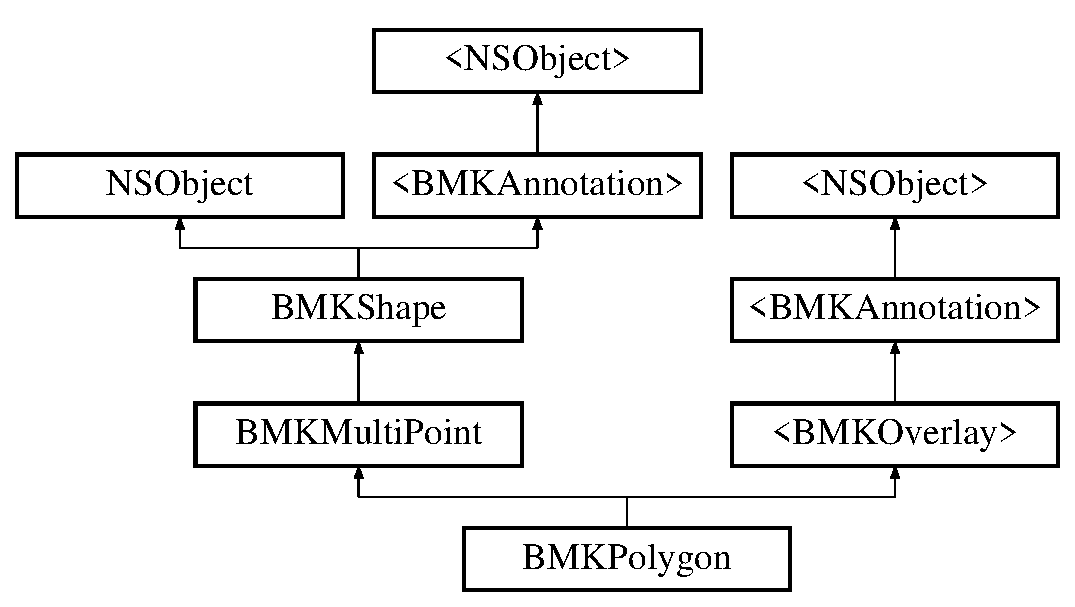
\includegraphics[height=5.000000cm]{interface_b_m_k_polygon}
\end{center}
\end{figure}
\subsection*{类方法}
\begin{DoxyCompactItemize}
\item 
(\hyperlink{interface_b_m_k_polygon}{B\-M\-K\-Polygon} $\ast$) + \hyperlink{interface_b_m_k_polygon_a74b92a200709fb4c6718b26ebdfcc50a}{polygon\-With\-Points\-:count\-:}
\item 
(\hyperlink{interface_b_m_k_polygon}{B\-M\-K\-Polygon} $\ast$) + \hyperlink{interface_b_m_k_polygon_aa4d03b7361ffc6b93721d456e62b14b0}{polygon\-With\-Points\-:count\-:interior\-Polygons\-:}
\item 
(\hyperlink{interface_b_m_k_polygon}{B\-M\-K\-Polygon} $\ast$) + \hyperlink{interface_b_m_k_polygon_aa3de0deeba040969c9211b64c59831f2}{polygon\-With\-Coordinates\-:count\-:}
\item 
(\hyperlink{interface_b_m_k_polygon}{B\-M\-K\-Polygon} $\ast$) + \hyperlink{interface_b_m_k_polygon_a298e0f0578320ab5419a9e150ffc0714}{polygon\-With\-Coordinates\-:count\-:interior\-Polygons\-:}
\end{DoxyCompactItemize}
\subsection*{保护成员变量}
\begin{DoxyCompactItemize}
\item 
\hypertarget{interface_b_m_k_polygon_ab6ba9bddb4458202dc547dd3a7d2f880}{package C\-L\-Location\-Coordinate2\-D {\bfseries \-\_\-centroid}}\label{interface_b_m_k_polygon_ab6ba9bddb4458202dc547dd3a7d2f880}

\item 
\hypertarget{interface_b_m_k_polygon_a2f794615e03edb6c089d892ee93c7f98}{N\-S\-Array $\ast$ {\bfseries \-\_\-interior\-Polygons}}\label{interface_b_m_k_polygon_a2f794615e03edb6c089d892ee93c7f98}

\item 
\hypertarget{interface_b_m_k_polygon_ac422f2bfe27b80c7b34a8f4d4c8bb4bb}{B\-O\-O\-L {\bfseries \-\_\-is\-Definitely\-Convex}}\label{interface_b_m_k_polygon_ac422f2bfe27b80c7b34a8f4d4c8bb4bb}

\end{DoxyCompactItemize}
\subsection*{Properties}
\begin{DoxyCompactItemize}
\item 
\hypertarget{interface_b_m_k_polygon_a7ff1fd88f27c07dbd6a2243178d7f8c4}{N\-S\-Array $\ast$ \hyperlink{interface_b_m_k_polygon_a7ff1fd88f27c07dbd6a2243178d7f8c4}{interior\-Polygons}}\label{interface_b_m_k_polygon_a7ff1fd88f27c07dbd6a2243178d7f8c4}

\begin{DoxyCompactList}\small\item\em 内部多边形数组 \end{DoxyCompactList}\end{DoxyCompactItemize}
\subsection*{附加继承成员}


\subsection{详细描述}
此类用于定义一个多边形区域 

\subsection{方法文档}
\hypertarget{interface_b_m_k_polygon_aa3de0deeba040969c9211b64c59831f2}{\index{B\-M\-K\-Polygon@{B\-M\-K\-Polygon}!polygon\-With\-Coordinates\-:count\-:@{polygon\-With\-Coordinates\-:count\-:}}
\index{polygon\-With\-Coordinates\-:count\-:@{polygon\-With\-Coordinates\-:count\-:}!BMKPolygon@{B\-M\-K\-Polygon}}
\subsubsection[{polygon\-With\-Coordinates\-:count\-:}]{\setlength{\rightskip}{0pt plus 5cm}+ ({\bf B\-M\-K\-Polygon} $\ast$) polygon\-With\-Coordinates\-: 
\begin{DoxyParamCaption}
\item[{(C\-L\-Location\-Coordinate2\-D $\ast$)}]{coords}
\item[{count:(N\-S\-U\-Integer)}]{count}
\end{DoxyParamCaption}
}}\label{interface_b_m_k_polygon_aa3de0deeba040969c9211b64c59831f2}
根据多个点生成多边形 
\begin{DoxyParams}{参数}
{\em coords} & 经纬度坐标点数组,这些点将被拷贝到生成的多边形对象中 \\
\hline
{\em count} & 点的个数 \\
\hline
\end{DoxyParams}
\begin{DoxyReturn}{返回}
新生成的多边形对象 
\end{DoxyReturn}
\hypertarget{interface_b_m_k_polygon_a298e0f0578320ab5419a9e150ffc0714}{\index{B\-M\-K\-Polygon@{B\-M\-K\-Polygon}!polygon\-With\-Coordinates\-:count\-:interior\-Polygons\-:@{polygon\-With\-Coordinates\-:count\-:interior\-Polygons\-:}}
\index{polygon\-With\-Coordinates\-:count\-:interior\-Polygons\-:@{polygon\-With\-Coordinates\-:count\-:interior\-Polygons\-:}!BMKPolygon@{B\-M\-K\-Polygon}}
\subsubsection[{polygon\-With\-Coordinates\-:count\-:interior\-Polygons\-:}]{\setlength{\rightskip}{0pt plus 5cm}+ ({\bf B\-M\-K\-Polygon} $\ast$) polygon\-With\-Coordinates\-: 
\begin{DoxyParamCaption}
\item[{(C\-L\-Location\-Coordinate2\-D $\ast$)}]{coords}
\item[{count:(N\-S\-U\-Integer)}]{count}
\item[{interiorPolygons:(N\-S\-Array $\ast$)}]{interior\-Polygons}
\end{DoxyParamCaption}
}}\label{interface_b_m_k_polygon_a298e0f0578320ab5419a9e150ffc0714}
根据多个点及指定的内部镂空多边形数组生成新的多边形对象 
\begin{DoxyParams}{参数}
{\em coords} & 经纬度坐标点数组,这些点将被拷贝到生成的多边形对象中 \\
\hline
{\em count} & 点的个数 \\
\hline
{\em interior\-Polygons} & 指定的内部镂空多边形数组 \\
\hline
\end{DoxyParams}
\begin{DoxyReturn}{返回}
新生成的多边形对象 
\end{DoxyReturn}
\hypertarget{interface_b_m_k_polygon_a74b92a200709fb4c6718b26ebdfcc50a}{\index{B\-M\-K\-Polygon@{B\-M\-K\-Polygon}!polygon\-With\-Points\-:count\-:@{polygon\-With\-Points\-:count\-:}}
\index{polygon\-With\-Points\-:count\-:@{polygon\-With\-Points\-:count\-:}!BMKPolygon@{B\-M\-K\-Polygon}}
\subsubsection[{polygon\-With\-Points\-:count\-:}]{\setlength{\rightskip}{0pt plus 5cm}+ ({\bf B\-M\-K\-Polygon} $\ast$) polygon\-With\-Points\-: 
\begin{DoxyParamCaption}
\item[{({\bf B\-M\-K\-Map\-Point} $\ast$)}]{points}
\item[{count:(N\-S\-U\-Integer)}]{count}
\end{DoxyParamCaption}
}}\label{interface_b_m_k_polygon_a74b92a200709fb4c6718b26ebdfcc50a}
根据多个点生成多边形 
\begin{DoxyParams}{参数}
{\em points} & 直角坐标点数组,这些点将被拷贝到生成的多边形对象中 \\
\hline
{\em count} & 点的个数 \\
\hline
\end{DoxyParams}
\begin{DoxyReturn}{返回}
新生成的多边形对象 
\end{DoxyReturn}
\hypertarget{interface_b_m_k_polygon_aa4d03b7361ffc6b93721d456e62b14b0}{\index{B\-M\-K\-Polygon@{B\-M\-K\-Polygon}!polygon\-With\-Points\-:count\-:interior\-Polygons\-:@{polygon\-With\-Points\-:count\-:interior\-Polygons\-:}}
\index{polygon\-With\-Points\-:count\-:interior\-Polygons\-:@{polygon\-With\-Points\-:count\-:interior\-Polygons\-:}!BMKPolygon@{B\-M\-K\-Polygon}}
\subsubsection[{polygon\-With\-Points\-:count\-:interior\-Polygons\-:}]{\setlength{\rightskip}{0pt plus 5cm}+ ({\bf B\-M\-K\-Polygon} $\ast$) polygon\-With\-Points\-: 
\begin{DoxyParamCaption}
\item[{({\bf B\-M\-K\-Map\-Point} $\ast$)}]{points}
\item[{count:(N\-S\-U\-Integer)}]{count}
\item[{interiorPolygons:(N\-S\-Array $\ast$)}]{interior\-Polygons}
\end{DoxyParamCaption}
}}\label{interface_b_m_k_polygon_aa4d03b7361ffc6b93721d456e62b14b0}
根据多个点及指定的内部镂空多边形数组生成新的多边形对象 
\begin{DoxyParams}{参数}
{\em points} & 直角坐标点数组,这些点将被拷贝到生成的多边形对象中 \\
\hline
{\em count} & 点的个数 \\
\hline
{\em interior\-Polygons} & 指定的内部镂空多边形数组 \\
\hline
\end{DoxyParams}
\begin{DoxyReturn}{返回}
新生成的多边形对象 
\end{DoxyReturn}


The documentation for this class was generated from the following file\-:\begin{DoxyCompactItemize}
\item 
B\-M\-K\-Polygon.\-h\end{DoxyCompactItemize}

\hypertarget{interface_b_m_k_polygon_view}{\section{B\-M\-K\-Polygon\-View 类参考}
\label{interface_b_m_k_polygon_view}\index{B\-M\-K\-Polygon\-View@{B\-M\-K\-Polygon\-View}}
}


此类用于定义一个多边形\-View  




{\ttfamily \#import $<$B\-M\-K\-Polygon\-View.\-h$>$}

继承关系图 B\-M\-K\-Polygon\-View\-:\begin{figure}[H]
\begin{center}
\leavevmode
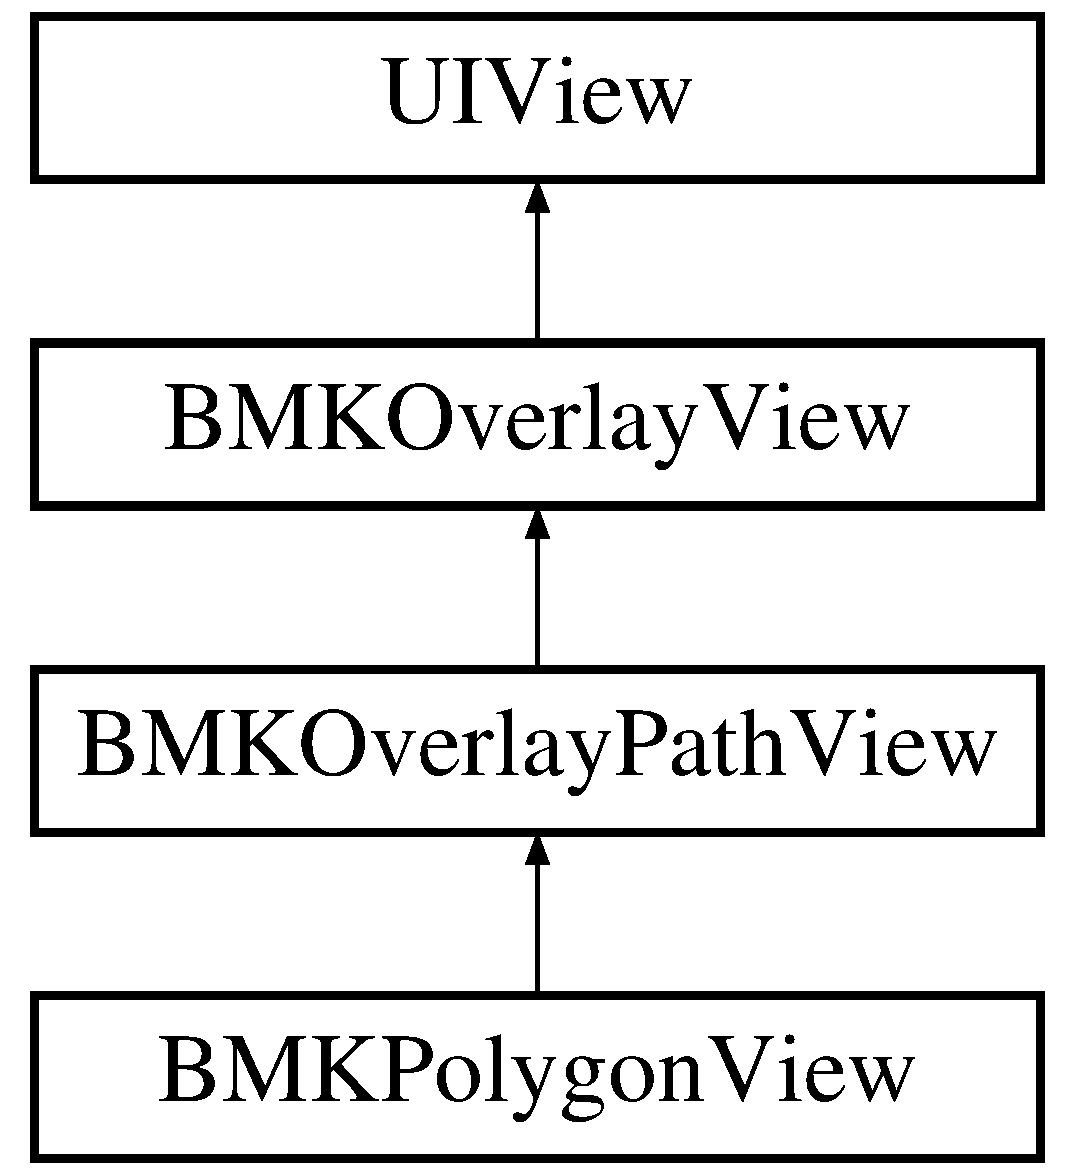
\includegraphics[height=4.000000cm]{interface_b_m_k_polygon_view}
\end{center}
\end{figure}
\subsection*{实例方法}
\begin{DoxyCompactItemize}
\item 
(id) -\/ \hyperlink{interface_b_m_k_polygon_view_a447c40c6fd5c04668d7b9da823a5af26}{init\-With\-Polygon\-:}
\end{DoxyCompactItemize}
\subsection*{Properties}
\begin{DoxyCompactItemize}
\item 
\hypertarget{interface_b_m_k_polygon_view_afcb56ec12abe7a03236d732f63f555bd}{\hyperlink{interface_b_m_k_polygon}{B\-M\-K\-Polygon} $\ast$ \hyperlink{interface_b_m_k_polygon_view_afcb56ec12abe7a03236d732f63f555bd}{polygon}}\label{interface_b_m_k_polygon_view_afcb56ec12abe7a03236d732f63f555bd}

\begin{DoxyCompactList}\small\item\em 该\-View对应的多边形数据 \end{DoxyCompactList}\end{DoxyCompactItemize}
\subsection*{附加继承成员}


\subsection{详细描述}
此类用于定义一个多边形\-View 

\subsection{方法文档}
\hypertarget{interface_b_m_k_polygon_view_a447c40c6fd5c04668d7b9da823a5af26}{\index{B\-M\-K\-Polygon\-View@{B\-M\-K\-Polygon\-View}!init\-With\-Polygon\-:@{init\-With\-Polygon\-:}}
\index{init\-With\-Polygon\-:@{init\-With\-Polygon\-:}!BMKPolygonView@{B\-M\-K\-Polygon\-View}}
\subsubsection[{init\-With\-Polygon\-:}]{\setlength{\rightskip}{0pt plus 5cm}-\/ (id) init\-With\-Polygon\-: 
\begin{DoxyParamCaption}
\item[{({\bf B\-M\-K\-Polygon} $\ast$)}]{polygon}
\end{DoxyParamCaption}
}}\label{interface_b_m_k_polygon_view_a447c40c6fd5c04668d7b9da823a5af26}
根据指定的多边形生成一个多边形\-View 
\begin{DoxyParams}{参数}
{\em polygon} & 指定的多边形数据对象 \\
\hline
\end{DoxyParams}
\begin{DoxyReturn}{返回}
新生成的多边形\-View 
\end{DoxyReturn}


The documentation for this class was generated from the following file\-:\begin{DoxyCompactItemize}
\item 
B\-M\-K\-Polygon\-View.\-h\end{DoxyCompactItemize}

\hypertarget{interface_b_m_k_polyline}{\section{B\-M\-K\-Polyline 类参考}
\label{interface_b_m_k_polyline}\index{B\-M\-K\-Polyline@{B\-M\-K\-Polyline}}
}


此类用于定义一段折线  




{\ttfamily \#import $<$B\-M\-K\-Polyline.\-h$>$}

继承关系图 B\-M\-K\-Polyline\-:\begin{figure}[H]
\begin{center}
\leavevmode
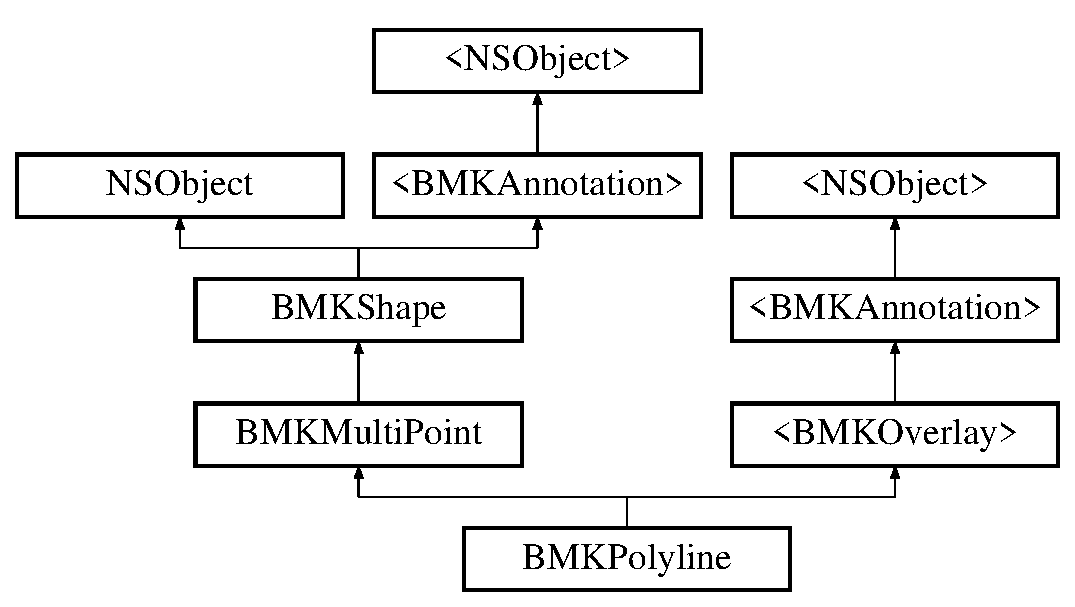
\includegraphics[height=5.000000cm]{interface_b_m_k_polyline}
\end{center}
\end{figure}
\subsection*{类方法}
\begin{DoxyCompactItemize}
\item 
(\hyperlink{interface_b_m_k_polyline}{B\-M\-K\-Polyline} $\ast$) + \hyperlink{interface_b_m_k_polyline_aa4f399b9bcc1c33b871b3d8152842eac}{polyline\-With\-Points\-:count\-:}
\item 
(\hyperlink{interface_b_m_k_polyline}{B\-M\-K\-Polyline} $\ast$) + \hyperlink{interface_b_m_k_polyline_af43f8ff39d6a8c56f28f3294f9c41681}{polyline\-With\-Coordinates\-:count\-:}
\end{DoxyCompactItemize}
\subsection*{附加继承成员}


\subsection{详细描述}
此类用于定义一段折线 

\subsection{方法文档}
\hypertarget{interface_b_m_k_polyline_af43f8ff39d6a8c56f28f3294f9c41681}{\index{B\-M\-K\-Polyline@{B\-M\-K\-Polyline}!polyline\-With\-Coordinates\-:count\-:@{polyline\-With\-Coordinates\-:count\-:}}
\index{polyline\-With\-Coordinates\-:count\-:@{polyline\-With\-Coordinates\-:count\-:}!BMKPolyline@{B\-M\-K\-Polyline}}
\subsubsection[{polyline\-With\-Coordinates\-:count\-:}]{\setlength{\rightskip}{0pt plus 5cm}+ ({\bf B\-M\-K\-Polyline} $\ast$) polyline\-With\-Coordinates\-: 
\begin{DoxyParamCaption}
\item[{(C\-L\-Location\-Coordinate2\-D $\ast$)}]{coords}
\item[{count:(N\-S\-U\-Integer)}]{count}
\end{DoxyParamCaption}
}}\label{interface_b_m_k_polyline_af43f8ff39d6a8c56f28f3294f9c41681}
根据指定坐标点生成一段折线 
\begin{DoxyParams}{参数}
{\em coords} & 指定的经纬度坐标点数组 \\
\hline
{\em count} & 坐标点的个数 \\
\hline
\end{DoxyParams}
\begin{DoxyReturn}{返回}
新生成的折线对象 
\end{DoxyReturn}
\hypertarget{interface_b_m_k_polyline_aa4f399b9bcc1c33b871b3d8152842eac}{\index{B\-M\-K\-Polyline@{B\-M\-K\-Polyline}!polyline\-With\-Points\-:count\-:@{polyline\-With\-Points\-:count\-:}}
\index{polyline\-With\-Points\-:count\-:@{polyline\-With\-Points\-:count\-:}!BMKPolyline@{B\-M\-K\-Polyline}}
\subsubsection[{polyline\-With\-Points\-:count\-:}]{\setlength{\rightskip}{0pt plus 5cm}+ ({\bf B\-M\-K\-Polyline} $\ast$) polyline\-With\-Points\-: 
\begin{DoxyParamCaption}
\item[{({\bf B\-M\-K\-Map\-Point} $\ast$)}]{points}
\item[{count:(N\-S\-U\-Integer)}]{count}
\end{DoxyParamCaption}
}}\label{interface_b_m_k_polyline_aa4f399b9bcc1c33b871b3d8152842eac}
根据指定坐标点生成一段折线 
\begin{DoxyParams}{参数}
{\em points} & 指定的直角坐标点数组 \\
\hline
{\em count} & 坐标点的个数 \\
\hline
\end{DoxyParams}
\begin{DoxyReturn}{返回}
新生成的折线对象 
\end{DoxyReturn}


The documentation for this class was generated from the following file\-:\begin{DoxyCompactItemize}
\item 
B\-M\-K\-Polyline.\-h\end{DoxyCompactItemize}

\hypertarget{interface_b_m_k_polyline_view}{\section{B\-M\-K\-Polyline\-View 类参考}
\label{interface_b_m_k_polyline_view}\index{B\-M\-K\-Polyline\-View@{B\-M\-K\-Polyline\-View}}
}


此类用于定义一个折线\-View  




{\ttfamily \#import $<$B\-M\-K\-Polyline\-View.\-h$>$}

继承关系图 B\-M\-K\-Polyline\-View\-:\begin{figure}[H]
\begin{center}
\leavevmode
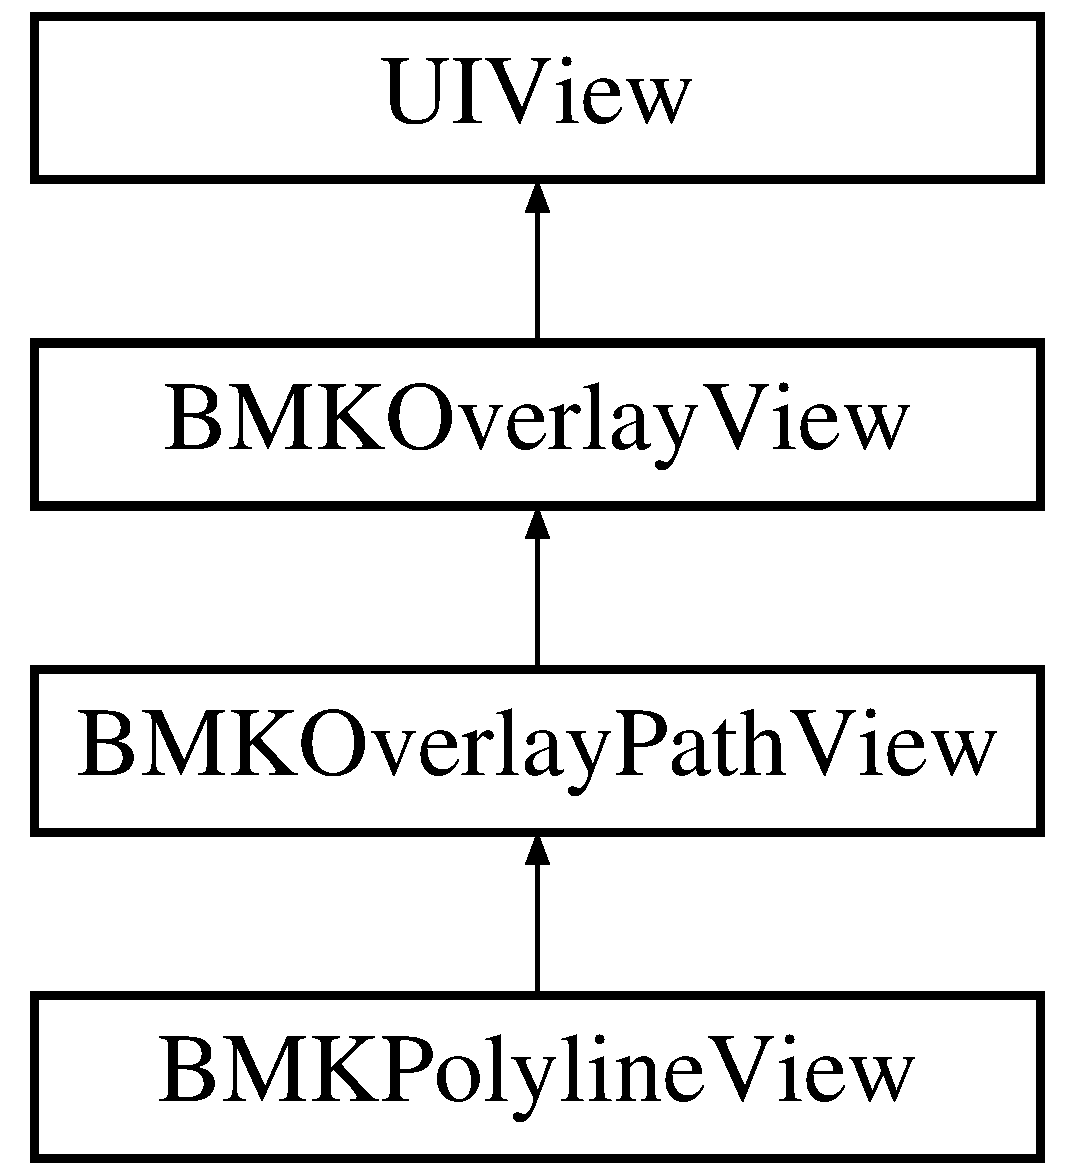
\includegraphics[height=4.000000cm]{interface_b_m_k_polyline_view}
\end{center}
\end{figure}
\subsection*{实例方法}
\begin{DoxyCompactItemize}
\item 
(id) -\/ \hyperlink{interface_b_m_k_polyline_view_a9e771508504ccb0fdf491dcb406e23ed}{init\-With\-Polyline\-:}
\end{DoxyCompactItemize}
\subsection*{Properties}
\begin{DoxyCompactItemize}
\item 
\hypertarget{interface_b_m_k_polyline_view_a780ecfc589530cc4514e790422730e5f}{\hyperlink{interface_b_m_k_polyline}{B\-M\-K\-Polyline} $\ast$ \hyperlink{interface_b_m_k_polyline_view_a780ecfc589530cc4514e790422730e5f}{polyline}}\label{interface_b_m_k_polyline_view_a780ecfc589530cc4514e790422730e5f}

\begin{DoxyCompactList}\small\item\em 该\-View对应的折线数据对象 \end{DoxyCompactList}\end{DoxyCompactItemize}
\subsection*{附加继承成员}


\subsection{详细描述}
此类用于定义一个折线\-View 

\subsection{方法文档}
\hypertarget{interface_b_m_k_polyline_view_a9e771508504ccb0fdf491dcb406e23ed}{\index{B\-M\-K\-Polyline\-View@{B\-M\-K\-Polyline\-View}!init\-With\-Polyline\-:@{init\-With\-Polyline\-:}}
\index{init\-With\-Polyline\-:@{init\-With\-Polyline\-:}!BMKPolylineView@{B\-M\-K\-Polyline\-View}}
\subsubsection[{init\-With\-Polyline\-:}]{\setlength{\rightskip}{0pt plus 5cm}-\/ (id) init\-With\-Polyline\-: 
\begin{DoxyParamCaption}
\item[{({\bf B\-M\-K\-Polyline} $\ast$)}]{polyline}
\end{DoxyParamCaption}
}}\label{interface_b_m_k_polyline_view_a9e771508504ccb0fdf491dcb406e23ed}
根据指定的折线生成一个折线\-View 
\begin{DoxyParams}{参数}
{\em polyline} & 指定的折线数据对象 \\
\hline
\end{DoxyParams}
\begin{DoxyReturn}{返回}
新生成的折线\-View 
\end{DoxyReturn}


The documentation for this class was generated from the following file\-:\begin{DoxyCompactItemize}
\item 
B\-M\-K\-Polyline\-View.\-h\end{DoxyCompactItemize}

\hypertarget{interface_b_m_k_route}{\section{B\-M\-K\-Route 类参考}
\label{interface_b_m_k_route}\index{B\-M\-K\-Route@{B\-M\-K\-Route}}
}


此类表示一条驾驶或步行线路  




{\ttfamily \#import $<$B\-M\-K\-Route\-Search\-Type.\-h$>$}

继承关系图 B\-M\-K\-Route\-:\begin{figure}[H]
\begin{center}
\leavevmode
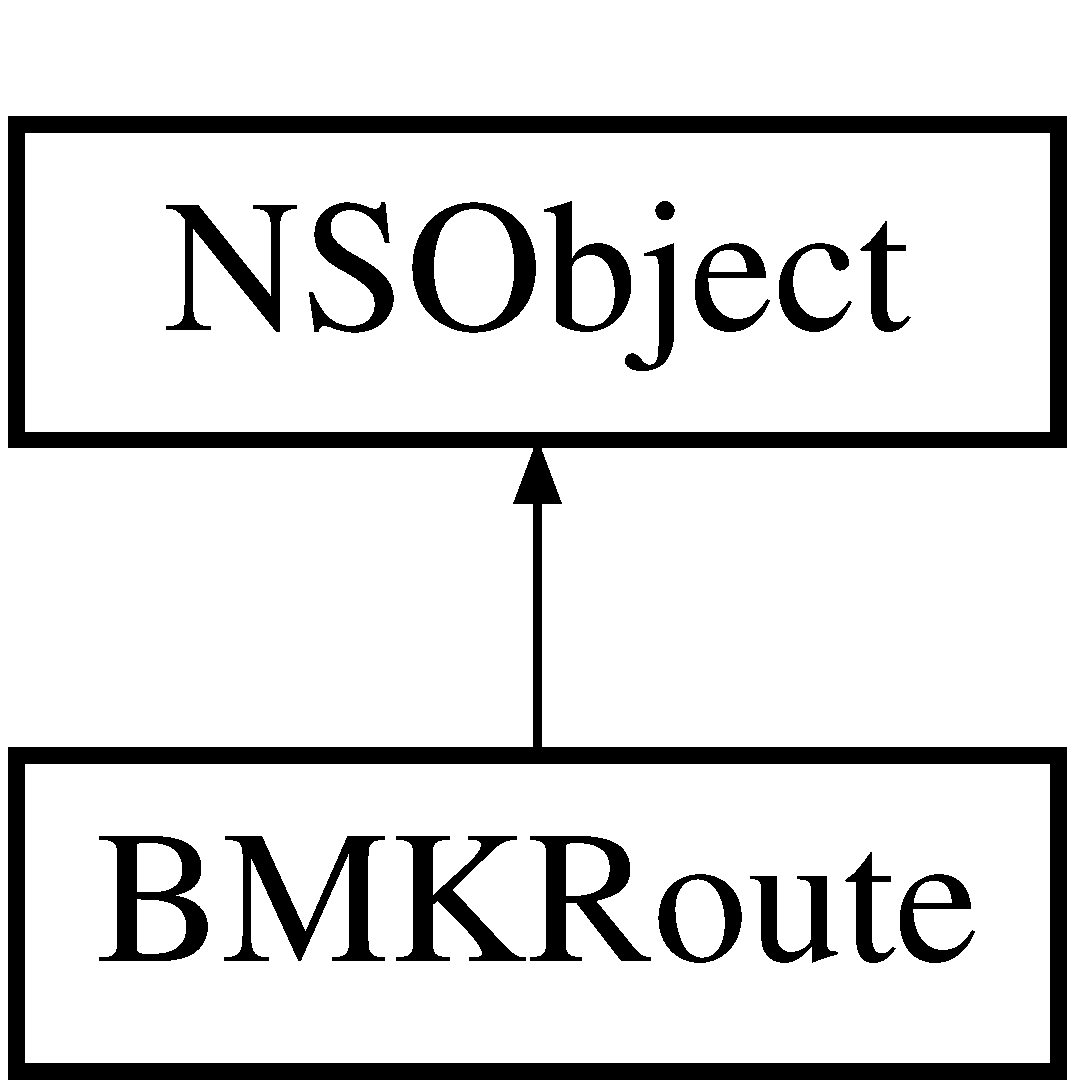
\includegraphics[height=2.000000cm]{interface_b_m_k_route}
\end{center}
\end{figure}
\subsection*{实例方法}
\begin{DoxyCompactItemize}
\item 
\hypertarget{interface_b_m_k_route_a801ea786b1a632afe3ac821ce4d4d4b8}{(int) -\/ \hyperlink{interface_b_m_k_route_a801ea786b1a632afe3ac821ce4d4d4b8}{get\-Points\-Num\-:}}\label{interface_b_m_k_route_a801ea786b1a632afe3ac821ce4d4d4b8}

\begin{DoxyCompactList}\small\item\em 某一段坐标点数目 \end{DoxyCompactList}\item 
\hypertarget{interface_b_m_k_route_ac51eaf7beb1aa2ba6e26a46b953668ee}{(const \hyperlink{struct_b_m_k_map_point}{B\-M\-K\-Map\-Point} $\ast$) -\/ \hyperlink{interface_b_m_k_route_ac51eaf7beb1aa2ba6e26a46b953668ee}{get\-Points\-:}}\label{interface_b_m_k_route_ac51eaf7beb1aa2ba6e26a46b953668ee}

\begin{DoxyCompactList}\small\item\em 某一段坐标点数组 \end{DoxyCompactList}\end{DoxyCompactItemize}
\subsection*{保护成员变量}
\begin{DoxyCompactItemize}
\item 
\hypertarget{interface_b_m_k_route_a76090867eb96a4b86c08ec8c7fc98fce}{int {\bfseries \-\_\-type}}\label{interface_b_m_k_route_a76090867eb96a4b86c08ec8c7fc98fce}

\item 
\hypertarget{interface_b_m_k_route_a8f8c8728df35995a91cd2e43c7ab123e}{C\-L\-Location\-Coordinate2\-D {\bfseries \-\_\-start\-Pt}}\label{interface_b_m_k_route_a8f8c8728df35995a91cd2e43c7ab123e}

\item 
\hypertarget{interface_b_m_k_route_a51b195ee5321cc5d2b7316b8c44ebb83}{C\-L\-Location\-Coordinate2\-D {\bfseries \-\_\-end\-Pt}}\label{interface_b_m_k_route_a51b195ee5321cc5d2b7316b8c44ebb83}

\item 
\hypertarget{interface_b_m_k_route_aa2bf575165b90965d623e3edff14b086}{N\-S\-String $\ast$ {\bfseries \-\_\-tip}}\label{interface_b_m_k_route_aa2bf575165b90965d623e3edff14b086}

\item 
\hypertarget{interface_b_m_k_route_a917e438c9f7b623f47c431842a3cf28b}{int $\ast$ {\bfseries \-\_\-points\-Num}}\label{interface_b_m_k_route_a917e438c9f7b623f47c431842a3cf28b}

\item 
\hypertarget{interface_b_m_k_route_a4d089d8e8dabc41e1d7015ccc53dbaba}{\hyperlink{struct_b_m_k_map_point}{B\-M\-K\-Map\-Point} $\ast$$\ast$ {\bfseries \-\_\-points}}\label{interface_b_m_k_route_a4d089d8e8dabc41e1d7015ccc53dbaba}

\item 
\hypertarget{interface_b_m_k_route_abbea91078abce7b16e66fc37dec39d2d}{int {\bfseries \-\_\-points\-Count}}\label{interface_b_m_k_route_abbea91078abce7b16e66fc37dec39d2d}

\item 
\hypertarget{interface_b_m_k_route_a733a7452324bf21732e119ee70f75e45}{N\-S\-Array $\ast$ {\bfseries \-\_\-steps}}\label{interface_b_m_k_route_a733a7452324bf21732e119ee70f75e45}

\end{DoxyCompactItemize}
\subsection*{Properties}
\begin{DoxyCompactItemize}
\item 
\hypertarget{interface_b_m_k_route_a811a96fafd8ebfde05e6f80ac05c5e76}{int {\bfseries \-\_\-distance}}\label{interface_b_m_k_route_a811a96fafd8ebfde05e6f80ac05c5e76}

\item 
\hypertarget{interface_b_m_k_route_ab8c229e762a5d840a82bf3736c8f571d}{int \hyperlink{interface_b_m_k_route_ab8c229e762a5d840a82bf3736c8f571d}{distance}}\label{interface_b_m_k_route_ab8c229e762a5d840a82bf3736c8f571d}

\begin{DoxyCompactList}\small\item\em 线路距离,单位:米 \end{DoxyCompactList}\item 
\hypertarget{interface_b_m_k_route_a121de8965846b3bf42fd5ea106804c36}{int \hyperlink{interface_b_m_k_route_a121de8965846b3bf42fd5ea106804c36}{type}}\label{interface_b_m_k_route_a121de8965846b3bf42fd5ea106804c36}

\begin{DoxyCompactList}\small\item\em 线路类型,0\-:未知 1\-:驾驶 2\-:步行 \end{DoxyCompactList}\item 
\hypertarget{interface_b_m_k_route_a1598a86af26f5bbc44ae5cb787ed14a6}{int \hyperlink{interface_b_m_k_route_a1598a86af26f5bbc44ae5cb787ed14a6}{points\-Count}}\label{interface_b_m_k_route_a1598a86af26f5bbc44ae5cb787ed14a6}

\begin{DoxyCompactList}\small\item\em 坐标点段数 \end{DoxyCompactList}\item 
\hypertarget{interface_b_m_k_route_a9551046aeaa18a2d2d269186c1417ab5}{C\-L\-Location\-Coordinate2\-D \hyperlink{interface_b_m_k_route_a9551046aeaa18a2d2d269186c1417ab5}{start\-Pt}}\label{interface_b_m_k_route_a9551046aeaa18a2d2d269186c1417ab5}

\begin{DoxyCompactList}\small\item\em 线路起点坐标 \end{DoxyCompactList}\item 
\hypertarget{interface_b_m_k_route_ac101e8dce6365f04d68c3452ea28320a}{C\-L\-Location\-Coordinate2\-D \hyperlink{interface_b_m_k_route_ac101e8dce6365f04d68c3452ea28320a}{end\-Pt}}\label{interface_b_m_k_route_ac101e8dce6365f04d68c3452ea28320a}

\begin{DoxyCompactList}\small\item\em 线路终点坐标 \end{DoxyCompactList}\item 
\hypertarget{interface_b_m_k_route_a3ff9e9bae4c8c883298fe6280c74f109}{N\-S\-String $\ast$ \hyperlink{interface_b_m_k_route_a3ff9e9bae4c8c883298fe6280c74f109}{tip}}\label{interface_b_m_k_route_a3ff9e9bae4c8c883298fe6280c74f109}

\begin{DoxyCompactList}\small\item\em 线路提示 \end{DoxyCompactList}\item 
\hypertarget{interface_b_m_k_route_a2d7c6c1ffbf500845f8f95fc00c1cb4b}{N\-S\-Array $\ast$ \hyperlink{interface_b_m_k_route_a2d7c6c1ffbf500845f8f95fc00c1cb4b}{steps}}\label{interface_b_m_k_route_a2d7c6c1ffbf500845f8f95fc00c1cb4b}

\begin{DoxyCompactList}\small\item\em 线路关键点数组,成员类型为\-B\-M\-K\-Step \end{DoxyCompactList}\item 
\hypertarget{interface_b_m_k_route_a4af51d6046f075f27b3e3402147c785e}{\hyperlink{struct_b_m_k_map_point}{B\-M\-K\-Map\-Point} $\ast$$\ast$ {\bfseries points}}\label{interface_b_m_k_route_a4af51d6046f075f27b3e3402147c785e}

\end{DoxyCompactItemize}


\subsection{详细描述}
此类表示一条驾驶或步行线路 

The documentation for this class was generated from the following file\-:\begin{DoxyCompactItemize}
\item 
B\-M\-K\-Route\-Search\-Type.\-h\end{DoxyCompactItemize}

\hypertarget{interface_b_m_k_route_addr_result}{\section{B\-M\-K\-Route\-Addr\-Result 类参考}
\label{interface_b_m_k_route_addr_result}\index{B\-M\-K\-Route\-Addr\-Result@{B\-M\-K\-Route\-Addr\-Result}}
}


路线搜索地址结果类.\-当输入的起点或终点有多个地点选择时,或者选定的城市没有此地点,但其它城市有(驾乘或步行),返回该类的实例  




{\ttfamily \#import $<$B\-M\-K\-Route\-Search\-Type.\-h$>$}

继承关系图 B\-M\-K\-Route\-Addr\-Result\-:\begin{figure}[H]
\begin{center}
\leavevmode
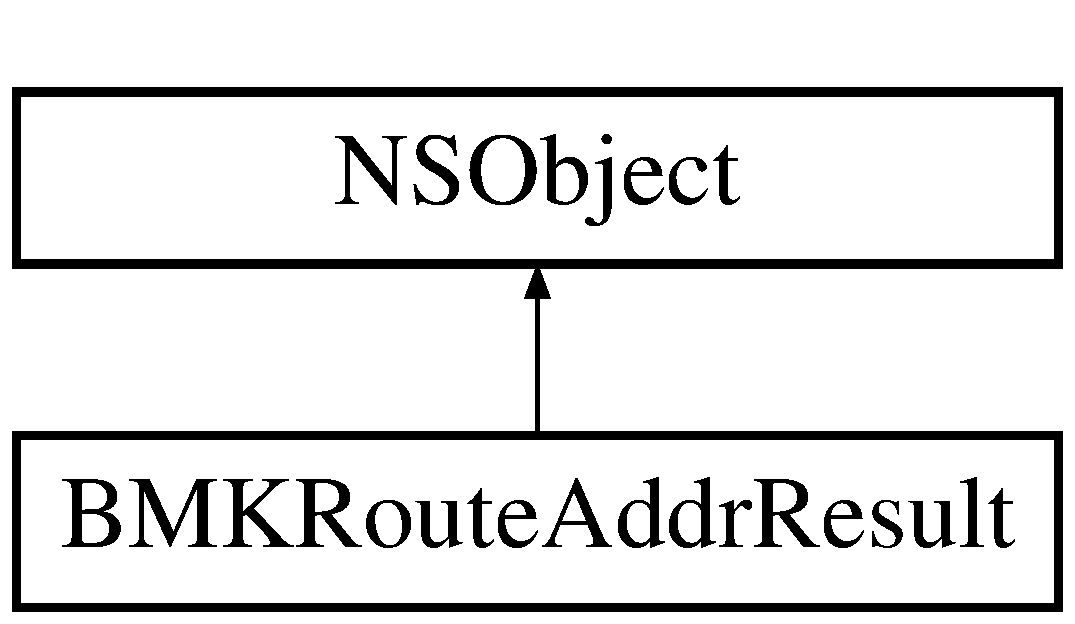
\includegraphics[height=2.000000cm]{interface_b_m_k_route_addr_result}
\end{center}
\end{figure}
\subsection*{保护成员变量}
\begin{DoxyCompactItemize}
\item 
\hypertarget{interface_b_m_k_route_addr_result_a2108d7a47157103e55d409766ab84257}{N\-S\-Array $\ast$ {\bfseries \-\_\-end\-Poi\-List}}\label{interface_b_m_k_route_addr_result_a2108d7a47157103e55d409766ab84257}

\item 
\hypertarget{interface_b_m_k_route_addr_result_ac944121c0903e92a4313a4c0350923cd}{N\-S\-Array $\ast$ {\bfseries \-\_\-start\-City\-List}}\label{interface_b_m_k_route_addr_result_ac944121c0903e92a4313a4c0350923cd}

\item 
\hypertarget{interface_b_m_k_route_addr_result_aed02e5199c20db0c913a1cc6e2d236d9}{N\-S\-Array $\ast$ {\bfseries \-\_\-end\-City\-List}}\label{interface_b_m_k_route_addr_result_aed02e5199c20db0c913a1cc6e2d236d9}

\item 
\hypertarget{interface_b_m_k_route_addr_result_adf21c7d401bfce4af38c94ffc7269d72}{N\-S\-Array $\ast$ {\bfseries \-\_\-way\-Points\-Poi\-List}}\label{interface_b_m_k_route_addr_result_adf21c7d401bfce4af38c94ffc7269d72}

\item 
\hypertarget{interface_b_m_k_route_addr_result_a5799836ee0446e22bac7b39bc5b8945a}{N\-S\-Array $\ast$ {\bfseries \-\_\-way\-Points\-City\-List}}\label{interface_b_m_k_route_addr_result_a5799836ee0446e22bac7b39bc5b8945a}

\end{DoxyCompactItemize}
\subsection*{Properties}
\begin{DoxyCompactItemize}
\item 
\hypertarget{interface_b_m_k_route_addr_result_ad31bb0d912c49be75dad1f61e24a5867}{N\-S\-Array $\ast$ {\bfseries \-\_\-start\-Poi\-List}}\label{interface_b_m_k_route_addr_result_ad31bb0d912c49be75dad1f61e24a5867}

\item 
\hypertarget{interface_b_m_k_route_addr_result_ae29bb91f70c2e6cee75b8a2f918b8fd2}{N\-S\-Array $\ast$ \hyperlink{interface_b_m_k_route_addr_result_ae29bb91f70c2e6cee75b8a2f918b8fd2}{start\-Poi\-List}}\label{interface_b_m_k_route_addr_result_ae29bb91f70c2e6cee75b8a2f918b8fd2}

\begin{DoxyCompactList}\small\item\em 起点\-P\-O\-I列表,成员类型为\-B\-M\-K\-Poi\-Info \end{DoxyCompactList}\item 
\hypertarget{interface_b_m_k_route_addr_result_aac903c422d926b12913133eeb0444e17}{N\-S\-Array $\ast$ \hyperlink{interface_b_m_k_route_addr_result_aac903c422d926b12913133eeb0444e17}{start\-City\-List}}\label{interface_b_m_k_route_addr_result_aac903c422d926b12913133eeb0444e17}

\begin{DoxyCompactList}\small\item\em 起点城市列表,成员类型为\-B\-M\-K\-City\-List\-Info,如果输入的地点在本城市没有而在其它城市有,则返回其它城市的信息 \end{DoxyCompactList}\item 
\hypertarget{interface_b_m_k_route_addr_result_a68f28dd49c16ff67a814d19fe2570e1e}{N\-S\-Array $\ast$ \hyperlink{interface_b_m_k_route_addr_result_a68f28dd49c16ff67a814d19fe2570e1e}{end\-Poi\-List}}\label{interface_b_m_k_route_addr_result_a68f28dd49c16ff67a814d19fe2570e1e}

\begin{DoxyCompactList}\small\item\em 终点\-P\-O\-I列表,成员类型为\-B\-M\-K\-Poi\-Info \end{DoxyCompactList}\item 
\hypertarget{interface_b_m_k_route_addr_result_a29b7a094255410379a8f960c3fc1e3da}{N\-S\-Array $\ast$ \hyperlink{interface_b_m_k_route_addr_result_a29b7a094255410379a8f960c3fc1e3da}{end\-City\-List}}\label{interface_b_m_k_route_addr_result_a29b7a094255410379a8f960c3fc1e3da}

\begin{DoxyCompactList}\small\item\em 终点城市列表,成员类型为\-B\-M\-K\-City\-List\-Info,如果输入的地点在本城市没有而在其它城市有,则返回其它城市的信息 \end{DoxyCompactList}\item 
\hypertarget{interface_b_m_k_route_addr_result_a0724f64a30f591ce225bdf9c9920c70a}{N\-S\-Array $\ast$ \hyperlink{interface_b_m_k_route_addr_result_a0724f64a30f591ce225bdf9c9920c70a}{way\-Point\-Poi\-List}}\label{interface_b_m_k_route_addr_result_a0724f64a30f591ce225bdf9c9920c70a}

\begin{DoxyCompactList}\small\item\em 途经点\-P\-O\-I列表,成员类型为\-N\-S\-Array$<$\-B\-M\-K\-Poi\-Info$\ast$$>$ \end{DoxyCompactList}\item 
\hypertarget{interface_b_m_k_route_addr_result_a11c8c192e86286a080e4df7306800ab8}{N\-S\-Array $\ast$ \hyperlink{interface_b_m_k_route_addr_result_a11c8c192e86286a080e4df7306800ab8}{way\-Point\-City\-List}}\label{interface_b_m_k_route_addr_result_a11c8c192e86286a080e4df7306800ab8}

\begin{DoxyCompactList}\small\item\em 途经点城市列表,成员类型为\-N\-S\-Array$<$\-B\-M\-K\-City\-List\-Info$\ast$$>$,如果输入的地点在本城市没有而在其它城市有,则返回其它城市的信息 \end{DoxyCompactList}\end{DoxyCompactItemize}


\subsection{详细描述}
路线搜索地址结果类.\-当输入的起点或终点有多个地点选择时,或者选定的城市没有此地点,但其它城市有(驾乘或步行),返回该类的实例 

The documentation for this class was generated from the following file\-:\begin{DoxyCompactItemize}
\item 
B\-M\-K\-Route\-Search\-Type.\-h\end{DoxyCompactItemize}

\hypertarget{interface_b_m_k_route_plan}{\section{B\-M\-K\-Route\-Plan 类参考}
\label{interface_b_m_k_route_plan}\index{B\-M\-K\-Route\-Plan@{B\-M\-K\-Route\-Plan}}
}


此类表示一条驾车或步行方案  




{\ttfamily \#import $<$B\-M\-K\-Route\-Search\-Type.\-h$>$}

继承关系图 B\-M\-K\-Route\-Plan\-:\begin{figure}[H]
\begin{center}
\leavevmode
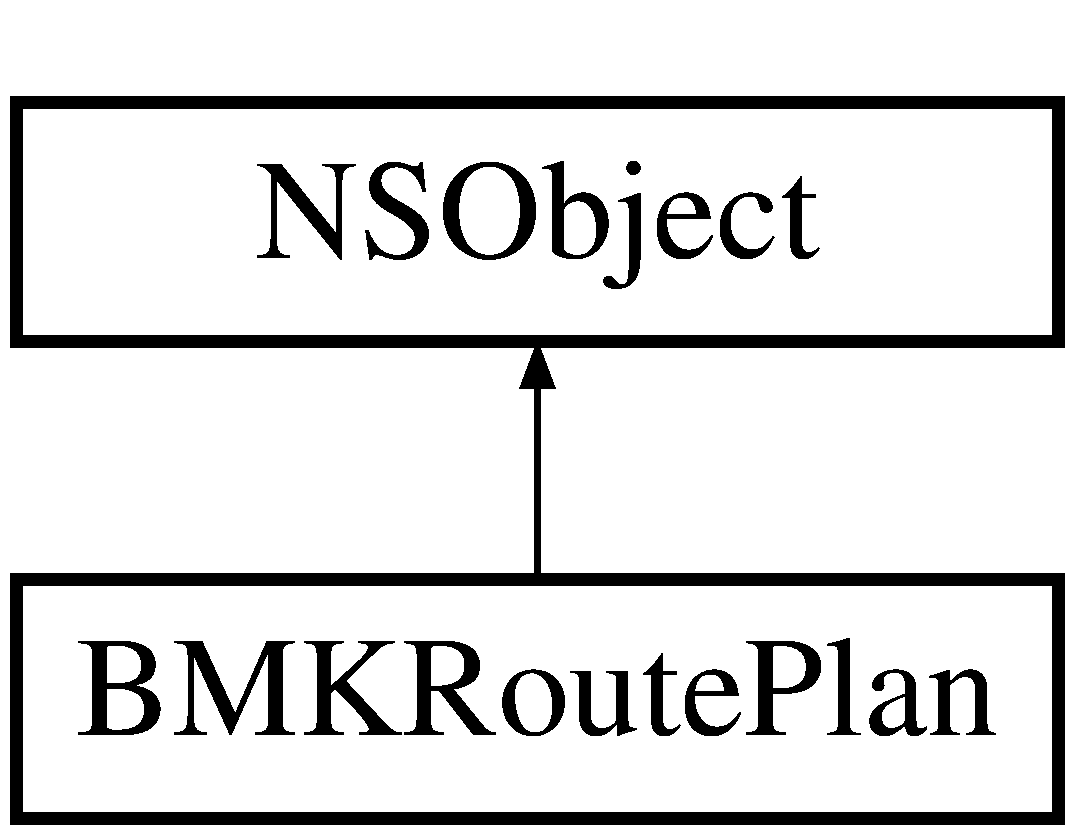
\includegraphics[height=2.000000cm]{interface_b_m_k_route_plan}
\end{center}
\end{figure}
\subsection*{保护成员变量}
\begin{DoxyCompactItemize}
\item 
\hypertarget{interface_b_m_k_route_plan_aa62820a95ab248f113a882b864230135}{N\-S\-Array $\ast$ {\bfseries \-\_\-routes}}\label{interface_b_m_k_route_plan_aa62820a95ab248f113a882b864230135}

\end{DoxyCompactItemize}
\subsection*{Properties}
\begin{DoxyCompactItemize}
\item 
\hypertarget{interface_b_m_k_route_plan_afb7f5f3ff9b33d65172aaf4657d0d0d6}{int {\bfseries \-\_\-distance}}\label{interface_b_m_k_route_plan_afb7f5f3ff9b33d65172aaf4657d0d0d6}

\item 
\hypertarget{interface_b_m_k_route_plan_aa9020d0fe83a58c2192157f47d7930eb}{int \hyperlink{interface_b_m_k_route_plan_aa9020d0fe83a58c2192157f47d7930eb}{distance}}\label{interface_b_m_k_route_plan_aa9020d0fe83a58c2192157f47d7930eb}

\begin{DoxyCompactList}\small\item\em 方案总距离 \end{DoxyCompactList}\item 
\hypertarget{interface_b_m_k_route_plan_a93cd92070e92c4c1a25a8e127bd8b6d5}{N\-S\-Array $\ast$ \hyperlink{interface_b_m_k_route_plan_a93cd92070e92c4c1a25a8e127bd8b6d5}{routes}}\label{interface_b_m_k_route_plan_a93cd92070e92c4c1a25a8e127bd8b6d5}

\begin{DoxyCompactList}\small\item\em B\-M\-K\-Route数组 \end{DoxyCompactList}\end{DoxyCompactItemize}


\subsection{详细描述}
此类表示一条驾车或步行方案 

The documentation for this class was generated from the following file\-:\begin{DoxyCompactItemize}
\item 
B\-M\-K\-Route\-Search\-Type.\-h\end{DoxyCompactItemize}

\hypertarget{interface_b_m_k_search}{\section{B\-M\-K\-Search 类参考}
\label{interface_b_m_k_search}\index{B\-M\-K\-Search@{B\-M\-K\-Search}}
}


搜索服务  




{\ttfamily \#import $<$B\-M\-K\-Search.\-h$>$}

继承关系图 B\-M\-K\-Search\-:\begin{figure}[H]
\begin{center}
\leavevmode
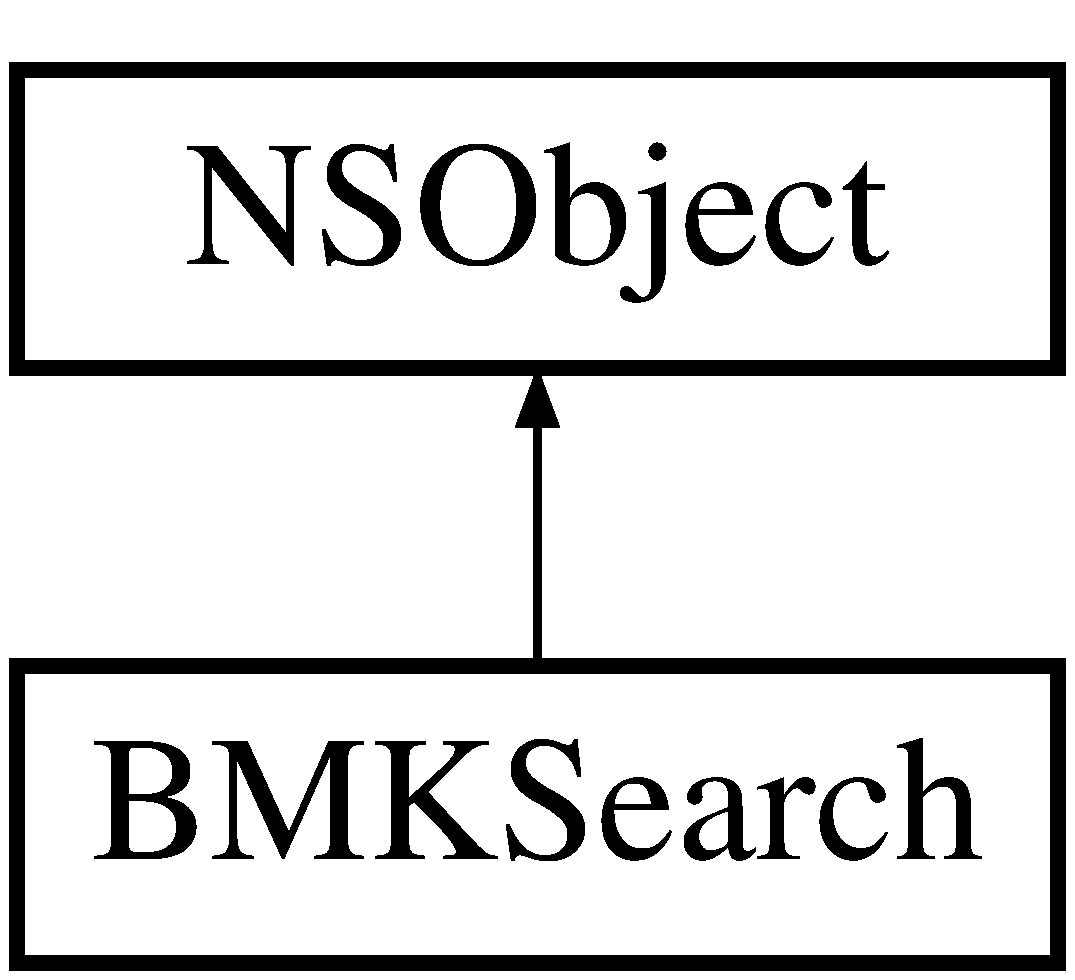
\includegraphics[height=2.000000cm]{interface_b_m_k_search}
\end{center}
\end{figure}
\subsection*{实例方法}
\begin{DoxyCompactItemize}
\item 
(B\-O\-O\-L) -\/ \hyperlink{interface_b_m_k_search_a3d4be019a638b79bff6c95081e624b24}{poi\-Search\-In\-City\-:with\-Key\-:page\-Index\-:}
\item 
(B\-O\-O\-L) -\/ \hyperlink{interface_b_m_k_search_a905ca1d5f5b829d9759903234b359657}{poi\-Search\-Inbounds\-:left\-Bottom\-:right\-Top\-:page\-Index\-:}
\item 
(B\-O\-O\-L) -\/ \hyperlink{interface_b_m_k_search_ad57823f0c67cfa45180b69299b546351}{poi\-Search\-Near\-By\-:center\-:radius\-:page\-Index\-:}
\item 
(B\-O\-O\-L) -\/ \hyperlink{interface_b_m_k_search_a2c2eacd43a31175dfcc1d4c6d89e0498}{transit\-Search\-:start\-Node\-:end\-Node\-:}
\item 
(B\-O\-O\-L) -\/ \hyperlink{interface_b_m_k_search_a20e8105eea18c931b4f7d5f75cefbf09}{driving\-Search\-:start\-Node\-:end\-City\-:end\-Node\-:}
\item 
(B\-O\-O\-L) -\/ \hyperlink{interface_b_m_k_search_acc6e736e62cdafd5a1daa94d75071642}{driving\-Search\-:start\-Node\-:end\-City\-:end\-Node\-:through\-Way\-Points\-:}
\item 
(B\-O\-O\-L) -\/ \hyperlink{interface_b_m_k_search_aa2a9b0f69520e4e17ff9504d10e77f57}{walking\-Search\-:start\-Node\-:end\-City\-:end\-Node\-:}
\item 
(B\-O\-O\-L) -\/ \hyperlink{interface_b_m_k_search_ae5169b6362dda612ffd1f1b5f9df6137}{reverse\-Geocode\-:}
\item 
(B\-O\-O\-L) -\/ \hyperlink{interface_b_m_k_search_a5bd9e45d6d8042585428d5bdde0b584b}{geocode\-:with\-City\-:}
\item 
(B\-O\-O\-L) -\/ \hyperlink{interface_b_m_k_search_a8d4b04f2d17b67229b59bf6224bdee7a}{suggestion\-Search\-:}
\item 
(B\-O\-O\-L) -\/ \hyperlink{interface_b_m_k_search_a4d0b7ec9e07dd5493e14de39edf852d0}{suggestion\-Search\-:in\-City\-:}
\item 
(B\-O\-O\-L) -\/ \hyperlink{interface_b_m_k_search_ac6256527dd532f554d02410cef13caf8}{bus\-Line\-Search\-:with\-Key\-:}
\end{DoxyCompactItemize}
\subsection*{类方法}
\begin{DoxyCompactItemize}
\item 
(void) + \hyperlink{interface_b_m_k_search_a18442a7afac76b21535d175189b7d2ec}{set\-Page\-Capacity\-:}
\item 
(int) + \hyperlink{interface_b_m_k_search_a21e67fb54e22bfdca495490f3bfa731d}{get\-Page\-Capacity}
\end{DoxyCompactItemize}
\subsection*{Properties}
\begin{DoxyCompactItemize}
\item 
\hypertarget{interface_b_m_k_search_ad3b8fc2fe55c02166fb2a7953cdbc8d7}{id$<$ \hyperlink{protocol_b_m_k_search_delegate-p}{B\-M\-K\-Search\-Delegate} $>$ \hyperlink{interface_b_m_k_search_ad3b8fc2fe55c02166fb2a7953cdbc8d7}{delegate}}\label{interface_b_m_k_search_ad3b8fc2fe55c02166fb2a7953cdbc8d7}

\begin{DoxyCompactList}\small\item\em 检索模块的\-Delegate,此处记得不用的时候需要置nil,否则影响内存的释放 \end{DoxyCompactList}\item 
\hypertarget{interface_b_m_k_search_a070e0b90d93a92c1642e9390af7164ed}{int \hyperlink{interface_b_m_k_search_a070e0b90d93a92c1642e9390af7164ed}{transit\-Policy}}\label{interface_b_m_k_search_a070e0b90d93a92c1642e9390af7164ed}

\begin{DoxyCompactList}\small\item\em 公交检索策略 \end{DoxyCompactList}\item 
\hypertarget{interface_b_m_k_search_a7bbc7acb0020ab8d5d600ce423805606}{int \hyperlink{interface_b_m_k_search_a7bbc7acb0020ab8d5d600ce423805606}{driving\-Policy}}\label{interface_b_m_k_search_a7bbc7acb0020ab8d5d600ce423805606}

\begin{DoxyCompactList}\small\item\em 驾乘检索策略 \end{DoxyCompactList}\end{DoxyCompactItemize}


\subsection{详细描述}
搜索服务 

\subsection{方法文档}
\hypertarget{interface_b_m_k_search_ac6256527dd532f554d02410cef13caf8}{\index{B\-M\-K\-Search@{B\-M\-K\-Search}!bus\-Line\-Search\-:with\-Key\-:@{bus\-Line\-Search\-:with\-Key\-:}}
\index{bus\-Line\-Search\-:with\-Key\-:@{bus\-Line\-Search\-:with\-Key\-:}!BMKSearch@{B\-M\-K\-Search}}
\subsubsection[{bus\-Line\-Search\-:with\-Key\-:}]{\setlength{\rightskip}{0pt plus 5cm}-\/ (B\-O\-O\-L) bus\-Line\-Search\-: 
\begin{DoxyParamCaption}
\item[{(N\-S\-String $\ast$)}]{city}
\item[{withKey:(N\-S\-String $\ast$)}]{bus\-Line\-Uid}
\end{DoxyParamCaption}
}}\label{interface_b_m_k_search_ac6256527dd532f554d02410cef13caf8}
公交详情检索 异步函数,返回结果在\-B\-M\-K\-Search\-Delegate的on\-Get\-Bus\-Detail\-Result通知 
\begin{DoxyParams}{参数}
{\em city} & 城市名,用于在哪个城市内进行检索 \\
\hline
{\em bus\-Line\-Uid} & 公交线路的uid \\
\hline
\end{DoxyParams}
\begin{DoxyReturn}{返回}
成功返回\-Y\-E\-S,否则返回\-N\-O 
\end{DoxyReturn}
\hypertarget{interface_b_m_k_search_a20e8105eea18c931b4f7d5f75cefbf09}{\index{B\-M\-K\-Search@{B\-M\-K\-Search}!driving\-Search\-:start\-Node\-:end\-City\-:end\-Node\-:@{driving\-Search\-:start\-Node\-:end\-City\-:end\-Node\-:}}
\index{driving\-Search\-:start\-Node\-:end\-City\-:end\-Node\-:@{driving\-Search\-:start\-Node\-:end\-City\-:end\-Node\-:}!BMKSearch@{B\-M\-K\-Search}}
\subsubsection[{driving\-Search\-:start\-Node\-:end\-City\-:end\-Node\-:}]{\setlength{\rightskip}{0pt plus 5cm}-\/ (B\-O\-O\-L) driving\-Search\-: 
\begin{DoxyParamCaption}
\item[{(N\-S\-String $\ast$)}]{start\-City}
\item[{startNode:({\bf B\-M\-K\-Plan\-Node} $\ast$)}]{start}
\item[{endCity:(N\-S\-String $\ast$)}]{end\-City}
\item[{endNode:({\bf B\-M\-K\-Plan\-Node} $\ast$)}]{end}
\end{DoxyParamCaption}
}}\label{interface_b_m_k_search_a20e8105eea18c931b4f7d5f75cefbf09}
驾乘路线检索 异步函数,返回结果在\-B\-M\-K\-Search\-Delegate的on\-Get\-Driving\-Route\-Result通知 
\begin{DoxyParams}{参数}
{\em start\-City} & 起点所在城市,起点为坐标时可不填 \\
\hline
{\em start} & 检索的起点,可通过关键字、坐标两种方式指定 \\
\hline
{\em end\-City} & 终点所在城市,终点为坐标时可不填 \\
\hline
{\em end} & 检索的终点,可通过关键字、坐标两种方式指定 \\
\hline
\end{DoxyParams}
\begin{DoxyReturn}{返回}
成功返回\-Y\-E\-S,否则返回\-N\-O 
\end{DoxyReturn}
\hypertarget{interface_b_m_k_search_acc6e736e62cdafd5a1daa94d75071642}{\index{B\-M\-K\-Search@{B\-M\-K\-Search}!driving\-Search\-:start\-Node\-:end\-City\-:end\-Node\-:through\-Way\-Points\-:@{driving\-Search\-:start\-Node\-:end\-City\-:end\-Node\-:through\-Way\-Points\-:}}
\index{driving\-Search\-:start\-Node\-:end\-City\-:end\-Node\-:through\-Way\-Points\-:@{driving\-Search\-:start\-Node\-:end\-City\-:end\-Node\-:through\-Way\-Points\-:}!BMKSearch@{B\-M\-K\-Search}}
\subsubsection[{driving\-Search\-:start\-Node\-:end\-City\-:end\-Node\-:through\-Way\-Points\-:}]{\setlength{\rightskip}{0pt plus 5cm}-\/ (B\-O\-O\-L) driving\-Search\-: 
\begin{DoxyParamCaption}
\item[{(N\-S\-String $\ast$)}]{start\-City}
\item[{startNode:({\bf B\-M\-K\-Plan\-Node} $\ast$)}]{start}
\item[{endCity:(N\-S\-String $\ast$)}]{end\-City}
\item[{endNode:({\bf B\-M\-K\-Plan\-Node} $\ast$)}]{end}
\item[{throughWayPoints:(N\-S\-Array $\ast$)}]{way\-Points\-Array}
\end{DoxyParamCaption}
}}\label{interface_b_m_k_search_acc6e736e62cdafd5a1daa94d75071642}
驾乘路线检索 异步函数,返回结果在\-B\-M\-K\-Search\-Delegate的on\-Get\-Driving\-Route\-Result通知 
\begin{DoxyParams}{参数}
{\em start\-City} & 起点所在城市,起点为坐标时可不填 \\
\hline
{\em start} & 检索的起点,可通过关键字、坐标两种方式指定 \\
\hline
{\em end\-City} & 终点所在城市,终点为坐标时可不填 \\
\hline
{\em end} & 检索的终点,可通过关键字、坐标两种方式指定 \\
\hline
{\em way\-Points\-Array} & 途经点数组,存储\-B\-M\-K\-Plan\-Node信息的节点。way\-Points\-Array为nil或空时,表示没有途经点。最多支持10个途经点,超过10个请求发送不成功。 \\
\hline
\end{DoxyParams}
\begin{DoxyReturn}{返回}
成功返回\-Y\-E\-S,否则返回\-N\-O 
\end{DoxyReturn}
\hypertarget{interface_b_m_k_search_a5bd9e45d6d8042585428d5bdde0b584b}{\index{B\-M\-K\-Search@{B\-M\-K\-Search}!geocode\-:with\-City\-:@{geocode\-:with\-City\-:}}
\index{geocode\-:with\-City\-:@{geocode\-:with\-City\-:}!BMKSearch@{B\-M\-K\-Search}}
\subsubsection[{geocode\-:with\-City\-:}]{\setlength{\rightskip}{0pt plus 5cm}-\/ (B\-O\-O\-L) geocode\-: 
\begin{DoxyParamCaption}
\item[{(N\-S\-String $\ast$)}]{addr}
\item[{withCity:(N\-S\-String $\ast$)}]{city}
\end{DoxyParamCaption}
}}\label{interface_b_m_k_search_a5bd9e45d6d8042585428d5bdde0b584b}
根据地址名称获取地理信息 异步函数,返回结果在\-B\-M\-K\-Search\-Delegate的on\-Get\-Geocode\-Result通知 \begin{DoxyReturn}{返回}
成功返回\-Y\-E\-S,否则返回\-N\-O 
\end{DoxyReturn}
\hypertarget{interface_b_m_k_search_a21e67fb54e22bfdca495490f3bfa731d}{\index{B\-M\-K\-Search@{B\-M\-K\-Search}!get\-Page\-Capacity@{get\-Page\-Capacity}}
\index{get\-Page\-Capacity@{get\-Page\-Capacity}!BMKSearch@{B\-M\-K\-Search}}
\subsubsection[{get\-Page\-Capacity}]{\setlength{\rightskip}{0pt plus 5cm}+ (int) get\-Page\-Capacity 
\begin{DoxyParamCaption}
{}
\end{DoxyParamCaption}
}}\label{interface_b_m_k_search_a21e67fb54e22bfdca495490f3bfa731d}
返回每页容量 \begin{DoxyReturn}{返回}
每页容量 
\end{DoxyReturn}
\hypertarget{interface_b_m_k_search_a905ca1d5f5b829d9759903234b359657}{\index{B\-M\-K\-Search@{B\-M\-K\-Search}!poi\-Search\-Inbounds\-:left\-Bottom\-:right\-Top\-:page\-Index\-:@{poi\-Search\-Inbounds\-:left\-Bottom\-:right\-Top\-:page\-Index\-:}}
\index{poi\-Search\-Inbounds\-:left\-Bottom\-:right\-Top\-:page\-Index\-:@{poi\-Search\-Inbounds\-:left\-Bottom\-:right\-Top\-:page\-Index\-:}!BMKSearch@{B\-M\-K\-Search}}
\subsubsection[{poi\-Search\-Inbounds\-:left\-Bottom\-:right\-Top\-:page\-Index\-:}]{\setlength{\rightskip}{0pt plus 5cm}-\/ (B\-O\-O\-L) poi\-Search\-Inbounds\-: 
\begin{DoxyParamCaption}
\item[{(N\-S\-String $\ast$)}]{key}
\item[{leftBottom:(C\-L\-Location\-Coordinate2\-D)}]{pt\-L\-B}
\item[{rightTop:(C\-L\-Location\-Coordinate2\-D)}]{pt\-R\-T}
\item[{pageIndex:(int)}]{index}
\end{DoxyParamCaption}
}}\label{interface_b_m_k_search_a905ca1d5f5b829d9759903234b359657}
根据范围和检索词发起范围检索 异步函数,返回结果在\-B\-M\-K\-Search\-Delegate的on\-Get\-Poi\-Result通知 
\begin{DoxyParams}{参数}
{\em key} & 关键词 \\
\hline
{\em pt\-L\-B} & 地理坐标,范围的左下角 \\
\hline
{\em pt\-R\-B} & 地理坐标,范围的右下角 \\
\hline
{\em index} & 页码,如果是第一次发起搜索,填0,根据返回的结果可以去获取第n页的结果,页码从0开始 \\
\hline
\end{DoxyParams}
\begin{DoxyReturn}{返回}
成功返回\-Y\-E\-S,否则返回\-N\-O 
\end{DoxyReturn}
\hypertarget{interface_b_m_k_search_a3d4be019a638b79bff6c95081e624b24}{\index{B\-M\-K\-Search@{B\-M\-K\-Search}!poi\-Search\-In\-City\-:with\-Key\-:page\-Index\-:@{poi\-Search\-In\-City\-:with\-Key\-:page\-Index\-:}}
\index{poi\-Search\-In\-City\-:with\-Key\-:page\-Index\-:@{poi\-Search\-In\-City\-:with\-Key\-:page\-Index\-:}!BMKSearch@{B\-M\-K\-Search}}
\subsubsection[{poi\-Search\-In\-City\-:with\-Key\-:page\-Index\-:}]{\setlength{\rightskip}{0pt plus 5cm}-\/ (B\-O\-O\-L) poi\-Search\-In\-City\-: 
\begin{DoxyParamCaption}
\item[{(N\-S\-String $\ast$)}]{city}
\item[{withKey:(N\-S\-String $\ast$)}]{key}
\item[{pageIndex:(int)}]{index}
\end{DoxyParamCaption}
}}\label{interface_b_m_k_search_a3d4be019a638b79bff6c95081e624b24}
城市\-P\-O\-I检索 异步函数,返回结果在\-B\-M\-K\-Search\-Delegate的on\-Get\-Poi\-Result通知 
\begin{DoxyParams}{参数}
{\em city} & 城市名,如果为nil则在当前底图范围搜索 \\
\hline
{\em key} & 关键词 \\
\hline
{\em index} & 页码,如果是第一次发起搜索,填0,根据返回的结果可以去获取第n页的结果,页码从0开始 \\
\hline
\end{DoxyParams}
\begin{DoxyReturn}{返回}
成功返回\-Y\-E\-S,否则返回\-N\-O 
\end{DoxyReturn}
\hypertarget{interface_b_m_k_search_ad57823f0c67cfa45180b69299b546351}{\index{B\-M\-K\-Search@{B\-M\-K\-Search}!poi\-Search\-Near\-By\-:center\-:radius\-:page\-Index\-:@{poi\-Search\-Near\-By\-:center\-:radius\-:page\-Index\-:}}
\index{poi\-Search\-Near\-By\-:center\-:radius\-:page\-Index\-:@{poi\-Search\-Near\-By\-:center\-:radius\-:page\-Index\-:}!BMKSearch@{B\-M\-K\-Search}}
\subsubsection[{poi\-Search\-Near\-By\-:center\-:radius\-:page\-Index\-:}]{\setlength{\rightskip}{0pt plus 5cm}-\/ (B\-O\-O\-L) poi\-Search\-Near\-By\-: 
\begin{DoxyParamCaption}
\item[{(N\-S\-String $\ast$)}]{key}
\item[{center:(C\-L\-Location\-Coordinate2\-D)}]{pt\-Center}
\item[{radius:(int)}]{radius}
\item[{pageIndex:(int)}]{index}
\end{DoxyParamCaption}
}}\label{interface_b_m_k_search_ad57823f0c67cfa45180b69299b546351}
根据范围和检索词发起范围检索 异步函数,返回结果在\-B\-M\-K\-Search\-Delegate的on\-Get\-Poi\-Result通知 
\begin{DoxyParams}{参数}
{\em keys} & 关键词列表,必须大于1个,小于等于10个 \\
\hline
{\em pt\-L\-B} & 地理坐标,范围的左下角 \\
\hline
{\em pt\-R\-B} & 地理坐标,范围的右下角 \\
\hline
{\em index} & 页码,如果是第一次发起搜索,填0,根据返回的结果可以去获取第n页的结果,页码从0开始 \\
\hline
\end{DoxyParams}
\begin{DoxyReturn}{返回}
成功返回\-Y\-E\-S,否则返回\-N\-O 根据中心点、半径和检索词发起周边检索 异步函数,返回结果在\-B\-M\-K\-Search\-Delegate的on\-Get\-Poi\-Result通知 
\end{DoxyReturn}

\begin{DoxyParams}{参数}
{\em key} & 关键词 \\
\hline
{\em pt\-Center} & 中心点地理坐标 \\
\hline
{\em radius} & 半径,单位:米 必须大于0 \\
\hline
{\em index} & 页码,如果是第一次发起搜索,填0,根据返回的结果可以去获取第n页的结果,页码从0开始 \\
\hline
\end{DoxyParams}
\begin{DoxyReturn}{返回}
成功返回\-Y\-E\-S,否则返回\-N\-O 
\end{DoxyReturn}
\hypertarget{interface_b_m_k_search_ae5169b6362dda612ffd1f1b5f9df6137}{\index{B\-M\-K\-Search@{B\-M\-K\-Search}!reverse\-Geocode\-:@{reverse\-Geocode\-:}}
\index{reverse\-Geocode\-:@{reverse\-Geocode\-:}!BMKSearch@{B\-M\-K\-Search}}
\subsubsection[{reverse\-Geocode\-:}]{\setlength{\rightskip}{0pt plus 5cm}-\/ (B\-O\-O\-L) reverse\-Geocode\-: 
\begin{DoxyParamCaption}
\item[{(C\-L\-Location\-Coordinate2\-D)}]{center}
\end{DoxyParamCaption}
}}\label{interface_b_m_k_search_ae5169b6362dda612ffd1f1b5f9df6137}
根据地理坐标获取地址信息 异步函数,返回结果在\-B\-M\-K\-Search\-Delegate的on\-Get\-Addr\-Result通知 \begin{DoxyReturn}{返回}
成功返回\-Y\-E\-S,否则返回\-N\-O 
\end{DoxyReturn}
\hypertarget{interface_b_m_k_search_a18442a7afac76b21535d175189b7d2ec}{\index{B\-M\-K\-Search@{B\-M\-K\-Search}!set\-Page\-Capacity\-:@{set\-Page\-Capacity\-:}}
\index{set\-Page\-Capacity\-:@{set\-Page\-Capacity\-:}!BMKSearch@{B\-M\-K\-Search}}
\subsubsection[{set\-Page\-Capacity\-:}]{\setlength{\rightskip}{0pt plus 5cm}+ (void) set\-Page\-Capacity\-: 
\begin{DoxyParamCaption}
\item[{(int)}]{capacity}
\end{DoxyParamCaption}
}}\label{interface_b_m_k_search_a18442a7afac76b21535d175189b7d2ec}
设置每页容量 支持1-\/50.对下一次检索有效 
\begin{DoxyParams}{参数}
{\em capacity} & 指定的每页\-P\-O\-I最大数目 \\
\hline
\end{DoxyParams}
\hypertarget{interface_b_m_k_search_a8d4b04f2d17b67229b59bf6224bdee7a}{\index{B\-M\-K\-Search@{B\-M\-K\-Search}!suggestion\-Search\-:@{suggestion\-Search\-:}}
\index{suggestion\-Search\-:@{suggestion\-Search\-:}!BMKSearch@{B\-M\-K\-Search}}
\subsubsection[{suggestion\-Search\-:}]{\setlength{\rightskip}{0pt plus 5cm}-\/ (B\-O\-O\-L) suggestion\-Search\-: 
\begin{DoxyParamCaption}
\item[{(N\-S\-String $\ast$)}]{key}
\end{DoxyParamCaption}
}}\label{interface_b_m_k_search_a8d4b04f2d17b67229b59bf6224bdee7a}
异步函数,返回结果在\-B\-M\-K\-Search\-Delegate的on\-Get\-Suggestion\-Result通知 \begin{DoxyReturn}{返回}
成功返回\-Y\-E\-S,否则返回\-N\-O 
\end{DoxyReturn}
\hypertarget{interface_b_m_k_search_a4d0b7ec9e07dd5493e14de39edf852d0}{\index{B\-M\-K\-Search@{B\-M\-K\-Search}!suggestion\-Search\-:in\-City\-:@{suggestion\-Search\-:in\-City\-:}}
\index{suggestion\-Search\-:in\-City\-:@{suggestion\-Search\-:in\-City\-:}!BMKSearch@{B\-M\-K\-Search}}
\subsubsection[{suggestion\-Search\-:in\-City\-:}]{\setlength{\rightskip}{0pt plus 5cm}-\/ (B\-O\-O\-L) {\bf suggestion\-Search\-:} 
\begin{DoxyParamCaption}
\item[{(N\-S\-String $\ast$)}]{key}
\item[{inCity:(N\-S\-String $\ast$)}]{cityname}
\end{DoxyParamCaption}
}}\label{interface_b_m_k_search_a4d0b7ec9e07dd5493e14de39edf852d0}
异步函数,返回结果在\-B\-M\-K\-Search\-Delegate的on\-Get\-Suggestion\-Result通知 
\begin{DoxyParams}{参数}
{\em cityname} & 城市名,用于指定在特定城市内检索 \\
\hline
\end{DoxyParams}
\begin{DoxyReturn}{返回}
成功返回\-Y\-E\-S,否则返回\-N\-O 
\end{DoxyReturn}
\hypertarget{interface_b_m_k_search_a2c2eacd43a31175dfcc1d4c6d89e0498}{\index{B\-M\-K\-Search@{B\-M\-K\-Search}!transit\-Search\-:start\-Node\-:end\-Node\-:@{transit\-Search\-:start\-Node\-:end\-Node\-:}}
\index{transit\-Search\-:start\-Node\-:end\-Node\-:@{transit\-Search\-:start\-Node\-:end\-Node\-:}!BMKSearch@{B\-M\-K\-Search}}
\subsubsection[{transit\-Search\-:start\-Node\-:end\-Node\-:}]{\setlength{\rightskip}{0pt plus 5cm}-\/ (B\-O\-O\-L) transit\-Search\-: 
\begin{DoxyParamCaption}
\item[{(N\-S\-String $\ast$)}]{city}
\item[{startNode:({\bf B\-M\-K\-Plan\-Node} $\ast$)}]{start}
\item[{endNode:({\bf B\-M\-K\-Plan\-Node} $\ast$)}]{end}
\end{DoxyParamCaption}
}}\label{interface_b_m_k_search_a2c2eacd43a31175dfcc1d4c6d89e0498}
根据中心点、半径和检索词发起周边检索 异步函数,返回结果在\-B\-M\-K\-Search\-Delegate的on\-Get\-Poi\-Result通知 
\begin{DoxyParams}{参数}
{\em keys} & 关键词列表,必须大于1个,小于等于10个 \\
\hline
{\em pt\-Center} & 中心点地理坐标 \\
\hline
{\em radius} & 半径,单位:米 必须大于0 \\
\hline
{\em index} & 页码,如果是第一次发起搜索,填0,根据返回的结果可以去获取第n页的结果,页码从0开始 \\
\hline
\end{DoxyParams}
\begin{DoxyReturn}{返回}
成功返回\-Y\-E\-S,否则返回\-N\-O 公交路线检索 异步函数,返回结果在\-B\-M\-K\-Search\-Delegate的on\-Get\-Transit\-Route\-Result通知 
\end{DoxyReturn}

\begin{DoxyParams}{参数}
{\em city} & 城市名,用于在哪个城市内进行检索 \\
\hline
{\em start} & 检索的起点,可通过关键字、坐标两种方式指定 \\
\hline
{\em end} & 检索的终点,可通过关键字、坐标两种方式指定 \\
\hline
\end{DoxyParams}
\begin{DoxyReturn}{返回}
成功返回\-Y\-E\-S,否则返回\-N\-O 
\end{DoxyReturn}
\hypertarget{interface_b_m_k_search_aa2a9b0f69520e4e17ff9504d10e77f57}{\index{B\-M\-K\-Search@{B\-M\-K\-Search}!walking\-Search\-:start\-Node\-:end\-City\-:end\-Node\-:@{walking\-Search\-:start\-Node\-:end\-City\-:end\-Node\-:}}
\index{walking\-Search\-:start\-Node\-:end\-City\-:end\-Node\-:@{walking\-Search\-:start\-Node\-:end\-City\-:end\-Node\-:}!BMKSearch@{B\-M\-K\-Search}}
\subsubsection[{walking\-Search\-:start\-Node\-:end\-City\-:end\-Node\-:}]{\setlength{\rightskip}{0pt plus 5cm}-\/ (B\-O\-O\-L) walking\-Search\-: 
\begin{DoxyParamCaption}
\item[{(N\-S\-String $\ast$)}]{start\-City}
\item[{startNode:({\bf B\-M\-K\-Plan\-Node} $\ast$)}]{start}
\item[{endCity:(N\-S\-String $\ast$)}]{end\-City}
\item[{endNode:({\bf B\-M\-K\-Plan\-Node} $\ast$)}]{end}
\end{DoxyParamCaption}
}}\label{interface_b_m_k_search_aa2a9b0f69520e4e17ff9504d10e77f57}
步行路线检索 异步函数,返回结果在\-B\-M\-K\-Search\-Delegate的on\-Get\-Walking\-Route\-Result通知 
\begin{DoxyParams}{参数}
{\em start\-City} & 起点所在城市,起点为坐标时可不填 \\
\hline
{\em start} & 检索的起点,可通过关键字、坐标两种方式指定 \\
\hline
{\em end\-City} & 终点所在城市,终点为坐标时可不填 \\
\hline
{\em end} & 检索的终点,可通过关键字、坐标两种方式指定 \\
\hline
\end{DoxyParams}
\begin{DoxyReturn}{返回}
成功返回\-Y\-E\-S,否则返回\-N\-O 
\end{DoxyReturn}


The documentation for this class was generated from the following file\-:\begin{DoxyCompactItemize}
\item 
B\-M\-K\-Search.\-h\end{DoxyCompactItemize}

\hypertarget{protocol_b_m_k_search_delegate-p}{\section{$<$B\-M\-K\-Search\-Delegate$>$ 协议参考}
\label{protocol_b_m_k_search_delegate-p}\index{$<$\-B\-M\-K\-Search\-Delegate$>$@{$<$\-B\-M\-K\-Search\-Delegate$>$}}
}


搜索delegate,用于获取搜索结果  




{\ttfamily \#import $<$B\-M\-K\-Search.\-h$>$}

继承关系图 $<$B\-M\-K\-Search\-Delegate$>$\-:\begin{figure}[H]
\begin{center}
\leavevmode
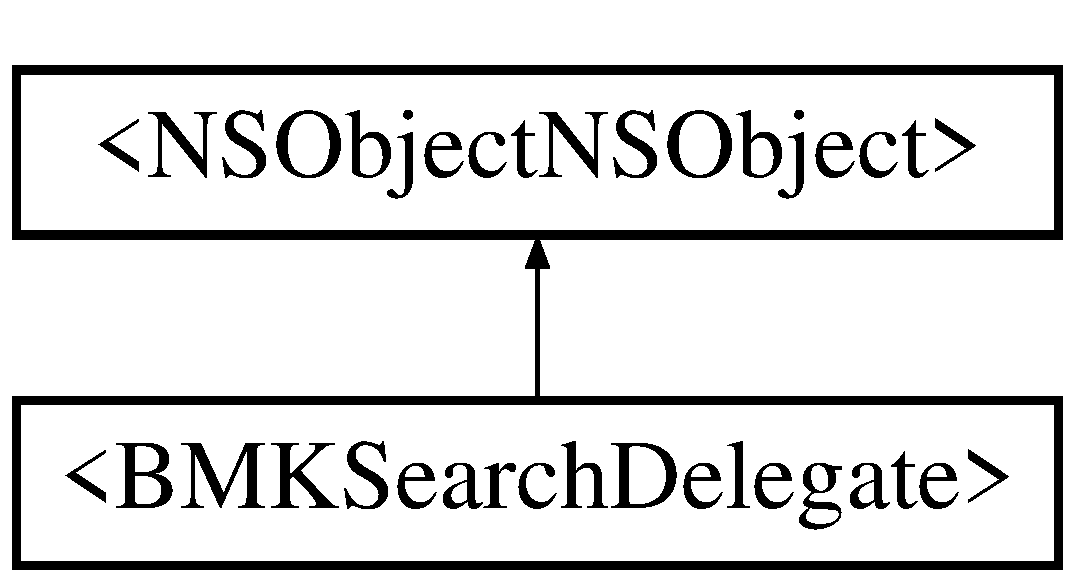
\includegraphics[height=2.000000cm]{protocol_b_m_k_search_delegate-p}
\end{center}
\end{figure}
\subsection*{实例方法}
\begin{DoxyCompactItemize}
\item 
(void) -\/ \hyperlink{protocol_b_m_k_search_delegate-p_aaebc1737d2df985b3d7878fd9ea53122}{on\-Get\-Poi\-Result\-:search\-Type\-:error\-Code\-:}
\item 
(void) -\/ \hyperlink{protocol_b_m_k_search_delegate-p_a300f82b22ee2295fb1eda590ce468f6e}{on\-Get\-Transit\-Route\-Result\-:error\-Code\-:}
\item 
(void) -\/ \hyperlink{protocol_b_m_k_search_delegate-p_ae37ff980770f8d8b1129e41cc05c76ae}{on\-Get\-Driving\-Route\-Result\-:error\-Code\-:}
\item 
(void) -\/ \hyperlink{protocol_b_m_k_search_delegate-p_a4fcbf962b5af9d50c194a69da26261c1}{on\-Get\-Walking\-Route\-Result\-:error\-Code\-:}
\item 
(void) -\/ \hyperlink{protocol_b_m_k_search_delegate-p_a7eebe5b2da7524f72e9f56413647d2fc}{on\-Get\-Addr\-Result\-:error\-Code\-:}
\item 
(void) -\/ \hyperlink{protocol_b_m_k_search_delegate-p_a029cc846020073395c4c437798ccfa05}{on\-Get\-Suggestion\-Result\-:error\-Code\-:}
\item 
(void) -\/ \hyperlink{protocol_b_m_k_search_delegate-p_aa43e8862315533032603901acaaf8dca}{on\-Get\-Bus\-Detail\-Result\-:error\-Code\-:}
\end{DoxyCompactItemize}


\subsection{详细描述}
搜索delegate,用于获取搜索结果 

\subsection{方法文档}
\hypertarget{protocol_b_m_k_search_delegate-p_a7eebe5b2da7524f72e9f56413647d2fc}{\index{B\-M\-K\-Search\-Delegate-\/p@{B\-M\-K\-Search\-Delegate-\/p}!on\-Get\-Addr\-Result\-:error\-Code\-:@{on\-Get\-Addr\-Result\-:error\-Code\-:}}
\index{on\-Get\-Addr\-Result\-:error\-Code\-:@{on\-Get\-Addr\-Result\-:error\-Code\-:}!BMKSearchDelegate-p@{B\-M\-K\-Search\-Delegate-\/p}}
\subsubsection[{on\-Get\-Addr\-Result\-:error\-Code\-:}]{\setlength{\rightskip}{0pt plus 5cm}-\/ (void) on\-Get\-Addr\-Result\-: 
\begin{DoxyParamCaption}
\item[{({\bf B\-M\-K\-Addr\-Info} $\ast$)}]{result}
\item[{errorCode:(int)}]{error}
\end{DoxyParamCaption}
\hspace{0.3cm}{\ttfamily [optional]}}}\label{protocol_b_m_k_search_delegate-p_a7eebe5b2da7524f72e9f56413647d2fc}
返回地址信息搜索结果 
\begin{DoxyParams}{参数}
{\em result} & 搜索结果 \\
\hline
{\em error} & 错误号,\\
\hline
\end{DoxyParams}
\begin{DoxySeeAlso}{See Also}
B\-M\-K\-Error\-Code 
\end{DoxySeeAlso}
\hypertarget{protocol_b_m_k_search_delegate-p_aa43e8862315533032603901acaaf8dca}{\index{B\-M\-K\-Search\-Delegate-\/p@{B\-M\-K\-Search\-Delegate-\/p}!on\-Get\-Bus\-Detail\-Result\-:error\-Code\-:@{on\-Get\-Bus\-Detail\-Result\-:error\-Code\-:}}
\index{on\-Get\-Bus\-Detail\-Result\-:error\-Code\-:@{on\-Get\-Bus\-Detail\-Result\-:error\-Code\-:}!BMKSearchDelegate-p@{B\-M\-K\-Search\-Delegate-\/p}}
\subsubsection[{on\-Get\-Bus\-Detail\-Result\-:error\-Code\-:}]{\setlength{\rightskip}{0pt plus 5cm}-\/ (void) on\-Get\-Bus\-Detail\-Result\-: 
\begin{DoxyParamCaption}
\item[{({\bf B\-M\-K\-Bus\-Line\-Result} $\ast$)}]{bus\-Line\-Result}
\item[{errorCode:(int)}]{error}
\end{DoxyParamCaption}
\hspace{0.3cm}{\ttfamily [optional]}}}\label{protocol_b_m_k_search_delegate-p_aa43e8862315533032603901acaaf8dca}
返回busdetail搜索结果 
\begin{DoxyParams}{参数}
{\em bus\-Line\-Result} & 搜索结果 \\
\hline
{\em error} & 错误号,\\
\hline
\end{DoxyParams}
\begin{DoxySeeAlso}{See Also}
B\-M\-K\-Error\-Code 
\end{DoxySeeAlso}
\hypertarget{protocol_b_m_k_search_delegate-p_ae37ff980770f8d8b1129e41cc05c76ae}{\index{B\-M\-K\-Search\-Delegate-\/p@{B\-M\-K\-Search\-Delegate-\/p}!on\-Get\-Driving\-Route\-Result\-:error\-Code\-:@{on\-Get\-Driving\-Route\-Result\-:error\-Code\-:}}
\index{on\-Get\-Driving\-Route\-Result\-:error\-Code\-:@{on\-Get\-Driving\-Route\-Result\-:error\-Code\-:}!BMKSearchDelegate-p@{B\-M\-K\-Search\-Delegate-\/p}}
\subsubsection[{on\-Get\-Driving\-Route\-Result\-:error\-Code\-:}]{\setlength{\rightskip}{0pt plus 5cm}-\/ (void) on\-Get\-Driving\-Route\-Result\-: 
\begin{DoxyParamCaption}
\item[{({\bf B\-M\-K\-Plan\-Result} $\ast$)}]{result}
\item[{errorCode:(int)}]{error}
\end{DoxyParamCaption}
\hspace{0.3cm}{\ttfamily [optional]}}}\label{protocol_b_m_k_search_delegate-p_ae37ff980770f8d8b1129e41cc05c76ae}
返回驾乘搜索结果 
\begin{DoxyParams}{参数}
{\em result} & 搜索结果 \\
\hline
{\em error} & 错误号,\\
\hline
\end{DoxyParams}
\begin{DoxySeeAlso}{See Also}
B\-M\-K\-Error\-Code 
\end{DoxySeeAlso}
\hypertarget{protocol_b_m_k_search_delegate-p_aaebc1737d2df985b3d7878fd9ea53122}{\index{B\-M\-K\-Search\-Delegate-\/p@{B\-M\-K\-Search\-Delegate-\/p}!on\-Get\-Poi\-Result\-:search\-Type\-:error\-Code\-:@{on\-Get\-Poi\-Result\-:search\-Type\-:error\-Code\-:}}
\index{on\-Get\-Poi\-Result\-:search\-Type\-:error\-Code\-:@{on\-Get\-Poi\-Result\-:search\-Type\-:error\-Code\-:}!BMKSearchDelegate-p@{B\-M\-K\-Search\-Delegate-\/p}}
\subsubsection[{on\-Get\-Poi\-Result\-:search\-Type\-:error\-Code\-:}]{\setlength{\rightskip}{0pt plus 5cm}-\/ (void) on\-Get\-Poi\-Result\-: 
\begin{DoxyParamCaption}
\item[{(N\-S\-Array $\ast$)}]{poi\-Result\-List}
\item[{searchType:(int)}]{type}
\item[{errorCode:(int)}]{error}
\end{DoxyParamCaption}
\hspace{0.3cm}{\ttfamily [optional]}}}\label{protocol_b_m_k_search_delegate-p_aaebc1737d2df985b3d7878fd9ea53122}
返回\-P\-O\-I搜索结果 
\begin{DoxyParams}{参数}
{\em poi\-Result\-List} & 搜索结果列表,成员类型为\-B\-M\-K\-Poi\-Result \\
\hline
{\em type} & 返回结果类型: B\-M\-K\-Type\-Poi\-List,B\-M\-K\-Type\-Area\-Poi\-List,B\-M\-K\-Area\-Multi\-Poi\-List \\
\hline
{\em error} & 错误号,\\
\hline
\end{DoxyParams}
\begin{DoxySeeAlso}{See Also}
B\-M\-K\-Error\-Code 
\end{DoxySeeAlso}
\hypertarget{protocol_b_m_k_search_delegate-p_a029cc846020073395c4c437798ccfa05}{\index{B\-M\-K\-Search\-Delegate-\/p@{B\-M\-K\-Search\-Delegate-\/p}!on\-Get\-Suggestion\-Result\-:error\-Code\-:@{on\-Get\-Suggestion\-Result\-:error\-Code\-:}}
\index{on\-Get\-Suggestion\-Result\-:error\-Code\-:@{on\-Get\-Suggestion\-Result\-:error\-Code\-:}!BMKSearchDelegate-p@{B\-M\-K\-Search\-Delegate-\/p}}
\subsubsection[{on\-Get\-Suggestion\-Result\-:error\-Code\-:}]{\setlength{\rightskip}{0pt plus 5cm}-\/ (void) on\-Get\-Suggestion\-Result\-: 
\begin{DoxyParamCaption}
\item[{({\bf B\-M\-K\-Suggestion\-Result} $\ast$)}]{result}
\item[{errorCode:(int)}]{error}
\end{DoxyParamCaption}
\hspace{0.3cm}{\ttfamily [optional]}}}\label{protocol_b_m_k_search_delegate-p_a029cc846020073395c4c437798ccfa05}
返回suggestion搜索结果 
\begin{DoxyParams}{参数}
{\em result} & 搜索结果 \\
\hline
{\em error} & 错误号,\\
\hline
\end{DoxyParams}
\begin{DoxySeeAlso}{See Also}
B\-M\-K\-Error\-Code 
\end{DoxySeeAlso}
\hypertarget{protocol_b_m_k_search_delegate-p_a300f82b22ee2295fb1eda590ce468f6e}{\index{B\-M\-K\-Search\-Delegate-\/p@{B\-M\-K\-Search\-Delegate-\/p}!on\-Get\-Transit\-Route\-Result\-:error\-Code\-:@{on\-Get\-Transit\-Route\-Result\-:error\-Code\-:}}
\index{on\-Get\-Transit\-Route\-Result\-:error\-Code\-:@{on\-Get\-Transit\-Route\-Result\-:error\-Code\-:}!BMKSearchDelegate-p@{B\-M\-K\-Search\-Delegate-\/p}}
\subsubsection[{on\-Get\-Transit\-Route\-Result\-:error\-Code\-:}]{\setlength{\rightskip}{0pt plus 5cm}-\/ (void) on\-Get\-Transit\-Route\-Result\-: 
\begin{DoxyParamCaption}
\item[{({\bf B\-M\-K\-Plan\-Result} $\ast$)}]{result}
\item[{errorCode:(int)}]{error}
\end{DoxyParamCaption}
\hspace{0.3cm}{\ttfamily [optional]}}}\label{protocol_b_m_k_search_delegate-p_a300f82b22ee2295fb1eda590ce468f6e}
返回公交搜索结果 
\begin{DoxyParams}{参数}
{\em result} & 搜索结果 \\
\hline
{\em error} & 错误号,\\
\hline
\end{DoxyParams}
\begin{DoxySeeAlso}{See Also}
B\-M\-K\-Error\-Code 
\end{DoxySeeAlso}
\hypertarget{protocol_b_m_k_search_delegate-p_a4fcbf962b5af9d50c194a69da26261c1}{\index{B\-M\-K\-Search\-Delegate-\/p@{B\-M\-K\-Search\-Delegate-\/p}!on\-Get\-Walking\-Route\-Result\-:error\-Code\-:@{on\-Get\-Walking\-Route\-Result\-:error\-Code\-:}}
\index{on\-Get\-Walking\-Route\-Result\-:error\-Code\-:@{on\-Get\-Walking\-Route\-Result\-:error\-Code\-:}!BMKSearchDelegate-p@{B\-M\-K\-Search\-Delegate-\/p}}
\subsubsection[{on\-Get\-Walking\-Route\-Result\-:error\-Code\-:}]{\setlength{\rightskip}{0pt plus 5cm}-\/ (void) on\-Get\-Walking\-Route\-Result\-: 
\begin{DoxyParamCaption}
\item[{({\bf B\-M\-K\-Plan\-Result} $\ast$)}]{result}
\item[{errorCode:(int)}]{error}
\end{DoxyParamCaption}
\hspace{0.3cm}{\ttfamily [optional]}}}\label{protocol_b_m_k_search_delegate-p_a4fcbf962b5af9d50c194a69da26261c1}
返回步行搜索结果 
\begin{DoxyParams}{参数}
{\em result} & 搜索结果 \\
\hline
{\em error} & 错误号,\\
\hline
\end{DoxyParams}
\begin{DoxySeeAlso}{See Also}
B\-M\-K\-Error\-Code 
\end{DoxySeeAlso}


The documentation for this protocol was generated from the following file\-:\begin{DoxyCompactItemize}
\item 
B\-M\-K\-Search.\-h\end{DoxyCompactItemize}

\hypertarget{interface_b_m_k_shape}{\section{B\-M\-K\-Shape 类参考}
\label{interface_b_m_k_shape}\index{B\-M\-K\-Shape@{B\-M\-K\-Shape}}
}


该类为一个抽象类,定义了基于\-B\-M\-K\-Annotation的\-B\-M\-K\-Shape类的基本属性和行为,不能直接使用,必须子类化之后才能使用  




{\ttfamily \#import $<$B\-M\-K\-Shape.\-h$>$}

继承关系图 B\-M\-K\-Shape\-:\begin{figure}[H]
\begin{center}
\leavevmode
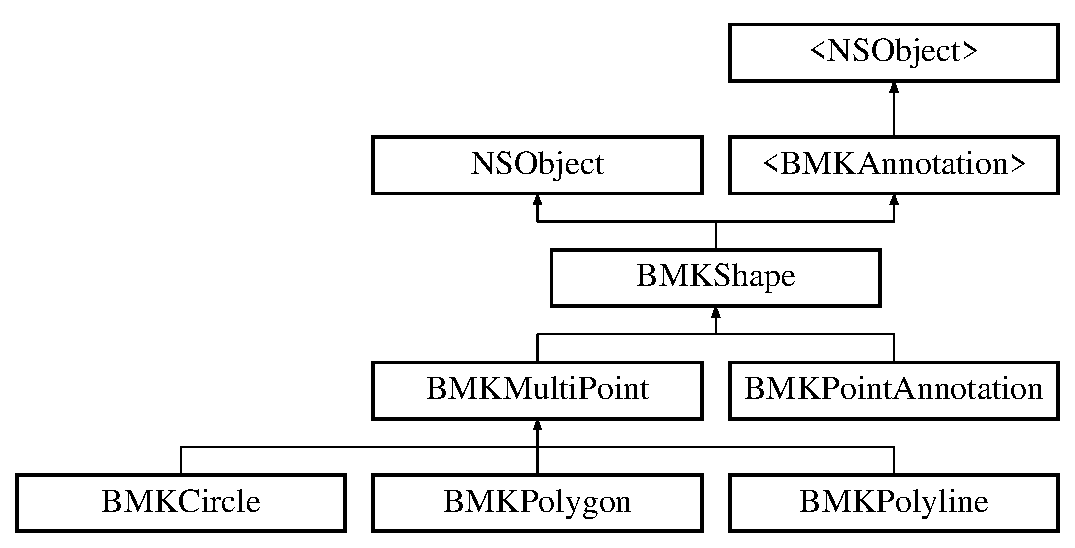
\includegraphics[height=5.000000cm]{interface_b_m_k_shape}
\end{center}
\end{figure}
\subsection*{保护成员变量}
\begin{DoxyCompactItemize}
\item 
\hypertarget{interface_b_m_k_shape_ac6113f6e339e61ca616a82b28876a6db}{package N\-S\-String $\ast$ {\bfseries \-\_\-title}}\label{interface_b_m_k_shape_ac6113f6e339e61ca616a82b28876a6db}

\item 
\hypertarget{interface_b_m_k_shape_a0fe1968032511a58adec771ae3ab143d}{N\-S\-String $\ast$ {\bfseries \-\_\-subtitle}}\label{interface_b_m_k_shape_a0fe1968032511a58adec771ae3ab143d}

\end{DoxyCompactItemize}
\subsection*{Properties}
\begin{DoxyCompactItemize}
\item 
\hypertarget{interface_b_m_k_shape_a64da6d2885114c0c2da35aa1ffec925d}{N\-S\-String $\ast$ \hyperlink{interface_b_m_k_shape_a64da6d2885114c0c2da35aa1ffec925d}{title}}\label{interface_b_m_k_shape_a64da6d2885114c0c2da35aa1ffec925d}

\begin{DoxyCompactList}\small\item\em 要显示的标题 \end{DoxyCompactList}\item 
\hypertarget{interface_b_m_k_shape_ae588ba39a27b52bcaed14d40e6494398}{N\-S\-String $\ast$ \hyperlink{interface_b_m_k_shape_ae588ba39a27b52bcaed14d40e6494398}{subtitle}}\label{interface_b_m_k_shape_ae588ba39a27b52bcaed14d40e6494398}

\begin{DoxyCompactList}\small\item\em 要显示的副标题 \end{DoxyCompactList}\end{DoxyCompactItemize}
\subsection*{附加继承成员}


\subsection{详细描述}
该类为一个抽象类,定义了基于\-B\-M\-K\-Annotation的\-B\-M\-K\-Shape类的基本属性和行为,不能直接使用,必须子类化之后才能使用 

The documentation for this class was generated from the following file\-:\begin{DoxyCompactItemize}
\item 
B\-M\-K\-Shape.\-h\end{DoxyCompactItemize}

\hypertarget{interface_b_m_k_step}{\section{B\-M\-K\-Step 类参考}
\label{interface_b_m_k_step}\index{B\-M\-K\-Step@{B\-M\-K\-Step}}
}


此类表示驾车或步行路线中的一个关键点  




{\ttfamily \#import $<$B\-M\-K\-Route\-Search\-Type.\-h$>$}

继承关系图 B\-M\-K\-Step\-:\begin{figure}[H]
\begin{center}
\leavevmode
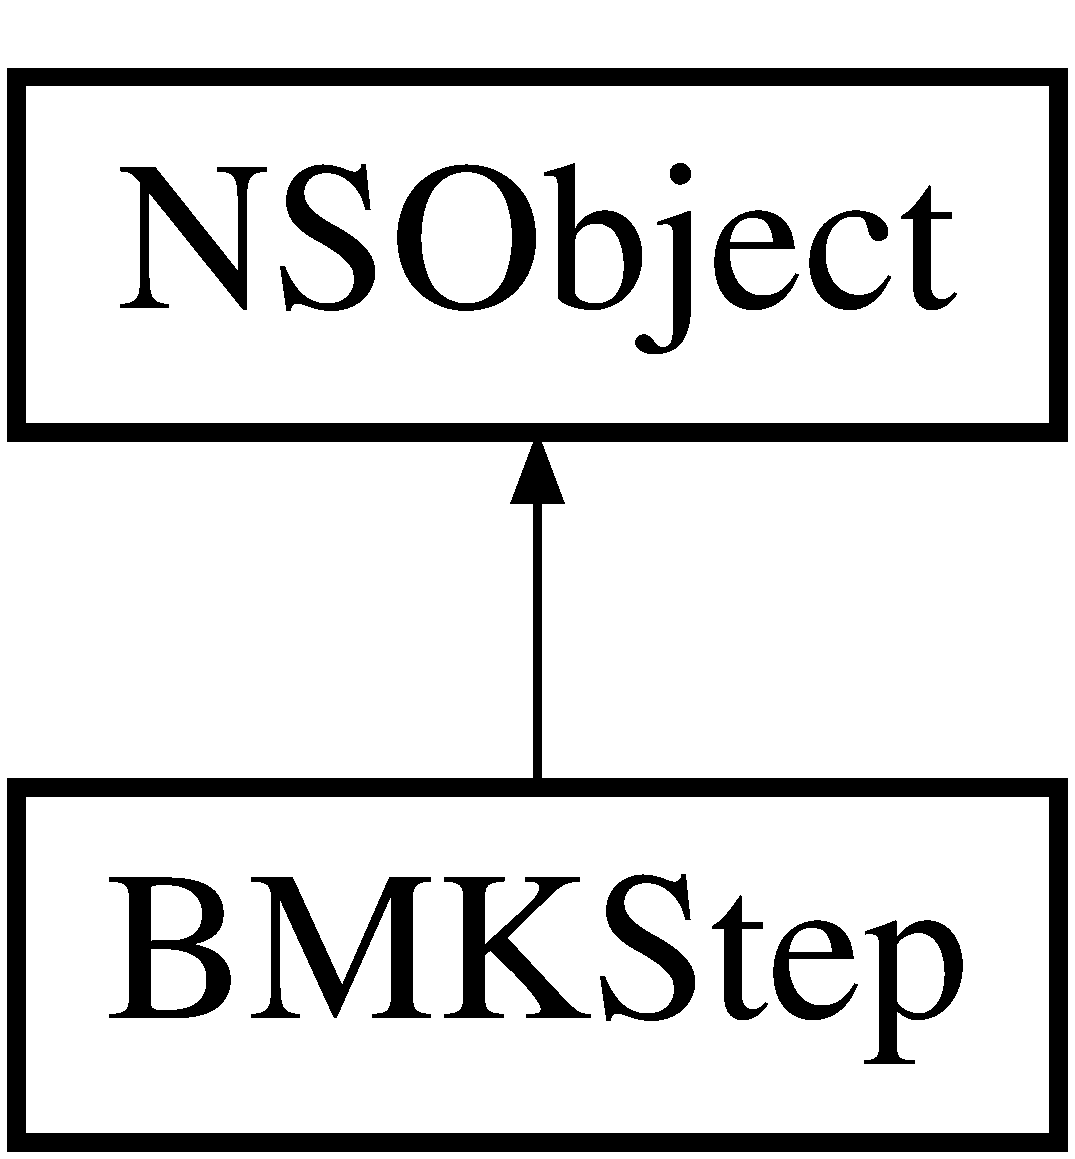
\includegraphics[height=2.000000cm]{interface_b_m_k_step}
\end{center}
\end{figure}
\subsection*{保护成员变量}
\begin{DoxyCompactItemize}
\item 
\hypertarget{interface_b_m_k_step_a230932a6c5fc5fe1f58720c7ecc1db5f}{C\-L\-Location\-Coordinate2\-D {\bfseries \-\_\-pt}}\label{interface_b_m_k_step_a230932a6c5fc5fe1f58720c7ecc1db5f}

\item 
\hypertarget{interface_b_m_k_step_aaec82a08f562e79fd6e71a5c4c8564f4}{N\-S\-String $\ast$ {\bfseries \-\_\-content}}\label{interface_b_m_k_step_aaec82a08f562e79fd6e71a5c4c8564f4}

\item 
\hypertarget{interface_b_m_k_step_ab33cdca63bee56baaf844b19274d80fb}{int {\bfseries \-\_\-degree}}\label{interface_b_m_k_step_ab33cdca63bee56baaf844b19274d80fb}

\end{DoxyCompactItemize}
\subsection*{Properties}
\begin{DoxyCompactItemize}
\item 
\hypertarget{interface_b_m_k_step_ad517bf5db8d177cb33cd94489dbaac51}{C\-L\-Location\-Coordinate2\-D \hyperlink{interface_b_m_k_step_ad517bf5db8d177cb33cd94489dbaac51}{pt}}\label{interface_b_m_k_step_ad517bf5db8d177cb33cd94489dbaac51}

\begin{DoxyCompactList}\small\item\em 关键点坐标 \end{DoxyCompactList}\item 
\hypertarget{interface_b_m_k_step_a647dc013ca983bb77a6d0f4407ee1d63}{N\-S\-String $\ast$ \hyperlink{interface_b_m_k_step_a647dc013ca983bb77a6d0f4407ee1d63}{content}}\label{interface_b_m_k_step_a647dc013ca983bb77a6d0f4407ee1d63}

\begin{DoxyCompactList}\small\item\em 关键点提示信息 \end{DoxyCompactList}\item 
\hypertarget{interface_b_m_k_step_a072bddb98bea4d5da2d6a5f54df46599}{int \hyperlink{interface_b_m_k_step_a072bddb98bea4d5da2d6a5f54df46599}{degree}}\label{interface_b_m_k_step_a072bddb98bea4d5da2d6a5f54df46599}

\begin{DoxyCompactList}\small\item\em 路线相对正北的角度 \end{DoxyCompactList}\end{DoxyCompactItemize}


\subsection{详细描述}
此类表示驾车或步行路线中的一个关键点 

The documentation for this class was generated from the following file\-:\begin{DoxyCompactItemize}
\item 
B\-M\-K\-Route\-Search\-Type.\-h\end{DoxyCompactItemize}

\hypertarget{interface_b_m_k_suggestion_result}{\section{B\-M\-K\-Suggestion\-Result 类参考}
\label{interface_b_m_k_suggestion_result}\index{B\-M\-K\-Suggestion\-Result@{B\-M\-K\-Suggestion\-Result}}
}


Suggestion结果类  




{\ttfamily \#import $<$B\-M\-K\-Poi\-Search\-Type.\-h$>$}

继承关系图 B\-M\-K\-Suggestion\-Result\-:\begin{figure}[H]
\begin{center}
\leavevmode
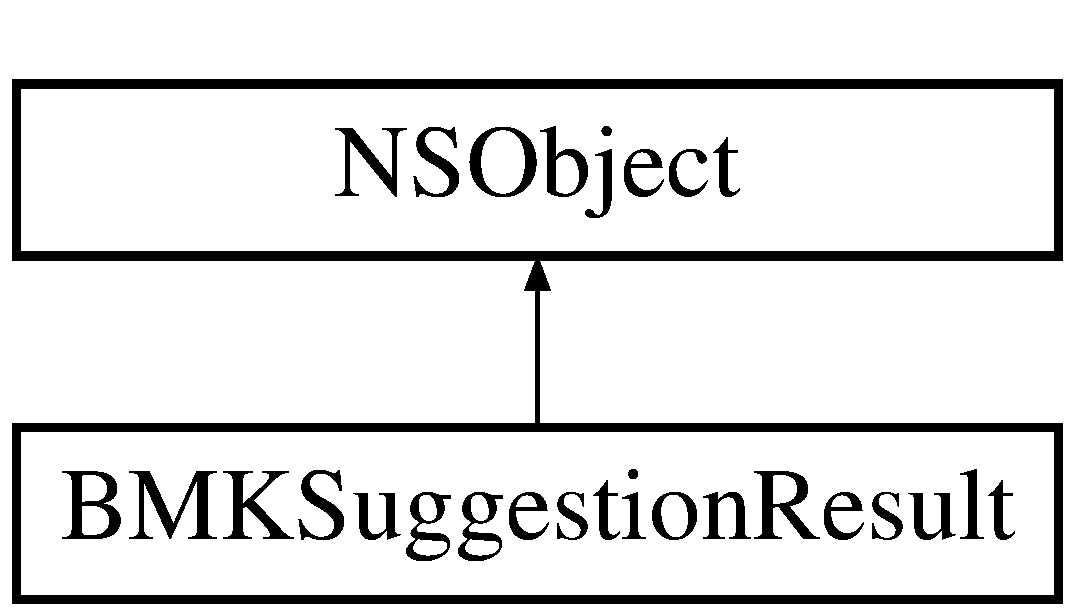
\includegraphics[height=2.000000cm]{interface_b_m_k_suggestion_result}
\end{center}
\end{figure}
\subsection*{保护成员变量}
\begin{DoxyCompactItemize}
\item 
\hypertarget{interface_b_m_k_suggestion_result_a6b3b6f1702dbb6acbe1d77e71d5b07b5}{N\-S\-Array $\ast$ {\bfseries \-\_\-city\-List}}\label{interface_b_m_k_suggestion_result_a6b3b6f1702dbb6acbe1d77e71d5b07b5}

\item 
\hypertarget{interface_b_m_k_suggestion_result_a0d6c54df02825f8166ff6c55c95b8770}{N\-S\-Array $\ast$ {\bfseries \-\_\-district\-List}}\label{interface_b_m_k_suggestion_result_a0d6c54df02825f8166ff6c55c95b8770}

\end{DoxyCompactItemize}
\subsection*{Properties}
\begin{DoxyCompactItemize}
\item 
\hypertarget{interface_b_m_k_suggestion_result_af33171b4e254408d71e6e6904ff361a1}{N\-S\-Array $\ast$ {\bfseries \-\_\-key\-List}}\label{interface_b_m_k_suggestion_result_af33171b4e254408d71e6e6904ff361a1}

\item 
\hypertarget{interface_b_m_k_suggestion_result_a799c815afa6706915ba59cb1b917696f}{N\-S\-Array $\ast$ {\bfseries key\-List}}\label{interface_b_m_k_suggestion_result_a799c815afa6706915ba59cb1b917696f}

\item 
\hypertarget{interface_b_m_k_suggestion_result_a84e062c301ca7d07ebd586cbbb995c8c}{N\-S\-Array $\ast$ \hyperlink{interface_b_m_k_suggestion_result_a84e062c301ca7d07ebd586cbbb995c8c}{city\-List}}\label{interface_b_m_k_suggestion_result_a84e062c301ca7d07ebd586cbbb995c8c}

\begin{DoxyCompactList}\small\item\em key列表,成员是\-N\-S\-String \end{DoxyCompactList}\item 
\hypertarget{interface_b_m_k_suggestion_result_ac60b5de3361f806d6bc4266a5c450d42}{N\-S\-Array $\ast$ \hyperlink{interface_b_m_k_suggestion_result_ac60b5de3361f806d6bc4266a5c450d42}{district\-List}}\label{interface_b_m_k_suggestion_result_ac60b5de3361f806d6bc4266a5c450d42}

\begin{DoxyCompactList}\small\item\em city列表,成员是\-N\-S\-String \end{DoxyCompactList}\end{DoxyCompactItemize}


\subsection{详细描述}
Suggestion结果类 

The documentation for this class was generated from the following file\-:\begin{DoxyCompactItemize}
\item 
B\-M\-K\-Poi\-Search\-Type.\-h\end{DoxyCompactItemize}

\hypertarget{interface_b_m_k_transit_route_plan}{\section{B\-M\-K\-Transit\-Route\-Plan 类参考}
\label{interface_b_m_k_transit_route_plan}\index{B\-M\-K\-Transit\-Route\-Plan@{B\-M\-K\-Transit\-Route\-Plan}}
}


公交方案详情类  




{\ttfamily \#import $<$B\-M\-K\-Route\-Search\-Type.\-h$>$}

继承关系图 B\-M\-K\-Transit\-Route\-Plan\-:\begin{figure}[H]
\begin{center}
\leavevmode
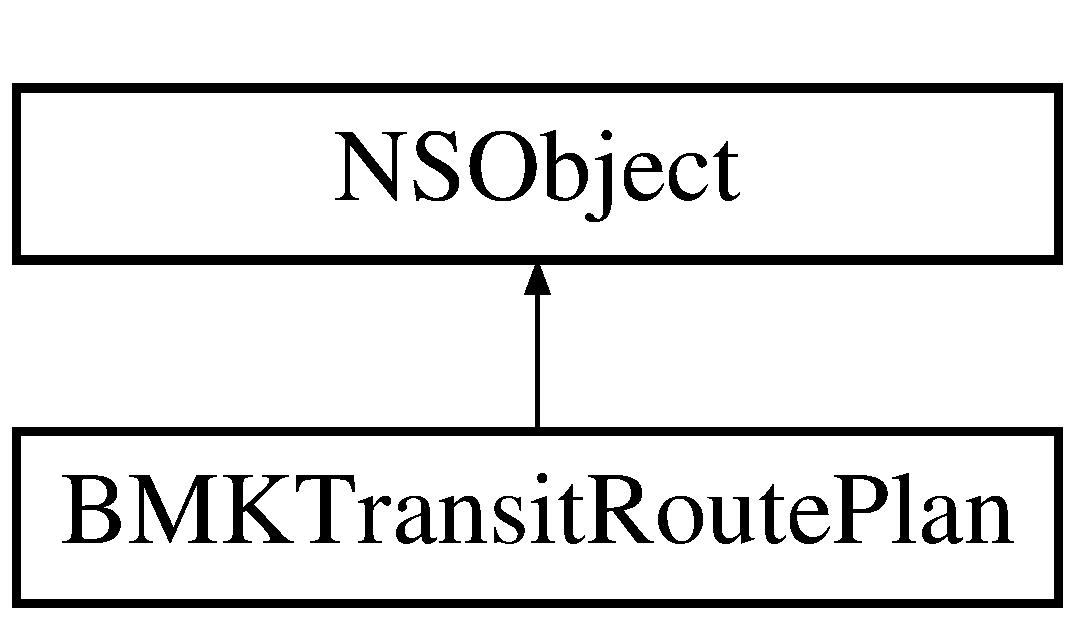
\includegraphics[height=2.000000cm]{interface_b_m_k_transit_route_plan}
\end{center}
\end{figure}
\subsection*{保护成员变量}
\begin{DoxyCompactItemize}
\item 
\hypertarget{interface_b_m_k_transit_route_plan_a60d824279339819c63dd3250e521e0c2}{int {\bfseries \-\_\-distance}}\label{interface_b_m_k_transit_route_plan_a60d824279339819c63dd3250e521e0c2}

\item 
\hypertarget{interface_b_m_k_transit_route_plan_a0c6a25bc877f5cb7be4031bcc3b41102}{N\-S\-String $\ast$ {\bfseries \-\_\-content}}\label{interface_b_m_k_transit_route_plan_a0c6a25bc877f5cb7be4031bcc3b41102}

\item 
\hypertarget{interface_b_m_k_transit_route_plan_abadaa366d74590f06156787fef1b66d0}{C\-L\-Location\-Coordinate2\-D {\bfseries \-\_\-start\-Pt}}\label{interface_b_m_k_transit_route_plan_abadaa366d74590f06156787fef1b66d0}

\item 
\hypertarget{interface_b_m_k_transit_route_plan_ad5a3329c1ea2831c13ec5aba78815504}{C\-L\-Location\-Coordinate2\-D {\bfseries \-\_\-end\-Pt}}\label{interface_b_m_k_transit_route_plan_ad5a3329c1ea2831c13ec5aba78815504}

\item 
\hypertarget{interface_b_m_k_transit_route_plan_a9353aa1b87321aad2492b57f801e3116}{N\-S\-Array $\ast$ {\bfseries \-\_\-routes}}\label{interface_b_m_k_transit_route_plan_a9353aa1b87321aad2492b57f801e3116}

\item 
\hypertarget{interface_b_m_k_transit_route_plan_aded38ebf485757a37633a026e503c999}{N\-S\-Array $\ast$ {\bfseries \-\_\-lines}}\label{interface_b_m_k_transit_route_plan_aded38ebf485757a37633a026e503c999}

\end{DoxyCompactItemize}
\subsection*{Properties}
\begin{DoxyCompactItemize}
\item 
\hypertarget{interface_b_m_k_transit_route_plan_a25d9fa314bf2c83d1d0503d7ac2ba6c8}{int \hyperlink{interface_b_m_k_transit_route_plan_a25d9fa314bf2c83d1d0503d7ac2ba6c8}{distance}}\label{interface_b_m_k_transit_route_plan_a25d9fa314bf2c83d1d0503d7ac2ba6c8}

\begin{DoxyCompactList}\small\item\em 线路距离,单位:米 \end{DoxyCompactList}\item 
\hypertarget{interface_b_m_k_transit_route_plan_a92851b16d2ec5bcd56bf937975470d1c}{C\-L\-Location\-Coordinate2\-D \hyperlink{interface_b_m_k_transit_route_plan_a92851b16d2ec5bcd56bf937975470d1c}{start\-Pt}}\label{interface_b_m_k_transit_route_plan_a92851b16d2ec5bcd56bf937975470d1c}

\begin{DoxyCompactList}\small\item\em 线路起点坐标 \end{DoxyCompactList}\item 
\hypertarget{interface_b_m_k_transit_route_plan_a29d6033e359e054ce3491822a58dacf5}{C\-L\-Location\-Coordinate2\-D \hyperlink{interface_b_m_k_transit_route_plan_a29d6033e359e054ce3491822a58dacf5}{end\-Pt}}\label{interface_b_m_k_transit_route_plan_a29d6033e359e054ce3491822a58dacf5}

\begin{DoxyCompactList}\small\item\em 线路终点坐标 \end{DoxyCompactList}\item 
\hypertarget{interface_b_m_k_transit_route_plan_a01cd9e49fac4e640816a065a8f774ae3}{N\-S\-String $\ast$ \hyperlink{interface_b_m_k_transit_route_plan_a01cd9e49fac4e640816a065a8f774ae3}{content}}\label{interface_b_m_k_transit_route_plan_a01cd9e49fac4e640816a065a8f774ae3}

\begin{DoxyCompactList}\small\item\em 方案描述信息 \end{DoxyCompactList}\item 
\hypertarget{interface_b_m_k_transit_route_plan_ab0071627e1da4ace544f5418fcffc114}{N\-S\-Array $\ast$ \hyperlink{interface_b_m_k_transit_route_plan_ab0071627e1da4ace544f5418fcffc114}{routes}}\label{interface_b_m_k_transit_route_plan_ab0071627e1da4ace544f5418fcffc114}

\begin{DoxyCompactList}\small\item\em B\-M\-K\-Route数组 \end{DoxyCompactList}\item 
\hypertarget{interface_b_m_k_transit_route_plan_a76eb4afd803434e6252318822c5df75e}{N\-S\-Array $\ast$ \hyperlink{interface_b_m_k_transit_route_plan_a76eb4afd803434e6252318822c5df75e}{lines}}\label{interface_b_m_k_transit_route_plan_a76eb4afd803434e6252318822c5df75e}

\begin{DoxyCompactList}\small\item\em B\-M\-K\-Line数组 \end{DoxyCompactList}\end{DoxyCompactItemize}


\subsection{详细描述}
公交方案详情类 

The documentation for this class was generated from the following file\-:\begin{DoxyCompactItemize}
\item 
B\-M\-K\-Route\-Search\-Type.\-h\end{DoxyCompactItemize}

\hypertarget{interface_b_m_k_user_location}{\section{B\-M\-K\-User\-Location 类参考}
\label{interface_b_m_k_user_location}\index{B\-M\-K\-User\-Location@{B\-M\-K\-User\-Location}}
}


定位信息类  




{\ttfamily \#import $<$B\-M\-K\-User\-Location.\-h$>$}

继承关系图 B\-M\-K\-User\-Location\-:\begin{figure}[H]
\begin{center}
\leavevmode
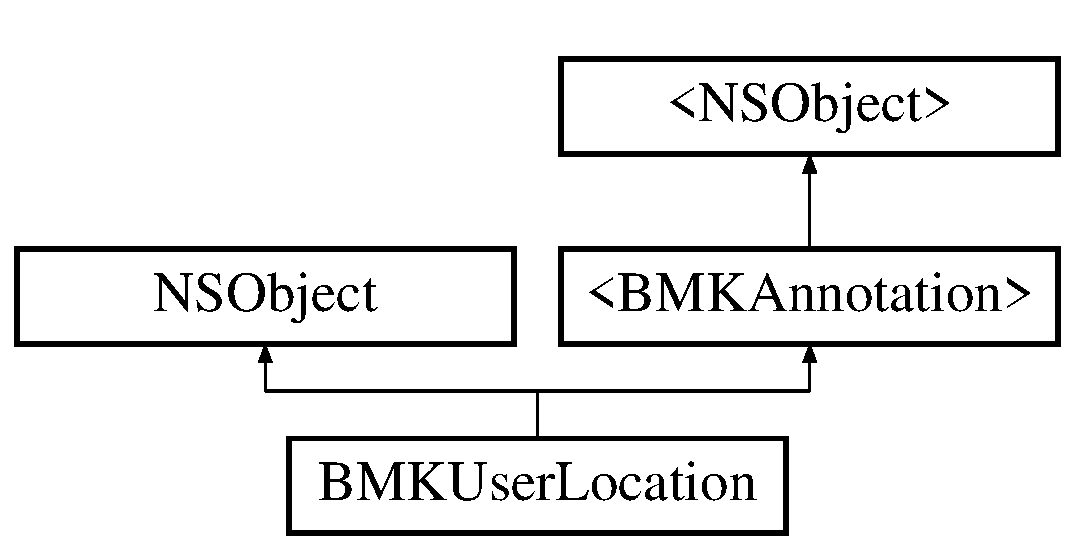
\includegraphics[height=3.000000cm]{interface_b_m_k_user_location}
\end{center}
\end{figure}
\subsection*{Properties}
\begin{DoxyCompactItemize}
\item 
\hypertarget{interface_b_m_k_user_location_a57e486ccb3b7665183e9e1eaa4d2716e}{B\-O\-O\-L \hyperlink{interface_b_m_k_user_location_a57e486ccb3b7665183e9e1eaa4d2716e}{updating}}\label{interface_b_m_k_user_location_a57e486ccb3b7665183e9e1eaa4d2716e}

\begin{DoxyCompactList}\small\item\em 位置更新状态,如果正在更新位置信息,则该值为\-Y\-E\-S \end{DoxyCompactList}\item 
\hypertarget{interface_b_m_k_user_location_aba4b76e55f4605c5554fe16aca1b4fbf}{C\-L\-Location $\ast$ \hyperlink{interface_b_m_k_user_location_aba4b76e55f4605c5554fe16aca1b4fbf}{location}}\label{interface_b_m_k_user_location_aba4b76e55f4605c5554fe16aca1b4fbf}

\begin{DoxyCompactList}\small\item\em 位置信息,如果\-B\-M\-K\-Map\-View的shows\-User\-Location为\-N\-O,或者尚未定位成功,则该值为nil \end{DoxyCompactList}\item 
\hypertarget{interface_b_m_k_user_location_a8fc42845ec226a1af2de73c8dd4d183d}{N\-S\-String $\ast$ \hyperlink{interface_b_m_k_user_location_a8fc42845ec226a1af2de73c8dd4d183d}{title}}\label{interface_b_m_k_user_location_a8fc42845ec226a1af2de73c8dd4d183d}

\begin{DoxyCompactList}\small\item\em 定位标注点要显示的标题信息 \end{DoxyCompactList}\item 
\hypertarget{interface_b_m_k_user_location_af38d7aa4f89637da255ca7308fcaa240}{N\-S\-String $\ast$ \hyperlink{interface_b_m_k_user_location_af38d7aa4f89637da255ca7308fcaa240}{subtitle}}\label{interface_b_m_k_user_location_af38d7aa4f89637da255ca7308fcaa240}

\begin{DoxyCompactList}\small\item\em 定位标注点要显示的子标题信息. \end{DoxyCompactList}\end{DoxyCompactItemize}
\subsection*{附加继承成员}


\subsection{详细描述}
定位信息类 

The documentation for this class was generated from the following file\-:\begin{DoxyCompactItemize}
\item 
B\-M\-K\-User\-Location.\-h\end{DoxyCompactItemize}

\chapter{File Documentation}
\hypertarget{_b_m_k_geometry_8h}{\section{B\-M\-K\-Geometry.\-h File Reference}
\label{_b_m_k_geometry_8h}\index{B\-M\-K\-Geometry.\-h@{B\-M\-K\-Geometry.\-h}}
}
{\ttfamily \#import $<$Core\-Graphics/\-Core\-Graphics.\-h$>$}\\*
{\ttfamily \#import $<$Core\-Location/\-Core\-Location.\-h$>$}\\*
{\ttfamily \#import $<$U\-I\-Kit/\-U\-I\-Kit.\-h$>$}\\*
\subsection*{类}
\begin{DoxyCompactItemize}
\item 
struct \hyperlink{struct_b_m_k_coordinate_span}{B\-M\-K\-Coordinate\-Span}
\begin{DoxyCompactList}\small\item\em 表示一个经纬度范围 \end{DoxyCompactList}\item 
struct \hyperlink{struct_b_m_k_coordinate_region}{B\-M\-K\-Coordinate\-Region}
\begin{DoxyCompactList}\small\item\em 表示一个经纬度区域 \end{DoxyCompactList}\item 
struct \hyperlink{struct_b_m_k_geo_point}{B\-M\-K\-Geo\-Point}
\begin{DoxyCompactList}\small\item\em 表示一个经纬度坐标点 \end{DoxyCompactList}\item 
struct \hyperlink{struct_b_m_k_map_point}{B\-M\-K\-Map\-Point}
\begin{DoxyCompactList}\small\item\em 地理坐标点,用直角地理坐标表示 \end{DoxyCompactList}\item 
struct \hyperlink{struct_b_m_k_map_size}{B\-M\-K\-Map\-Size}
\begin{DoxyCompactList}\small\item\em 矩形大小,用直角地理坐标表示 \end{DoxyCompactList}\item 
struct \hyperlink{struct_b_m_k_map_rect}{B\-M\-K\-Map\-Rect}
\begin{DoxyCompactList}\small\item\em 矩形,用直角地理坐标表示 \end{DoxyCompactList}\end{DoxyCompactItemize}
\subsection*{类型定义}
\begin{DoxyCompactItemize}
\item 
\hypertarget{_b_m_k_geometry_8h_abed0f3dd0db6f682408ae9a6593c7cc8}{typedef C\-G\-Float \hyperlink{_b_m_k_geometry_8h_abed0f3dd0db6f682408ae9a6593c7cc8}{B\-M\-K\-Zoom\-Scale}}\label{_b_m_k_geometry_8h_abed0f3dd0db6f682408ae9a6593c7cc8}

\begin{DoxyCompactList}\small\item\em 地图缩放比例 \end{DoxyCompactList}\end{DoxyCompactItemize}
\subsection*{方法}
\begin{DoxyCompactItemize}
\item 
U\-I\-K\-I\-T\-\_\-\-S\-T\-A\-T\-I\-C\-\_\-\-I\-N\-L\-I\-N\-E \\*
\hyperlink{struct_b_m_k_coordinate_span}{B\-M\-K\-Coordinate\-Span} \hyperlink{_b_m_k_geometry_8h_a252ea0a1948b9c7a595bd2b650aeae6d}{B\-M\-K\-Coordinate\-Span\-Make} (C\-L\-Location\-Degrees latitude\-Delta, C\-L\-Location\-Degrees longitude\-Delta)
\item 
U\-I\-K\-I\-T\-\_\-\-S\-T\-A\-T\-I\-C\-\_\-\-I\-N\-L\-I\-N\-E \\*
\hyperlink{struct_b_m_k_coordinate_region}{B\-M\-K\-Coordinate\-Region} \hyperlink{_b_m_k_geometry_8h_a4c055c14d6a80d14ada771f062916394}{B\-M\-K\-Coordinate\-Region\-Make} (C\-L\-Location\-Coordinate2\-D center\-Coordinate, \hyperlink{struct_b_m_k_coordinate_span}{B\-M\-K\-Coordinate\-Span} span)
\item 
U\-I\-K\-I\-T\-\_\-\-E\-X\-T\-E\-R\-N \hyperlink{struct_b_m_k_coordinate_region}{B\-M\-K\-Coordinate\-Region} \hyperlink{_b_m_k_geometry_8h_a30878e885fa02a2605bb194645736a36}{B\-M\-K\-Coordinate\-Region\-Make\-With\-Distance} (C\-L\-Location\-Coordinate2\-D center\-Coordinate, C\-L\-Location\-Distance latitudinal\-Meters, C\-L\-Location\-Distance longitudinal\-Meters)
\item 
U\-I\-K\-I\-T\-\_\-\-E\-X\-T\-E\-R\-N \hyperlink{struct_b_m_k_map_point}{B\-M\-K\-Map\-Point} \hyperlink{_b_m_k_geometry_8h_a8cdb8447bff118ee28d8de511faf32a7}{B\-M\-K\-Map\-Point\-For\-Coordinate} (C\-L\-Location\-Coordinate2\-D coordinate)
\item 
U\-I\-K\-I\-T\-\_\-\-E\-X\-T\-E\-R\-N C\-L\-Location\-Coordinate2\-D \hyperlink{_b_m_k_geometry_8h_a82e1819974df12b83c0f899b27f1e1cd}{B\-M\-K\-Coordinate\-For\-Map\-Point} (\hyperlink{struct_b_m_k_map_point}{B\-M\-K\-Map\-Point} map\-Point)
\item 
U\-I\-K\-I\-T\-\_\-\-E\-X\-T\-E\-R\-N C\-L\-Location\-Distance \hyperlink{_b_m_k_geometry_8h_acd9d69e5e899ef5acad884002c83eda5}{B\-M\-K\-Meters\-Per\-Map\-Point\-At\-Latitude} (C\-L\-Location\-Degrees latitude)
\item 
U\-I\-K\-I\-T\-\_\-\-E\-X\-T\-E\-R\-N double \hyperlink{_b_m_k_geometry_8h_a3766563510b0551c4304fa06562e54a2}{B\-M\-K\-Map\-Points\-Per\-Meter\-At\-Latitude} (C\-L\-Location\-Degrees latitude)
\item 
U\-I\-K\-I\-T\-\_\-\-E\-X\-T\-E\-R\-N C\-L\-Location\-Distance \hyperlink{_b_m_k_geometry_8h_a6051f3027c1960e53101fa95357ce068}{B\-M\-K\-Meters\-Between\-Map\-Points} (\hyperlink{struct_b_m_k_map_point}{B\-M\-K\-Map\-Point} a, \hyperlink{struct_b_m_k_map_point}{B\-M\-K\-Map\-Point} b)
\item 
U\-I\-K\-I\-T\-\_\-\-S\-T\-A\-T\-I\-C\-\_\-\-I\-N\-L\-I\-N\-E \hyperlink{struct_b_m_k_map_point}{B\-M\-K\-Map\-Point} \hyperlink{_b_m_k_geometry_8h_a1afb640d3e67cb96e0f5e0cf878becee}{B\-M\-K\-Map\-Point\-Make} (double x, double y)
\item 
U\-I\-K\-I\-T\-\_\-\-S\-T\-A\-T\-I\-C\-\_\-\-I\-N\-L\-I\-N\-E \hyperlink{struct_b_m_k_map_size}{B\-M\-K\-Map\-Size} \hyperlink{_b_m_k_geometry_8h_afc821309dd42822252fb54c1fa484bd8}{B\-M\-K\-Map\-Size\-Make} (double width, double height)
\item 
U\-I\-K\-I\-T\-\_\-\-S\-T\-A\-T\-I\-C\-\_\-\-I\-N\-L\-I\-N\-E \hyperlink{struct_b_m_k_map_rect}{B\-M\-K\-Map\-Rect} \hyperlink{_b_m_k_geometry_8h_ae36b2f884d73d7e119bb224b33e70eff}{B\-M\-K\-Map\-Rect\-Make} (double x, double y, double width, double height)
\item 
U\-I\-K\-I\-T\-\_\-\-S\-T\-A\-T\-I\-C\-\_\-\-I\-N\-L\-I\-N\-E double \hyperlink{_b_m_k_geometry_8h_a294cad295bdd1f4108e18993b425eb87}{B\-M\-K\-Map\-Rect\-Get\-Min\-X} (\hyperlink{struct_b_m_k_map_rect}{B\-M\-K\-Map\-Rect} rect)
\item 
U\-I\-K\-I\-T\-\_\-\-S\-T\-A\-T\-I\-C\-\_\-\-I\-N\-L\-I\-N\-E double \hyperlink{_b_m_k_geometry_8h_a45df48e78b212b924723cb16f8b68e24}{B\-M\-K\-Map\-Rect\-Get\-Min\-Y} (\hyperlink{struct_b_m_k_map_rect}{B\-M\-K\-Map\-Rect} rect)
\item 
U\-I\-K\-I\-T\-\_\-\-S\-T\-A\-T\-I\-C\-\_\-\-I\-N\-L\-I\-N\-E double \hyperlink{_b_m_k_geometry_8h_ae0dfe0ab0cdde7d492e408f564fe9358}{B\-M\-K\-Map\-Rect\-Get\-Mid\-X} (\hyperlink{struct_b_m_k_map_rect}{B\-M\-K\-Map\-Rect} rect)
\item 
U\-I\-K\-I\-T\-\_\-\-S\-T\-A\-T\-I\-C\-\_\-\-I\-N\-L\-I\-N\-E double \hyperlink{_b_m_k_geometry_8h_ac5c23791f6c1eaddc2d625b059c88c54}{B\-M\-K\-Map\-Rect\-Get\-Mid\-Y} (\hyperlink{struct_b_m_k_map_rect}{B\-M\-K\-Map\-Rect} rect)
\item 
U\-I\-K\-I\-T\-\_\-\-S\-T\-A\-T\-I\-C\-\_\-\-I\-N\-L\-I\-N\-E double \hyperlink{_b_m_k_geometry_8h_a4e30d4345cd56ca13f6e882836ffa9ce}{B\-M\-K\-Map\-Rect\-Get\-Max\-X} (\hyperlink{struct_b_m_k_map_rect}{B\-M\-K\-Map\-Rect} rect)
\item 
U\-I\-K\-I\-T\-\_\-\-S\-T\-A\-T\-I\-C\-\_\-\-I\-N\-L\-I\-N\-E double \hyperlink{_b_m_k_geometry_8h_ac8d52fde1866ea9c3d19c33371c5c0d8}{B\-M\-K\-Map\-Rect\-Get\-Max\-Y} (\hyperlink{struct_b_m_k_map_rect}{B\-M\-K\-Map\-Rect} rect)
\item 
U\-I\-K\-I\-T\-\_\-\-S\-T\-A\-T\-I\-C\-\_\-\-I\-N\-L\-I\-N\-E double \hyperlink{_b_m_k_geometry_8h_a2c1a5ec9570711e8524827fa9a395d0d}{B\-M\-K\-Map\-Rect\-Get\-Width} (\hyperlink{struct_b_m_k_map_rect}{B\-M\-K\-Map\-Rect} rect)
\item 
U\-I\-K\-I\-T\-\_\-\-S\-T\-A\-T\-I\-C\-\_\-\-I\-N\-L\-I\-N\-E double \hyperlink{_b_m_k_geometry_8h_ab5ea9c49c319a9ae494a7da167be6189}{B\-M\-K\-Map\-Rect\-Get\-Height} (\hyperlink{struct_b_m_k_map_rect}{B\-M\-K\-Map\-Rect} rect)
\item 
U\-I\-K\-I\-T\-\_\-\-S\-T\-A\-T\-I\-C\-\_\-\-I\-N\-L\-I\-N\-E B\-O\-O\-L \hyperlink{_b_m_k_geometry_8h_ade1aa48d7c452c6aae008fe2890fe05b}{B\-M\-K\-Map\-Point\-Equal\-To\-Point} (\hyperlink{struct_b_m_k_map_point}{B\-M\-K\-Map\-Point} point1, \hyperlink{struct_b_m_k_map_point}{B\-M\-K\-Map\-Point} point2)
\item 
U\-I\-K\-I\-T\-\_\-\-S\-T\-A\-T\-I\-C\-\_\-\-I\-N\-L\-I\-N\-E B\-O\-O\-L \hyperlink{_b_m_k_geometry_8h_adc307cf3a5707b82e78265ba6be1ffc4}{B\-M\-K\-Map\-Size\-Equal\-To\-Size} (\hyperlink{struct_b_m_k_map_size}{B\-M\-K\-Map\-Size} size1, \hyperlink{struct_b_m_k_map_size}{B\-M\-K\-Map\-Size} size2)
\item 
U\-I\-K\-I\-T\-\_\-\-S\-T\-A\-T\-I\-C\-\_\-\-I\-N\-L\-I\-N\-E B\-O\-O\-L \hyperlink{_b_m_k_geometry_8h_aa64e3dd2b0333ddadda311abb367fc39}{B\-M\-K\-Map\-Rect\-Equal\-To\-Rect} (\hyperlink{struct_b_m_k_map_rect}{B\-M\-K\-Map\-Rect} rect1, \hyperlink{struct_b_m_k_map_rect}{B\-M\-K\-Map\-Rect} rect2)
\item 
U\-I\-K\-I\-T\-\_\-\-S\-T\-A\-T\-I\-C\-\_\-\-I\-N\-L\-I\-N\-E B\-O\-O\-L \hyperlink{_b_m_k_geometry_8h_a2abc95ac03215aad58b7a02f54264605}{B\-M\-K\-Map\-Rect\-Is\-Null} (\hyperlink{struct_b_m_k_map_rect}{B\-M\-K\-Map\-Rect} rect)
\item 
U\-I\-K\-I\-T\-\_\-\-S\-T\-A\-T\-I\-C\-\_\-\-I\-N\-L\-I\-N\-E B\-O\-O\-L \hyperlink{_b_m_k_geometry_8h_a6a49884fe83e2aeb08b6827bf9361ef9}{B\-M\-K\-Map\-Rect\-Is\-Empty} (\hyperlink{struct_b_m_k_map_rect}{B\-M\-K\-Map\-Rect} rect)
\item 
U\-I\-K\-I\-T\-\_\-\-S\-T\-A\-T\-I\-C\-\_\-\-I\-N\-L\-I\-N\-E N\-S\-String $\ast$ \hyperlink{_b_m_k_geometry_8h_a6f2b502558d61983e911e77b02f86166}{B\-M\-K\-String\-From\-Map\-Point} (\hyperlink{struct_b_m_k_map_point}{B\-M\-K\-Map\-Point} point)
\item 
U\-I\-K\-I\-T\-\_\-\-S\-T\-A\-T\-I\-C\-\_\-\-I\-N\-L\-I\-N\-E N\-S\-String $\ast$ \hyperlink{_b_m_k_geometry_8h_a687e957bfdaee6c3e7ef97c3831127d2}{B\-M\-K\-String\-From\-Map\-Size} (\hyperlink{struct_b_m_k_map_size}{B\-M\-K\-Map\-Size} size)
\item 
U\-I\-K\-I\-T\-\_\-\-S\-T\-A\-T\-I\-C\-\_\-\-I\-N\-L\-I\-N\-E N\-S\-String $\ast$ \hyperlink{_b_m_k_geometry_8h_a07c0dc35e145b24828d11e20e8d1456e}{B\-M\-K\-String\-From\-Map\-Rect} (\hyperlink{struct_b_m_k_map_rect}{B\-M\-K\-Map\-Rect} rect)
\item 
U\-I\-K\-I\-T\-\_\-\-E\-X\-T\-E\-R\-N \hyperlink{struct_b_m_k_map_rect}{B\-M\-K\-Map\-Rect} \hyperlink{_b_m_k_geometry_8h_aca2a7535ee5bfbd1204f48d2536f11ba}{B\-M\-K\-Map\-Rect\-Union} (\hyperlink{struct_b_m_k_map_rect}{B\-M\-K\-Map\-Rect} rect1, \hyperlink{struct_b_m_k_map_rect}{B\-M\-K\-Map\-Rect} rect2)
\item 
U\-I\-K\-I\-T\-\_\-\-E\-X\-T\-E\-R\-N \hyperlink{struct_b_m_k_map_rect}{B\-M\-K\-Map\-Rect} \hyperlink{_b_m_k_geometry_8h_af46516f57d0abfd6d8aa902bc50060a6}{B\-M\-K\-Map\-Rect\-Intersection} (\hyperlink{struct_b_m_k_map_rect}{B\-M\-K\-Map\-Rect} rect1, \hyperlink{struct_b_m_k_map_rect}{B\-M\-K\-Map\-Rect} rect2)
\item 
U\-I\-K\-I\-T\-\_\-\-E\-X\-T\-E\-R\-N \hyperlink{struct_b_m_k_map_rect}{B\-M\-K\-Map\-Rect} \hyperlink{_b_m_k_geometry_8h_a717e60a9798195b716d083f3e8da1d54}{B\-M\-K\-Map\-Rect\-Inset} (\hyperlink{struct_b_m_k_map_rect}{B\-M\-K\-Map\-Rect} rect, double dx, double dy)
\item 
U\-I\-K\-I\-T\-\_\-\-E\-X\-T\-E\-R\-N \hyperlink{struct_b_m_k_map_rect}{B\-M\-K\-Map\-Rect} \hyperlink{_b_m_k_geometry_8h_a895de18577c2de7a4d0843d61be5d948}{B\-M\-K\-Map\-Rect\-Offset} (\hyperlink{struct_b_m_k_map_rect}{B\-M\-K\-Map\-Rect} rect, double dx, double dy)
\item 
U\-I\-K\-I\-T\-\_\-\-E\-X\-T\-E\-R\-N void \hyperlink{_b_m_k_geometry_8h_a32fb4cbbc882aefdffb1981b2a445621}{B\-M\-K\-Map\-Rect\-Divide} (\hyperlink{struct_b_m_k_map_rect}{B\-M\-K\-Map\-Rect} rect, \hyperlink{struct_b_m_k_map_rect}{B\-M\-K\-Map\-Rect} $\ast$slice, \hyperlink{struct_b_m_k_map_rect}{B\-M\-K\-Map\-Rect} $\ast$remainder, double amount, C\-G\-Rect\-Edge edge)
\item 
U\-I\-K\-I\-T\-\_\-\-E\-X\-T\-E\-R\-N B\-O\-O\-L \hyperlink{_b_m_k_geometry_8h_a756802dc5d51b9e783f9d83711b2972f}{B\-M\-K\-Map\-Rect\-Contains\-Point} (\hyperlink{struct_b_m_k_map_rect}{B\-M\-K\-Map\-Rect} rect, \hyperlink{struct_b_m_k_map_point}{B\-M\-K\-Map\-Point} point)
\item 
U\-I\-K\-I\-T\-\_\-\-E\-X\-T\-E\-R\-N B\-O\-O\-L \hyperlink{_b_m_k_geometry_8h_a3bf9df0b02a9c78e5daa7862c3c197e5}{B\-M\-K\-Map\-Rect\-Contains\-Rect} (\hyperlink{struct_b_m_k_map_rect}{B\-M\-K\-Map\-Rect} rect1, \hyperlink{struct_b_m_k_map_rect}{B\-M\-K\-Map\-Rect} rect2)
\item 
U\-I\-K\-I\-T\-\_\-\-E\-X\-T\-E\-R\-N B\-O\-O\-L \hyperlink{_b_m_k_geometry_8h_ad8fc8d14cda123242c551db6c820e0a1}{B\-M\-K\-Map\-Rect\-Intersects\-Rect} (\hyperlink{struct_b_m_k_map_rect}{B\-M\-K\-Map\-Rect} rect1, \hyperlink{struct_b_m_k_map_rect}{B\-M\-K\-Map\-Rect} rect2)
\item 
U\-I\-K\-I\-T\-\_\-\-E\-X\-T\-E\-R\-N \hyperlink{struct_b_m_k_coordinate_region}{B\-M\-K\-Coordinate\-Region} \hyperlink{_b_m_k_geometry_8h_a779ad65709d575145d839d1d7e972064}{B\-M\-K\-Coordinate\-Region\-For\-Map\-Rect} (\hyperlink{struct_b_m_k_map_rect}{B\-M\-K\-Map\-Rect} rect)
\item 
U\-I\-K\-I\-T\-\_\-\-E\-X\-T\-E\-R\-N B\-O\-O\-L \hyperlink{_b_m_k_geometry_8h_a2fa044766e6c2c56e831a552c1b25d7b}{B\-M\-K\-Map\-Rect\-Spans180th\-Meridian} (\hyperlink{struct_b_m_k_map_rect}{B\-M\-K\-Map\-Rect} rect)
\item 
U\-I\-K\-I\-T\-\_\-\-E\-X\-T\-E\-R\-N \hyperlink{struct_b_m_k_map_rect}{B\-M\-K\-Map\-Rect} \hyperlink{_b_m_k_geometry_8h_acdf6820a550a4c953020fc136a17e4b1}{B\-M\-K\-Map\-Rect\-Remainder} (\hyperlink{struct_b_m_k_map_rect}{B\-M\-K\-Map\-Rect} rect)
\item 
U\-I\-K\-I\-T\-\_\-\-E\-X\-T\-E\-R\-N N\-S\-Dictionary $\ast$ \hyperlink{_b_m_k_geometry_8h_ac0042bf0c14fb602653c632fe0744bca}{B\-M\-K\-Baidu\-Coor\-For\-Wgs84} (C\-L\-Location\-Coordinate2\-D coor\-Wgs84)
\item 
U\-I\-K\-I\-T\-\_\-\-E\-X\-T\-E\-R\-N N\-S\-Dictionary $\ast$ \hyperlink{_b_m_k_geometry_8h_abb548b27e546ef88ad8d8a6aef9912fc}{B\-M\-K\-Baidu\-Coor\-For\-Gcj} (C\-L\-Location\-Coordinate2\-D coor\-Gcj)
\item 
U\-I\-K\-I\-T\-\_\-\-E\-X\-T\-E\-R\-N C\-L\-Location\-Coordinate2\-D \hyperlink{_b_m_k_geometry_8h_ac75142905f8c4cd5e3bf63e2b01f5b06}{B\-M\-K\-Coor\-Dictionary\-Decode} (N\-S\-Dictionary $\ast$dictionary)
\end{DoxyCompactItemize}
\subsection*{变量}
\begin{DoxyCompactItemize}
\item 
\hypertarget{_b_m_k_geometry_8h_ac9bf7216ae963df0e287280d418fa514}{U\-I\-K\-I\-T\-\_\-\-E\-X\-T\-E\-R\-N const \hyperlink{struct_b_m_k_map_size}{B\-M\-K\-Map\-Size} \hyperlink{_b_m_k_geometry_8h_ac9bf7216ae963df0e287280d418fa514}{B\-M\-K\-Map\-Size\-World}}\label{_b_m_k_geometry_8h_ac9bf7216ae963df0e287280d418fa514}

\begin{DoxyCompactList}\small\item\em 经过投影后的世界范围大小,与经纬度(-\/85,180)投影后的坐标值对应 \end{DoxyCompactList}\item 
\hypertarget{_b_m_k_geometry_8h_a9b78f5781da65e22ac697e10716653f7}{U\-I\-K\-I\-T\-\_\-\-E\-X\-T\-E\-R\-N const \hyperlink{struct_b_m_k_map_rect}{B\-M\-K\-Map\-Rect} \hyperlink{_b_m_k_geometry_8h_a9b78f5781da65e22ac697e10716653f7}{B\-M\-K\-Map\-Rect\-World}}\label{_b_m_k_geometry_8h_a9b78f5781da65e22ac697e10716653f7}

\begin{DoxyCompactList}\small\item\em 经过投影后的世界矩形范围 \end{DoxyCompactList}\item 
\hypertarget{_b_m_k_geometry_8h_ac7981ded0b24ec5028a079760e207698}{U\-I\-K\-I\-T\-\_\-\-E\-X\-T\-E\-R\-N const \hyperlink{struct_b_m_k_map_rect}{B\-M\-K\-Map\-Rect} \hyperlink{_b_m_k_geometry_8h_ac7981ded0b24ec5028a079760e207698}{B\-M\-K\-Map\-Rect\-Null}}\label{_b_m_k_geometry_8h_ac7981ded0b24ec5028a079760e207698}

\begin{DoxyCompactList}\small\item\em 空的直角坐标矩形 \end{DoxyCompactList}\end{DoxyCompactItemize}


\subsection{详细描述}
B\-Map\-Kit

Copyright 2011 Baidu Inc. All rights reserved. 

\subsection{Function Documentation}
\hypertarget{_b_m_k_geometry_8h_abb548b27e546ef88ad8d8a6aef9912fc}{\index{B\-M\-K\-Geometry.\-h@{B\-M\-K\-Geometry.\-h}!B\-M\-K\-Baidu\-Coor\-For\-Gcj@{B\-M\-K\-Baidu\-Coor\-For\-Gcj}}
\index{B\-M\-K\-Baidu\-Coor\-For\-Gcj@{B\-M\-K\-Baidu\-Coor\-For\-Gcj}!BMKGeometry.h@{B\-M\-K\-Geometry.\-h}}
\subsubsection[{B\-M\-K\-Baidu\-Coor\-For\-Gcj}]{\setlength{\rightskip}{0pt plus 5cm}U\-I\-K\-I\-T\-\_\-\-E\-X\-T\-E\-R\-N N\-S\-Dictionary$\ast$ B\-M\-K\-Baidu\-Coor\-For\-Gcj (
\begin{DoxyParamCaption}
\item[{C\-L\-Location\-Coordinate2\-D}]{coor\-Gcj}
\end{DoxyParamCaption}
)}}\label{_b_m_k_geometry_8h_abb548b27e546ef88ad8d8a6aef9912fc}
坐标转换函数,从google坐标,51地图坐标,mapabc坐标转换为百度坐标(51地图坐标需要显出10000) 
\begin{DoxyParams}{参数}
{\em coor\-Gcj} & 待转换的google坐标,51地图坐标,mapabc坐标 \\
\hline
\end{DoxyParams}
\begin{DoxyReturn}{返回}
返回的\-N\-S\-Dictionry中包含“x”,“y”字段,各自对应经过base64加密之后的x,y坐标 
\end{DoxyReturn}
\hypertarget{_b_m_k_geometry_8h_ac0042bf0c14fb602653c632fe0744bca}{\index{B\-M\-K\-Geometry.\-h@{B\-M\-K\-Geometry.\-h}!B\-M\-K\-Baidu\-Coor\-For\-Wgs84@{B\-M\-K\-Baidu\-Coor\-For\-Wgs84}}
\index{B\-M\-K\-Baidu\-Coor\-For\-Wgs84@{B\-M\-K\-Baidu\-Coor\-For\-Wgs84}!BMKGeometry.h@{B\-M\-K\-Geometry.\-h}}
\subsubsection[{B\-M\-K\-Baidu\-Coor\-For\-Wgs84}]{\setlength{\rightskip}{0pt plus 5cm}U\-I\-K\-I\-T\-\_\-\-E\-X\-T\-E\-R\-N N\-S\-Dictionary$\ast$ B\-M\-K\-Baidu\-Coor\-For\-Wgs84 (
\begin{DoxyParamCaption}
\item[{C\-L\-Location\-Coordinate2\-D}]{coor\-Wgs84}
\end{DoxyParamCaption}
)}}\label{_b_m_k_geometry_8h_ac0042bf0c14fb602653c632fe0744bca}
坐标转换函数,从原始\-G\-P\-S坐标,mapbar坐标转换成百度坐标 
\begin{DoxyParams}{参数}
{\em coor\-Wgs84} & 待转换的原始\-G\-P\-S坐标,或者mapbar的坐标 \\
\hline
\end{DoxyParams}
\begin{DoxyReturn}{返回}
返回的\-N\-S\-Dictionry中包含“x”,“y”字段,各自对应经过base64加密之后的x,y坐标 
\end{DoxyReturn}
\hypertarget{_b_m_k_geometry_8h_ac75142905f8c4cd5e3bf63e2b01f5b06}{\index{B\-M\-K\-Geometry.\-h@{B\-M\-K\-Geometry.\-h}!B\-M\-K\-Coor\-Dictionary\-Decode@{B\-M\-K\-Coor\-Dictionary\-Decode}}
\index{B\-M\-K\-Coor\-Dictionary\-Decode@{B\-M\-K\-Coor\-Dictionary\-Decode}!BMKGeometry.h@{B\-M\-K\-Geometry.\-h}}
\subsubsection[{B\-M\-K\-Coor\-Dictionary\-Decode}]{\setlength{\rightskip}{0pt plus 5cm}U\-I\-K\-I\-T\-\_\-\-E\-X\-T\-E\-R\-N C\-L\-Location\-Coordinate2\-D B\-M\-K\-Coor\-Dictionary\-Decode (
\begin{DoxyParamCaption}
\item[{N\-S\-Dictionary $\ast$}]{dictionary}
\end{DoxyParamCaption}
)}}\label{_b_m_k_geometry_8h_ac75142905f8c4cd5e3bf63e2b01f5b06}
base64加密后的坐标字典解密函数 
\begin{DoxyParams}{参数}
{\em dictionary} & 带解密的\-N\-S\-Dictionry,该\-N\-S\-Dictionry中应包含“x”,“y”字段,各自对应经过base64加密之后的x,y坐标 \\
\hline
\end{DoxyParams}
\begin{DoxyReturn}{返回}
解密之后的坐标 
\end{DoxyReturn}
\hypertarget{_b_m_k_geometry_8h_a82e1819974df12b83c0f899b27f1e1cd}{\index{B\-M\-K\-Geometry.\-h@{B\-M\-K\-Geometry.\-h}!B\-M\-K\-Coordinate\-For\-Map\-Point@{B\-M\-K\-Coordinate\-For\-Map\-Point}}
\index{B\-M\-K\-Coordinate\-For\-Map\-Point@{B\-M\-K\-Coordinate\-For\-Map\-Point}!BMKGeometry.h@{B\-M\-K\-Geometry.\-h}}
\subsubsection[{B\-M\-K\-Coordinate\-For\-Map\-Point}]{\setlength{\rightskip}{0pt plus 5cm}U\-I\-K\-I\-T\-\_\-\-E\-X\-T\-E\-R\-N C\-L\-Location\-Coordinate2\-D B\-M\-K\-Coordinate\-For\-Map\-Point (
\begin{DoxyParamCaption}
\item[{{\bf B\-M\-K\-Map\-Point}}]{map\-Point}
\end{DoxyParamCaption}
)}}\label{_b_m_k_geometry_8h_a82e1819974df12b83c0f899b27f1e1cd}
将投影后的直角地理坐标转换为经纬度坐标 
\begin{DoxyParams}{参数}
{\em map\-Point} & 投影后的直角地理坐标 \\
\hline
\end{DoxyParams}
\begin{DoxyReturn}{返回}
转换后的经纬度坐标 
\end{DoxyReturn}
\hypertarget{_b_m_k_geometry_8h_a779ad65709d575145d839d1d7e972064}{\index{B\-M\-K\-Geometry.\-h@{B\-M\-K\-Geometry.\-h}!B\-M\-K\-Coordinate\-Region\-For\-Map\-Rect@{B\-M\-K\-Coordinate\-Region\-For\-Map\-Rect}}
\index{B\-M\-K\-Coordinate\-Region\-For\-Map\-Rect@{B\-M\-K\-Coordinate\-Region\-For\-Map\-Rect}!BMKGeometry.h@{B\-M\-K\-Geometry.\-h}}
\subsubsection[{B\-M\-K\-Coordinate\-Region\-For\-Map\-Rect}]{\setlength{\rightskip}{0pt plus 5cm}U\-I\-K\-I\-T\-\_\-\-E\-X\-T\-E\-R\-N {\bf B\-M\-K\-Coordinate\-Region} B\-M\-K\-Coordinate\-Region\-For\-Map\-Rect (
\begin{DoxyParamCaption}
\item[{{\bf B\-M\-K\-Map\-Rect}}]{rect}
\end{DoxyParamCaption}
)}}\label{_b_m_k_geometry_8h_a779ad65709d575145d839d1d7e972064}
将投影后的直角坐标矩形转换为泳经纬度表示的范围 
\begin{DoxyParams}{参数}
{\em rect} & 待转换的直角坐标矩形 \\
\hline
\end{DoxyParams}
\begin{DoxyReturn}{返回}
转换后的经纬度范围 
\end{DoxyReturn}
\hypertarget{_b_m_k_geometry_8h_a4c055c14d6a80d14ada771f062916394}{\index{B\-M\-K\-Geometry.\-h@{B\-M\-K\-Geometry.\-h}!B\-M\-K\-Coordinate\-Region\-Make@{B\-M\-K\-Coordinate\-Region\-Make}}
\index{B\-M\-K\-Coordinate\-Region\-Make@{B\-M\-K\-Coordinate\-Region\-Make}!BMKGeometry.h@{B\-M\-K\-Geometry.\-h}}
\subsubsection[{B\-M\-K\-Coordinate\-Region\-Make}]{\setlength{\rightskip}{0pt plus 5cm}U\-I\-K\-I\-T\-\_\-\-S\-T\-A\-T\-I\-C\-\_\-\-I\-N\-L\-I\-N\-E {\bf B\-M\-K\-Coordinate\-Region} B\-M\-K\-Coordinate\-Region\-Make (
\begin{DoxyParamCaption}
\item[{C\-L\-Location\-Coordinate2\-D}]{center\-Coordinate, }
\item[{{\bf B\-M\-K\-Coordinate\-Span}}]{span}
\end{DoxyParamCaption}
)}}\label{_b_m_k_geometry_8h_a4c055c14d6a80d14ada771f062916394}
构造\-B\-M\-K\-Coordinate\-Region对象 
\begin{DoxyParams}{参数}
{\em center\-Coordinate} & 中心点经纬度坐标 \\
\hline
{\em span} & 经纬度的范围 \\
\hline
\end{DoxyParams}
\begin{DoxyReturn}{返回}
根据指定参数生成的\-B\-M\-K\-Coordinate\-Region对象 
\end{DoxyReturn}
\hypertarget{_b_m_k_geometry_8h_a30878e885fa02a2605bb194645736a36}{\index{B\-M\-K\-Geometry.\-h@{B\-M\-K\-Geometry.\-h}!B\-M\-K\-Coordinate\-Region\-Make\-With\-Distance@{B\-M\-K\-Coordinate\-Region\-Make\-With\-Distance}}
\index{B\-M\-K\-Coordinate\-Region\-Make\-With\-Distance@{B\-M\-K\-Coordinate\-Region\-Make\-With\-Distance}!BMKGeometry.h@{B\-M\-K\-Geometry.\-h}}
\subsubsection[{B\-M\-K\-Coordinate\-Region\-Make\-With\-Distance}]{\setlength{\rightskip}{0pt plus 5cm}U\-I\-K\-I\-T\-\_\-\-E\-X\-T\-E\-R\-N {\bf B\-M\-K\-Coordinate\-Region} B\-M\-K\-Coordinate\-Region\-Make\-With\-Distance (
\begin{DoxyParamCaption}
\item[{C\-L\-Location\-Coordinate2\-D}]{center\-Coordinate, }
\item[{C\-L\-Location\-Distance}]{latitudinal\-Meters, }
\item[{C\-L\-Location\-Distance}]{longitudinal\-Meters}
\end{DoxyParamCaption}
)}}\label{_b_m_k_geometry_8h_a30878e885fa02a2605bb194645736a36}
根据中心点和距离生成\-B\-M\-K\-Coordinate\-Region 
\begin{DoxyParams}{参数}
{\em center\-Coordinate} & 中心点坐标 \\
\hline
{\em latitudinal\-Meters} & 纬度方向的距离范围,单位:米 \\
\hline
{\em longitudinal\-Meters} & 经度方向的距离范围,单位:米 \\
\hline
\end{DoxyParams}
\begin{DoxyReturn}{返回}
根据中心点和距离生成\-B\-M\-K\-Coordinate\-Region 
\end{DoxyReturn}
\hypertarget{_b_m_k_geometry_8h_a252ea0a1948b9c7a595bd2b650aeae6d}{\index{B\-M\-K\-Geometry.\-h@{B\-M\-K\-Geometry.\-h}!B\-M\-K\-Coordinate\-Span\-Make@{B\-M\-K\-Coordinate\-Span\-Make}}
\index{B\-M\-K\-Coordinate\-Span\-Make@{B\-M\-K\-Coordinate\-Span\-Make}!BMKGeometry.h@{B\-M\-K\-Geometry.\-h}}
\subsubsection[{B\-M\-K\-Coordinate\-Span\-Make}]{\setlength{\rightskip}{0pt plus 5cm}U\-I\-K\-I\-T\-\_\-\-S\-T\-A\-T\-I\-C\-\_\-\-I\-N\-L\-I\-N\-E {\bf B\-M\-K\-Coordinate\-Span} B\-M\-K\-Coordinate\-Span\-Make (
\begin{DoxyParamCaption}
\item[{C\-L\-Location\-Degrees}]{latitude\-Delta, }
\item[{C\-L\-Location\-Degrees}]{longitude\-Delta}
\end{DoxyParamCaption}
)}}\label{_b_m_k_geometry_8h_a252ea0a1948b9c7a595bd2b650aeae6d}
构造\-B\-M\-K\-Coordinate\-Span对象 
\begin{DoxyParams}{参数}
{\em latitude\-Delta} & 纬度方向的变化量 \\
\hline
{\em longitude\-Delta} & 经度方向的变化量 \\
\hline
\end{DoxyParams}
\begin{DoxyReturn}{返回}
根据指定参数生成的\-B\-M\-K\-Coordinate\-Span对象 
\end{DoxyReturn}
\hypertarget{_b_m_k_geometry_8h_ade1aa48d7c452c6aae008fe2890fe05b}{\index{B\-M\-K\-Geometry.\-h@{B\-M\-K\-Geometry.\-h}!B\-M\-K\-Map\-Point\-Equal\-To\-Point@{B\-M\-K\-Map\-Point\-Equal\-To\-Point}}
\index{B\-M\-K\-Map\-Point\-Equal\-To\-Point@{B\-M\-K\-Map\-Point\-Equal\-To\-Point}!BMKGeometry.h@{B\-M\-K\-Geometry.\-h}}
\subsubsection[{B\-M\-K\-Map\-Point\-Equal\-To\-Point}]{\setlength{\rightskip}{0pt plus 5cm}U\-I\-K\-I\-T\-\_\-\-S\-T\-A\-T\-I\-C\-\_\-\-I\-N\-L\-I\-N\-E B\-O\-O\-L B\-M\-K\-Map\-Point\-Equal\-To\-Point (
\begin{DoxyParamCaption}
\item[{{\bf B\-M\-K\-Map\-Point}}]{point1, }
\item[{{\bf B\-M\-K\-Map\-Point}}]{point2}
\end{DoxyParamCaption}
)}}\label{_b_m_k_geometry_8h_ade1aa48d7c452c6aae008fe2890fe05b}
判断两个点是否相等 
\begin{DoxyParams}{参数}
{\em point1} & 第一个点 \\
\hline
{\em point2} & 第二个点 \\
\hline
\end{DoxyParams}
\begin{DoxyReturn}{返回}
如果两点相等,返回\-Y\-E\-S,否则返回\-N\-O 
\end{DoxyReturn}
\hypertarget{_b_m_k_geometry_8h_a8cdb8447bff118ee28d8de511faf32a7}{\index{B\-M\-K\-Geometry.\-h@{B\-M\-K\-Geometry.\-h}!B\-M\-K\-Map\-Point\-For\-Coordinate@{B\-M\-K\-Map\-Point\-For\-Coordinate}}
\index{B\-M\-K\-Map\-Point\-For\-Coordinate@{B\-M\-K\-Map\-Point\-For\-Coordinate}!BMKGeometry.h@{B\-M\-K\-Geometry.\-h}}
\subsubsection[{B\-M\-K\-Map\-Point\-For\-Coordinate}]{\setlength{\rightskip}{0pt plus 5cm}U\-I\-K\-I\-T\-\_\-\-E\-X\-T\-E\-R\-N {\bf B\-M\-K\-Map\-Point} B\-M\-K\-Map\-Point\-For\-Coordinate (
\begin{DoxyParamCaption}
\item[{C\-L\-Location\-Coordinate2\-D}]{coordinate}
\end{DoxyParamCaption}
)}}\label{_b_m_k_geometry_8h_a8cdb8447bff118ee28d8de511faf32a7}
将经纬度坐标转换为投影后的直角地理坐标 
\begin{DoxyParams}{参数}
{\em coordinate} & 待转换的经纬度坐标 \\
\hline
\end{DoxyParams}
\begin{DoxyReturn}{返回}
转换后的直角地理坐标 
\end{DoxyReturn}
\hypertarget{_b_m_k_geometry_8h_a1afb640d3e67cb96e0f5e0cf878becee}{\index{B\-M\-K\-Geometry.\-h@{B\-M\-K\-Geometry.\-h}!B\-M\-K\-Map\-Point\-Make@{B\-M\-K\-Map\-Point\-Make}}
\index{B\-M\-K\-Map\-Point\-Make@{B\-M\-K\-Map\-Point\-Make}!BMKGeometry.h@{B\-M\-K\-Geometry.\-h}}
\subsubsection[{B\-M\-K\-Map\-Point\-Make}]{\setlength{\rightskip}{0pt plus 5cm}U\-I\-K\-I\-T\-\_\-\-S\-T\-A\-T\-I\-C\-\_\-\-I\-N\-L\-I\-N\-E {\bf B\-M\-K\-Map\-Point} B\-M\-K\-Map\-Point\-Make (
\begin{DoxyParamCaption}
\item[{double}]{x, }
\item[{double}]{y}
\end{DoxyParamCaption}
)}}\label{_b_m_k_geometry_8h_a1afb640d3e67cb96e0f5e0cf878becee}
构造\-B\-M\-K\-Map\-Point对象 
\begin{DoxyParams}{参数}
{\em x} & 水平方向的坐标值 \\
\hline
{\em y} & 垂直方向的坐标值 \\
\hline
\end{DoxyParams}
\begin{DoxyReturn}{返回}
根据指定参数生成的\-B\-M\-K\-Map\-Point对象 
\end{DoxyReturn}
\hypertarget{_b_m_k_geometry_8h_a3766563510b0551c4304fa06562e54a2}{\index{B\-M\-K\-Geometry.\-h@{B\-M\-K\-Geometry.\-h}!B\-M\-K\-Map\-Points\-Per\-Meter\-At\-Latitude@{B\-M\-K\-Map\-Points\-Per\-Meter\-At\-Latitude}}
\index{B\-M\-K\-Map\-Points\-Per\-Meter\-At\-Latitude@{B\-M\-K\-Map\-Points\-Per\-Meter\-At\-Latitude}!BMKGeometry.h@{B\-M\-K\-Geometry.\-h}}
\subsubsection[{B\-M\-K\-Map\-Points\-Per\-Meter\-At\-Latitude}]{\setlength{\rightskip}{0pt plus 5cm}U\-I\-K\-I\-T\-\_\-\-E\-X\-T\-E\-R\-N double B\-M\-K\-Map\-Points\-Per\-Meter\-At\-Latitude (
\begin{DoxyParamCaption}
\item[{C\-L\-Location\-Degrees}]{latitude}
\end{DoxyParamCaption}
)}}\label{_b_m_k_geometry_8h_a3766563510b0551c4304fa06562e54a2}
计算在指定纬度下一米对应的\-M\-K\-Map\-Point的单位数 
\begin{DoxyParams}{参数}
{\em latitude} & 指定的纬度 \\
\hline
\end{DoxyParams}
\begin{DoxyReturn}{返回}
在指定纬度下一米对应的\-M\-K\-Map\-Point的单位数 
\end{DoxyReturn}
\hypertarget{_b_m_k_geometry_8h_a756802dc5d51b9e783f9d83711b2972f}{\index{B\-M\-K\-Geometry.\-h@{B\-M\-K\-Geometry.\-h}!B\-M\-K\-Map\-Rect\-Contains\-Point@{B\-M\-K\-Map\-Rect\-Contains\-Point}}
\index{B\-M\-K\-Map\-Rect\-Contains\-Point@{B\-M\-K\-Map\-Rect\-Contains\-Point}!BMKGeometry.h@{B\-M\-K\-Geometry.\-h}}
\subsubsection[{B\-M\-K\-Map\-Rect\-Contains\-Point}]{\setlength{\rightskip}{0pt plus 5cm}U\-I\-K\-I\-T\-\_\-\-E\-X\-T\-E\-R\-N B\-O\-O\-L B\-M\-K\-Map\-Rect\-Contains\-Point (
\begin{DoxyParamCaption}
\item[{{\bf B\-M\-K\-Map\-Rect}}]{rect, }
\item[{{\bf B\-M\-K\-Map\-Point}}]{point}
\end{DoxyParamCaption}
)}}\label{_b_m_k_geometry_8h_a756802dc5d51b9e783f9d83711b2972f}
判断指定点是否在某矩形内 
\begin{DoxyParams}{参数}
{\em rect} & 指定的矩形 \\
\hline
{\em point} & 指定的点 \\
\hline
\end{DoxyParams}
\begin{DoxyReturn}{返回}
如果包含,返回\-Y\-E\-S,否则,返回\-N\-O 
\end{DoxyReturn}
\hypertarget{_b_m_k_geometry_8h_a3bf9df0b02a9c78e5daa7862c3c197e5}{\index{B\-M\-K\-Geometry.\-h@{B\-M\-K\-Geometry.\-h}!B\-M\-K\-Map\-Rect\-Contains\-Rect@{B\-M\-K\-Map\-Rect\-Contains\-Rect}}
\index{B\-M\-K\-Map\-Rect\-Contains\-Rect@{B\-M\-K\-Map\-Rect\-Contains\-Rect}!BMKGeometry.h@{B\-M\-K\-Geometry.\-h}}
\subsubsection[{B\-M\-K\-Map\-Rect\-Contains\-Rect}]{\setlength{\rightskip}{0pt plus 5cm}U\-I\-K\-I\-T\-\_\-\-E\-X\-T\-E\-R\-N B\-O\-O\-L B\-M\-K\-Map\-Rect\-Contains\-Rect (
\begin{DoxyParamCaption}
\item[{{\bf B\-M\-K\-Map\-Rect}}]{rect1, }
\item[{{\bf B\-M\-K\-Map\-Rect}}]{rect2}
\end{DoxyParamCaption}
)}}\label{_b_m_k_geometry_8h_a3bf9df0b02a9c78e5daa7862c3c197e5}
判断矩形rect1是否包含矩形rect2 
\begin{DoxyParams}{参数}
{\em rect1} & 矩形1 \\
\hline
{\em rect2} & 矩形2 \\
\hline
\end{DoxyParams}
\begin{DoxyReturn}{返回}
如果包含,返回\-Y\-E\-S,否则,返回\-N\-O 
\end{DoxyReturn}
\hypertarget{_b_m_k_geometry_8h_a32fb4cbbc882aefdffb1981b2a445621}{\index{B\-M\-K\-Geometry.\-h@{B\-M\-K\-Geometry.\-h}!B\-M\-K\-Map\-Rect\-Divide@{B\-M\-K\-Map\-Rect\-Divide}}
\index{B\-M\-K\-Map\-Rect\-Divide@{B\-M\-K\-Map\-Rect\-Divide}!BMKGeometry.h@{B\-M\-K\-Geometry.\-h}}
\subsubsection[{B\-M\-K\-Map\-Rect\-Divide}]{\setlength{\rightskip}{0pt plus 5cm}U\-I\-K\-I\-T\-\_\-\-E\-X\-T\-E\-R\-N void B\-M\-K\-Map\-Rect\-Divide (
\begin{DoxyParamCaption}
\item[{{\bf B\-M\-K\-Map\-Rect}}]{rect, }
\item[{{\bf B\-M\-K\-Map\-Rect} $\ast$}]{slice, }
\item[{{\bf B\-M\-K\-Map\-Rect} $\ast$}]{remainder, }
\item[{double}]{amount, }
\item[{C\-G\-Rect\-Edge}]{edge}
\end{DoxyParamCaption}
)}}\label{_b_m_k_geometry_8h_a32fb4cbbc882aefdffb1981b2a445621}
矩形分割,将一个矩形分割为两个矩形 
\begin{DoxyParams}{参数}
{\em rect} & 待分割的矩形 \\
\hline
{\em slice} & 指针,用来保存分割后被移除的矩形 \\
\hline
{\em remainder} & 指针,用来保存分割后剩下的矩形 \\
\hline
{\em amount} & 指定分割的大小,如果设置为负数,则将自动调整为0 \\
\hline
{\em edge} & 用来指定要从那条边开始分割 \\
\hline
\end{DoxyParams}
\hypertarget{_b_m_k_geometry_8h_aa64e3dd2b0333ddadda311abb367fc39}{\index{B\-M\-K\-Geometry.\-h@{B\-M\-K\-Geometry.\-h}!B\-M\-K\-Map\-Rect\-Equal\-To\-Rect@{B\-M\-K\-Map\-Rect\-Equal\-To\-Rect}}
\index{B\-M\-K\-Map\-Rect\-Equal\-To\-Rect@{B\-M\-K\-Map\-Rect\-Equal\-To\-Rect}!BMKGeometry.h@{B\-M\-K\-Geometry.\-h}}
\subsubsection[{B\-M\-K\-Map\-Rect\-Equal\-To\-Rect}]{\setlength{\rightskip}{0pt plus 5cm}U\-I\-K\-I\-T\-\_\-\-S\-T\-A\-T\-I\-C\-\_\-\-I\-N\-L\-I\-N\-E B\-O\-O\-L B\-M\-K\-Map\-Rect\-Equal\-To\-Rect (
\begin{DoxyParamCaption}
\item[{{\bf B\-M\-K\-Map\-Rect}}]{rect1, }
\item[{{\bf B\-M\-K\-Map\-Rect}}]{rect2}
\end{DoxyParamCaption}
)}}\label{_b_m_k_geometry_8h_aa64e3dd2b0333ddadda311abb367fc39}
判断两个矩形是否相等 
\begin{DoxyParams}{参数}
{\em rect1} & 矩形1 \\
\hline
{\em rect2} & 矩形2 \\
\hline
\end{DoxyParams}
\begin{DoxyReturn}{返回}
如果相等,返回\-Y\-E\-S,否则返回\-N\-O 
\end{DoxyReturn}
\hypertarget{_b_m_k_geometry_8h_ab5ea9c49c319a9ae494a7da167be6189}{\index{B\-M\-K\-Geometry.\-h@{B\-M\-K\-Geometry.\-h}!B\-M\-K\-Map\-Rect\-Get\-Height@{B\-M\-K\-Map\-Rect\-Get\-Height}}
\index{B\-M\-K\-Map\-Rect\-Get\-Height@{B\-M\-K\-Map\-Rect\-Get\-Height}!BMKGeometry.h@{B\-M\-K\-Geometry.\-h}}
\subsubsection[{B\-M\-K\-Map\-Rect\-Get\-Height}]{\setlength{\rightskip}{0pt plus 5cm}U\-I\-K\-I\-T\-\_\-\-S\-T\-A\-T\-I\-C\-\_\-\-I\-N\-L\-I\-N\-E double B\-M\-K\-Map\-Rect\-Get\-Height (
\begin{DoxyParamCaption}
\item[{{\bf B\-M\-K\-Map\-Rect}}]{rect}
\end{DoxyParamCaption}
)}}\label{_b_m_k_geometry_8h_ab5ea9c49c319a9ae494a7da167be6189}
获取指定矩形的高度 
\begin{DoxyParams}{参数}
{\em rect} & 指定的矩形 \\
\hline
\end{DoxyParams}
\begin{DoxyReturn}{返回}
指定矩形的高度 
\end{DoxyReturn}
\hypertarget{_b_m_k_geometry_8h_a4e30d4345cd56ca13f6e882836ffa9ce}{\index{B\-M\-K\-Geometry.\-h@{B\-M\-K\-Geometry.\-h}!B\-M\-K\-Map\-Rect\-Get\-Max\-X@{B\-M\-K\-Map\-Rect\-Get\-Max\-X}}
\index{B\-M\-K\-Map\-Rect\-Get\-Max\-X@{B\-M\-K\-Map\-Rect\-Get\-Max\-X}!BMKGeometry.h@{B\-M\-K\-Geometry.\-h}}
\subsubsection[{B\-M\-K\-Map\-Rect\-Get\-Max\-X}]{\setlength{\rightskip}{0pt plus 5cm}U\-I\-K\-I\-T\-\_\-\-S\-T\-A\-T\-I\-C\-\_\-\-I\-N\-L\-I\-N\-E double B\-M\-K\-Map\-Rect\-Get\-Max\-X (
\begin{DoxyParamCaption}
\item[{{\bf B\-M\-K\-Map\-Rect}}]{rect}
\end{DoxyParamCaption}
)}}\label{_b_m_k_geometry_8h_a4e30d4345cd56ca13f6e882836ffa9ce}
获取指定矩形的x轴坐标最大值 
\begin{DoxyParams}{参数}
{\em rect} & 指定的矩形 \\
\hline
\end{DoxyParams}
\begin{DoxyReturn}{返回}
x轴坐标最大值 
\end{DoxyReturn}
\hypertarget{_b_m_k_geometry_8h_ac8d52fde1866ea9c3d19c33371c5c0d8}{\index{B\-M\-K\-Geometry.\-h@{B\-M\-K\-Geometry.\-h}!B\-M\-K\-Map\-Rect\-Get\-Max\-Y@{B\-M\-K\-Map\-Rect\-Get\-Max\-Y}}
\index{B\-M\-K\-Map\-Rect\-Get\-Max\-Y@{B\-M\-K\-Map\-Rect\-Get\-Max\-Y}!BMKGeometry.h@{B\-M\-K\-Geometry.\-h}}
\subsubsection[{B\-M\-K\-Map\-Rect\-Get\-Max\-Y}]{\setlength{\rightskip}{0pt plus 5cm}U\-I\-K\-I\-T\-\_\-\-S\-T\-A\-T\-I\-C\-\_\-\-I\-N\-L\-I\-N\-E double B\-M\-K\-Map\-Rect\-Get\-Max\-Y (
\begin{DoxyParamCaption}
\item[{{\bf B\-M\-K\-Map\-Rect}}]{rect}
\end{DoxyParamCaption}
)}}\label{_b_m_k_geometry_8h_ac8d52fde1866ea9c3d19c33371c5c0d8}
获取指定矩形的y轴坐标最大值 
\begin{DoxyParams}{参数}
{\em rect} & 指定的矩形 \\
\hline
\end{DoxyParams}
\begin{DoxyReturn}{返回}
y轴坐标最大值 
\end{DoxyReturn}
\hypertarget{_b_m_k_geometry_8h_ae0dfe0ab0cdde7d492e408f564fe9358}{\index{B\-M\-K\-Geometry.\-h@{B\-M\-K\-Geometry.\-h}!B\-M\-K\-Map\-Rect\-Get\-Mid\-X@{B\-M\-K\-Map\-Rect\-Get\-Mid\-X}}
\index{B\-M\-K\-Map\-Rect\-Get\-Mid\-X@{B\-M\-K\-Map\-Rect\-Get\-Mid\-X}!BMKGeometry.h@{B\-M\-K\-Geometry.\-h}}
\subsubsection[{B\-M\-K\-Map\-Rect\-Get\-Mid\-X}]{\setlength{\rightskip}{0pt plus 5cm}U\-I\-K\-I\-T\-\_\-\-S\-T\-A\-T\-I\-C\-\_\-\-I\-N\-L\-I\-N\-E double B\-M\-K\-Map\-Rect\-Get\-Mid\-X (
\begin{DoxyParamCaption}
\item[{{\bf B\-M\-K\-Map\-Rect}}]{rect}
\end{DoxyParamCaption}
)}}\label{_b_m_k_geometry_8h_ae0dfe0ab0cdde7d492e408f564fe9358}
获取指定矩形在x轴中点的坐标值 
\begin{DoxyParams}{参数}
{\em rect} & 指定的矩形 \\
\hline
\end{DoxyParams}
\begin{DoxyReturn}{返回}
x轴中点的坐标值 
\end{DoxyReturn}
\hypertarget{_b_m_k_geometry_8h_ac5c23791f6c1eaddc2d625b059c88c54}{\index{B\-M\-K\-Geometry.\-h@{B\-M\-K\-Geometry.\-h}!B\-M\-K\-Map\-Rect\-Get\-Mid\-Y@{B\-M\-K\-Map\-Rect\-Get\-Mid\-Y}}
\index{B\-M\-K\-Map\-Rect\-Get\-Mid\-Y@{B\-M\-K\-Map\-Rect\-Get\-Mid\-Y}!BMKGeometry.h@{B\-M\-K\-Geometry.\-h}}
\subsubsection[{B\-M\-K\-Map\-Rect\-Get\-Mid\-Y}]{\setlength{\rightskip}{0pt plus 5cm}U\-I\-K\-I\-T\-\_\-\-S\-T\-A\-T\-I\-C\-\_\-\-I\-N\-L\-I\-N\-E double B\-M\-K\-Map\-Rect\-Get\-Mid\-Y (
\begin{DoxyParamCaption}
\item[{{\bf B\-M\-K\-Map\-Rect}}]{rect}
\end{DoxyParamCaption}
)}}\label{_b_m_k_geometry_8h_ac5c23791f6c1eaddc2d625b059c88c54}
获取指定矩形在y轴中点的坐标值 
\begin{DoxyParams}{参数}
{\em rect} & 指定的矩形 \\
\hline
\end{DoxyParams}
\begin{DoxyReturn}{返回}
y轴中点的坐标值 
\end{DoxyReturn}
\hypertarget{_b_m_k_geometry_8h_a294cad295bdd1f4108e18993b425eb87}{\index{B\-M\-K\-Geometry.\-h@{B\-M\-K\-Geometry.\-h}!B\-M\-K\-Map\-Rect\-Get\-Min\-X@{B\-M\-K\-Map\-Rect\-Get\-Min\-X}}
\index{B\-M\-K\-Map\-Rect\-Get\-Min\-X@{B\-M\-K\-Map\-Rect\-Get\-Min\-X}!BMKGeometry.h@{B\-M\-K\-Geometry.\-h}}
\subsubsection[{B\-M\-K\-Map\-Rect\-Get\-Min\-X}]{\setlength{\rightskip}{0pt plus 5cm}U\-I\-K\-I\-T\-\_\-\-S\-T\-A\-T\-I\-C\-\_\-\-I\-N\-L\-I\-N\-E double B\-M\-K\-Map\-Rect\-Get\-Min\-X (
\begin{DoxyParamCaption}
\item[{{\bf B\-M\-K\-Map\-Rect}}]{rect}
\end{DoxyParamCaption}
)}}\label{_b_m_k_geometry_8h_a294cad295bdd1f4108e18993b425eb87}
获取指定矩形的x轴坐标最小值 
\begin{DoxyParams}{参数}
{\em rect} & 指定的矩形 \\
\hline
\end{DoxyParams}
\begin{DoxyReturn}{返回}
x轴坐标最小值 
\end{DoxyReturn}
\hypertarget{_b_m_k_geometry_8h_a45df48e78b212b924723cb16f8b68e24}{\index{B\-M\-K\-Geometry.\-h@{B\-M\-K\-Geometry.\-h}!B\-M\-K\-Map\-Rect\-Get\-Min\-Y@{B\-M\-K\-Map\-Rect\-Get\-Min\-Y}}
\index{B\-M\-K\-Map\-Rect\-Get\-Min\-Y@{B\-M\-K\-Map\-Rect\-Get\-Min\-Y}!BMKGeometry.h@{B\-M\-K\-Geometry.\-h}}
\subsubsection[{B\-M\-K\-Map\-Rect\-Get\-Min\-Y}]{\setlength{\rightskip}{0pt plus 5cm}U\-I\-K\-I\-T\-\_\-\-S\-T\-A\-T\-I\-C\-\_\-\-I\-N\-L\-I\-N\-E double B\-M\-K\-Map\-Rect\-Get\-Min\-Y (
\begin{DoxyParamCaption}
\item[{{\bf B\-M\-K\-Map\-Rect}}]{rect}
\end{DoxyParamCaption}
)}}\label{_b_m_k_geometry_8h_a45df48e78b212b924723cb16f8b68e24}
获取指定矩形的y轴坐标最小值 
\begin{DoxyParams}{参数}
{\em rect} & 指定的矩形 \\
\hline
\end{DoxyParams}
\begin{DoxyReturn}{返回}
y轴坐标最小值 
\end{DoxyReturn}
\hypertarget{_b_m_k_geometry_8h_a2c1a5ec9570711e8524827fa9a395d0d}{\index{B\-M\-K\-Geometry.\-h@{B\-M\-K\-Geometry.\-h}!B\-M\-K\-Map\-Rect\-Get\-Width@{B\-M\-K\-Map\-Rect\-Get\-Width}}
\index{B\-M\-K\-Map\-Rect\-Get\-Width@{B\-M\-K\-Map\-Rect\-Get\-Width}!BMKGeometry.h@{B\-M\-K\-Geometry.\-h}}
\subsubsection[{B\-M\-K\-Map\-Rect\-Get\-Width}]{\setlength{\rightskip}{0pt plus 5cm}U\-I\-K\-I\-T\-\_\-\-S\-T\-A\-T\-I\-C\-\_\-\-I\-N\-L\-I\-N\-E double B\-M\-K\-Map\-Rect\-Get\-Width (
\begin{DoxyParamCaption}
\item[{{\bf B\-M\-K\-Map\-Rect}}]{rect}
\end{DoxyParamCaption}
)}}\label{_b_m_k_geometry_8h_a2c1a5ec9570711e8524827fa9a395d0d}
获取指定矩形的宽度 
\begin{DoxyParams}{参数}
{\em rect} & 指定的矩形 \\
\hline
\end{DoxyParams}
\begin{DoxyReturn}{返回}
指定矩形的宽度 
\end{DoxyReturn}
\hypertarget{_b_m_k_geometry_8h_a717e60a9798195b716d083f3e8da1d54}{\index{B\-M\-K\-Geometry.\-h@{B\-M\-K\-Geometry.\-h}!B\-M\-K\-Map\-Rect\-Inset@{B\-M\-K\-Map\-Rect\-Inset}}
\index{B\-M\-K\-Map\-Rect\-Inset@{B\-M\-K\-Map\-Rect\-Inset}!BMKGeometry.h@{B\-M\-K\-Geometry.\-h}}
\subsubsection[{B\-M\-K\-Map\-Rect\-Inset}]{\setlength{\rightskip}{0pt plus 5cm}U\-I\-K\-I\-T\-\_\-\-E\-X\-T\-E\-R\-N {\bf B\-M\-K\-Map\-Rect} B\-M\-K\-Map\-Rect\-Inset (
\begin{DoxyParamCaption}
\item[{{\bf B\-M\-K\-Map\-Rect}}]{rect, }
\item[{double}]{dx, }
\item[{double}]{dy}
\end{DoxyParamCaption}
)}}\label{_b_m_k_geometry_8h_a717e60a9798195b716d083f3e8da1d54}
将矩形向内缩小dx,dy大小 
\begin{DoxyParams}{参数}
{\em rect} & 指定的矩形 \\
\hline
{\em dx} & x轴的变化量 \\
\hline
{\em dy} & y轴的变化量 \\
\hline
\end{DoxyParams}
\begin{DoxyReturn}{返回}
调整后的矩形 
\end{DoxyReturn}
\hypertarget{_b_m_k_geometry_8h_af46516f57d0abfd6d8aa902bc50060a6}{\index{B\-M\-K\-Geometry.\-h@{B\-M\-K\-Geometry.\-h}!B\-M\-K\-Map\-Rect\-Intersection@{B\-M\-K\-Map\-Rect\-Intersection}}
\index{B\-M\-K\-Map\-Rect\-Intersection@{B\-M\-K\-Map\-Rect\-Intersection}!BMKGeometry.h@{B\-M\-K\-Geometry.\-h}}
\subsubsection[{B\-M\-K\-Map\-Rect\-Intersection}]{\setlength{\rightskip}{0pt plus 5cm}U\-I\-K\-I\-T\-\_\-\-E\-X\-T\-E\-R\-N {\bf B\-M\-K\-Map\-Rect} B\-M\-K\-Map\-Rect\-Intersection (
\begin{DoxyParamCaption}
\item[{{\bf B\-M\-K\-Map\-Rect}}]{rect1, }
\item[{{\bf B\-M\-K\-Map\-Rect}}]{rect2}
\end{DoxyParamCaption}
)}}\label{_b_m_k_geometry_8h_af46516f57d0abfd6d8aa902bc50060a6}
计算两个矩形的交集 
\begin{DoxyParams}{参数}
{\em rect1} & 矩形1 \\
\hline
{\em rect2} & 矩形2 \\
\hline
\end{DoxyParams}
\begin{DoxyReturn}{返回}
两个矩形的交集 
\end{DoxyReturn}
\hypertarget{_b_m_k_geometry_8h_ad8fc8d14cda123242c551db6c820e0a1}{\index{B\-M\-K\-Geometry.\-h@{B\-M\-K\-Geometry.\-h}!B\-M\-K\-Map\-Rect\-Intersects\-Rect@{B\-M\-K\-Map\-Rect\-Intersects\-Rect}}
\index{B\-M\-K\-Map\-Rect\-Intersects\-Rect@{B\-M\-K\-Map\-Rect\-Intersects\-Rect}!BMKGeometry.h@{B\-M\-K\-Geometry.\-h}}
\subsubsection[{B\-M\-K\-Map\-Rect\-Intersects\-Rect}]{\setlength{\rightskip}{0pt plus 5cm}U\-I\-K\-I\-T\-\_\-\-E\-X\-T\-E\-R\-N B\-O\-O\-L B\-M\-K\-Map\-Rect\-Intersects\-Rect (
\begin{DoxyParamCaption}
\item[{{\bf B\-M\-K\-Map\-Rect}}]{rect1, }
\item[{{\bf B\-M\-K\-Map\-Rect}}]{rect2}
\end{DoxyParamCaption}
)}}\label{_b_m_k_geometry_8h_ad8fc8d14cda123242c551db6c820e0a1}
判断两矩形是否相交 
\begin{DoxyParams}{参数}
{\em rect1} & 矩形1 \\
\hline
{\em rect2} & 矩形2 \\
\hline
\end{DoxyParams}
\begin{DoxyReturn}{返回}
如果相交,返回\-Y\-E\-S,否则,返回\-N\-O 
\end{DoxyReturn}
\hypertarget{_b_m_k_geometry_8h_a6a49884fe83e2aeb08b6827bf9361ef9}{\index{B\-M\-K\-Geometry.\-h@{B\-M\-K\-Geometry.\-h}!B\-M\-K\-Map\-Rect\-Is\-Empty@{B\-M\-K\-Map\-Rect\-Is\-Empty}}
\index{B\-M\-K\-Map\-Rect\-Is\-Empty@{B\-M\-K\-Map\-Rect\-Is\-Empty}!BMKGeometry.h@{B\-M\-K\-Geometry.\-h}}
\subsubsection[{B\-M\-K\-Map\-Rect\-Is\-Empty}]{\setlength{\rightskip}{0pt plus 5cm}U\-I\-K\-I\-T\-\_\-\-S\-T\-A\-T\-I\-C\-\_\-\-I\-N\-L\-I\-N\-E B\-O\-O\-L B\-M\-K\-Map\-Rect\-Is\-Empty (
\begin{DoxyParamCaption}
\item[{{\bf B\-M\-K\-Map\-Rect}}]{rect}
\end{DoxyParamCaption}
)}}\label{_b_m_k_geometry_8h_a6a49884fe83e2aeb08b6827bf9361ef9}
判断一个矩形是否为空矩形 
\begin{DoxyParams}{参数}
{\em rect} & 指定矩形 \\
\hline
\end{DoxyParams}
\begin{DoxyReturn}{返回}
如果矩形为空矩形,返回\-Y\-E\-S,否则返回\-N\-O 
\end{DoxyReturn}
\hypertarget{_b_m_k_geometry_8h_a2abc95ac03215aad58b7a02f54264605}{\index{B\-M\-K\-Geometry.\-h@{B\-M\-K\-Geometry.\-h}!B\-M\-K\-Map\-Rect\-Is\-Null@{B\-M\-K\-Map\-Rect\-Is\-Null}}
\index{B\-M\-K\-Map\-Rect\-Is\-Null@{B\-M\-K\-Map\-Rect\-Is\-Null}!BMKGeometry.h@{B\-M\-K\-Geometry.\-h}}
\subsubsection[{B\-M\-K\-Map\-Rect\-Is\-Null}]{\setlength{\rightskip}{0pt plus 5cm}U\-I\-K\-I\-T\-\_\-\-S\-T\-A\-T\-I\-C\-\_\-\-I\-N\-L\-I\-N\-E B\-O\-O\-L B\-M\-K\-Map\-Rect\-Is\-Null (
\begin{DoxyParamCaption}
\item[{{\bf B\-M\-K\-Map\-Rect}}]{rect}
\end{DoxyParamCaption}
)}}\label{_b_m_k_geometry_8h_a2abc95ac03215aad58b7a02f54264605}
判断指定矩形是否为\-N\-U\-L\-L 
\begin{DoxyParams}{参数}
{\em rect} & 指定矩形 \\
\hline
\end{DoxyParams}
\begin{DoxyReturn}{返回}
如果矩形为\-N\-U\-L\-L,返回\-Y\-E\-S,否则返回\-N\-O 
\end{DoxyReturn}
\hypertarget{_b_m_k_geometry_8h_ae36b2f884d73d7e119bb224b33e70eff}{\index{B\-M\-K\-Geometry.\-h@{B\-M\-K\-Geometry.\-h}!B\-M\-K\-Map\-Rect\-Make@{B\-M\-K\-Map\-Rect\-Make}}
\index{B\-M\-K\-Map\-Rect\-Make@{B\-M\-K\-Map\-Rect\-Make}!BMKGeometry.h@{B\-M\-K\-Geometry.\-h}}
\subsubsection[{B\-M\-K\-Map\-Rect\-Make}]{\setlength{\rightskip}{0pt plus 5cm}U\-I\-K\-I\-T\-\_\-\-S\-T\-A\-T\-I\-C\-\_\-\-I\-N\-L\-I\-N\-E {\bf B\-M\-K\-Map\-Rect} B\-M\-K\-Map\-Rect\-Make (
\begin{DoxyParamCaption}
\item[{double}]{x, }
\item[{double}]{y, }
\item[{double}]{width, }
\item[{double}]{height}
\end{DoxyParamCaption}
)}}\label{_b_m_k_geometry_8h_ae36b2f884d73d7e119bb224b33e70eff}
构造\-B\-M\-K\-Map\-Rect对象 
\begin{DoxyParams}{参数}
{\em x} & 矩形左上顶点的x坐标值 \\
\hline
{\em y} & 矩形左上顶点的y坐标值 \\
\hline
{\em width} & 矩形宽度 \\
\hline
{\em height} & 矩形高度 \\
\hline
\end{DoxyParams}
\begin{DoxyReturn}{返回}
根据指定参数生成的\-B\-M\-K\-Map\-Rect对象 
\end{DoxyReturn}
\hypertarget{_b_m_k_geometry_8h_a895de18577c2de7a4d0843d61be5d948}{\index{B\-M\-K\-Geometry.\-h@{B\-M\-K\-Geometry.\-h}!B\-M\-K\-Map\-Rect\-Offset@{B\-M\-K\-Map\-Rect\-Offset}}
\index{B\-M\-K\-Map\-Rect\-Offset@{B\-M\-K\-Map\-Rect\-Offset}!BMKGeometry.h@{B\-M\-K\-Geometry.\-h}}
\subsubsection[{B\-M\-K\-Map\-Rect\-Offset}]{\setlength{\rightskip}{0pt plus 5cm}U\-I\-K\-I\-T\-\_\-\-E\-X\-T\-E\-R\-N {\bf B\-M\-K\-Map\-Rect} B\-M\-K\-Map\-Rect\-Offset (
\begin{DoxyParamCaption}
\item[{{\bf B\-M\-K\-Map\-Rect}}]{rect, }
\item[{double}]{dx, }
\item[{double}]{dy}
\end{DoxyParamCaption}
)}}\label{_b_m_k_geometry_8h_a895de18577c2de7a4d0843d61be5d948}
将矩形原点偏移指定大小 
\begin{DoxyParams}{参数}
{\em rect} & 指定的矩形 \\
\hline
{\em dx} & x轴的偏移量 \\
\hline
{\em dy} & y轴的偏移量 \\
\hline
\end{DoxyParams}
\begin{DoxyReturn}{返回}
调整后的矩形 
\end{DoxyReturn}
\hypertarget{_b_m_k_geometry_8h_acdf6820a550a4c953020fc136a17e4b1}{\index{B\-M\-K\-Geometry.\-h@{B\-M\-K\-Geometry.\-h}!B\-M\-K\-Map\-Rect\-Remainder@{B\-M\-K\-Map\-Rect\-Remainder}}
\index{B\-M\-K\-Map\-Rect\-Remainder@{B\-M\-K\-Map\-Rect\-Remainder}!BMKGeometry.h@{B\-M\-K\-Geometry.\-h}}
\subsubsection[{B\-M\-K\-Map\-Rect\-Remainder}]{\setlength{\rightskip}{0pt plus 5cm}U\-I\-K\-I\-T\-\_\-\-E\-X\-T\-E\-R\-N {\bf B\-M\-K\-Map\-Rect} B\-M\-K\-Map\-Rect\-Remainder (
\begin{DoxyParamCaption}
\item[{{\bf B\-M\-K\-Map\-Rect}}]{rect}
\end{DoxyParamCaption}
)}}\label{_b_m_k_geometry_8h_acdf6820a550a4c953020fc136a17e4b1}
对于跨越了180经线的矩形,本函数将世界之外的部分进行分割,并将分割下来的矩形转换到地球对面,例如将-\/185度经线对应的区域转换到5度经线对应的区域,并将转换后的矩形返回 
\begin{DoxyParams}{参数}
{\em rect} & 待处理的矩形 \\
\hline
\end{DoxyParams}
\begin{DoxyReturn}{返回}
返回转换后的矩形 
\end{DoxyReturn}
\hypertarget{_b_m_k_geometry_8h_a2fa044766e6c2c56e831a552c1b25d7b}{\index{B\-M\-K\-Geometry.\-h@{B\-M\-K\-Geometry.\-h}!B\-M\-K\-Map\-Rect\-Spans180th\-Meridian@{B\-M\-K\-Map\-Rect\-Spans180th\-Meridian}}
\index{B\-M\-K\-Map\-Rect\-Spans180th\-Meridian@{B\-M\-K\-Map\-Rect\-Spans180th\-Meridian}!BMKGeometry.h@{B\-M\-K\-Geometry.\-h}}
\subsubsection[{B\-M\-K\-Map\-Rect\-Spans180th\-Meridian}]{\setlength{\rightskip}{0pt plus 5cm}U\-I\-K\-I\-T\-\_\-\-E\-X\-T\-E\-R\-N B\-O\-O\-L B\-M\-K\-Map\-Rect\-Spans180th\-Meridian (
\begin{DoxyParamCaption}
\item[{{\bf B\-M\-K\-Map\-Rect}}]{rect}
\end{DoxyParamCaption}
)}}\label{_b_m_k_geometry_8h_a2fa044766e6c2c56e831a552c1b25d7b}
判断指定的直角坐标矩形是否跨越了180度经线 
\begin{DoxyParams}{参数}
{\em rect} & 待判断的矩形 \\
\hline
\end{DoxyParams}
\begin{DoxyReturn}{返回}
如果跨越,返回\-Y\-E\-S,否则返回\-N\-O 
\end{DoxyReturn}
\hypertarget{_b_m_k_geometry_8h_aca2a7535ee5bfbd1204f48d2536f11ba}{\index{B\-M\-K\-Geometry.\-h@{B\-M\-K\-Geometry.\-h}!B\-M\-K\-Map\-Rect\-Union@{B\-M\-K\-Map\-Rect\-Union}}
\index{B\-M\-K\-Map\-Rect\-Union@{B\-M\-K\-Map\-Rect\-Union}!BMKGeometry.h@{B\-M\-K\-Geometry.\-h}}
\subsubsection[{B\-M\-K\-Map\-Rect\-Union}]{\setlength{\rightskip}{0pt plus 5cm}U\-I\-K\-I\-T\-\_\-\-E\-X\-T\-E\-R\-N {\bf B\-M\-K\-Map\-Rect} B\-M\-K\-Map\-Rect\-Union (
\begin{DoxyParamCaption}
\item[{{\bf B\-M\-K\-Map\-Rect}}]{rect1, }
\item[{{\bf B\-M\-K\-Map\-Rect}}]{rect2}
\end{DoxyParamCaption}
)}}\label{_b_m_k_geometry_8h_aca2a7535ee5bfbd1204f48d2536f11ba}
计算两个矩形的并集 
\begin{DoxyParams}{参数}
{\em rect1} & 矩形1 \\
\hline
{\em rect2} & 矩形2 \\
\hline
\end{DoxyParams}
\begin{DoxyReturn}{返回}
两个矩形的并集 
\end{DoxyReturn}
\hypertarget{_b_m_k_geometry_8h_adc307cf3a5707b82e78265ba6be1ffc4}{\index{B\-M\-K\-Geometry.\-h@{B\-M\-K\-Geometry.\-h}!B\-M\-K\-Map\-Size\-Equal\-To\-Size@{B\-M\-K\-Map\-Size\-Equal\-To\-Size}}
\index{B\-M\-K\-Map\-Size\-Equal\-To\-Size@{B\-M\-K\-Map\-Size\-Equal\-To\-Size}!BMKGeometry.h@{B\-M\-K\-Geometry.\-h}}
\subsubsection[{B\-M\-K\-Map\-Size\-Equal\-To\-Size}]{\setlength{\rightskip}{0pt plus 5cm}U\-I\-K\-I\-T\-\_\-\-S\-T\-A\-T\-I\-C\-\_\-\-I\-N\-L\-I\-N\-E B\-O\-O\-L B\-M\-K\-Map\-Size\-Equal\-To\-Size (
\begin{DoxyParamCaption}
\item[{{\bf B\-M\-K\-Map\-Size}}]{size1, }
\item[{{\bf B\-M\-K\-Map\-Size}}]{size2}
\end{DoxyParamCaption}
)}}\label{_b_m_k_geometry_8h_adc307cf3a5707b82e78265ba6be1ffc4}
判断两个矩形范围是否相等 
\begin{DoxyParams}{参数}
{\em size1} & 范围1 \\
\hline
{\em size2} & 范围2 \\
\hline
\end{DoxyParams}
\begin{DoxyReturn}{返回}
如果相等,返回\-Y\-E\-S,否则返回\-N\-O 
\end{DoxyReturn}
\hypertarget{_b_m_k_geometry_8h_afc821309dd42822252fb54c1fa484bd8}{\index{B\-M\-K\-Geometry.\-h@{B\-M\-K\-Geometry.\-h}!B\-M\-K\-Map\-Size\-Make@{B\-M\-K\-Map\-Size\-Make}}
\index{B\-M\-K\-Map\-Size\-Make@{B\-M\-K\-Map\-Size\-Make}!BMKGeometry.h@{B\-M\-K\-Geometry.\-h}}
\subsubsection[{B\-M\-K\-Map\-Size\-Make}]{\setlength{\rightskip}{0pt plus 5cm}U\-I\-K\-I\-T\-\_\-\-S\-T\-A\-T\-I\-C\-\_\-\-I\-N\-L\-I\-N\-E {\bf B\-M\-K\-Map\-Size} B\-M\-K\-Map\-Size\-Make (
\begin{DoxyParamCaption}
\item[{double}]{width, }
\item[{double}]{height}
\end{DoxyParamCaption}
)}}\label{_b_m_k_geometry_8h_afc821309dd42822252fb54c1fa484bd8}
构造\-B\-M\-K\-Map\-Size对象 
\begin{DoxyParams}{参数}
{\em width} & 宽度 \\
\hline
{\em height} & 高度 \\
\hline
\end{DoxyParams}
\begin{DoxyReturn}{返回}
根据指定参数生成的\-B\-M\-K\-Map\-Size对象 
\end{DoxyReturn}
\hypertarget{_b_m_k_geometry_8h_a6051f3027c1960e53101fa95357ce068}{\index{B\-M\-K\-Geometry.\-h@{B\-M\-K\-Geometry.\-h}!B\-M\-K\-Meters\-Between\-Map\-Points@{B\-M\-K\-Meters\-Between\-Map\-Points}}
\index{B\-M\-K\-Meters\-Between\-Map\-Points@{B\-M\-K\-Meters\-Between\-Map\-Points}!BMKGeometry.h@{B\-M\-K\-Geometry.\-h}}
\subsubsection[{B\-M\-K\-Meters\-Between\-Map\-Points}]{\setlength{\rightskip}{0pt plus 5cm}U\-I\-K\-I\-T\-\_\-\-E\-X\-T\-E\-R\-N C\-L\-Location\-Distance B\-M\-K\-Meters\-Between\-Map\-Points (
\begin{DoxyParamCaption}
\item[{{\bf B\-M\-K\-Map\-Point}}]{a, }
\item[{{\bf B\-M\-K\-Map\-Point}}]{b}
\end{DoxyParamCaption}
)}}\label{_b_m_k_geometry_8h_a6051f3027c1960e53101fa95357ce068}
计算指定两点之间的距离 
\begin{DoxyParams}{参数}
{\em a} & 第一个坐标点 \\
\hline
{\em b} & 第二个坐标点 \\
\hline
\end{DoxyParams}
\begin{DoxyReturn}{返回}
两点之间的距离,单位:米 
\end{DoxyReturn}
\hypertarget{_b_m_k_geometry_8h_acd9d69e5e899ef5acad884002c83eda5}{\index{B\-M\-K\-Geometry.\-h@{B\-M\-K\-Geometry.\-h}!B\-M\-K\-Meters\-Per\-Map\-Point\-At\-Latitude@{B\-M\-K\-Meters\-Per\-Map\-Point\-At\-Latitude}}
\index{B\-M\-K\-Meters\-Per\-Map\-Point\-At\-Latitude@{B\-M\-K\-Meters\-Per\-Map\-Point\-At\-Latitude}!BMKGeometry.h@{B\-M\-K\-Geometry.\-h}}
\subsubsection[{B\-M\-K\-Meters\-Per\-Map\-Point\-At\-Latitude}]{\setlength{\rightskip}{0pt plus 5cm}U\-I\-K\-I\-T\-\_\-\-E\-X\-T\-E\-R\-N C\-L\-Location\-Distance B\-M\-K\-Meters\-Per\-Map\-Point\-At\-Latitude (
\begin{DoxyParamCaption}
\item[{C\-L\-Location\-Degrees}]{latitude}
\end{DoxyParamCaption}
)}}\label{_b_m_k_geometry_8h_acd9d69e5e899ef5acad884002c83eda5}
计算在指定纬度下一个\-B\-M\-K\-Map\-Point单位对应的米数 
\begin{DoxyParams}{参数}
{\em latitude} & 指定的纬度 \\
\hline
\end{DoxyParams}
\begin{DoxyReturn}{返回}
在指定纬度下一个\-B\-M\-K\-Map\-Point单位对应的米数 
\end{DoxyReturn}
\hypertarget{_b_m_k_geometry_8h_a6f2b502558d61983e911e77b02f86166}{\index{B\-M\-K\-Geometry.\-h@{B\-M\-K\-Geometry.\-h}!B\-M\-K\-String\-From\-Map\-Point@{B\-M\-K\-String\-From\-Map\-Point}}
\index{B\-M\-K\-String\-From\-Map\-Point@{B\-M\-K\-String\-From\-Map\-Point}!BMKGeometry.h@{B\-M\-K\-Geometry.\-h}}
\subsubsection[{B\-M\-K\-String\-From\-Map\-Point}]{\setlength{\rightskip}{0pt plus 5cm}U\-I\-K\-I\-T\-\_\-\-S\-T\-A\-T\-I\-C\-\_\-\-I\-N\-L\-I\-N\-E N\-S\-String$\ast$ B\-M\-K\-String\-From\-Map\-Point (
\begin{DoxyParamCaption}
\item[{{\bf B\-M\-K\-Map\-Point}}]{point}
\end{DoxyParamCaption}
)}}\label{_b_m_k_geometry_8h_a6f2b502558d61983e911e77b02f86166}
将\-B\-M\-K\-Map\-Point格式化为字符串 
\begin{DoxyParams}{参数}
{\em point} & 指定的标点 \\
\hline
\end{DoxyParams}
\begin{DoxyReturn}{返回}
返回转换后的字符串 
\end{DoxyReturn}
\hypertarget{_b_m_k_geometry_8h_a07c0dc35e145b24828d11e20e8d1456e}{\index{B\-M\-K\-Geometry.\-h@{B\-M\-K\-Geometry.\-h}!B\-M\-K\-String\-From\-Map\-Rect@{B\-M\-K\-String\-From\-Map\-Rect}}
\index{B\-M\-K\-String\-From\-Map\-Rect@{B\-M\-K\-String\-From\-Map\-Rect}!BMKGeometry.h@{B\-M\-K\-Geometry.\-h}}
\subsubsection[{B\-M\-K\-String\-From\-Map\-Rect}]{\setlength{\rightskip}{0pt plus 5cm}U\-I\-K\-I\-T\-\_\-\-S\-T\-A\-T\-I\-C\-\_\-\-I\-N\-L\-I\-N\-E N\-S\-String$\ast$ B\-M\-K\-String\-From\-Map\-Rect (
\begin{DoxyParamCaption}
\item[{{\bf B\-M\-K\-Map\-Rect}}]{rect}
\end{DoxyParamCaption}
)}}\label{_b_m_k_geometry_8h_a07c0dc35e145b24828d11e20e8d1456e}
将\-B\-M\-K\-Map\-Rect格式化为字符串 
\begin{DoxyParams}{参数}
{\em rect} & 指定的rect \\
\hline
\end{DoxyParams}
\begin{DoxyReturn}{返回}
返回转换后的字符串 
\end{DoxyReturn}
\hypertarget{_b_m_k_geometry_8h_a687e957bfdaee6c3e7ef97c3831127d2}{\index{B\-M\-K\-Geometry.\-h@{B\-M\-K\-Geometry.\-h}!B\-M\-K\-String\-From\-Map\-Size@{B\-M\-K\-String\-From\-Map\-Size}}
\index{B\-M\-K\-String\-From\-Map\-Size@{B\-M\-K\-String\-From\-Map\-Size}!BMKGeometry.h@{B\-M\-K\-Geometry.\-h}}
\subsubsection[{B\-M\-K\-String\-From\-Map\-Size}]{\setlength{\rightskip}{0pt plus 5cm}U\-I\-K\-I\-T\-\_\-\-S\-T\-A\-T\-I\-C\-\_\-\-I\-N\-L\-I\-N\-E N\-S\-String$\ast$ B\-M\-K\-String\-From\-Map\-Size (
\begin{DoxyParamCaption}
\item[{{\bf B\-M\-K\-Map\-Size}}]{size}
\end{DoxyParamCaption}
)}}\label{_b_m_k_geometry_8h_a687e957bfdaee6c3e7ef97c3831127d2}
将\-B\-M\-K\-Map\-Size格式化为字符串 
\begin{DoxyParams}{参数}
{\em size} & 指定的size \\
\hline
\end{DoxyParams}
\begin{DoxyReturn}{返回}
返回转换后的字符串 
\end{DoxyReturn}

%--- End generated contents ---

% Index
\newpage
\phantomsection
\addcontentsline{toc}{part}{Index}
\printindex

\end{document}
